% ************************************************************************* %
%DIF LATEXDIFF DIFFERENCE FILE
%DIF DEL C:\Users\ssingh\Documents\GitHub\template_to_latex\overleaf\v1.4\MTConnect Part 3\main.tex   Tue Jul 16 07:43:23 2019
%DIF ADD C:\Users\ssingh\Documents\GitHub\template_to_latex\overleaf\v1.5\MTConnect Part 3\main.tex   Tue Jul 16 07:43:23 2019
% ********************** MTCONNECT DOCUMENT TEMPLATE ********************** %
% ************************************************************************* %
% 	FILENAME: 		mtconnect.tex											%
%	VERSION:		0.1														%
% 	DATE:			02/13/2018												%
%	PORTED BY:		Moneer Helu												%
%	ADDRESS:		Engineering Laboratory									%
%					National Institute of Standards and Technology (NIST)	%
%					100 Bureau Drive										%
%					Mailstop 8260											%
%					Gaithersburg, MD 20899									%
%					United States of America								%
% 	EMAIL:			moneer.helu@nist.gov									%
% 	DESCRIPTION:	Template for MTConnect documentation;					%
% 					Initial attempt for testing and discussion				%
% 	USAGE:			\documentclass[options]{mtconnect}						%
% ************************************************************************* %

\documentclass{mtconnect}	% Load mtconnect document class

% \newacronym[longplural={Frames per Second}]{tag}{ABRV}{Description}
\newacronym[longplural={application programming interfaces}]{api}{API}{application programming interface}
\newacronym[longplural={bills of materials}]{bom}{BOM}{bill of materials}
\newacronym[longplural={designated-engineering representatives}]{der}{DER}{designated-engineering representative}
\newacronym[longplural={digital manufacturing certificates}]{dmc}{DMC}{digital manufacturing certificate}
\newacronym[longplural={small-to-medium enterprises}]{sme}{SME}{small-to-medium enterprise}
%\newacronym[longplural={Uniform Resource Identifiers}]{uri}{URI}{Uniform Resource Identifier}
\newacronym{2d}{2D}{two-dimensional}
\newacronym{3d}{3D}{three-dimensional}
\newacronym{ai}{AI}{artificial intelligence}
\newacronym{alm}{ALM}{application lifecycle management}
\newacronym{amt}{AMT}{The Association for Manufacturing Technology}
\newacronym{ansi}{ANSI}{American National Standards Institute}
\newacronym{ap}{AP}{Application Protocol}
\newacronym{asme}{ASME}{American Society of Mechanical Engineers}
\newacronym{astm}{ASTM}{American Society for Testing and Materials}
\newacronym{aws}{AWS}{American Welding Society}
\newacronym{bdd}{BDD}{block definition diagram}
\newacronym{bst}{BST}{Board on Standardization and Testing}
\newacronym{ca}{CA}{certificate authority}
\newacronym{cad}{CAD}{computer-aided design}
\newacronym{cae}{CAE}{computer-aided engineering}
\newacronym{cai}{CAI}{computer-aided inspection}
\newacronym{cam}{CAM}{computer-aided manufacturing}
\newacronym{cax}{CAx}{computer-aided technologies}
\newacronym{cfd}{CFD}{computational fluid dynamics}
\newacronym{cm}{CM}{configuration management}
\newacronym{cms}{CMS}{coordinate-measurement system}
\newacronym{cnri}{CNRI}{Corporation for National Research Initiatives}
\newacronym{cpm}{CPM}{Core Product Model}
\newacronym{cpm2}{CPM2}{Revised Core Product Model}
\newacronym{cpsc}{CPSC}{Consumer Product Safety Commission}
\newacronym{cr}{C\&R}{cause and remedy}
\newacronym{cuav}{cUAV}{configurable unmanned aerial vehicle}
\newacronym{darpa}{DARPA}{Defense Advanced Research Projects Agency}
\newacronym{dfm}{DFM}{design for manufacturing}
\newacronym{dla}{DLA}{Defense Logistics Agency}
\newacronym{dmsc}{DMSC}{Dimensional Metrology Standards Consortium}
\newacronym{dns}{DNS}{Domain Name System}
\newacronym{dod}{DoD}{U.S. Department of Defense}
\newacronym{doi}{DOI}{Distributed Object Identifier}
\newacronym{drm}{DRM}{digital rights management}
\newacronym{ecr}{ECR}{engineering change request}
\newacronym{erp}{ERP}{enterprise resource planning}
\newacronym{faa}{FAA}{Federal Aviation Administration}
\newacronym{fair}{FAIR}{first article inspection reporting}
\newacronym{fda}{FDA}{Food and Drug Administration}
\newacronym{fea}{FEA}{finite-element analysis}
\newacronym{gdt}{GD\&T}{geometric dimensions and tolerances}
\newacronym{gid}{GID}{global identifier}
\newacronym{html}{HTML}{Hypertext Markup Language}
%\newacronym{http}{HTTP}{Hypertext Transfer Protocol}
\newacronym{https}{HTTPS}{Hypertext Transfer Protocol over Secure Sockets Layer}
\newacronym{ieee}{IEEE}{Institute of Electrical and Electronics Engineers}
\newacronym{iiot}{IIoT}{industrial internet of things}
\newacronym{incose}{INCOSE}{International Council on Systems Engineering}
\newacronym{io}{I/O}{in-out}
\newacronym{ip}{IP}{intellectual property}
\newacronym{iso}{ISO}{International Standards Organization}
\newacronym{iss}{ISS}{International Space Station}
\newacronym{it}{IT}{information technology}
\newacronym{itu-t}{ITU-T}{Telecommunication Standardization Sector of the International Telecommunication Union}
\newacronym{json}{JSON}{JavaScript Object Notation}
\newacronym{jt}{JT}{Jupiter Tesselation}
\newacronym{lhs}{LHS}{Lifecycle Handler System}
\newacronym{lift}{LIFT}{Lifecycle Information Framework and Technology}
\newacronym{loi}{LOI}{Lifecycle Object Identifier}
\newacronym{mac}{MAC}{media access control}
\newacronym{made}{MADE}{Manufacturing Automation and Design Engineering}
\newacronym{mbd}{MBD}{model-based definition}
\newacronym{mbe}{MBE}{Model-Based Enterprise}
\newacronym{mbi}{MBI}{model-based inspection}
\newacronym{mbm}{MBM}{model-based manufacturing}
\newacronym{mbsd}{MBSD}{model-based standards development}
\newacronym{mbse}{MBSE}{model-based systems engineering}
\newacronym{medals}{MEDALS}{Military Engineering Data Asset Locator System}
\newacronym{mes}{MES}{manufacturing execution system}
\newacronym{moi}{MOI}{manufacturing object identifier}
\newacronym{mtc}{MTC}{Manufacturing Technology Centre}
\newacronym{nasa}{NASA}{National Aeronautics and Space Administration}
\newacronym{nc}{NC}{numerical control}
\newacronym{nist}{NIST}{National Institute of Standards and Technology}
\newacronym{nnmi}{NNMI}{National Network of Manufacturing Innovation}
\newacronym{nsf}{NSF}{National Science Foundation}
\newacronym{ntsb}{NTSC}{National Transportation Safety Board}
\newacronym{oasis}{OASIS}{Organization for the Advancement of Structured Information Standards}
\newacronym{odi}{ODI}{Open Data Institute}
\newacronym{oem}{OEM}{original equipment manufacturer}
\newacronym{ooi}{OOI}{Ocean Observatories Initiative}
\newacronym{oslc}{OSLC}{Open Services for Lifecycle Collaboration}
\newacronym{ostp}{OSTP}{Office of Science and Technology Policy}
\newacronym{ot}{OT}{operational technology}
\newacronym{owl}{OWL}{Ontology Web Language}
\newacronym{pdf}{PDF}{Portable Document Format}
\newacronym{pdm}{PDM}{product-data management}
\newacronym{pdq}{PDQ}{product-data quality}
\newacronym{phm}{PHM}{prognosis and health monitoring}
\newacronym{pi}{PI}{principal investigator}
\newacronym{plcs}{PLCS}{Product Life Cycle Support}
\newacronym{plm}{PLM}{product lifecycle management}
\newacronym{plot}{PLOT}{product lifecycle of trust}
\newacronym{pmi}{PMI}{product and manufacturing information}
\newacronym{prc}{PRC}{Product Representation Compact}
\newacronym{psi}{PSI}{Physical Science Informatics}
\newacronym{ptab}{PTAB}{Primary Trustworthy Digital Repository Authorization Body Ltd.}
\newacronym{qif}{QIF}{Quality Information Framework}
\newacronym{qms}{QMS}{quality management system}
\newacronym{rdf}{RDF}{Resource Description Framework}
%\newacronym{rest}{REST}{Representational State Transfer}
\newacronym{rii}{RII}{receiving and incoming inspection}
\newacronym{saas}{SaaS}{software-as-a-service}
\newacronym{saml}{SAML}{Security Assertion Markup Language}
\newacronym{sc}{SC}{Standards Committee}
\newacronym{sdo}{SDO}{Standards Development Organization}
\newacronym{sftp}{SFTP}{Secure File Transfer Protocol}
\newacronym{skos}{SKOS}{Simple Knowledge Organization System}
\newacronym{slh}{SLH}{system lifecycle handler}
\newacronym{slr}{SLR}{systematic literature review}
\newacronym{smime}{S/MIME}{Secure/Multipurpose Internet Mail Extensions}
\newacronym{smopac}{SMOPAC}{Smart Manufacturing Operations Planning and Control}
\newacronym{sms}{SMS Test Bed}{Smart Manufacturing Systems Test Bed}
\newacronym{soa}{SOA}{service-oriented architecture}
\newacronym{spmm}{SPMM}{semantic-based product metamodel}
\newacronym{ssl}{SSL}{Secure Sockets Layer}
\newacronym{step}{STEP}{Standard for the Exchange of Product Model Data}
\newacronym{step242}{STEP AP242}{Standard for the Exchange of Product Model Data Application Protocol 242}
\newacronym{stl}{STL}{Stereolithography}
\newacronym{sysml}{SysML}{Systems Modeling Language}
\newacronym{tdp}{TDP}{technical data package}
\newacronym{tls}{TLS}{Transport Layer Security}
\newacronym{tsm}{TSM}{Total System Model}
\newacronym{uml}{UML}{Unified Modeling Language}
%UUID is defined in the standard and therefore included in mtc-terms.tex glossary
%\newacronym{uuid}{UUID}{Universally Unique Identifier}
\newacronym{vv}{V\&V}{verification and validation}
%\newacronym{w3c}{W3C}{World Wide Web Consortium}
\newacronym{wsn}{WSN}{Wirth Syntax Notation}
\newacronym{www}{WWW}{World Wide Web}
%\newacronym{xml}{XML}{Extensible Markup Language}
\newacronym{xpki}{X.509-PKI}{Public Key Infrastructure}
\newacronym{xpmi}{X.509-PMI}{Privilege Management Infrastructure}
\newacronym{xsd}{XSD}{XML Schema Definitions}

\newacronym{opc}{OPC}{OLE for Process Control}
\newacronym{ua}{UA}{Unified Architecture}
\newacronym{ual}{UAL}{Unified Architecture Language}
\newacronym{hmi}{HMI}{Human Machine Interface}
\newacronym{plc}{PLC}{Programmable Logic Controller}
\newacronym{scada}{SCADA}{Supervisory Control And Data Acquisition}
\newacronym{tcpip}{TCP/IP}{Transmission Control Protocol/Internet Protocol}
\newacronym{cnc}{CNC}{Computer Numerical Controller}


\newacronym{mom}{MOM}{Message Orienged Middleware}
\newacronym{pms}{PMS}{Production Management System}
\newacronym{isv}{ISV}{Independent Software Vendor}
\newacronym{mqtt}{MQTT}{Message Queuing Telemetry Transport}


%%% Local Variables:
%%% mode: latex
%%% TeX-master: "main"
%%% End:


\newglossaryentry{abstimeseries}
{
  type=mtc,
  category=model,
  name= {AbsTimeSeries},
  description= {It is an abstract type element and will be replaced in the \gls{mtconnectstreams} document by the element name derived from the \gls{type} attribute defined for the associated \gls{dataitem} element defined in the \gls{mtconnectdevices} document}
}


\newglossaryentry{abstractconfiguration}
{
  type=mtc,
  name= {AbstractConfiguration},
  category=model,
  kind={configuration},
  description= {It is an abstract type XML element.  It will never appear in the XML document representing a piece of equipment. }
}

\newglossaryentry{actuator}
{
  type=mtc,
  category=model,
  name={Actuator},
  kind={component},
  description={Redefined as a piece of equipment with the ability to be represented as a \gls{lower level} component of a parent \gls{component} element or as a \gls{composition} element. See \gls{actuator type}}
}

\newglossaryentry{actual subtype}
{
  type= mtc,
  category=model,
  name={ACTUAL},
  kind={subtype},
  description={The measured value of the data item type given by a sensor or encoder.}
}


\newglossaryentry{errors}
{
  type=mtc,
  category=model,
  name= {Errors},
  kind={element},
  elements={\gls{error}},
  description={An XML container element in an \gls{mtconnecterrors response document} provided by an \gls{agent} when an error is encountered associated with a \gls{request} for information from a client software application.}
}

\newglossaryentry{error}
{
  type=mtc,
  category=model,
  name= {Error},
  kind={element},
  attributes={\gls{errorcode}},
  description={An \gls{error}, XML element, occurs while interpreting a \gls{request} for information from a client software application or when an \gls{agent} experiences an error while publishing the \gls{response} to a \gls{request} for information.}
}

\newglossaryentry{errorcode}
{
  type=mtc,
  category=model,
  name= {errorCode},
  kind={attribute},
  enumeration={\gls{assetnotfound value},\gls{internalerror value},\gls{invalidrequest value},\gls{invaliduri value},\gls{invalidxpath value},\gls{nodevice value},\gls{outofrange value},\gls{queryerror value},\gls{toomany value},\gls{unauthorized value},\gls{unsupported value}},
  description={Provides a descriptive code that indicates the type of error that was encountered by an \gls{agent}.}
}


\newglossaryentry{auxiliaries}
{
  type=mtc,
  category=model,
  name= {Auxiliaries},
  kind={component},
  description={An XML container used to organize information for \gls{lower level} elements representing functional sub-systems that provide supplementary or extended capabilities for a piece of equipment, but they are not required for the basic operation of the equipment.}
}



\newglossaryentry{axes}
{
  type=mtc,
  category=model,
  name= {Axes},
  kind={component},
  description={An XML container used to organize the \glspl{structural element} of a piece of equipment that perform linear or rotational motion.}
}


\newglossaryentry{electric}
{
  type=mtc,
  category=model,
  name={Electric},
  kind={systems,component},
  description={\gls{electric} is an XML container that represents the information for the main power supply for device piece of equipment and the distribution of that power throughout the equipment. }
}


\newglossaryentry{loader}
{
  type=mtc,
  category=model,
  name={Loader},
  kind={auxiliaries,component},
  description={\gls{loader} is an XML container that represents the information for a unit comprised of all the parts involved in moving and distributing materials, parts, tooling, and other items to or from a piece of equipment.}
}


\newglossaryentry{wastedisposal}
{
  type=mtc,
  category=model,
  name={WasteDisposal},
  kind={auxiliaries,component},
  description={\gls{wastedisposal} is an XML container that represents the information for a unit comprised of all the parts involved in removing manufacturing byproducts from a piece of equipment.
}
}


\newglossaryentry{toolingdelivery}
{
  type=mtc,
  category=model,
  name={ToolingDelivery},
  kind={auxiliaries,component},
  description={\gls{toolingdelivery} is an XML container that represents the information for a unit involved in managing, positioning, storing, and delivering tooling within a piece of equipment.
}
}


\newglossaryentry{environmental}
{
  type=mtc,
  category=model,
  name={Environmental},
  kind={auxiliaries,component},
  description={\gls{environmental} is an XML container that represents the information for a unit or function involved in monitoring, managing, or conditioning the environment around or within a piece of equipment.}
}


\newglossaryentry{barfeeder}
{
  type=mtc,
  category=model,
  name={BarFeeder},
  kind={auxiliaries,component},
  description={\gls{barfeeder} is an XML container that represents the information for a unit involved in delivering bar stock to a piece of equipment.}
}


\newglossaryentry{units}
{
  type=mtc,
  category=model,
  name={units},
  kind={attribute},
  description={The unit of measurement for the reported value of the data item.}
}



\newglossaryentry{buffersize}
{
  type=mtc,
  category=model,
  name={bufferSize},
  kind={attribute},
  description={A value representing the maximum number of \glspl{data entity} that \MAY be retained in the \gls{agent} that published the \gls{response document} at any point in time.}
}


\newglossaryentry{nextsequence}
{
  type=mtc,
  category=model,
  name={nextSequence},
  kind={attribute},
  description={A number representing the sequence number of the piece of \gls{streaming data} that is the next piece of data to be retrieved from the buffer of the \gls{agent} that was not included in the \gls{response document} published by the \gls{agent}.}
}

\newglossaryentry{lastsequence}
{
  type=mtc,
  category=model,
  name={lastSequence},
  kind={attribute},
  description={A number representing the sequence number assigned to the last piece of \gls{streaming data} that was added to the buffer of the \gls{agent} immediately prior to the time that the \gls{agent} published the \gls{response document}.}
}

\newglossaryentry{firstsequence}
{
  type=mtc,
  category=model,
  name={firstSequence},
  kind={attribute},
  description={A number representing the sequence number assigned to the oldest piece of \gls{streaming data} stored in the buffer of the \gls{agent} immediately prior to the time that the \gls{agent} published the \gls{response document}.}
}


\newglossaryentry{calibrationdate}
{
  type=mtc,
  category=model,
  name={CalibrationDate},
  kind={element},
  description={Date upon which the \gls{sensor unit} was last calibrated. }
}


\newglossaryentry{nextcalibrationdate}
{
  type=mtc,
  category=model,
  name={NextCalibrationDate},
  kind={element},
  description={Date upon which the sensor unit is next scheduled to be calibrated. }
}


\newglossaryentry{calibrationinitials}
{
  type=mtc,
  category=model,
  name={CalibrationInitials},
  kind={element},
  description={The initials of the person verifying the validity of the calibration data.}
}


\newglossaryentry{category}
{
  type=mtc,
  category=model,
  name={category},
  kind={attribute},
  description={Specifies the kind of information provided by a data item. }
}


\newglossaryentry{channel}
{
  type=mtc,
  category=model,
  name={Channel},
  kind={element},
  attributes={\gls{number},\gls{name}},
  elements={\gls{description},\gls{calibrationdate},\gls{nextcalibrationdate},\gls{calibrationinitials}},
  description={\gls{channel} represents each \gls{sensing element} connected to a \gls{sensor unit}.}
}

\newglossaryentry{channels}
{
  type=mtc,
  category=model,
  name={Channels},
  kind={element},
  elements={\gls{channel}},
  description={When \gls{sensor} represents multiple \glspl{sensing element}, each \gls{sensing element} is represented by a \gls{channel} for the \gls{sensor}. \newline \gls{channels} is an XML container used to organize information for the \glspl{sensing element}. }
}


\newglossaryentry{character data}
{
  type=mtc,
  category=model,
  name={CharacterData},
  description={See \gls{cdata}}
}


\newglossaryentry{components}
{
  type=mtc,
  category=model,
  name={Components},
  elements={\gls{device}},
  kind={element},
  description={An XML container that consists of one or more types of \gls{component} XML elements. } 
}


\newglossaryentry{component}
{
  type=mtc,
  category=model,
  name={Component},
  kind={element},
  attributes={\gls{id},\gls{nativename},\gls{sampleinterval},\gls{uuid},\gls{name}},
  elements={\gls{description},\gls{configuration},\gls{dataitems},\gls{components},\glspl{composition},\gls{references}},
  description={An abstract XML element. Replaced in the XML document by types of \gls{component} elements representing physical parts and logical functions of a piece of equipment.}
}


\newglossaryentry{component componentstream}
{
  type=mtc,
  category=model,
  name={component},
  description={\gls{component componentstream} identifies the \gls{structural element} (\gls{device}, \gls{top level} \gls{component}, or \gls{lower level} \gls{component}) associated with the \gls{componentstream} element.}
}


\newglossaryentry{componentid}
{
  type=mtc,
  category=model,
  name={componentId},
  kind={attribute},
  description={The identifier attribute of the \gls{component} element that represents the physical part of a piece of equipment where the data represented by the \gls{dataitem} element originated.}
}


\newglossaryentry{componentref}
{
  type=mtc,
  category=model,
  name={ComponentRef},
  kind={reference},
  description={\gls{componentref} XML element is a pointer to all of the information associated with another \gls{structural element} defined elsewhere in the XML document for a piece of equipment. } 
}


\newglossaryentry{componentstream}
{
  type=mtc,
  category=model,
  name={ComponentStream},
  description={An XML container type element that organizes data returned from an \gls{agent} in response to a \gls{current httprequest} or \gls{sample httprequest} HTTP request.} 
}


\newglossaryentry{composition}
{
  type=mtc,
  category=model,
  name={Composition},
  kind={element},
  attributes={\gls{id},\gls{uuid},\gls{name},\gls{type}},
  elements={\gls{description}},
  description={An XML element used to describe the lowest level structural building blocks contained within a \gls{component} element.}
}


\newglossaryentry{compositions}
{
  type=mtc,
  category=model,
  name={Compositions},
  kind={element},
  description={An XML container consisting of one or more types of \gls{composition} XML elements.},
  elements={\gls{composition}}
}


\newglossaryentry{conditions}
{
  type=mtc,
  category=model,
  name={Condition},
  description={An XML container type element that organizes the data reported in the \gls{mtconnectstreams} document for \gls{dataitem} elements defined in the \gls{mtconnectdevices} document with a \gls{category} attribute of \gls{condition category}.}
}

\newglossaryentry{condition}
{
  type=mtc,
  category=model,
  name={Condition},
  description={An XML element which provides the information and data reported from a piece of equipment for those \gls{dataitem} elements defined with a \gls{category} attribute of \gls{condition category} in the \gls{mtconnectdevices} document.}
}


\newglossaryentry{constraint}
{
  type=mtc,
  name={Constraint},
  kind={element},
  category=model,
  description={A \gls{constraint} is used by a software application to evaluate the validity of the reported data.}
}

\newglossaryentry{constraints}
{
  type=mtc,
  name={Constraints},
  kind={element},
  category=model,
  description={\gls{constraints} is an optional container that provides a set of expected values that can be reported for this \gls{dataitem}.},
  elements={\gls{value},\gls{maximum},\gls{minimum},\gls{nominal}}
}


\newglossaryentry{configuration}
{
  type=mtc,
  category=model,
  name={Configuration},
  description={An XML element that contains technical information about a piece of equipment describing its physical layout or functional characteristics.},
  kind={element}
}



\newglossaryentry{current request}
{
  type=mtc,
  name={Current Request},
  description={An \glstext{http} request to the \gls{agent} for returning latest known values for the \gls{dataitem} as an \gls{mtconnectstreams} \glstext{xml} document}
}


\newglossaryentry{current httprequest}
{
  type=mtc,
  category=model,
  name={current},
  description={Used in the path portion of an \gls{http request line}, by a client software application, to initiate a \gls{current request} to an \gls{agent} to publish an \gls{mtconnectstreams} document.}
}

\newglossaryentry{asset httprequest}
{
  type=mtc,
  category=model,
  name={asset},
  plural={assets},
  description={Used in the path portion of an \gls{http request line}, by a client software application, to initiate an \gls{asset request} to an \gls{agent} to publish an \gls{mtconnectassets} document.}
}



\newglossaryentry{dataitem}
{
  type=mtc,
  name={DataItem},
  kind={element},
%DIF 622c622
%DIF <   attributes={\gls{name},\gls{id},\gls{type},\gls{subtype},\gls{statistic},\gls{units},\gls{nativeunits},\gls{nativescale},\gls{category},\gls{coordinatesystem},\gls{compositionid},\gls{samplerate},\gls{representation},\gls{significantdigits}},
%DIF -------
  attributes={\gls{name},\gls{id},\gls{type},\gls{subtype},\gls{statistic},\gls{units},\gls{nativeunits},\gls{nativescale},\gls{category},\gls{coordinatesystem},\gls{compositionid},\gls{samplerate},\gls{representation},\gls{significantdigits},\gls{discrete}}, %DIF > 
%DIF -------
  category=model,
%DIF 624c624-625
%DIF <   description={\gls{data entity} describing a piece of information reported about a piece of equipment.}
%DIF -------
  description={\gls{data entity} describing a piece of information reported about a piece of equipment.}, %DIF > 
  elements={\gls{source}} %DIF > 
%DIF -------
}

%DIF 627d628
%DIF < 
%DIF -------
\newglossaryentry{dataitems}
{
  type=mtc,
  name={DataItems},
  kind={element},
  elements={\gls{dataitem}},
  category=model,
  description={An XML container consisting of one or more types of \gls{dataitem} XML elements.}
}

\newglossaryentry{dataitemid}
{
  type=mtc,
  category=model,
  name={dataItemId},
  kind={attribute},
  description={The identifier attribute of the \gls{dataitem} that represents the originally measured value of the data referenced by this data item.}
}


\newglossaryentry{dataitemref}
{
  type=mtc,
  category=model,
  name={DataItemRef},
  kind={reference},
  description={\gls{dataitemref} XML element is a pointer to a \gls{data entity} associated with another \gls{structural element} defined elsewhere in the XML document for a piece of equipment.}
}


\newglossaryentry{description}
{
  type=mtc,
  name={Description},
  category=model,
  description={An XML element that can contain any descriptive content.},
  kind={element},
  attributes={\gls{manufacturer},\gls{model},\gls{serialnumber},\gls{station}}
}


\newglossaryentry{device}
{
  type=mtc,
  category=model,
  name={Device},
  description={The primary container element for each piece of equipment. \gls{device} is organized within the \gls{devices}  container.},
  kind={element},
  attributes={\gls{id},\gls{nativename},\gls{sampleinterval},\gls{uuid},\gls{name}},
  elements={\gls{description},\gls{configuration},\gls{dataitems},\gls{components},\glspl{composition},\glspl{reference}}
}

\newglossaryentry{devices}
{
  type=mtc,
  category=model,
  name={Devices},
  description={The first, or highest level, \gls{structural element} in a \gls{mtconnectdevices} document.},
  elements={\gls{device}},
  kind={element}
}


\newglossaryentry{devicestream}
{
  type=mtc,
  category=model,
  name={DeviceStream},
  description={An XML container element provided in the \gls{streams} container in the \gls{mtconnectstreams} document.}
}



\newglossaryentry{discrete representation}
{
  type=mtc,
  category=model,
%DIF 705c705
%DIF <   name={DISCRETE},
%DIF -------
  name={DISCRETE (\normalfont \DEPRECATED in \textit{Version 1.5})}, %DIF > 
%DIF -------
  kind={representation},
  description={A \gls{data entity} where each discrete occurrence of the data may have the same value as the previous occurrence of the data.}
}

%DIF 710d710
%DIF < 
%DIF -------
\newglossaryentry{duration}
{
  type=mtc,
  category=model,
  name={duration},
  description={The time-period over which the data was collected.}
}



\newglossaryentry{event}
{
  type=mtc,
  category=model,
  name={Event},
  description={An XML element which provides the information and data reported from a piece of equipment for those \gls{dataitem} elements defined with a \gls{category} attribute of \gls{event category} in the \gls{mtconnectdevices} document.}
}


\newglossaryentry{events}
{
  type=mtc,
  category=model,
  name={Events},
  description={An XML container type element that organizes the data reported in the \gls{mtconnectstreams} document for \gls{dataitem} elements defined in the \gls{mtconnectdevices} document with a \gls{category} attribute of \gls{event category}.}
}


\newglossaryentry{filter}
{
  type=mtc,
  category=model,
  kind={element},
  name={Filter},
  description={\gls{filter} provides a means to control when an \gls{agent} records updated information for a data item.}
}

\newglossaryentry{filters}
{
  type=mtc,
  category=model,
  kind={element},
  name={Filters},
  description={An XML container consisting of one or more types of \gls{filter} XML elements.},
  elements={\gls{filter}}
}


\newglossaryentry{firmwareversion}
{
  type=mtc,
  category=model,
  name={FirmwareVersion},
  kind={element},
  description={Version number for the sensor unit as specified by the manufacturer.}
}


\newglossaryentry{header}
{
  type=mtc,
  category=model,
  name={Header},
  kind={element},
  description={An XML container in an \gls{mtconnect response document} that provides information from an \gls{agent} defining version information, storage capacity, and parameters associated with the data management within the \gls{agent}.}
}


\newglossaryentry{id}
{
  type=mtc,
  category=model,
  name={id},
%DIF 784c783-784
%DIF <   description={The unique identifier for this element.}
%DIF -------
  description={The unique identifier for this element.}, %DIF > 
  kind={attribute} %DIF > 
%DIF -------
}

%DIF 787d787
%DIF < 
%DIF -------
\newglossaryentry{idref}
{
  type=mtc,
  category=model,
  name={idRef},
%DIF 793c792-793
%DIF <   description={A pointer to the \gls{id} attribute of an element that contains the information to be associated with this XML element.}
%DIF -------
  description={A pointer to the \gls{id} attribute of an element that contains the information to be associated with this XML element.}, %DIF > 
  kind={attribute} %DIF > 
%DIF -------
}

%DIF 796d796
%DIF < 
%DIF -------
\newglossaryentry{initialvalue}
{
  name={InitialValue},
  category=model,
  type=mtc,
  kind={element},
  description={\gls{initialvalue} is an optional XML element that defines the starting value for a data item as well as the value to be set for the data item after a reset event.}
}


\newglossaryentry{interfaces}
{
  type=mtc,
  name={interfaces},
  description={\citetitle{MTCPart5} provides an interaction model for coordinating activities between manufacturing devices}
}


\newglossaryentry{interface component}
{
  type=mtc,
  category=model,
  name={Interface},
  kind={component},
  description={Each \gls{interface component} contains \glspl{data entity} available from the piece of equipment that may be needed to coordinate activities with associated pieces of equipment.}
}

\newglossaryentry{interfaces component}
{
  type=mtc,
  category=model,
  name={Interfaces},
  kind={component},
  description={An XML container that organizes information used to coordinate actions and activities between pieces of equipment that communicate information between each other. }
}


\newglossaryentry{linear}
{
  type=mtc,
  category=model,
  name={Linear},
  kind={axes,component},
  description={A \gls{linear} axis represents the movement of a physical piece of equipment, or a portion of the equipment, in a straight line. }
}


\newglossaryentry{lower camel case}
{
  type=mtc,
  name={Lower Camel Case},
  description={the first word is lowercase and the remaining words are capitalized and all spaces between words are removed.}
}


\newglossaryentry{lower level}
{
  type=mtc,
  name={Lower Level},
  description={A nested element that is below a higher level element.}
}


\newglossaryentry{machine}
{
  type=mtc,
  category=model,
  name={MACHINE},
  kind={coordinatesystem},
  description={An unchangeable coordinate system that has machine zero as its origin.}
}


\newglossaryentry{manufacturer}
{
  type=mtc,
  category=model,
  name={manufacturer},
  description={The name of the manufacturer of the physical or logical part of a piece of equipment represented by an XML element.}
}


\newglossaryentry{maximum}
{
  type=mtc,
  category=model,
  name={Maximum},
  kind={element},
  description={The upper limit of data reported for a data item.}
}


\newglossaryentry{minimum}
{
  type=mtc,
  category=model,
  name={Minimum},
  kind={element},
  description={The lower limit of data reported for a data item.}
}



\newglossaryentry{minimumdelta}
{
  type=mtc,
  category=model,
  name={MINIMUM\_DELTA},
  kind={filter},
  description={For \gls{filter} \gls{minimumdelta}, a new value \MUSTNOT be reported for a data item unless the measured value has changed from the last reported value by at least the delta given as the \gls{cdata} of this element.}
}


\newglossaryentry{modbus}
{
  type=mtc,
  name={MODBUS},
  description={Modbus is a communication protocol developed by Modicon systems and is a method used for transmitting information over serial lines between electronic devices.}
}


\newglossaryentry{model}
{
  type=mtc,
  category=model,
  name={model},
  description={The model description of the physical part or logical function of a piece of equipment represented by this XML element.}
}


\newglossaryentry{mtconnect}
{
  type=mtc,
  name={MTConnect},
  description={The name of the standard.}
}

\newglossaryentry{mtconnect standard}
{
  type=mtc,
  name={MTConnect Standard},
  description={The name of the standard.}
}

\newglossaryentry{mtconnect asset}
{
  type=mtc,
  name={MTConnect Asset},
  description={See \gls{asset}}
}


\newglossaryentry{mtconnectdevices}
{
  type=mtc,
  category=model,
  name={MTConnectDevices},
  description={It is the root XML element of an \gls{mtconnectdevices response document}.}
}


\newglossaryentry{mtconnectstreams}
{
  type=mtc,
  category=model,
  name={MTConnectStreams},
  description={It is the root XML element of an \gls{mtconnectstreams response document}.}
}

\newglossaryentry{mtconnecterror}
{
  type=mtc,
  category=model,
  name={MTConnectError},
  description={It is the root XML element of an \gls{mtconnecterrors response document}.}
}


\newglossaryentry{name}
{
  type=mtc,
  category=model,
  name={name},
  kind={attribute},
  description={The name of an element or a piece of equipment.}
}


\newglossaryentry{nativename}
{
  type=mtc,
  category=model,
  name={nativeName},
  description={The common name normally associated with a piece of equipment or an element.}
}


\newglossaryentry{nativescale}
{
  type=mtc,
  category=model,
  name={nativeScale},
  kind={attribute},
  description={\gls{nativescale} \MAY be used to convert the reported value to represent the original measured value.}
}


\newglossaryentry{nativecode}
{
  type=mtc,
  category=model,
  name={nativeCode},
  description={The native code (usually an alpha-numeric value) generated by the controller of a piece of equipment or the element.}
}


\newglossaryentry{nativeseverity}
{
  type=mtc,
  category=model,
  name={nativeSeverity},
  description={If the piece of equipment designates a severity level to a fault, \gls{nativeseverity} reports that severity information to a client software application. }
}


\newglossaryentry{nativeunits}
{
  type=mtc,
  category=model,
  name={nativeUnits},
  description={The native units of measurement for the reported value of the data item.}
}



\newglossaryentry{nominal}
{
  type=mtc,
  category=model,
  name={Nominal},
  kind={element},
  description={The target or expected value for this data item.}
}


\newglossaryentry{occurrence}
{
  type=mtc,
  name={Occurrence},
  description={Occurrence defines the number of times the content defined in the tables \MAY be provided in the usage case specified},
  plural={Occurrences}
}


\newglossaryentry{number}
{
  type=mtc,
  category=model,
  name={number},
  description={A unique identifier that will only refer to a specific \gls{sensing element}.}
}


\newglossaryentry{ontology}
{
  type=mtc,
  name={ontology},
  description={logical structure of the terms used to describe a domain of knowledge, including both the definitions of the applicable terms and their relationships ISO 20534:2018}
}


\newglossaryentry{pascal case}
{
  type=mtc,
  name={Pascal Case},
  description= {The first letter of each word is capitalized and the remaining letters are in lowercase. All space is removed between letters}
}


\newglossaryentry{path}
{
  type=mtc,
  category=model,
  name={Path},
  kind={controller,component},
  description= {\gls{path} is an XML container that represents the information for an independent operation or function within a \gls{controller}.}
}


\newglossaryentry{period}
{
  type=mtc,
  category=model,
  name={PERIOD},
  kind={filter},
  description={The data reported for a data item with this \gls{filter} is provided on a periodic basis.}
}



\newglossaryentry{probe httprequest}
{
  type=mtc,
  category=model,
  name={probe},
  description={The form \gls{probe httprequest} is used to designate a \gls{probe request} in the path portion of an \gls{http request line}.}
}


\newglossaryentry{probe request}
{
  type=mtc,
  name={Probe Request},
  description={An \glstext{http} request to the \gls{agent} for returning metadata as an \gls{mtconnectdevices} \glstext{xml} document}
}


\newglossaryentry{qname}
{
  type=mtc,
  category=model,
  name={QName},
  description={A \gls{qname}, or qualified name, is the fully qualified name of an element, attribute, or identifier in an XML document. A  \gls{qname} concisely associates the URI of an XML namespace with the local name of an element, attribute, or identifier in that namespace.}
}


\newglossaryentry{qualifier}
{
  type=mtc,
  category=model,
  name={qualifier},
  kind={attribute},
  description={\gls{qualifier} provides additional information regarding a \gls{fault state} associated with the measured value of a process variable.}
}


\newglossaryentry{realization}
{
  type=mtc,
  name={Realization},
  description={Realization is a specialized abstraction relationship between two sets of model elements, one representing a specification (the supplier) and the other represents an implementation of the latter (the client). Realization can be used to model stepwise refinement, optimizations, transformations, templates, model synthesis, framework composition, etc.}
}


\newglossaryentry{reference}
{
%DIF 1143c1142
%DIF <   type=mtc,
%DIF -------
  type={mtc}, %DIF > 
%DIF -------
  category=model,
  name={Reference},
  kind={element},
  attributes={\gls{idref},\gls{name}},
%DIF 1148c1147-1148
%DIF <   description={\gls{reference} is a pointer to information that is associated with another \gls{structural element} defined elsewhere in the XML document for a piece of equipment.}
%DIF -------
  description={See \gls{reference}.}, %DIF > 
  plural={References} %DIF > 
%DIF -------
}

%DIF 1151d1151
%DIF < 
%DIF -------
\newglossaryentry{references}
{
  type=mtc,
  category=model,
  name={References},
  kind={element},
  elements={\gls{reference}},
  description={An XML container consisting of one or more types of \gls{reference} XML elements.}
}


\newglossaryentry{representation}
{
  type=mtc,
  category=model,
  name={representation},
  kind={attribute},
%DIF 1169c1168-1169
%DIF <   description={Description of a means to interpret data consisting of multiple data points or samples reported as a single value.  \newline \gls{representation} is an optional attribute.  \newline \gls{representation} will define a unique format for each set of data.  \newline \gls{representation} for \gls{timeseries representation}, \gls{discrete representation}, and \gls{value representation} are defined in \citetitle{MTCPart2} \textit{Section 7.2.2.12}.  \newline If \gls{representation} is not specified, it \MUST be determined to be \gls{value representation}.}
%DIF -------
  description={Description of a means to interpret data consisting of multiple data points or samples reported as a single value.  \newline \gls{representation} is an optional attribute.  \newline \gls{representation} will define a unique format for each set of data.  \newline \gls{representation} for \gls{timeseries representation}, \gls{discrete representation}, and \gls{value representation} are defined in \citetitle{MTCPart2} \textit{Section 7.2.2.12}.  \newline If \gls{representation} is not specified, it \MUST be determined to be \gls{value representation}.}, %DIF > 
  representation={\gls{discrete representation},\gls{dataset}} %DIF > 
%DIF -------
}

%DIF 1172d1172
%DIF < 
%DIF -------
\newglossaryentry{resettrigger}
{
  type=mtc,
  category=model,
  name={ResetTrigger},
  kind={element},
  description={\gls{resettrigger} is an optional XML element that identifies the type of event that may cause a reset to occur. It is additional information regarding the meaning of the data that establishes an understanding of the time frame that the data represents so that the data may be correctly understood by a client software application.}
}


\newglossaryentry{resettriggered}
{
  type=mtc,
  category=model,
  name={resetTriggered},
  description={For those \gls{dataitem} elements that report data that may be periodically reset to an initial value, \gls{resettriggered} identifies when a reported value has been reset and what has caused that reset to occur.  \newline resetTriggered is an optional attribute.  \newline \gls{resettriggered} \MUST only be provided for the specific occurrence of a \gls{data entity} reported in the \gls{mtconnectstreams} document when the reset occurred and \MUSTNOT be provided for any other occurrence of the \gls{data entity} reported in a \gls{mtconnectstreams} document.}
}


\newglossaryentry{resources}
{
  type=mtc,
  category=model,
  name={Resources},
  kind={component},
  description={An XML container used to organize information for \gls{lower level} elements representing types of items, materials, and personnel that support the operation of a piece of equipment or work to be performed at a location. \gls{resources} also represents materials or other items consumed or transformed by a piece of equipment for production of parts or other types of goods.}
}


\newglossaryentry{power}
{
  type=mtc,
  category=model,
  name={Power},
  kind={component},
  deprecated={true},
  description={\gls{power} was \DEPRECATED in MTConnect Version 1.1 and was replaced by the \gls{data entity} called \gls{availability event}.}
}


\newglossaryentry{materials}
{
  type=mtc,
  category=model,
  name={Materials},
  kind={resources,component},
  description={\gls{materials} is an XML container that provides information about materials or other items consumed or used by the piece of equipment for production of parts, materials, or other types of goods.}
}


\newglossaryentry{stock}
{
  type=mtc,
  category=model,
  name={Stock},
  kind={materials,component},
  description={\gls{stock} is an XML container that represents the information for the material that is used in a manufacturing process and to which work is applied in a machine or piece of equipment to produce parts.}
}


\newglossaryentry{personnel}
{
  type=mtc,
  category=model,
  name={Personnel},
  kind={resources,component},
  description={\gls{personnel} is an XML container that provides information about an individual or individuals who either control, support, or otherwise interface with a piece of equipment.
}
}


\newglossaryentry{response}
{
  type=mtc,
  name={Response},
  description={A response \gls{interface} which responds to a \gls{request}.}
}


\newglossaryentry{rotary}
{
  type=mtc,
  category=model,
  name={Rotary},
  kind={axes,component},
  description={A \gls{rotary} axis represents any non-linear or rotary movement of a physical piece of equipment or a portion of the equipment. }
}


\newglossaryentry{sample}
{
  type=mtc,
  category=model,
  name={Sample},
  description={An XML element that provides the information and data reported from a piece of equipment for those \gls{dataitem} elements defined with a \gls{category} attribute of \gls{sample category} in the \gls{mtconnectdevices} document. }
}


\newglossaryentry{samples}
{
  type=mtc,
  category=model,
  name={Samples},
  description={An XML container type element that organizes the data reported in the \gls{mtconnectstreams} document for \gls{dataitem} elements defined in the \gls{mtconnectdevices} document with a \gls{category} attribute of \gls{sample category}.}
}


\newglossaryentry{sample category}
{
  type=mtc,
  category=model,
  name={SAMPLE},
  kind={category},
  description={A \gls{sample category} is the reading of the value of a continuously variable or analog data value.}
}


\newglossaryentry{sample httprequest}
{
  type=mtc,
  category=model,
  name={sample},
  description={Used in the path portion of an \gls{http request line}, by a client software application, to initiate a \gls{sample request} to an \gls{agent} to publish an \gls{mtconnectstreams} document.}
}


\newglossaryentry{samplecount}
{
  type=mtc,
  category=model,
  name={sampleCount},
  kind={attribute},
  description={The number of readings reported in the data returned for the \gls{dataitem} element defined in the \gls{mtconnectdevices} document that this \gls{sample} element represents.}
}


\newglossaryentry{sampleinterval}
{
  type=mtc,
  category=model,
  name={sampleInterval},
  kind={attribute},
  description={An optional attribute that is an indication provided by a piece of equipment describing the interval in milliseconds between the completion of the reading of the data associated with the \gls{device} element until the beginning of the next sampling of that data.}
}


\newglossaryentry{sample request}
{
  type=mtc,
  name={Sample Request},
  description= {A request from the \gls{agent} for a stream of time series data.}
}


\newglossaryentry{samplerate}
{
  type=mtc,
  category=model,
  name={sampleRate},
  kind={attribute},
  description={The rate at which successive samples of a data item are recorded by a piece of equipment.}
}

\newglossaryentry{iso841class}
{
  type=mtc,
  category=model,
  name={iso841Class},
  kind={attribute},
  deprecated={true},
  description={\DEPRECATED in MTConnect Version 1.1.}
}


\newglossaryentry{sensing element}
{
  type=mtc,
  name={sensing element},
  description={A mechanism that provides a signal or measured value.},
  plural={sensing elements}
}


\newglossaryentry{sensor element}
{
  type=mtc,
  name={sensor element},
  plural={sensor elements},
  description={A \gls{sensor element} provides a signal or measured value.}
}


\newglossaryentry{sensor term}
{
  type=mtc,
  name={Sensor},
  plural={Sensors},
  description= {A \gls{sensor term} is typically comprised of two major components: a \gls{sensor unit} that provides signal processing, conversion, and communications and the \glspl{sensing element} that provides a signal or measured value.}
}


\newglossaryentry{sensor}
{
  type=mtc,
  category=model,
  name={Sensor},
  kind={auxiliaries,component},
  plural={Sensors},
  description= {The \gls{sensor unit} is modeled as a \gls{lower level} \gls{component} called \gls{sensor}.}
}


\newglossaryentry{sensor unit}
{
  type=mtc,
  name={sensor unit},
  plural={sensor units},
  description= {A \gls{sensor unit} provides signal processing, conversion, and communications.}
}


\newglossaryentry{sensorconfiguration}
{
  type=mtc,
  name={SensorConfiguration},
  kind={configuration},
  category=model,
  elements={\gls{firmwareversion},\gls{calibrationdate},\gls{nextcalibrationdate},\gls{calibrationinitials},\gls{channels}},
  description= {An element that can contain descriptive content defining the configuration information for \gls{sensor}.}
}


\newglossaryentry{serialnumber}
{
  type=mtc,
  category=model,
  name={serialNumber},
  kind={attribute},
  description={The serial number associated with a piece of equipment. }
}


\newglossaryentry{sequence}
{
  type=mtc,
  category=model,
  name={sequence},
  description={A number representing the sequential position of an occurrence of a \gls{category} type in the data buffer of an \gls{agent}. }
}


\newglossaryentry{significantdigits}
{
  type=mtc,
  category=model,
  name={significantDigits},
  kind={attribute},
  description={The number of significant digits in the reported value.}
}


\newglossaryentry{station}
{
  type=mtc,
  category=model,
  name={station},
  plural={stations},
  kind={attribute},
  description={The station where the physical part or logical function of a piece of equipment is located when it is part of a manufacturing unit or cell with multiple stations.}
}


\newglossaryentry{source}
{
  type=mtc,
  category=model,
  name={Source},
  kind={element},
  attributes={\gls{componentid},\gls{dataitemid},\gls{compositionid}},
  description={\gls{source} identifies the \gls{structural element} from which a measured value originates.}
}


\newglossaryentry{statistic}
{
  type=mtc,
  category=model,
  name={statistic},
  kind={attribute},
  description={Describes the type of statistical calculation performed on a series of data samples to provide the reported data value.}
}


\newglossaryentry{streams}
{
  type=mtc,
  category=model,
  name={Streams},
  description={The first, or highest, level XML container element in an \gls{mtconnectstreams} \gls{response} Document provided by an \gls{agent} in response to a \gls{sample httprequest} or \gls{current httprequest} HTTP \gls{request}.}
}


\newglossaryentry{subtype}
{
  type=mtc,
  category=model,
  name={subType},
  description={A sub-categorization of the data item \gls{type}.}
}


\newglossaryentry{systems}
{
  type=mtc,
  category=model,
  name={Systems},
  kind={component},
  description={An XML container used to organize information for \gls{lower level} elements representing the major sub-systems that are permanently integrated into a piece of equipment.}
}


\newglossaryentry{time series}
{
  type=mtc,
  name={Time Series},
  description={A \gls{dataitem} representation of a contiguous vector of values supporting high frequency data rates}
}


\newglossaryentry{timeseries representation}
{
  type=mtc,
  category=model,
  name={TIME\_SERIES},
  kind={representation},
  description={A series of sampled data. }
}


\newglossaryentry{timestamp}
{
  type=mtc,
  category=model,
  name={timestamp},
  description={The most accurate time available to a piece of equipment that represents the point in time that the data was reported.}
}


\newglossaryentry{top level}
{
  type=mtc,
  name={Top Level},
  description={\glspl{structural element} that represent the most significant physical or logical functions of a piece of equipment.}
}


\newglossaryentry{type}
{
  type=mtc,
  category=model,
  name={type},
  kind={attribute},
  plural={types},
  description={The type of either a \gls{structural element} or a \gls{dataitem} being measured.}
}


\newglossaryentry{unavailable value}
{
  type=mtc,
  category=model,
  name={UNAVAILABLE},
  kind={enum},
  description={The value of the \gls{data entity} either when the data is not received or the entity is incapable of providing data.}
}


\newglossaryentry{uuid}
{
  type=mtc,
  category=model,
  name={uuid},
  description={The unique identifier for an XML element.}
}



\newglossaryentry{value}
{
  type=mtc,
  category=model,
  name={Value},
  kind={element},
  description={\gls{value} represents a single data value that is expected to be reported for a \gls{dataitem} element. }
}


\newglossaryentry{value representation}
{
  type=mtc,
  category=model,
  name={VALUE},
  kind={representation},
  description={The measured value of the sample data.}
}


\newglossaryentry{work}
{
  type=mtc,
  category=model,
  name={WORK},
  kind={coordinatesystem},
  description={The coordinate system that represents the working area for a particular workpiece whose origin is shifted within the \gls{machine} coordinate system. If the \gls{work} coordinates are not currently defined in the piece of equipment, the \gls{machine} coordinates will be used.}
}


\newglossaryentry{xs:lang}
{
  type=mtc,
  category=model,
  name={xs:lang},
  kind={attribute},
  description={An optional attribute that specifies the language of the \gls{cdata} returned for the \gls{condition}.}
}


\newglossaryentry{controller}
{
  type=mtc,
  category=model,
  name={Controller},
  kind={component},
  description= {An XML container used to organize information about an intelligent or computational function within a piece of equipment.}
}


\newglossaryentry{coordinatesystem}
{
  type=mtc,
  category=model,
  name={coordinateSystem},
  kind={attribute},
  description={For measured values relative to a coordinate system like \gls{position sample}, the coordinate system being used may be reported.}
}


\newglossaryentry{actuator type}
{
  type=mtc,
  category=model,
  name={ACTUATOR},
  kind={composition,type,condition},
  description={A mechanism for moving or controlling a mechanical part of a piece of equipment.   \newline It takes energy usually provided by air, electric current, or liquid and converts the energy into some kind of motion. }
}


\newglossaryentry{amplifier}
{
  type=mtc,
  category=model,
  name={AMPLIFIER},
  kind={composition},
  description={An electronic component or circuit for amplifying power, electric current, or voltage.}
}


\newglossaryentry{ballscrew}
{
  type=mtc,
  category=model,
  name={BALLSCREW},
  kind={composition},
  description={A mechanical structure for transforming rotary motion into linear motion.}
}


\newglossaryentry{belt}
{
  type=mtc,
  category=model,
  name={BELT},
  kind={composition},
  description={An endless flexible band used to transmit motion for a piece of equipment or to convey materials and objects.}
}


\newglossaryentry{brake}
{
  type=mtc,
  category=model,
  name={BRAKE},
  kind={composition},
  description={A mechanism for slowing or stopping a moving object by the absorption or transfer of the energy of momentum, usually by means of friction, electrical force, or magnetic force.}
}


\newglossaryentry{chain}
{
  type=mtc,
  category=model,
  name={CHAIN},
  kind={composition},
  description={An interconnected series of objects that band together and are used to transmit motion for a piece of equipment or to convey materials and objects.}
}


\newglossaryentry{chopper}
{
  type=mtc,
  category=model,
  name={CHOPPER},
  kind={composition},
  description={A mechanism used to break material into smaller pieces.}
}


\newglossaryentry{chuck}
{
  type=mtc,
  category=model,
  name={CHUCK},
  kind={composition},
  description={A mechanism that holds a part, stock material, or any other item in place.}
}


\newglossaryentry{chuck component}
{
  type=mtc,
  category=model,
  name={Chuck},
  kind={rotary,component},
  description={Chuck is an XML container that provides the information about a mechanism that holds a part or stock material in place.}
}


\newglossaryentry{chute}
{
  type=mtc,
  category=model,
  name={CHUTE},
  kind={composition},
  description={An inclined channel for conveying material.}
}


\newglossaryentry{circuitbreaker}
{
  type=mtc,
  category=model,
  name={CIRCUIT\_BREAKER},
  kind={composition},
  description={A mechanism for interrupting an electric circuit.}
}


\newglossaryentry{clamp}
{
  type=mtc,
  category=model,
  name={CLAMP},
  kind={composition},
  description={A mechanism used to strengthen, support, or fasten objects in place.}
}


\newglossaryentry{compressor}
{
  type=mtc,
  category=model,
  name={COMPRESSOR},
  kind={composition},
  description={A pump or other mechanism for reducing volume and increasing pressure of gases in order to condense the gases to drive pneumatically powered pieces of equipment.}
}


\newglossaryentry{door}
{
  type=mtc,
  category=model,
  name={DOOR},
  kind={composition},
  description={A mechanical mechanism or closure that can cover a physical access portal into a piece of equipment allowing or restricting access to other parts of the equipment.}
}


\newglossaryentry{door component}
{
  type=mtc,
  category=model,
  name={Door},
  kind={component},
  description={\gls{door component} is an XML container that represents the information for a mechanical mechanism or closure that can cover.}
}


\newglossaryentry{drain}
{
  type=mtc,
  category=model,
  name={DRAIN},
  kind={composition},
  description={A mechanism that allows material to flow for the purpose of drainage from, for example, a vessel or tank.}
}


\newglossaryentry{encoder}
{
  type=mtc,
  category=model,
  name={ENCODER},
  kind={composition},
  description={A mechanism used to measure rotary position.}
}


\newglossaryentry{fan}
{
  type=mtc,
  category=model,
  name={FAN},
  kind={composition},
  description={Any mechanism for producing a current of air.}
}


\newglossaryentry{filter type}
{
  type=mtc,
  category=model,
  name={FILTER},
  kind={composition},
  description={Any substance or structure through which liquids or gases are passed to remove suspended impurities or to recover solids.}
}


\newglossaryentry{gripper}
{
  type=mtc,
  category=model,
  name={GRIPPER},
  kind={composition},
  description={A mechanism that holds a part, stock material, or any other item in place.}
}


\newglossaryentry{hopper}
{
  type=mtc,
  category=model,
  name={HOPPER},
  kind={composition},
  description={A chamber or bin in which materials are stored temporarily, typically being filled through the top and dispensed through the bottom.}
}


\newglossaryentry{hydraulic}
{
  type=mtc,
  category=model,
  name={Hydraulic},
  kind={systems,component},
  description={\gls{hydraulic} is an XML container that represents the information for a system comprised of all the parts involved in moving and distributing pressurized liquid throughout the piece of equipment.}
}


\newglossaryentry{pneumatic}
{
  type=mtc,
  category=model,
  name={Pneumatic},
  kind={systems,component},
  description={\gls{pneumatic} is an XML container that represents the information for a system comprised of all the parts involved in moving and distributing pressurized gas throughout the piece of equipment.}
}


\newglossaryentry{coolant}
{
  type=mtc,
  category=model,
  name={Coolant},
  kind={systems,component},
  description={\gls{coolant} is an XML container that represents the information for a system comprised of all the parts involved in distribution and management of fluids that remove heat from a piece of equipment.}
}


\newglossaryentry{lubrication}
{
  type=mtc,
  category=model,
  name={Lubrication},
  kind={systems,component},
  description={\gls{lubrication} is an XML container that represents the information for a system comprised of all the parts involved in distribution and management of fluids used to lubricate portions of the piece of equipment.}
}


\newglossaryentry{enclosure}
{
  type=mtc,
  category=model,
  name={Enclosure},
  kind={systems,component},
  description={\gls{enclosure} is an XML container that represents the information for a structure used to contain or isolate a piece of equipment or area.}
}


\newglossaryentry{protective}
{
  type=mtc,
  category=model,
  name={Protective},
  kind={systems,component},
  description={Protective is an XML container that represents the information for those functions that detect or prevent harm or damage to equipment or personnel.}
}


\newglossaryentry{processpower}
{
  type=mtc,
  category=model,
  name={ProcessPower},
  kind={systems,component},
  description={\gls{processpower} is an XML container that represents the information for a power source associated with a piece of equipment that supplies energy to the manufacturing process separate from the \gls{electric} system.}
}


\newglossaryentry{feeder}
{
  type=mtc,
  category=model,
  name={Feeder},
  kind={systems,component},
  description={\gls{feeder} is an XML container that represents the information for a system that manages the delivery of materials within a piece of equipment. }
}


\newglossaryentry{dielectric}
{
  type=mtc,
  category=model,
  name={Dielectric},
  kind={systems,component},
  description={\gls{dielectric} is an XML container that represents the information for a system that manages a chemical mixture used in a manufacturing process being performed at that piece of equipment.}
}


\newglossaryentry{linearpositionfeedback}
{
  type=mtc,
  category=model,
  name={LINEAR\_POSITION\_FEEDBACK},
  kind={composition},
  description={A mechanism that measures linear motion or position.}
}


\newglossaryentry{motor}
{
  type=mtc,
  category=model,
  name={MOTOR},
  kind={composition},
  description={A mechanism that converts electrical, pneumatic, or hydraulic energy into mechanical energy.}
}


\newglossaryentry{oil}
{
  type=mtc,
  category=model,
  name={OIL},
  kind={composition},
  description={A viscous liquid.}
}


\newglossaryentry{powersupply}
{
  type=mtc,
  category=model,
  name={POWER\_SUPPLY},
  kind={composition},
  description={A unit that provides power to electric mechanisms.}
}


\newglossaryentry{pulley}
{
  type=mtc,
  category=model,
  name={PULLEY},
  kind={composition},
  description={A mechanism or wheel that turns in a frame or block and serves to change the direction of or to transmit force.}
}


\newglossaryentry{pump}
{
  type=mtc,
  category=model,
  name={PUMP},
  kind={composition},
  description={An apparatus raising, driving, exhausting, or compressing fluids or gases by means of a piston, plunger, or set of rotating vanes.}
}


\newglossaryentry{sensingelement}
{
  type=mtc,
  category=model,
  name={SENSING\_ELEMENT},
  kind={composition},
  description={A mechanism that provides a signal or measured value.}
}


\newglossaryentry{storagebattery}
{
  type=mtc,
  category=model,
  name={STORAGE\_BATTERY},
  kind={composition},
  description={A component consisting of one or more cells, in which chemical energy is converted into electricity and used as a source of power. }
}


\newglossaryentry{switch}
{
  type=mtc,
  category=model,
  name={SWITCH},
  kind={composition},
  description={A mechanism for turning on or off an electric current or for making or breaking a circuit.}
}


\newglossaryentry{tank}
{
  type=mtc,
  category=model,
  name={TANK},
  kind={composition},
  description={A receptacle or container for holding material.}
}


\newglossaryentry{tensioner}
{
  type=mtc,
  category=model,
  name={TENSIONER},
  kind={composition},
  description={A mechanism that provides or applies a stretch or strain to another mechanism.}
}


\newglossaryentry{transformer}
{
  type=mtc,
  category=model,
  name={TRANSFORMER},
  kind={composition},
  description={A mechanism that transforms electric energy from a source to a secondary circuit.}
}


\newglossaryentry{valve}
{
  type=mtc,
  category=model,
  name={VALVE},
  kind={composition},
  description={Any mechanism for halting or controlling the flow of a liquid, gas, or other material through a passage, pipe, inlet, or outlet.}
}


\newglossaryentry{water}
{
  type=mtc,
  category=model,
  name={WATER},
  kind={composition},
  description={A fluid.}
}


\newglossaryentry{average}
{
  type=mtc,
  category=model,
  name={AVERAGE},
  kind={statistic},
  description={Mathematical Average value calculated for the data item during the calculation period.}
}


\newglossaryentry{kurtosis}
{
  type=mtc,
  category=model,
  name={KURTOSIS},
  kind={statistic},
  description={A measure of the "peakedness" of a probability distribution; i.e., the shape of the distribution curve.}
}


\newglossaryentry{maximum value}
{
  type=mtc,
  category=model,
  name={MAXIMUM},
  kind={statistic,subtype},
  description={Maximum value of a data entity or attribute.}
}


\newglossaryentry{median}
{
  type=mtc,
  category=model,
  name={MEDIAN},
  kind={statistic},
  description={The middle number of a series of numbers.}
}


\newglossaryentry{minimum value}
{
  type=mtc,
  category=model,
  name={MINIMUM},
  kind={statistic,subtype},
  description={The minimum value of a data entity or attribute.}
}


\newglossaryentry{mode}
{
  type=mtc,
  category=model,
  name={MODE},
  kind={statistic},
  description={The number in a series of numbers that occurs most often.}
}


\newglossaryentry{range}
{
  type=mtc,
  category=model,
  name={RANGE},
  kind={statistic},
  description={Difference between the \gls{maximum} and \gls{minimum} value of a data item during the calculation period.  Also represents Peak-to-Peak measurement in a waveform.}
}


\newglossaryentry{rootmeansquare}
{
  type=mtc,
  category=model,
  name={ROOT\_MEAN\_SQUARE},
  kind={statistic},
  description={Mathematical Root Mean Square (RMS) value calculated for the data item during the calculation period.}
}


\newglossaryentry{standarddeviation}
{
  type=mtc,
  category=model,
  name={STANDARD\_DEVIATION},
  kind={statistic},
  description={Statistical Standard Deviation value calculated for the data item during the calculation period.}
}


\newglossaryentry{acceleration sample}
{
  type=mtc,
  category=model,
  name={ACCELERATION},
  elementname=\cfont{Acceleration},
  description={The measurement of the rate of change of velocity.},
  units=\cfont{\gls{millimeterpersecondsquared}},
  kind={type,sample},
  facet={\gls{float}}
}


\newglossaryentry{accumulatedtime sample}
{
  type=mtc,
  category=model,
  name={ACCUMULATED\_TIME},
  elementname=\cfont{AccumulatedTime},
  description={The measurement of accumulated time for an activity or event.},
  units=\cfont{\gls{second}},
  kind={type,sample},
  facet={\gls{float}}
}


\newglossaryentry{amperage sample}
{
  type=mtc,
  category=model,
  name={AMPERAGE},
  elementname=\cfont{Amperage},
  description={The measurement of electrical current.},
  units=\cfont{\gls{ampere}},
  kind={type,sample},
  subtype={\gls{alternating subtype}, \gls{direct subtype}, \gls{actual subtype}, \gls{target subtype}},
  facet={\gls{float}}
}



\newglossaryentry{direct subtype}
{
  type=mtc,
  category=model,
  name={DIRECT},
  description={The measurement of DC current or voltage.},
  kind={subtype}
}


\newglossaryentry{target subtype}
{
  type=mtc,
  category=model,
  name={TARGET},
  description={The desired measure or count for a data item value.},
  kind={subtype}
}


\newglossaryentry{angle sample}
{
  type=mtc,
  category=model,
  name={ANGLE},
  elementname=\cfont{Angle},
  description={The measurement of angular position.},
  units=\cfont{\gls{degree}},
  kind={type,sample},
  subtype={\gls{commanded subtype}, \gls{actual subtype}},
  facet={\gls{float}}
}


\newglossaryentry{commanded subtype}
{
  type=mtc,
  category=model,
  name={COMMANDED},
  description={A value specified by the \gls{controller} type component.},
  kind={subtype}
}


\newglossaryentry{angularacceleration sample}
{
  type=mtc,
  category=model,
  name={ANGULAR\_ACCELERATION},
  elementname=\cfont{AngularAcceleration},
  description={The measurement rate of change of angular velocity.},
  units=\cfont{\gls{degreepersecondsquared}},
  kind={type,sample},
  facet={\gls{float}}
}


\newglossaryentry{angularvelocity sample}
{
  type=mtc,
  category=model,
  name={ANGULAR\_VELOCITY},
  elementname=\cfont{AngularVelocity},
  representation=\cfont{AngularVelocityTimeSeries},
  description={The measurement of the rate of change of angular position.},
  units=\cfont{\gls{degreepersecond}},
  kind={type,sample},
  facet={\gls{float}}
}


\newglossaryentry{axisfeedrate sample}
{
  type=mtc,
  category=model,
  name={AXIS\_FEEDRATE},
  elementname=\cfont{AxisFeedrate},
  description={The measurement of the feedrate of a linear axis.},
  units=\cfont{\gls{millimeterpersecond}},
  kind={type,sample},
  subtype={\gls{actual subtype}, \gls{commanded subtype}, \gls{jog subtype}, \gls{programmed subtype}, \gls{rapid subtype}, \gls{override subtype}},
  facet={\gls{float}}
}



\newglossaryentry{override subtype}
{
  type=mtc,
  category=model,
  name={OVERRIDE},
  description={The operators overridden value.},
  deprecated={true},
  kind={subtype}
}


\newglossaryentry{programmed subtype}
{
  type=mtc,
  category=model,
  name={PROGRAMMED},
  description={The value of a signal or calculation specified by a logic or motion program or set by a switch.},
  kind={subtype}
}


\newglossaryentry{rapid subtype}
{
  type=mtc,
  category=model,
  name={RAPID},
  description={The value of a signal or calculation issued to adjust the feedrate of a component or composition that is operating in a rapid positioning mode.},
  kind={subtype}
}


\newglossaryentry{clocktime sample}
{
  type=mtc,
  category=model,
  name={CLOCK\_TIME},
  elementname=\cfont{ClockTime},
  description={The value provided by a timing device at a specific point in time.},
  units=\cfont{yyyy-mm-ddthh:mm:ss.ffff},
  kind={type,sample},
  facet={\gls{datetime}}
}


\newglossaryentry{concentration sample}
{
  type=mtc,
  category=model,
  name={CONCENTRATION},
  elementname=\cfont{Concentration},
  description={The measurement of the percentage of one component within a mixture of components},
  units=\cfont{\gls{percent}},
  kind={type,sample},
  facet={\gls{float}}
}


\newglossaryentry{conductivity sample}
{
  type=mtc,
  category=model,
  name={CONDUCTIVITY},
  elementname=\cfont{Conductivity},
  description={The measurement of the ability of a material to conduct electricity.},
  units=\cfont{\gls{siemenspermeter}},
  kind={type,sample},
  facet={\gls{float}}
}


\newglossaryentry{displacement sample}
{
  type=mtc,
  category=model,
  name={DISPLACEMENT},
  elementname=\cfont{Displacement},
  description={The measurement of the change in position of an object.},
  units=\cfont{\gls{millimeter}},
  kind={type,sample},
  facet={\gls{float}}
}


\newglossaryentry{electricalenergy sample}
{
  type=mtc,
  category=model,
  name={ELECTRICAL\_ENERGY},
  elementname=\cfont{ElectricalEnergy},
  description={The measurement of electrical energy consumption by a component.},
  units=\cfont{\gls{wattsecond}},
  kind={type,sample},
  facet={\gls{float}}
}


\newglossaryentry{equipmenttimer sample}
{
  type=mtc,
  category=model,
  name={EQUIPMENT\_TIMER},
  elementname=\cfont{EquipmentTimer},
  description={The measurement of the amount of time a piece of equipment or a sub-part of a piece of equipment has performed specific activities.},
  units=\cfont{\gls{second}},
  kind={type,sample},
  subtype={\gls{loaded subtype}, \gls{working subtype}, \gls{operating subtype}, \gls{powered subtype}, \gls{delay subtype}},
  facet={\gls{float}}
}



\newglossaryentry{working subtype}
{
  type=mtc,
  category=model,
  name={WORKING},
  description={A piece of equipment performing any activity, the equipment is active and performing a function under load or not.},
  kind={subtype}
}


\newglossaryentry{filllevel sample}
{
  type=mtc,
  category=model,
  name={FILL\_LEVEL},
  elementname=\cfont{FillLevel},
  description={The measurement of the amount of a substance remaining compared to the planned maximum amount of that substance.},
  units=\cfont{\gls{percent}},
  kind={type,sample},
  facet={\gls{float}}
}


\newglossaryentry{flow sample}
{
  type=mtc,
  category=model,
  name={FLOW},
  elementname=\cfont{Flow},
  description={The measurement of the rate of flow of a fluid.},
  units=\cfont{\gls{literpersecond}},
  kind={type,sample},
  facet={\gls{float}}
}


\newglossaryentry{frequency sample}
{
  type=mtc,
  category=model,
  name={FREQUENCY},
  elementname=\cfont{Frequency},
  description={The measurement of the number of occurrences of a repeating event per unit time.},
  units=\cfont{\gls{hertz}},
  kind={type,sample},
  facet={\gls{float}}
}


\newglossaryentry{globalposition sample}
{
  type=mtc,
  category=model,
  name=\deprecated{GLOBAL\_POSITION},
  elementname=\deprecated{\cfont{GlobalPosition}},
  description={\DEPRECATED in Version 1.1},
  deprecated={true},
  kind={type,sample},
  facet={\gls{float}}
}


\newglossaryentry{length sample}
{
  type=mtc,
  category=model,
  name={LENGTH},
  elementname=\cfont{Length},
  description={The measurement of the length of an object.},
  units=\cfont{\gls{millimeter}},
  kind={type,sample},
  subtype={\gls{standard subtype}, \gls{remaining subtype}, \gls{useable subtype}},
  facet={\gls{float}}
}


\newglossaryentry{standard subtype}
{
  type=mtc,
  category=model,
  name={STANDARD},
  description={The standard or original length of an object.},
  units=\cfont{\gls{millimeter}},
  kind={subtype,sample},
  facet={\gls{float}}
}


\newglossaryentry{useable subtype}
{
  type=mtc,
  category=model,
  name={USEABLE},
  description={The remaining useable length of an object.},
  units=\cfont{\gls{millimeter}},
  kind={subtype,sample},
  facet={\gls{float}}
}


\newglossaryentry{level sample}
{
  type=mtc,
  category=model,
  name=\deprecated{LEVEL},
  elementname=\deprecated{\cfont{Level}},
  description={\DEPRECATED in Version 1.2.  See \gls{filllevel sample}},
  deprecated={true},
  kind={type,sample},
  facet={}
}


\newglossaryentry{linearforce sample}
{
  type=mtc,
  category=model,
  name={LINEAR\_FORCE},
  elementname=\cfont{LinearForce},
  description={The measurement of the push or pull introduced by an actuator or exerted on an object.},
  units=\cfont{\gls{newton}},
  kind={type,sample},
  facet={\gls{float}}
}


\newglossaryentry{load sample}
{
  type=mtc,
  category=model,
  name={LOAD},
  elementname=\cfont{Load},
  description={The measurement of the actual versus the standard rating of a piece of equipment.},
  units=\cfont{\gls{percent}},
  kind={type,sample},
  facet={\gls{float}}
}


\newglossaryentry{mass sample}
{
  type=mtc,
  category=model,
  name={MASS},
  elementname=\cfont{Mass},
  description={The measurement of the mass of an object(s) or an amount of material.},
  units=\cfont{\gls{kilogram}},
  kind={type,sample},
  facet={\gls{float}}
}


\newglossaryentry{pathfeedrate sample}
{
  type=mtc,
  category=model,
  name={PATH\_FEEDRATE},
  elementname=\cfont{PathFeedrate},
  description={The measurement of the feedrate for the axes, or a single axis, associated with a \gls{path} component-a vector.},
  units=\cfont{\gls{millimeterpersecond}},
  kind={type,sample},
  subtype={\gls{actual subtype}, \gls{commanded subtype}, \gls{jog subtype}, \gls{programmed subtype}, \gls{rapid subtype}, \gls{override subtype}},
  facet={\gls{float}}
}





\newglossaryentry{pathposition sample}
{
  type=mtc,
  category=model,
  name={PATH\_POSITION},
  elementname=\cfont{PathPosition},
  description={A measured or calculated position of a control point associated with a \gls{controller} element, or \gls{path} element if provided, of a piece of equipment.},
  units=\cfont{\gls{millimeter3d}},
  kind={type,sample},
  subtype={\gls{actual subtype}, \gls{commanded subtype}, \gls{target subtype}, \gls{probe subtype}},
  facet={\gls{array3d}}
}


\newglossaryentry{probe subtype}
{
  type=mtc,
  category=model,
  name={PROBE},
  description={The position provided by a measurement probe.},
  units=\cfont{\gls{millimeter3d}},
  kind={subtype,sample},
  facet={\gls{array3d}}
}


\newglossaryentry{ph sample}
{
  type=mtc,
  category=model,
  name={PH},
  elementname=\cfont{PH},
  description={A measure of the acidity or alkalinity of a solution.},
  units=\cfont{\gls{ph sample}},
  kind={type,sample,units},
  facet={\gls{float}}
}


\newglossaryentry{position sample}
{
  type=mtc,
  category=model,
  name={POSITION},
  elementname=\cfont{Position},
  description={A measured or calculated position of a \gls{component} element as reported by a piece of equipment.},
  units=\cfont{\gls{millimeter}},
  kind={type,sample},
  subtype={\gls{actual subtype}, \gls{commanded subtype}, \gls{programmed subtype}, \gls{target subtype}},
  facet={\gls{float}}
}


\newglossaryentry{powerfactor sample}
{
  type=mtc,
  category=model,
  name={POWER\_FACTOR},
  elementname=\cfont{PowerFactor},
  description={The measurement of the ratio of real power flowing to a load to the apparent power in that AC circuit.},
  units=\cfont{\gls{percent}},
  kind={type,sample},
  facet={\gls{float}}
}


\newglossaryentry{pressure sample}
{
  type=mtc,
  category=model,
  name={PRESSURE},
  elementname=\cfont{Pressure},
  description={The measurement of force per unit area exerted by a gas or liquid.},
  units=\cfont{\gls{pascal}},
  kind={type,sample},
  facet={\gls{float}}
}


\newglossaryentry{processtimer sample}
{
  type=mtc,
  category=model,
  name={PROCESS\_TIMER},
  elementname=\cfont{ProcessTimer},
  description={The measurement of the amount of time a piece of equipment has performed different types of activities associated with the process being performed at that piece of equipment.},
  units=\cfont{\gls{second}},
  kind={type,sample},
  subtype={\gls{process subtype}, \gls{delay subtype}},
  facet={\gls{float}}
}




\newglossaryentry{process subtype}
{
  type=mtc,
  category=model,
  name={PROCESS},
  description={The measurement of the time from the beginning of production of a part or product on a piece of equipment until the time that production is complete for that part or product on that piece of equipment.  This includes the time that the piece of equipment is running, producing parts or products, or in the process of producing parts.},
  units=\cfont{\gls{second}},
  kind={subtype,sample},
  facet={\gls{float}}
}


\newglossaryentry{resistance sample}
{
  type=mtc,
  category=model,
  name={RESISTANCE},
  elementname=\cfont{Resistance},
  description={The measurement of the degree to which a substance opposes the passage of an electric current.},
  units=\cfont{\gls{ohm}},
  kind={type,sample},
  facet={\gls{float}}
}


\newglossaryentry{rotaryvelocity sample}
{
  type=mtc,
  category=model,
  name={ROTARY\_VELOCITY},
  elementname=\cfont{RotaryVelocity},
  description={The measurement of the rotational speed of a rotary axis.},
  units=\cfont{\gls{revolutionperminute}},
  kind={type,sample},
  subtype={\gls{actual subtype}, \gls{commanded subtype}, \gls{programmed subtype}, \gls{override subtype}},
  facet={\gls{float}}
}



\newglossaryentry{soundlevel sample}
{
  type=mtc,
  category=model,
  name={SOUND\_LEVEL},
  elementname=\cfont{SoundLevel},
  description={The measurement of a sound level or sound pressure level relative to atmospheric pressure.},
  units=\cfont{\gls{decibel}},
  kind={type,sample},
  subtype={\gls{noscale subtype}, \gls{ascale subtype}, \gls{bscale subtype}, \gls{cscale subtype}, \gls{dscale subtype}},
  facet={\gls{float}}
}


\newglossaryentry{ascale subtype}
{
  type=mtc,
  category=model,
  name={A\_SCALE},
  description={A Scale weighting factor.   This is the default weighting factor if no factor is specified},
  kind={subtype}
}


\newglossaryentry{bscale subtype}
{
  type=mtc,
  category=model,
  name={B\_SCALE},
  description={B Scale weighting factor},
  kind={subtype}
}


\newglossaryentry{cscale subtype}
{
  type=mtc,
  category=model,
  name={C\_SCALE},
  description={C Scale weighting factor},
  kind={subtype}
}


\newglossaryentry{dscale subtype}
{
  type=mtc,
  category=model,
  name={D\_SCALE},
  description={D Scale weighting factor},
  kind={subtype}
}


\newglossaryentry{noscale subtype}
{
  type=mtc,
  category=model,
  name={NO\_SCALE},
  description={No weighting factor on the frequency scale},
  kind={subtype}
}


\newglossaryentry{spindlespeed sample}
{
  type=mtc,
  category=model,
  name={\deprecated{SPINDLE\_SPEED}},
  elementname=\deprecated{\cfont{SpindleSpeed}},
  description={\DEPRECATED in Version 1.2.  Replaced by \gls{rotaryvelocity sample}},
  deprecated={true},
  units={\gls{revolutionperminute}},
  kind={type,sample},
  subtype={\gls{actual subtype}, \gls{commanded subtype}, \gls{override subtype}},
  facet={}
}



\newglossaryentry{strain sample}
{
  type=mtc,
  category=model,
  name={STRAIN},
  elementname=\cfont{Strain},
  description={The measurement of the amount of deformation per unit length of an object when a load is applied.},
  units=\cfont{\gls{percent}},
  kind={type,sample},
  facet={\gls{float}}
}


\newglossaryentry{temperature sample}
{
  type=mtc,
  category=model,
  name={TEMPERATURE},
  elementname=\cfont{Temperature},
  description={The measurement of temperature.},
  units=\cfont{\gls{celsius}},
  kind={type,sample},
  facet={\gls{float}}
}


\newglossaryentry{tension sample}
{
  type=mtc,
  category=model,
  name={TENSION},
  elementname=\cfont{Tension},
  description={The measurement of a force that stretches or elongates an object.},
  units=\cfont{\gls{newton}},
  kind={type,sample},
  facet={\gls{float}}
}


\newglossaryentry{tilt sample}
{
  type=mtc,
  category=model,
  name={TILT},
  elementname=\cfont{Tilt},
  description={The measurement of angular displacement. },
  units=\cfont{\gls{microradian}},
  kind={type,sample},
  facet={\gls{float}}
}


\newglossaryentry{torque sample}
{
  type=mtc,
  category=model,
  name={TORQUE},
  elementname=\cfont{Torque},
  description={The measurement of the turning force exerted on an object or by an object.},
  units=\cfont{\gls{newtonmeter}},
  kind={type,sample},
  facet={\gls{float}}
}


\newglossaryentry{velocity sample}
{
  type=mtc,
  category=model,
  name={VELOCITY},
  elementname=\cfont{Velocity},
  description={The measurement of the rate of change of position of a \gls{component}.},
  units=\cfont{\gls{millimeterpersecond}},
  kind={type,sample},
  facet={\gls{float}}
}


\newglossaryentry{viscosity sample}
{
  type=mtc,
  category=model,
  name={VISCOSITY},
  elementname=\cfont{Viscosity},
  description={The measurement of a fluids resistance to flow.},
  units=\cfont{\gls{pascalsecond}},
  kind={type,sample},
  facet={\gls{float}}
}


\newglossaryentry{voltampere sample}
{
  type=mtc,
  category=model,
  name={VOLT\_AMPERE},
  elementname=\cfont{VoltAmpere},
  description={The measurement of the apparent power in an electrical circuit, equal to the product of root-mean-square (RMS) voltage and RMS current (commonly referred to as VA).},
  units=\cfont{\gls{voltampere sample}},
  kind={type,sample,units},
  facet={\gls{float}}
}


\newglossaryentry{voltamperereactive sample}
{
  type=mtc,
  category=model,
  name={VOLT\_AMPERE\_REACTIVE},
  elementname=\cfont{VoltAmpereReactive},
  description={The measurement of reactive power in an AC electrical circuit (commonly referred to as VAR).},
  units=\cfont{\gls{voltamperereactive sample}},
  kind={type,sample,units},
  facet={\gls{float}}
}


\newglossaryentry{voltage sample}
{
  type=mtc,
  category=model,
  name={VOLTAGE},
  elementname=\cfont{Voltage},
  description={The measurement of electrical potential between two points.},
  units=\cfont{\gls{volt}},
  kind={type,sample},
  subtype={\gls{alternating subtype}, \gls{direct subtype}, \gls{actual subtype}, \gls{target subtype}},
  facet={\gls{float}}
}


\newglossaryentry{alternating subtype}
{
  type=mtc,
  category=model,
  name={ALTERNATING},
  description={The measurement of alternating voltage or current.   If not specified further in statistic, defaults to RMS voltage. },
  kind={subtype}
}


\newglossaryentry{wattage sample}
{
  type=mtc,
  category=model,
  name={WATTAGE},
  elementname=\cfont{Wattage},
  description={The measurement of power flowing through or dissipated by an electrical circuit or piece of equipment.},
  units=\cfont{\gls{watt}},
  kind={type,sample},
  subtype={\gls{actual subtype}, \gls{target subtype}},
  facet={\gls{float}}
}


\newglossaryentry{activeaxes event}
{
  type=mtc,
  category=model,
  name={ACTIVE\_AXES},
  elementname=\cfont{ActiveAxes},
  description={The set of axes currently associated with a \gls{path} or \gls{controller} \gls{structural element}.},
  kind={type,event},
  facet={\gls{arraystring}}
}


\newglossaryentry{actuatorstate event}
{
  type=mtc,
  category=model,
  name={ACTUATOR\_STATE},
  elementname=\cfont{ActuatorState},
  description={Represents the operational state of an apparatus for moving or controlling a mechanism or system.},
  kind={type,event},
  facet={\gls{string}},
  enumeration={\gls{active value},\gls{inactive value}}
}


\newglossaryentry{alarm event}
{
  type=mtc,
  category=model,
  name=\deprecated{ALARM},
  elementname=\deprecated{\cfont{Alarm}},
  description={\DEPRECATED: Replaced with \gls{condition category} category data items in Version 1.1.0.},
  deprecated={true},
  kind={type,event},
  facet={}
}


\newglossaryentry{availability event}
{
  type=mtc,
  category=model,
  name={AVAILABILITY},
  elementname=\cfont{Availability},
  description={Represents the \gls{agent}'s ability to communicate with the data source.},
  kind={type,event},
  facet={\gls{string}},
  enumeration={\gls{available value},\gls{unavailable value}}
}


\newglossaryentry{axiscoupling event}
{
  type=mtc,
  category=model,
  name={AXIS\_COUPLING},
  elementname=\cfont{AxisCoupling},
  description={Describes the way the axes will be associated to each other. 
  \newline This is used in conjunction with \gls{coupledaxes event} to indicate the way they are interacting.},
  kind={type,event},
  facet={\gls{string}},
  enumeration={\gls{tandem value},\gls{synchronous value},\gls{master value},\gls{slave value}}
}


\newglossaryentry{axisfeedrateoverride event}
{
  type=mtc,
  category=model,
  name={AXIS\_FEEDRATE\_OVERRIDE},
  elementname=\cfont{AxisFeedrateOverride},
  description={The value of a signal or calculation issued to adjust the feedrate of an individual linear type axis.},
  kind={type,event},
  subtype={\gls{jog subtype}, \gls{programmed subtype}, \gls{rapid subtype}},
  facet={\gls{float}}
}



\newglossaryentry{axisinterlock event}
{
  type=mtc,
  category=model,
  name={AXIS\_INTERLOCK},
  elementname=\cfont{AxisInterlock},
  description={An indicator of the state of the axis lockout function when power has been removed and the axis is allowed to move freely.},
  kind={type,event},
  facet={\gls{string}},
  enumeration={\gls{active value},\gls{inactive value}}
}


\newglossaryentry{axisstate event}
{
  type=mtc,
  category=model,
  name={AXIS\_STATE},
  elementname=\cfont{AxisState},
  description={An indicator of the controlled state of a \gls{linear} or \gls{rotary} component representing an axis.},
  kind={type,event},
  facet={\gls{string}},
  enumeration={\gls{home value},\gls{travel value},\gls{parked value},\gls{stopped value}}
}


\newglossaryentry{block event}
{
  type=mtc,
  category=model,
  name={BLOCK},
  elementname=\cfont{Block},
  description={The line of code or command being executed by a \gls{controller} \gls{structural element}.},
  kind={type,event},
  facet={\gls{string}}
}


\newglossaryentry{blockcount event}
{
  type=mtc,
  category=model,
  name={BLOCK\_COUNT},
  elementname=\cfont{BlockCount},
  description={The total count of the number of blocks of program code that have been executed since execution started.},
  kind={type,event},
  facet={\gls{integer}}
}


\newglossaryentry{chuckinterlock event}
{
  type=mtc,
  category=model,
  name={CHUCK\_INTERLOCK},
  elementname=\cfont{ChuckInterlock},
  description={An indication of the state of an interlock function or control logic state intended to prevent the associated \gls{chuck} component from being operated.},
  kind={type,event,condition},
  subtype={\gls{manualunclamp subtype}},
  facet={\gls{string}},
  enumeration={\gls{active value},\gls{inactive value}}
}


\newglossaryentry{manualunclamp subtype}
{
  type=mtc,
  category=model,
  name={MANUAL\_UNCLAMP},
  description={An indication of the state of an operator controlled interlock that can inhibit the ability to initiate an unclamp action of an electronically controlled chuck.\newline The \gls{valid data value} \must be \gls{active value} or \gls{inactive value}. \newline When \gls{manualunclamp subtype} is \gls{active value}, it is expected that a chuck cannot be unclamped until \gls{manualunclamp subtype} is set to \gls{inactive value}. },
  kind={subtype,event},
  facet={\gls{string}},
  enumeration={\gls{active value},\gls{inactive value}}
}


\newglossaryentry{chuckstate event}
{
  type=mtc,
  category=model,
  name={CHUCK\_STATE},
  elementname=\cfont{ChuckState},
  description={An indication of the operating state of a mechanism that holds a part or stock material during a manufacturing process. It may also represent a mechanism that holds any other mechanism in place within a piece of equipment.},
  kind={type,event},
  facet={\gls{string}},
  enumeration={\gls{open value},\gls{closed value},\gls{unlatched value}}
}


\newglossaryentry{code event}
{
  type=mtc,
  category=model,
  name=\deprecated{CODE},
  elementname=\deprecated{\cfont{Code}},
  description={\DEPRECATED in Version 1.1.},
  deprecated={true},
  kind={type,event},
  facet={}
}


\newglossaryentry{compositionstate event}
{
  type=mtc,
  category=model,
  name={COMPOSITION\_STATE},
  elementname=\cfont{CompositionState},
  description={An indication of the operating condition of a mechanism represented by a \gls{composition} type element.},
  kind={type,event},
  subtype={\gls{action subtype}, \gls{lateral subtype}, \gls{motion subtype}, \gls{switched subtype}, \gls{vertical subtype}},
  facet={\gls{string}}
}


\newglossaryentry{action subtype}
{
  type=mtc,
  category=model,
  name={ACTION},
  description={An indication of the operating state of a mechanism represented by a \gls{composition} type component.\newline The operating state indicates whether the \gls{composition} element is activated or disabled. \newline The \gls{valid data value} \must be \gls{active value} or \gls{inactive value}.},
  kind={subtype}
}


\newglossaryentry{lateral subtype}
{
  type=mtc,
  category=model,
  name={LATERAL},
  description={An indication of the position of a mechanism that may move in a lateral direction.   The mechanism is represented by a \gls{composition} type component. \newline The position information indicates whether the \gls{composition} element is positioned to the right, to the left, or is in transition.  \newline The \gls{valid data value} \must be \gls{right value}, \gls{left value}, or \gls{transitioning value}.},
  kind={subtype,event},
  facet={\gls{string}},
  enumeration={\gls{right value},\gls{left value},\gls{transitioning value}}
}


\newglossaryentry{motion subtype}
{
  type=mtc,
  category=model,
  name={MOTION},
  description={An indication of the open or closed state of a mechanism.   The mechanism is represented by a \gls{composition} type component. \newline The operating state indicates whether the state of the \gls{composition} element is open, closed, or unlatched.   \newline The \gls{valid data value} \must be \gls{open value}, \gls{unlatched value}, or \gls{closed value}.},
  kind={subtype,event},
  facet={\gls{string}},
  enumeration={\gls{open value},\gls{closed value},\gls{unlatched value}}
}


\newglossaryentry{switched subtype}
{
  type=mtc,
  category=model,
  name={SWITCHED},
  description={An indication of the activation state of a mechanism represented by a \gls{composition} type component.\newline The activation state indicates whether the \gls{composition} element is activated or not.\newline The \gls{valid data value} \must be \gls{on value} or \gls{off value}.},
  kind={subtype,event},
  facet={\gls{string}},
  enumeration={\gls{on value},\gls{off value}}
}


\newglossaryentry{vertical subtype}
{
  type=mtc,
  category=model,
  name={VERTICAL},
  description={An indication of the position of a mechanism that may move in a vertical direction. The mechanism is represented by a \gls{composition} type component. \newline The position information indicates whether the \gls{composition} element is positioned to the top, to the bottom, or is in transition.  \newline The \gls{valid data value} \must be \gls{up value}, \gls{down value}, or \gls{transitioning value}.},
  kind={subtype,event},
  facet={\gls{string}},
  enumeration={\gls{up value},\gls{down value},\gls{transitioning value}}
}


\newglossaryentry{controllermode event}
{
  type=mtc,
  category=model,
  name={CONTROLLER\_MODE},
  elementname=\cfont{ControllerMode},
  description={The current operating mode of the \gls{controller} component.},
  kind={type,event},
  facet={\gls{string}},
  enumeration={\gls{automatic value},\gls{manual value},\gls{manualdatainput value},\gls{semiautomatic value},\gls{edit value}}
}


\newglossaryentry{controllermodeoverride event}
{
  type=mtc,
  category=model,
  name={CONTROLLER\_MODE\_OVERRIDE},
  elementname=\cfont{ControllerModeOverride},
  description={A setting or operator selection that changes the behavior of a piece of equipment.},
  kind={type,event},
  subtype={\gls{dryrun subtype}, \gls{singleblock subtype}, \gls{machineaxislock subtype}, \gls{optionalstop subtype}, \gls{toolchangestop subtype}},
  facet={\gls{string}},
  enumeration={\gls{on value},\gls{off value}}
}


\newglossaryentry{dryrun subtype}
{
  type=mtc,
  category=model,
  name={DRY\_RUN},
  description={A setting or operator selection used to execute a test mode to confirm the execution of machine functions. \newline The \gls{valid data value} \must be \gls{on value} or \gls{off value}. \newline When \gls{dryrun subtype} is \gls{on value}, the equipment performs all of its normal functions, except no part or product is produced.  If the equipment has a spindle, spindle operation is suspended.},
  kind={subtype,event},
  facet={\gls{string}},
  enumeration={\gls{on value},\gls{off value}}
}


\newglossaryentry{machineaxislock subtype}
{
  type=mtc,
  category=model,
  name={MACHINE\_AXIS\_LOCK},
  description={A setting or operator selection that changes the behavior of the controller on a piece of equipment. \newline The \gls{valid data value} \must be \gls{on value} or \gls{off value}. \newline When \gls{machineaxislock subtype} is \gls{on value}, program execution continues normally, but no equipment motion occurs },
  kind={subtype,event},
  facet={\gls{string}},
  enumeration={\gls{on value},\gls{off value}}
}


\newglossaryentry{optionalstop subtype}
{
  type=mtc,
  category=model,
  name={OPTIONAL\_STOP},
  description={A setting or operator selection that changes the behavior of the controller on a piece of equipment. \newline The \gls{valid data value} \must be \gls{on value} or \gls{off value}.\newline The program execution is stopped after a specific program block is executed when \gls{optionalstop subtype} is \gls{on value}.    \newline In the case of a G-Code program, a program \gls{block event} containing a M01 code designates the command for an \gls{optionalstop subtype}. \newline \gls{execution event} \must change to OPTIONAL\_STOP after a program block specifying an optional stop is executed and the \gls{optionalstop subtype} selection is \gls{on value}.},
  kind={subtype,event},
  facet={\gls{string}},
  enumeration={\gls{on value},\gls{off value}}
}


\newglossaryentry{singleblock subtype}
{
  type=mtc,
  category=model,
  name={SINGLE\_BLOCK},
  description={A setting or operator selection that changes the behavior of the controller on a piece of equipment. \newline The \gls{valid data value} \must be \gls{on value} or \gls{off value}.\newline Program execution is paused after each \gls{block event} of code is executed when \gls{singleblock subtype} is \gls{on value}.   \newline When \gls{singleblock subtype} is \gls{on value}, \gls{execution event} \must change to \gls{interrupted value} after completion of each \gls{block event} of code. },
  kind={subtype,event},
  facet={\gls{string}},
  enumeration={\gls{on value},\gls{off value}}
}


\newglossaryentry{toolchangestop subtype}
{
  type=mtc,
  category=model,
  name={TOOL\_CHANGE\_STOP},
  description={A setting or operator selection that changes the behavior of the controller on a piece of equipment. \newline The \gls{valid data value} \must be \gls{on value} or \gls{off value}. \newline Program execution is paused when a command is executed requesting a cutting tool to be changed. \newline \gls{execution event} \must change to \gls{interrupted value} after completion of the command requesting a cutting tool to be changed and \gls{toolchangestop subtype} is \gls{on value}.},
  kind={subtype,event},
  facet={\gls{string}},
  enumeration={\gls{on value},\gls{off value}}
}


\newglossaryentry{coupledaxes event}
{
  type=mtc,
  category=model,
  name={COUPLED\_AXES},
  elementname=\cfont{CoupledAxes},
  description={Refers to the set of associated axes.},
  kind={type,event},
  facet={\gls{arraystring}}
}


\newglossaryentry{direction event}
{
  type=mtc,
  category=model,
  name={DIRECTION},
  elementname=\cfont{Direction},
  description={The direction of motion.},
  kind={type,event,condition},
  subtype={\gls{rotary subtype}, \gls{linear subtype}},
  facet={\gls{string}}
}


\newglossaryentry{linear subtype}
{
  type=mtc,
  category=model,
  name={LINEAR},
  description={The direction of motion of a linear motion.},
  kind={subtype}
}


\newglossaryentry{rotary subtype}
{
  type=mtc,
  category=model,
  name={ROTARY},
  description={The rotational direction of a rotary motion using the right hand rule convention.\newline The \gls{valid data value} \must be \gls{clockwise value} or \gls{counterclockwise value}.},
  kind={subtype,event},
  facet={\gls{string}},
  enumeration={\gls{clockwise value},\gls{counterclockwise value}}
}


\newglossaryentry{doorstate event}
{
  type=mtc,
  category=model,
  name={DOOR\_STATE},
  elementname=\cfont{DoorState},
  description={The operational state of a \gls{door} type component or composition element.},
  kind={type,event},
  facet={\gls{string}},
  enumeration={\gls{closed value},\gls{closed value},\gls{unlatched value}}
}


\newglossaryentry{emergencystop event}
{
  type=mtc,
  category=model,
  name={EMERGENCY\_STOP},
  elementname=\cfont{EmergencyStop},
  description={The current state of the emergency stop signal for a piece of equipment, controller path, or any other component or subsystem of a piece of equipment.},
  kind={type,event},
  facet={\gls{string}},
  enumeration={\gls{armed value},\gls{triggered value}}
}


\newglossaryentry{endofbar event}
{
  type=mtc,
  category=model,
  name={END\_OF\_BAR},
  elementname=\cfont{EndOfBar},
  description={An indication of whether the end of a piece of bar stock being feed by a bar feeder has been reached.},
  kind={type,event,condition},
  subtype={\gls{primary subtype}, \gls{auxiliary subtype}},
  facet={\gls{string}},
  enumeration={\gls{yes value},\gls{no value}}
}


\newglossaryentry{auxiliary subtype}
{
  type=mtc,
  category=model,
  name={AUXILIARY},
  description={When multiple locations on a piece of bar stock are referenced as the indication for the \gls{endofbar event}, the additional location(s) \must be designated as \gls{auxiliary subtype} indication(s) for the \gls{endofbar event}.  },
  kind={subtype}
}


\newglossaryentry{primary subtype}
{
  type=mtc,
  category=model,
  name={PRIMARY},
  description={Specific applications \MAY reference one or more locations on a piece of bar stock as the indication for the \gls{endofbar event}. The main or most important location \must be designated as the \gls{primary subtype} indication for the \gls{endofbar event}.   \newline If no \gls{subtype} is specified, \gls{primary subtype} \must be the default \gls{endofbar event} indication.},
  kind={subtype,event},
  facet={\gls{string}},
  enumeration={\gls{yes value},\gls{no value}}
}


\newglossaryentry{equipmentmode event}
{
  type=mtc,
  category=model,
  name={EQUIPMENT\_MODE},
  elementname=\cfont{EquipmentMode},
  description={An indication that a piece of equipment, or a sub-part of a piece of equipment, is performing specific types of activities.},
  kind={type,event},
  subtype={\gls{loaded subtype}, \gls{working subtype}, \gls{operating subtype}, \gls{powered subtype}, \gls{delay subtype}},
  facet={\gls{string}},
  enumeration={\gls{on value},\gls{off value}}
}


\newglossaryentry{delay subtype}
{
  type=mtc,
  category=model,
  name={DELAY},
  description={A piece of equipment waiting for an event or an action to occur.},
  kind={subtype}
}


\newglossaryentry{loaded subtype}
{
  type=mtc,
  category=model,
  name={LOADED},
  description={Subparts of a piece of equipment are under load.},
  kind={subtype}
}


\newglossaryentry{operating subtype}
{
  type=mtc,
  category=model,
  name={OPERATING},
  description={A piece of equipment are powered or performing any activity.},
  kind={subtype}
}


\newglossaryentry{powered subtype}
{
  type=mtc,
  category=model,
  name={POWERED},
  description={Primary  power is  applied  to the  piece  of  equipment and,  as  a minimum, the controller or logic portion of the piece of equipment is powered and functioning or components that are required to remain on are powered.},
  kind={subtype}
}



\newglossaryentry{execution event}
{
  type=mtc,
  category=model,
  name={EXECUTION},
  elementname=\cfont{Execution},
  description={The execution status of the \gls{controller}.},
  kind={type,event},
  facet={\gls{string}},
  enumeration={\gls{ready value},\gls{active value},\gls{interrupted value},\gls{feedhold value},\gls{stopped value},\gls{optionalstop value},\gls{programstopped value},\gls{programcompleted value}}
}


\newglossaryentry{functionalmode event}
{
  type=mtc,
  category=model,
  name={FUNCTIONAL\_MODE},
  elementname=\cfont{FunctionalMode},
  description={The current intended production status of the device or component.},
  kind={type,event},
  facet={\gls{string}},
  enumeration={\gls{production value},\gls{setup value},\gls{teardown value},\gls{maintenance},\gls{processdevelopment value}}
}


\newglossaryentry{hardness event}
{
  type=mtc,
  category=model,
  name={HARDNESS},
  elementname=\cfont{Hardness},
  description={The measurement of the hardness of a material.},
  kind={type,event},
  subtype={\gls{rockwell subtype}, \gls{vickers subtype}, \gls{shore subtype}, \gls{brinell subtype}, \gls{leeb subtype}, \gls{mohs subtype}},
  facet={\gls{float}}
}


\newglossaryentry{brinell subtype}
{
  type=mtc,
  category=model,
  name={BRINELL},
  description={A scale to measure the resistance to deformation of a surface.},
  kind={subtype}
}


\newglossaryentry{leeb subtype}
{
  type=mtc,
  category=model,
  name={LEEB},
  description={A scale to measure the elasticity of a surface.},
  kind={subtype}
}


\newglossaryentry{mohs subtype}
{
  type=mtc,
  category=model,
  name={MOHS},
  description={A scale to measure the resistance to scratching of a surface.},
  kind={subtype}
}


\newglossaryentry{rockwell subtype}
{
  type=mtc,
  category=model,
  name={ROCKWELL},
  description={A scale to measure the resistance to deformation of a surface.},
  kind={subtype}
}


\newglossaryentry{shore subtype}
{
  type=mtc,
  category=model,
  name={SHORE},
  description={A scale to measure the resistance to deformation of a surface.},
  kind={subtype}
}


\newglossaryentry{vickers subtype}
{
  type=mtc,
  category=model,
  name={VICKERS},
  description={A scale to measure the resistance to deformation of a surface.},
  kind={subtype}
}

\newglossaryentry{path query}
{
  type=mtc,
  category=model,
  name={path},
  description={An \gls{xpath} that defines specific information or a set of information to be included in an \gls{mtconnectstreams response document}.}
}

\newglossaryentry{heartbeat query}
{
  type=mtc,
  category=model,
  name={heartbeat},
  description={Sets the time period for the heartbeat function in an \gls{agent}.}
}


\newglossaryentry{at query}
{
  type=mtc,
  category=model,
  name={at},
  description={\glspl{request} that the \gls{mtconnect response document} \MUST include the current value for all \glspl{data entity} relative to the time that a specific sequence number was recorded.}
}

\newglossaryentry{from query}
{
  type=mtc,
  category=model,
  name={from},
  description={The from parameter designates the sequence number of the first \gls{data entity} in the buffer of the \gls{agent} that \MUST be included in the \gls{response document}.}
}



\newglossaryentry{interval query}
{
  type=mtc,
  category=model,
  name={interval},
  description={When a \gls{request} includes a Query with the interval parameter, an \gls{agent} \MUST respond to this \gls{request} by repeatedly publishing the required \gls{response document} at the time interval (period) defined by the value provided for the interval parameter.}
}


\newglossaryentry{assetid path}
{
  type=mtc,
  category=model,
  name={asset\_id},
  description={Identifies the id attribute of an \gls{mtconnect asset} to be provided by an \gls{agent}.}
}



\newglossaryentry{interfacestate event}
{
  type=mtc,
  category=model,
  name={INTERFACE\_STATE},
  elementname=\cfont{InterfaceState},
  description={An indication of the operational state of an \gls{interface component} component.},
  kind={type,event,condition},
  facet={\gls{string}},
  enumeration={\gls{enabled value},\gls{disabled value}}
}


\newglossaryentry{line event}
{
  type=mtc,
  category=model,
  name=\deprecated{LINE},
  elementname=\deprecated{\cfont{Line}},
  description={\DEPRECATED in Version 1.4.0.},
  deprecated={true},
  kind={type,event},
  subtype={\gls{maximum value}, \gls{minimum value}},
  facet={}
}



\newglossaryentry{linelabel event}
{
  type=mtc,
  category=model,
  name={LINE\_LABEL},
  elementname=\cfont{LineLabel},
  description={An optional identifier for a \gls{block event} of code in a \gls{program event}.},
  kind={type,event},
  facet={\gls{string}}
}


\newglossaryentry{linenumber event}
{
  type=mtc,
  category=model,
  name={LINE\_NUMBER},
  elementname=\cfont{LineNumber},
  description={A reference to the position of a block of program code within a control program.},
  kind={type,event},
  subtype={\gls{absolute subtype}, \gls{incremental subtype}},
  facet={\gls{integer}}
}


\newglossaryentry{absolute subtype}
{
  type=mtc,
  category=model,
  name={ABSOLUTE},
  description={The position of a block of program code relative to the beginning of the control program.},
  kind={subtype,event}
}


\newglossaryentry{incremental subtype}
{
  type=mtc,
  category=model,
  name={INCREMENTAL},
  description={The position of a block of program code relative to the occurrence of the last \gls{linelabel event} encountered in the control program.},
  kind={subtype,event},
  facet={\gls{integer}}
}


\newglossaryentry{material event}
{
  type=mtc,
  category=model,
  name={MATERIAL},
  elementname=\cfont{Material},
  description={The identifier of a material used or consumed in the manufacturing process.},
  kind={type,event},
  facet={\gls{string}}
}


\newglossaryentry{message event}
{
  type=mtc,
  category=model,
  name={MESSAGE},
  elementname=\cfont{Message},
  representation=\cfont{MessageDiscrete},
  description={Any text string of information to be transferred from a piece of equipment to a client software application.},
  kind={type,event},
  facet={\gls{string}}
}


\newglossaryentry{operatorid event}
{
  type=mtc,
  category=model,
  name={OPERATOR\_ID},
  elementname=\cfont{OperatorId},
  description={The identifier of the person currently responsible for operating the piece of equipment.},
  kind={type,event},
  facet={\gls{string}}
}


\newglossaryentry{palletid event}
{
  type=mtc,
  category=model,
  name={PALLET\_ID},
  elementname=\cfont{PalletId},
  description={The identifier for a pallet.},
  kind={type,event},
  facet={\gls{string}}
}


\newglossaryentry{partcount}
{
  type=mtc,
  category=model,
  name={PART\_COUNT},
  elementname=\cfont{PartCount},
  representation=\cfont{PartCountDiscrete},
  description={The count of parts produced.},
  kind={type,event},
  subtype={\gls{all subtype}, \gls{good subtype}, \gls{bad subtype}, \gls{target subtype}, \gls{remaining subtype}},
  facet={\gls{float}}
}


\newglossaryentry{all subtype}
{
  type=mtc,
  category=model,
  name={ALL},
  description={The count of all the parts produced.  If the subtype is not given, this is the default.},
  kind={subtype}
}


\newglossaryentry{bad subtype}
{
  type=mtc,
  category=model,
  name={BAD},
  description={Indicates the count of incorrect parts produced.},
  kind={subtype}
}


\newglossaryentry{good subtype}
{
  type=mtc,
  category=model,
  name={GOOD},
  description={Indicates the count of correct parts made.},
  kind={subtype}
}


\newglossaryentry{remaining subtype}
{
  type=mtc,
  category=model,
  name={REMAINING},
  description={Remaining measure of an object or an action.},
  kind={subtype}
}


\newglossaryentry{partid event}
{
  type=mtc,
  category=model,
  name={PART\_ID},
  elementname=\cfont{PartId},
  description={An identifier of a part in a manufacturing operation.},
  kind={type,event},
  facet={\gls{string}}
}


\newglossaryentry{partnumber event}
{
  type=mtc,
  category=model,
  name={PART\_NUMBER},
  elementname=\cfont{PartNumber},
  description={An identifier of a part or product moving through the manufacturing process. \newline The \gls{valid data value} \must be a text string. },
  kind={type,event},
  facet={\gls{string}}
}


\newglossaryentry{pathfeedrateoverride event}
{
  type=mtc,
  category=model,
  name={PATH\_FEEDRATE\_OVERRIDE},
  elementname=\cfont{PathFeedrateOverride},
  description={The value of a signal or calculation issued to adjust the feedrate for the axes associated with a \gls{path} component that may represent a single axis or the coordinated movement of multiple axes.},
  kind={type,event},
  subtype={\gls{jog subtype}, \gls{programmed subtype}, \gls{rapid subtype}},
  facet={\gls{float}}
}


\newglossaryentry{jog subtype}
{
  type=mtc,
  category=model,
  name={JOG},
  description={The feedrate specified by a logic or motion program, by a pre-set value, or set by a switch as the feedrate for the \gls{axes}. },
  kind={subtype}
}


\newglossaryentry{pathmode event}
{
  type=mtc,
  category=model,
  name={PATH\_MODE},
  elementname=\cfont{PathMode},
  description={Describes the operational relationship between a \gls{path} \gls{structural element} and another \gls{path} \gls{structural element} for pieces of equipment comprised of multiple logical groupings of controlled axes or other logical operations.},
  kind={type,event},
  facet={\gls{string}},
  enumeration={\gls{independent value},\gls{master value},\gls{synchronous value},\gls{mirror value}}
}


\newglossaryentry{powerstate event}
{
  type=mtc,
  category=model,
  name={POWER\_STATE},
  elementname=\cfont{PowerState},
  description={The indication of the status of the source of energy for a \gls{structural element} to allow it to perform its intended function or the state of an enabling signal providing permission for the \gls{structural element} to perform its functions.},
  kind={type,event},
  subtype={\gls{line subtype}, \gls{control subtype}},
  facet={\gls{string}},
  enumeration={\gls{on value},\gls{off value}}
}


\newglossaryentry{control subtype}
{
  type=mtc,
  category=model,
  name={CONTROL},
  description={The state of the enabling signal or control logic that enables or disables the function or operation of the \gls{structural element}.},
  kind={subtype,event},
  facet={\gls{string}},
  enumeration={\gls{on value},\gls{off value}}
}


\newglossaryentry{line subtype}
{
  type=mtc,
  category=model,
  name={LINE},
  description={The state of the power source for the \gls{structural element}.},
  kind={subtype,event},
  facet={\gls{string}},
  enumeration={\gls{on value},\gls{off value}}
}


\newglossaryentry{powerstatus event}
{
  type=mtc,
  category=model,
  name=\deprecated{POWER\_STATUS},
  elementname=\deprecated{\cfont{PowerStatus}},
  description={\DEPRECATED in Version 1.1.0.},
  deprecated={true},
  kind={type,event},
  facet={}
}


\newglossaryentry{program event}
{
  type=mtc,
  category=model,
  name={PROGRAM},
  elementname=\cfont{Program},
  description={The name of the logic or motion program being executed by the \gls{controller} component.},
  kind={type,event},
  facet={\gls{string}}
}


\newglossaryentry{programcomment event}
{
  type=mtc,
  category=model,
  name={PROGRAM\_COMMENT},
  elementname=\cfont{ProgramComment},
  description={A comment or non-executable statement in the control program.\newline The \gls{valid data value} \must be a text string.},
  kind={type,event},
  facet={\gls{string}}
}


\newglossaryentry{programedit event}
{
  type=mtc,
  category=model,
  name={PROGRAM\_EDIT},
  elementname=\cfont{ProgramEdit},
  description={An indication of the status of the \gls{controller} components program editing mode. \newline On many controls, a program can be edited while another program is currently being executed.},
  kind={type,event},
  facet={\gls{string}},
  enumeration={\gls{active value},\gls{ready value},\gls{notready value}}
}


\newglossaryentry{programeditname event}
{
  type=mtc,
  category=model,
  name={PROGRAM\_EDIT\_NAME},
  elementname=\cfont{ProgramEditName},
  description={The name of the program being edited. \newline This is used in conjunction with \gls{programedit event} when in \gls{active value} state. \newline The \gls{valid data value} \must be a text string.},
  kind={type,event},
  facet={\gls{string}}
}


\newglossaryentry{programheader event}
{
  type=mtc,
  category=model,
  name={PROGRAM\_HEADER},
  elementname=\cfont{ProgramHeader},
  description={The non-executable header section of the control program.},
  kind={type,event},
  facet={\gls{string}}
}


\newglossaryentry{rotarymode event}
{
  type=mtc,
  category=model,
  name={ROTARY\_MODE},
  elementname=\cfont{RotaryMode},
  description={The current operating mode for a \gls{rotary} type axis.},
  kind={type,event},
  facet={\gls{string}},
  enumeration={\gls{spindle value},\gls{index value},\gls{contour value}}
}


\newglossaryentry{rotaryvelocityoverride event}
{
  type=mtc,
  category=model,
  name={ROTARY\_VELOCITY\_OVERRIDE},
  elementname=\cfont{RotaryVelocityOverride},
  description={The value of a command issued to adjust the programmed velocity for a \gls{rotary} type axis.\newline This command represents a percentage change to the velocity calculated by a logic or motion program or set by a switch for a \gls{rotary} type axis.},
  kind={type,event},
  facet={\gls{float}}
}


\newglossaryentry{serialnumber event}
{
  type=mtc,
  category=model,
  name={SERIAL\_NUMBER},
  elementname=\cfont{SerialNumber},
  description={The serial number associated with a \gls{component}, \gls{asset mtconnectassets}, or \gls{device}. The \gls{valid data value} \must be a text string.},
  kind={type,event},
  facet={\gls{string}}
}


\newglossaryentry{spindleinterlock event}
{
  type=mtc,
  category=model,
  name={SPINDLE\_INTERLOCK},
  elementname=\cfont{SpindleInterlock},
  description={An indication of the status of the spindle for a piece of equipment when power has been removed and it is free to rotate.},
  kind={type,event},
  facet={\gls{string}},
  enumeration={\gls{active value},\gls{inactive value}}
}


\newglossaryentry{toolassetid event}
{
  type=mtc,
  category=model,
  name={TOOL\_ASSET\_ID},
  elementname=\cfont{ToolAssetId},
  description={The identifier of an individual tool asset.The \gls{valid data value} \must be a text string.},
  kind={type,event},
  facet={\gls{string}}
}


\newglossaryentry{toolid event}
{
  type=mtc,
  category=model,
  name={TOOL\_ID},
  elementname=\cfont{ToolId},
  description={\DEPRECATED in Version 1.2.0.   See \gls{toolassetid event}. \deprecated{The identifier of the tool currently in use for a given \gls{path}.}},
  deprecated={true},
  kind={type,event},
  facet={}
}


\newglossaryentry{toolnumber event}
{
  type=mtc,
  category=model,
  name={TOOL\_NUMBER},
  elementname=\cfont{ToolNumber},
  description={The identifier assigned by the \gls{controller} component to a cutting tool when in use by a piece of equipment. \newline The \gls{valid data value} \must be a text string.},
  kind={type,event},
  facet={\gls{string}}
}


\newglossaryentry{tooloffset event}
{
  type=mtc,
  category=model,
  name={TOOL\_OFFSET},
  elementname=\cfont{ToolOffset},
  description={A reference to the tool offset variables applied to the active cutting tool associated with a \gls{path} in a \gls{controller} type component.},
  kind={type,event},
  subtype={\gls{radial subtype}, \gls{length subtype}},
  facet={\gls{float}}
}



\newglossaryentry{radial subtype}
{
  type=mtc,
  category=model,
  name={RADIAL},
  description={A reference to a radial type tool offset variable.},
  kind={subtype,event},
  facet={\gls{float}}
}

\newglossaryentry{length subtype}
{
  type=mtc,
  category=model,
  name={LENGTH},
  description={A reference to a length type tool offset variable.},
  kind={subtype,event},
  facet={\gls{float}}
}


\newglossaryentry{user event}
{
  type=mtc,
  category=model,
  name={USER},
  elementname=\cfont{User},
  description={The identifier of the person currently responsible for operating the piece of equipment.},
  kind={type,event},
  subtype={\gls{operator subtype}, \gls{maintenance}, \gls{setup subtype}},
  facet={\gls{string}}
}


\newglossaryentry{maintenance}
{
  type=mtc,
  category=model,
  name={MAINTENANCE},
  description={Action related to maintenance on the piece of equipment.},
  kind={subtype,enum,resettrigger}
}


\newglossaryentry{operator subtype}
{
  type=mtc,
  category=model,
  name={OPERATOR},
  description={The identifier of the person currently responsible for operating the piece of equipment.},
  kind={subtype,event},
  facet={\gls{string}}
}


\newglossaryentry{setup subtype}
{
  type=mtc,
  category=model,
  name={SET\_UP},
  description={The identifier of the person currently responsible for preparing a piece of equipment for production or restoring the piece of equipment to a neutral state after production.},
  kind={subtype,event},
  facet={\gls{string}}
}


\newglossaryentry{wire}
{
  type=mtc,
  category=model,
  name={WIRE},
  elementname=\cfont{Wire},
  description={A string like piece or filament of relatively rigid or flexible material provided in a variety of diameters.},
  kind={type,event,composition},
  facet={\gls{string}}
}


\newglossaryentry{workoffset event}
{
  type=mtc,
  category=model,
  name={WORK\_OFFSET},
  elementname=\cfont{WorkOffset},
  description={A reference to the offset variables for a work piece or part associated with a \gls{path} in a \gls{controller} type component.},
  kind={type,event},
  facet={\gls{float}}
}


\newglossaryentry{workholdingid event}
{
  type=mtc,
  category=model,
  name={WORKHOLDING\_ID},
  elementname=\cfont{WorkholdingId},
  description={The identifier for the current workholding or part clamp in use by a piece of equipment. \newline The \gls{valid data value} \must be a text string.},
  kind={type,event},
  facet={\gls{string}}
}



\newglossaryentry{communications condition}
{
  type=mtc,
  category=model,
  name={COMMUNICATIONS},
  elementname=\cfont{Communications},
  description={An indication that the piece of equipment has experienced a communications failure.},
  kind={type,condition}
}


\newglossaryentry{datarange condition}
{
  type=mtc,
  category=model,
  name={DATA\_RANGE},
  elementname=\cfont{DataRange},
  description={An indication that the value of the data associated with a measured value or a calculation is outside of an expected range.},
  kind={type,condition}
}



\newglossaryentry{hardware condition}
{
  type=mtc,
  category=model,
  name={HARDWARE},
  elementname=\cfont{Hardware},
  description={An indication of a fault associated with the hardware subsystem of the \gls{structural element}.},
  kind={type,condition}
}


\newglossaryentry{logicprogram condition}
{
  type=mtc,
  category=model,
  name={LOGIC\_PROGRAM},
  elementname=\cfont{LogicProgram},
  description={An indication that an error occurred in the logic program or programmable logic controller (PLC) associated with a piece of equipment.},
  kind={type,condition}
}


\newglossaryentry{motionprogram condition}
{
  type=mtc,
  category=model,
  name={MOTION\_PROGRAM},
  elementname=\cfont{MotionProgram},
  description={An indication that an error occurred in the motion program associated with a piece of equipment.},
  kind={type,condition}
}


\newglossaryentry{system condition}
{
  type=mtc,
  category=model,
  name={SYSTEM},
  elementname=\cfont{System},
  description={A general purpose indication associated with an electronic component of a piece of equipment or a controller that represents a fault that is not associated with the operator, program, or hardware.},
  kind={type,condition}
}


\newglossaryentry{event category}
{
  type=mtc,
  category=model,
  name={EVENT},
  kind={category},
  description={An \gls{event category} is a data item representing a discrete piece of information from the piece of equipment. }
}


\newglossaryentry{condition category}
{
  type=mtc,
  category=model,
  name={CONDITION},
  kind={category},
  description={A \gls{condition category} is a data item that communicates information about the health of a piece of equipment and its ability to function. }
}


\newglossaryentry{compositionid}
{
  type=mtc,
  category=model,
  name={compositionId},
  kind={attribute},
  description={The identifier attribute of the \gls{composition} element that the reported data is most closely associated. }
}


\newglossaryentry{actioncomplete}
{
  type=mtc,
  category=model,
  name={ACTION\_COMPLETE},
  kind={resettrigger},
  description={The value of the \gls{data entity} that is measuring an action or operation is to be reset upon completion of that action or operation.}
}


\newglossaryentry{annual}
{
  type=mtc,
  category=model,
  name={ANNUAL},
  kind={resettrigger},
  description={The value of the \gls{data entity} is to be reset at the end of a 12-month period.}
}


\newglossaryentry{day}
{
  type=mtc,
  category=model,
  name={DAY},
  kind={resettrigger},
  description={The value of the \gls{data entity} is to be reset at the end of a 24-hour period.}
}


\newglossaryentry{life}
{
  type=mtc,
  category=model,
  name={LIFE},
  kind={resettrigger},
  description={The value of the data item is not reset and accumulates for the entire life of the piece of equipment.}
}


\newglossaryentry{month}
{
  type=mtc,
  category=model,
  name={MONTH},
  kind={resettrigger},
  description={The value of the \gls{data entity} is to be reset at the end of a monthly period.}
}


\newglossaryentry{poweron}
{
  type=mtc,
  category=model,
  name={POWER\_ON},
  kind={resettrigger},
  description={The value of the \gls{data entity} is to be reset when power was applied to the piece of equipment after a planned or unplanned interruption of power has occurred.}
}


\newglossaryentry{shift}
{
  type=mtc,
  category=model,
  name={SHIFT},
  kind={resettrigger},
  description={The value of the \gls{data entity} is to be reset at the end of a work shift.}
}


\newglossaryentry{week}
{
  type=mtc,
  category=model,
  name={WEEK},
  kind={resettrigger},
  description={The value of the \gls{data entity} is to be reset at the end of a 7-day period.}
}


\newglossaryentry{warning}
{
  type=mtc,
  category=model,
  name={Warning},
  description={Warning value for a \gls{condition} element.}
}


\newglossaryentry{normal}
{
  type=mtc,
  category=model,
  name={Normal},
  description={Normal value for a \gls{condition} element.}
}


\newglossaryentry{fault}
{
  type=mtc,
  category=model,
  name={Fault},
  description={Fault value for a \gls{condition} element.}
}


\newglossaryentry{low}
{
  type=mtc,
  category=model,
  name={LOW},
  description={Low \gls{qualifier} value for a \gls{condition} element.}
}


\newglossaryentry{high}
{
  type=mtc,
  category=model,
  name={HIGH},
  description={High \gls{qualifier} value for a \gls{condition} element.}
}


\newglossaryentry{ampere}
{
  type=mtc,
  category=model,
  name={AMPERE},
  description={Amps},
  kind={units}
}


\newglossaryentry{celsius}
{
  type=mtc,
  category=model,
  name={CELSIUS},
  description={Degrees Celsius},
  kind={units}
}


\newglossaryentry{count}
{
  type=mtc,
  category=model,
  name={COUNT},
  description={A count of something.},
  kind={units}
}


\newglossaryentry{decibel}
{
  type=mtc,
  category=model,
  name={DECIBEL},
  description={Sound Level},
  kind={units}
}


\newglossaryentry{degree}
{
  type=mtc,
  category=model,
  name={DEGREE},
  description={Angle in degrees},
  kind={units}
}


\newglossaryentry{degreepersecond}
{
  type=mtc,
  category=model,
  name={DEGREE/SECOND},
  description={Angular degrees per second},
  kind={units}
}


\newglossaryentry{degreepersecondsquared}
{
  type=mtc,
  category=model,
  name={DEGREE/SECOND$^2$},
  description={Angular acceleration in degrees per second squared},
  kind={units}
}


\newglossaryentry{hertz}
{
  type=mtc,
  category=model,
  name={HERTZ},
  description={Frequency measured in cycles per second},
  kind={units}
}


\newglossaryentry{joule}
{
  type=mtc,
  category=model,
  name={JOULE},
  description={A measurement of energy.},
  kind={units}
}


\newglossaryentry{kilogram}
{
  type=mtc,
  category=model,
  name={KILOGRAM},
  description={Kilograms},
  kind={units}
}



\newglossaryentry{literpersecond}
{
  type=mtc,
  category=model,
  name={LITER/SECOND},
  description={Liters per second},
  kind={units}
}


\newglossaryentry{microradian}
{
  type=mtc,
  category=model,
  name={MICRO\_RADIAN},
  description={Measurement of Tilt},
  kind={units}
}


\newglossaryentry{millimeter}
{
  type=mtc,
  category=model,
  name={MILLIMETER},
  description={Millimeters},
  kind={units}
}


\newglossaryentry{millimeterpersecond}
{
  type=mtc,
  category=model,
  name={MILLIMETER/SECOND},
  description={Millimeters per second},
  kind={units}
}


\newglossaryentry{millimeterpersecondsquared}
{
  type=mtc,
  category=model,
  name={MILLIMETER/SECOND$^2$},
  description={Acceleration in millimeters per second squared},
  kind={units}
}


\newglossaryentry{millimeter3d}
{
  type=mtc,
  category=model,
  name={MILLIMETER\_3D},
  description={A point in space identified by X, Y, and Z positions and represented by a space-delimited set of numbers each expressed in millimeters.},
  kind={units}
}


\newglossaryentry{newton}
{
  type=mtc,
  category=model,
  name={NEWTON},
  description={Force in Newtons},
  kind={units}
}


\newglossaryentry{newtonmeter}
{
  type=mtc,
  category=model,
  name={NEWTON\_METER},
  description={Torque, a unit for force times distance.},
  kind={units}
}


\newglossaryentry{ohm}
{
  type=mtc,
  category=model,
  name={OHM},
  description={Measure of Electrical Resistance},
  kind={units}
}


\newglossaryentry{pascal}
{
  type=mtc,
  category=model,
  name={PASCAL},
  description={Pressure in Newtons per square meter},
  kind={units}
}


\newglossaryentry{pascalsecond}
{
  type=mtc,
  category=model,
  name={PASCAL\_SECOND},
  description={Measurement of Viscosity},
  kind={units}
}


\newglossaryentry{percent}
{
  type=mtc,
  category=model,
  name={PERCENT},
  description={Percentage},
  kind={units}
}


\newglossaryentry{revolutionperminute}
{
  type=mtc,
  category=model,
  name={REVOLUTION/MINUTE},
  description={Revolutions per minute},
  kind={units}
}


\newglossaryentry{second}
{
  type=mtc,
  category=model,
  name={SECOND},
  description={A measurement of time.},
  kind={units}
}


\newglossaryentry{siemenspermeter}
{
  type=mtc,
  category=model,
  name={SIEMENS/METER},
  description={A measurement of Electrical Conductivity},
  kind={units}
}


\newglossaryentry{volt}
{
  type=mtc,
  category=model,
  name={VOLT},
  description={Volts},
  kind={units}
}



\newglossaryentry{watt}
{
  type=mtc,
  category=model,
  name={WATT},
  description={Watts},
  kind={units}
}


\newglossaryentry{wattsecond}
{
  type=mtc,
  category=model,
  name={WATT\_SECOND},
  description={Measurement of electrical energy, equal to one Joule},
  kind={units}
}


\newglossaryentry{centipoise}
{
  type=mtc,
  category=model,
  name={CENTIPOISE},
  description={A measure of Viscosity},
  kind={nativeUnits}
}


\newglossaryentry{degreeperminute}
{
  type=mtc,
  category=model,
  name={DEGREE/MINUTE},
  description={Rotational velocity in degrees per minute},
  kind={nativeUnits}
}


\newglossaryentry{fahrenheit}
{
  type=mtc,
  category=model,
  name={FAHRENHEIT},
  description={Temperature in Fahrenheit},
  kind={nativeUnits}
}


\newglossaryentry{foot}
{
  type=mtc,
  category=model,
  name={FOOT},
  description={Feet},
  kind={nativeUnits}
}


\newglossaryentry{footperminute}
{
  type=mtc,
  category=model,
  name={FOOT/MINUTE},
  description={Feet per minute},
  kind={nativeUnits}
}


\newglossaryentry{footpersecond}
{
  type=mtc,
  category=model,
  name={FOOT/SECOND},
  description={Feet per second},
  kind={nativeUnits}
}


\newglossaryentry{footpersecondsquared}
{
  type=mtc,
  category=model,
  name={FOOT/SECOND$^2$},
  description={Acceleration in feet per second squared},
  kind={nativeUnits}
}


\newglossaryentry{foot3d}
{
  type=mtc,
  category=model,
  name={FOOT\_3D},
  description={A point in space identified by X, Y, and Z positions and represented by a space-delimited set of numbers each expressed in feet.},
  kind={nativeUnits}
}


\newglossaryentry{gallonperminute}
{
  type=mtc,
  category=model,
  name={GALLON/MINUTE},
  description={Gallons per minute.},
  kind={nativeUnits}
}


\newglossaryentry{inch}
{
  type=mtc,
  category=model,
  name={INCH},
  description={Inches},
  kind={nativeUnits}
}


\newglossaryentry{inchperminute}
{
  type=mtc,
  category=model,
  name={INCH/MINUTE},
  description={Inches per minute},
  kind={nativeUnits}
}


\newglossaryentry{inchpersecond}
{
  type=mtc,
  category=model,
  name={INCH/SECOND},
  description={Inches per second},
  kind={nativeUnits}
}


\newglossaryentry{inchpersecondsquared}
{
  type=mtc,
  category=model,
  name={INCH/SECOND$^2$},
  description={Acceleration in inches per second squared},
  kind={nativeUnits}
}


\newglossaryentry{inch3d}
{
  type=mtc,
  category=model,
  name={INCH\_3D},
  description={A point in space identified by X, Y, and Z positions and represented by a space-delimited set of numbers each expressed in inches.},
  kind={nativeUnits}
}


\newglossaryentry{inchpound}
{
  type=mtc,
  category=model,
  name={INCH\_POUND},
  description={A measure of torque in inch pounds.},
  kind={nativeUnits}
}


\newglossaryentry{kelvin}
{
  type=mtc,
  category=model,
  name={KELVIN},
  description={A measurement of temperature},
  kind={nativeUnits}
}


\newglossaryentry{kilowatt}
{
  type=mtc,
  category=model,
  name={KILOWATT},
  description={A measurement in kilowatt.},
  kind={nativeUnits}
}


\newglossaryentry{kilowatthour}
{
  type=mtc,
  category=model,
  name={KILOWATT\_HOUR},
  description={Kilowatt hours which is 3.6 mega joules.},
  kind={nativeUnits}
}


\newglossaryentry{liter}
{
  type=mtc,
  category=model,
  name={LITER},
  description={Measurement of volume of a fluid},
  kind={units,nativeUnits}
}


\newglossaryentry{literperminute}
{
  type=mtc,
  category=model,
  name={LITER/MINUTE},
  description={Measurement of rate of flow of a fluid},
  kind={nativeUnits}
}


\newglossaryentry{millimeterperminute}
{
  type=mtc,
  category=model,
  name={MILLIMETER/MINUTE},
  description={Velocity in millimeters per minute},
  kind={nativeUnits}
}


\newglossaryentry{other}
{
  type=mtc,
  category=model,
  name={OTHER},
  description={Unsupported units},
  kind={nativeUnits}
}


\newglossaryentry{pound}
{
  type=mtc,
  category=model,
  name={POUND},
  description={US pounds},
  kind={nativeUnits}
}


\newglossaryentry{poundperinchsquared}
{
  type=mtc,
  category=model,
  name={POUND/INCH$^2$},
  description={Pressure in pounds per square inch (PSI).},
  kind={nativeUnits}
}


\newglossaryentry{radian}
{
  type=mtc,
  category=model,
  name={RADIAN},
  description={Angle in radians},
  kind={nativeUnits}
}


\newglossaryentry{radianperminute}
{
  type=mtc,
  category=model,
  name={RADIAN/MINUTE},
  description={Velocity in radians per minute.},
  kind={nativeUnits}
}


\newglossaryentry{radianpersecond}
{
  type=mtc,
  category=model,
  name={RADIAN/SECOND},
  description={Velocity in radians per second},
  kind={nativeUnits}
}


\newglossaryentry{radianpersecondsquared}
{
  type=mtc,
  category=model,
  name={RADIAN/SECOND$^2$},
  description={Rotational acceleration in radian per second squared},
  kind={nativeUnits}
}


\newglossaryentry{revolutionpersecond}
{
  type=mtc,
  category=model,
  name={REVOLUTION/SECOND},
  description={Rotational velocity in revolution per second},
  kind={nativeUnits}
}


\newglossaryentry{active value}
{
  type=mtc,
  category=model,
  name={ACTIVE},
  description={The value of the \gls{data entity} that is engaging.},
  kind={enum}
}


\newglossaryentry{inactive value}
{
  type=mtc,
  category=model,
  name={INACTIVE},
  description={The value of the \gls{data entity} that is not engaging.},
  kind={enum}
}


\newglossaryentry{available value}
{
  type=mtc,
  category=model,
  name={AVAILABLE},
  description={The value or status of an XML element when it is available.},
  kind={enum}
}


\newglossaryentry{tandem value}
{
  type=mtc,
  category=model,
  name={TANDEM},
  description={Elements are physically connected to each other and operate as a single unit.},
  kind={enum}
}


\newglossaryentry{synchronous value}
{
  type=mtc,
  category=model,
  name={SYNCHRONOUS},
  description={Physical or logical parts which are not physically connected to each other but are operating together.},
  kind={enum}
}


\newglossaryentry{master value}
{
  type=mtc,
  category=model,
  name={MASTER},
  description={It provides information or state values that influences the operation of other \gls{dataitem} of similar type.},
  kind={enum}
}


\newglossaryentry{slave value}
{
  type=mtc,
  category=model,
  name={SLAVE},
  description={The axis is a slave to the \gls{coupledaxes event}},
  kind={enum}
}


\newglossaryentry{home value}
{
  type=mtc,
  category=model,
  name={HOME},
  description={The component at its home position.},
  kind={enum}
}


\newglossaryentry{travel value}
{
  type=mtc,
  category=model,
  name={TRAVEL},
  description={The component is in motion.},
  kind={enum}
}


\newglossaryentry{parked value}
{
  type=mtc,
  category=model,
  name={PARKED},
  description={The component has been moved to a fixed position.},
  kind={enum}
}


\newglossaryentry{stopped value}
{
  type=mtc,
  category=model,
  name={STOPPED},
  description={The component is stopped.},
  kind={enum}
}


\newglossaryentry{open value}
{
  type=mtc,
  category=model,
  name={OPEN},
  description={A component is open to the point of a positive confirmation.},
  kind={enum}
}


\newglossaryentry{closed value}
{
  type=mtc,
  category=model,
  name={CLOSED},
  description={A component is closed to the point of a positive confirmation.},
  kind={enum}
}


\newglossaryentry{unlatched value}
{
  type=mtc,
  category=model,
  name={UNLATCHED},
  description={An intermediate position.},
  kind={enum}
}


\newglossaryentry{right value}
{
  type=mtc,
  category=model,
  name={RIGHT},
  description={The position of the \gls{composition} element is oriented to the right to the point of a positive confirmation.},
  kind={enum}
}


\newglossaryentry{left value}
{
  type=mtc,
  category=model,
  name={LEFT},
  description={The position of the \gls{composition} element is oriented to the left to the point of a positive confirmation.},
  kind={enum}
}


\newglossaryentry{transitioning value}
{
  type=mtc,
  category=model,
  name={TRANSITIONING},
  description={It is in an intermediate position of the \gls{composition} element.},
  kind={enum}
}


\newglossaryentry{on value}
{
  type=mtc,
  category=model,
  name={ON},
  description={On state or value.},
  kind={enum}
}


\newglossaryentry{off value}
{
  type=mtc,
  category=model,
  name={OFF},
  description={Off state or value.},
  kind={enum}
}


\newglossaryentry{up value}
{
  type=mtc,
  category=model,
  name={UP},
  description={Increase in the behavior of a \gls{structural element}.},
  kind={enum}
}


\newglossaryentry{down value}
{
  type=mtc,
  category=model,
  name={DOWN},
  description={Reduction in the behavior of a \gls{structural element}.},
  kind={enum}
}


\newglossaryentry{automatic value}
{
  type=mtc,
  category=model,
  name={AUTOMATIC},
  description={The \gls{controller} is configured to automatically execute a program.},
  kind={enum}
}


\newglossaryentry{manual value}
{
  type=mtc,
  category=model,
  name={MANUAL},
  description={Operations based on the instructions received from an external source.},
  kind={enum}
}


\newglossaryentry{manualdatainput value}
{
  type=mtc,
  category=model,
  name={MANUAL\_DATA\_INPUT},
  description={The operator can enter a series of operations for the controller to perform.},
  kind={enum}
}


\newglossaryentry{semiautomatic value}
{
  type=mtc,
  category=model,
  name={SEMI\_AUTOMATIC},
  description={The controller  executes a single set of instructions from an active program and then stops until given a command to execute the next set of instructions.},
  kind={enum}
}


\newglossaryentry{edit value}
{
  type=mtc,
  category=model,
  name={EDIT},
  description={The controller is currently functioning as a programming device and is not capable of executing an active program.},
  kind={enum}
}


\newglossaryentry{clockwise value}
{
  type=mtc,
  category=model,
  name={CLOCKWISE},
  description={A \gls{rotary} component type rotating in a clockwise fashion using the right-hand rule.},
  kind={enum}
}


\newglossaryentry{counterclockwise value}
{
  type=mtc,
  category=model,
  name={COUNTER\_CLOCKWISE},
  description={A \gls{rotary} component type rotating in a counter clockwise fashion using the right-hand rule.},
  kind={enum}
}


\newglossaryentry{positive value}
{
  type=mtc,
  category=model,
  name={POSITIVE},
  description={A \gls{linear} type component is moving in the direction of increasing position value.},
  kind={enum}
}


\newglossaryentry{negative value}
{
  type=mtc,
  category=model,
  name={NEGATIVE},
  description={A \gls{linear} type component is moving in the direction of decreasing position value.},
  kind={enum}
}


\newglossaryentry{armed value}
{
  type=mtc,
  category=model,
  name={ARMED},
  description={The emergency stop circuit is complete and the piece of equipment, component, or composition element is allowed to operate. },
  kind={enum}
}


\newglossaryentry{triggered value}
{
  type=mtc,
  category=model,
  name={TRIGGERED},
  description={The operation of the piece of equipment, component, or composition element is inhibited.},
  kind={enum}
}


\newglossaryentry{ready value}
{
  type=mtc,
  category=model,
  name={READY},
  description={A component is ready to engage.},
  kind={enum}
}


\newglossaryentry{interrupted value}
{
  type=mtc,
  category=model,
  name={INTERRUPTED},
  description={The action of a \gls{component} has been suspended due to an external signal.},
  kind={enum}
}


\newglossaryentry{feedhold value}
{
  type=mtc,
  category=model,
  name={FEED\_HOLD},
  description={Motion of a \gls{component} has been commanded to stop at its current position.},
  kind={enum}
}


\newglossaryentry{optionalstop value}
{
  type=mtc,
  category=model,
  name={OPTIONAL\_STOP},
%DIF 5284c5283
%DIF <   description={The controller's program has been intentionally stopped},
%DIF -------
  description={The controllers program has been intentionally stopped}, %DIF > 
%DIF -------
  kind={enum}
}


\newglossaryentry{programstopped value}
{
  type=mtc,
  category=model,
  name={PROGRAM\_STOPPED},
  description={The execution of the \gls{controller}'s program has been stopped by a command from within the program.},
  kind={enum}
}


\newglossaryentry{programcompleted value}
{
  type=mtc,
  category=model,
  name={PROGRAM\_COMPLETED},
%DIF 5304c5303
%DIF <   description={The execution of the controller's program has been stopped by a command from within the program.},
%DIF -------
  description={The execution of the controllers program has been stopped by a command from within the program.}, %DIF > 
%DIF -------
  kind={enum}
}


\newglossaryentry{production value}
{
  type=mtc,
  category=model,
  name={PRODUCTION},
  description={A \gls{structural element} is currently producing product.},
  kind={enum}
}


\newglossaryentry{setup value}
{
  type=mtc,
  category=model,
  name={SETUP},
  description={A \gls{structural element} is being prepared or modified to begin production of product.},
  kind={enum}
}


\newglossaryentry{teardown value}
{
  type=mtc,
  category=model,
  name={TEARDOWN},
  description={Typically, a \gls{structural element} has completed the production of a product and is being modified or returned to a neutral state such that it may then be prepared to begin production of a different product.},
  kind={enum}
}


\newglossaryentry{processdevelopment value}
{
  type=mtc,
  category=model,
  name={PROCESS\_DEVELOPMENT},
  description={A \gls{structural element} is being used to prove-out a new process.},
  kind={enum}
}


\newglossaryentry{disabled value}
{
  type=mtc,
  category=model,
  name={DISABLED},
  description={A component is currently not operational.},
  kind={enum}
}


\newglossaryentry{enabled value}
{
  type=mtc,
  category=model,
  name={ENABLED},
  description={A component is currently operational and performing as expected.},
  kind={enum}
}


\newglossaryentry{independent value}
{
  type=mtc,
  category=model,
  name={INDEPENDENT},
  description={The path is operating independently and without the influence of another path.},
  kind={enum}
}


\newglossaryentry{mirror value}
{
  type=mtc,
  category=model,
  name={MIRROR},
  description={The axes associated with the path are mirroring the motion of the \gls{master value} path.},
  kind={enum}
}


\newglossaryentry{yes value}
{
  type=mtc,
  category=model,
  name={YES},
  description={The \gls{endofbar event} has been reached.},
  kind={enum}
}


\newglossaryentry{no value}
{
  type=mtc,
  category=model,
  name={NO},
  description={The \gls{endofbar event} has not been reached.},
  kind={enum}
}


\newglossaryentry{notready value}
{
  type=mtc,
  category=model,
  name={NOT\_READY},
  description={A component is not ready to engage.},
  kind={enum}
}


\newglossaryentry{spindle value}
{
  type=mtc,
  category=model,
  name={SPINDLE},
  description={The axis is functioning as a spindle.},
  kind={enum}
}


\newglossaryentry{index value}
{
  type=mtc,
  category=model,
  name={INDEX},
  description={The axis is configured to index.},
  kind={enum}
}


\newglossaryentry{contour value}
{
  type=mtc,
  category=model,
  name={CONTOUR},
  description={The position of the axis is being interpolated.},
  kind={enum}
}


\newglossaryentry{assetnotfound value}
{
  type=mtc,
  category=model,
  name={ASSET\_NOT\_FOUND},
  description={The \gls{request} for information specifies an \gls{mtconnect asset} that is not recognized by the \gls{agent}.},
  kind={enum}
}

\newglossaryentry{internalerror value}
{
  type=mtc,
  category=model,
  name={INTERNAL\_ERROR},
  description={The \gls{agent} experienced an error while attempting to published the requested information.},
  kind={enum}
}


\newglossaryentry{invalidrequest value}
{
  type=mtc,
  category=model,
  name={INVALID\_REQUEST},
  description={The \gls{request} contains information that was not recognized by the \gls{agent}.},
  kind={enum}
}


\newglossaryentry{invaliduri value}
{
  type=mtc,
  category=model,
  name={INVALID\_URI},
  description={The URI provided was incorrect.},
  kind={enum}
}

\newglossaryentry{invalidxpath value}
{
  type=mtc,
  category=model,
  name={INVALID\_XPATH},
  description={The \gls{xpath} identified in the \gls{request} for information could not be parsed correctly by the \gls{agent}.},
  kind={enum}
}

\newglossaryentry{nodevice value}
{
  type=mtc,
  category=model,
  name={NO\_DEVICE},
  description={The identity of the piece of equipment specified in the \gls{request} for information is not associated with the \gls{agent}.},
  kind={enum}
}

\newglossaryentry{outofrange value}
{
  type=mtc,
  category=model,
  name={OUT\_OF\_RANGE},
  description={The \gls{request} for information specifies Steaming Data that includes sequence number(s) for pieces of data that are beyond the end of the buffer.},
  kind={enum}
}


\newglossaryentry{queryerror value}
{
  type=mtc,
  category=model,
  name={QUERY\_ERROR},
  description={The \gls{agent} was unable to interpret the Query.  The Query parameters do not contain valid values or include an invalid parameter.},
  kind={enum}
}

\newglossaryentry{toomany value}
{
  type=mtc,
  category=model,
  name={TOO\_MANY},
  description={Steaming Data or Assets that includes more pieces of data than the \gls{agent} is capable of organizing.},
  kind={enum}
}

\newglossaryentry{unauthorized value}
{
  type=mtc,
  category=model,
  name={UNAUTHORIZED},
  description={The \gls{requester} does not have sufficient permissions to access the requested information.},
  kind={enum}
}

\newglossaryentry{unsupported value}
{
  type=mtc,
  category=model,
  name={UNSUPPORTED},
  description={A valid \gls{request} was provided, but the \gls{agent} does not support the feature or type of \gls{request}.},
  kind={enum}
}













\newglossaryentry{mtconnectassets}
{
  type=mtc,
  category=model,
  name={MTConnectAssets},
  description={It is the root XML element of an \gls{mtconnectassets response document}.}
}


\newglossaryentry{asset information model}
{
  type=mtc,
  name={Asset Information Model},
  description={It associates each electronic \gls{mtconnectassets} document with a unique identifier and allows for some predefined mechanisms to find, create, request, updated, and delete these electronic documents in a way that provides for consistency across multiple pieces of equipment.}
}


\newglossaryentry{assetid}
{
  type=mtc,
  category=model,
  name={assetId},
  description={The unique identifier for the \gls{mtconnect asset}. The identifier \MUST be unique with respect to all other \glspl{asset} in an MTConnect installation. The identifier \SHOULD be globally unique with respect to all other \glspl{asset}.}
}


\newglossaryentry{version}
{
  type=mtc,
  category=model,
  name={version},
  description={The protocol version number.}
}

\newglossaryentry{minor}
{
  type=mtc,
  name={minor},
  description={Identifier representing a specific set of functionalities defined by the MTConnect Standard.}
}



\newglossaryentry{major}
{
  type=mtc,
  name={major},
  description={Identifier representing a consistent set of functionalities defined by the MTConnect Standard. }
}

\newglossaryentry{revision}
{
  type=mtc,
  name={revision},
  description={A supplemental identifier representing only organizational or editorial changes to a \gls{minor} version document with no changes in the functionality described in that document.}
}



\newglossaryentry{creationtime}
{
  type=mtc,
  category=model,
  name={creationTime},
  description={The time the response was created.}
}


\newglossaryentry{testindicator}
{
  type=mtc,
  category=model,
  name={testIndicator},
  description={Optional flag that indicates the system is operating in test mode.}
}


\newglossaryentry{instanceid}
{
  type=mtc,
  category=model,
  name={instanceId},
  description={A number indicating which invocation of the \gls{agent}. }
}


\newglossaryentry{sender}
{
  type=mtc,
  category=model,
  name={sender},
  description={The \gls{agent} identification information. }
}


\newglossaryentry{assetbuffersize}
{
  type=mtc,
  category=model,
  name={assetBufferSize},
  description={The maximum number of \glspl{mtconnect asset} that will be retained by the \gls{agent}.}
}


\newglossaryentry{assetcount}
{
  type=mtc,
  category=model,
  name={assetCount},
  description={The total number of \glspl{mtconnect asset} in an\gls{agent}.}
}


\newglossaryentry{asset mtconnectassets}
{
  type= mtc,
  category=model,
  name= {Asset},
  description= {An abstract XML element. Replaced in the XML document by types of \gls{asset mtconnectassets} elements representing entities that are not pieces of equipment.}
}

\newglossaryentry{assets mtconnectassets}
{
  type= mtc,
  category=model,
  name= {Assets},
  description={An XML container that consists of one or more types of \gls{asset mtconnectassets} XML elements. }
}


\newglossaryentry{deviceuuid}
{
  type=mtc,
  category=model,
  name={deviceUuid},
  description={The piece of equipments UUID that supplied this data. This is an optional element references to the UUID attribute given in the \gls{device} element. This can be any series of numbers and letters as defined by the XML type \gls{nmtoken}.}
}


\newglossaryentry{removed}
{
  type=mtc,
  category=model,
  name={removed},
%DIF 5707c5706-5707
%DIF <   description={An indicator that the \gls{mtconnect asset} has been removed from the piece of equipment.}
%DIF -------
  description={An indicator that the \gls{mtconnect asset} has been removed from the piece of equipment.}, %DIF > 
  kind={attribute} %DIF > 
%DIF -------
}

%DIF 5710d5710
%DIF < 
%DIF -------
\newglossaryentry{asset buffer}
{
  type=mtc,
  name={asset buffer},
  plural={assets buffer},
  description={A buffer or queue for \gls{assets mtconnectassets}.}
}


\newglossaryentry{cuttingtool}
{
  type=mtc,
  category=model,
  name={CuttingTool},
  description={A \gls{cuttingtool} physically removes the material from the workpiece by shear deformation.}
}


\newglossaryentry{assetchanged event}
{
  type=mtc,
  category=model,
  name={ASSET\_CHANGED},
  elementname=\cfont{AssetChanged},
  description={The value of the \gls{cdata} for the event \MUST be the \gls{assetid} of the asset that has been added or changed. There will not be a separate message for new assets.},
  kind={type,event},
  facet={\gls{string}}
}


\newglossaryentry{assetremoved event}
{
  type=mtc,
  category=model,
  name={ASSET\_REMOVED},
  elementname=\cfont{AssetRemoved},
  description={The value of the \gls{cdata} for the event \MUST be the \gls{assetid} of the asset that has been removed. The asset will still be visible if requested with the \gls{includeremoved} parameter as described in the protocol section. When assets are removed they are not moved to the beginning of the most recently modified list. },
  kind={type,event},
  facet={\gls{string}}
}


\newglossaryentry{includeremoved}
{
  type=mtc,
  category=model,
  name={includeRemoved},
  description={A flag to include removed \gls{assets mtconnectassets} while requesting an \gls{agent} for an \gls{mtconnectstreams} \gls{response document}.}
}


\newglossaryentry{assettype}
{
  type=mtc,
  category=model,
  name={assetType},
  description={The type of asset that was updated.}
}


\newglossaryentry{cuttingtoolarchetype}
{
  type=mtc,
  category=model,
  name={CuttingToolArchetype},
  description={The \gls{cuttingtoolarchetype} represent the static Cutting Tool geometries and nominal values as one would expect from a tool catalog.}
}



\newglossaryentry{toolid}
{
  type=mtc,
  category=model,
  name={toolId},
  description={The identifier for a class of Cutting Tools. This is defined as an XML string type and is implementation dependent. }
}



\newglossaryentry{cuttingitem}
{
  type=mtc,
  category=model,
  name={CuttingItem},
  description={A \gls{cuttingitem} is the portion of the tool that physically removes the material from the workpiece by shear deformation.}
}

\newglossaryentry{cuttingitems}
{
  type=mtc,
  category=model,
  name={CuttingItems},
  description={An optional set of individual Cutting Items.}
}

\newglossaryentry{cuttingtooldefinition}
{
  type=mtc,
  category=model,
  name={CuttingToolDefinition},
  description={Reference to an ISO 13399.}
}


\newglossaryentry{cutterstatus}
{
  type=mtc,
  category=model,
  name={CutterStatus},
  description={The status of this assembly.}
}


\newglossaryentry{status cutterstatus}
{
  type=mtc,
  category=model,
  name={Status},
  description={The status of the Cutting Tool.}
}


\newglossaryentry{toollife}
{
  type=mtc,
  category=model,
  name={ToolLife},
  description={The Cutting Tool life as related to this assembly.}
}


\newglossaryentry{location}
{
  type=mtc,
  category=model,
  name={Location},
  description={The Pot or Spindle this tool currently resides in.}
}


\newglossaryentry{reconditioncount}
{
  type=mtc,
  category=model,
  name={ReconditionCount},
  description={The number of times this cutter has been reconditioned.}
}


\newglossaryentry{cuttingtoollifecycle}
{
  type=mtc,
  category=model,
  name={CuttingToolLifeCycle},
  description={Data regarding the use of this tool.}
}


\newglossaryentry{format cuttingtooldefinition}
{
  type=mtc,
  category=model,
  name={format},
  description={Identifies the expected representation of the enclosed data.}
}


\newglossaryentry{xml format}
{
  type=mtc,
  category=model,
  name={XML},
  description={The default value for the definition. The content will be an XML document.}
}


\newglossaryentry{express format}
{
  type=mtc,
  category=model,
  name={EXPRESS},
  description={The document will confirm to the ISO 10303 Part 21 standard.}
}


\newglossaryentry{text format}
{
  type=mtc,
  category=model,
  name={TEXT},
  description={The document will be a text representation of the tool data.}
}


\newglossaryentry{undefined format}
{
  type=mtc,
  category=model,
  name={UNDEFINED},
  description={The document will be provided in an undefined format.}
}


\newglossaryentry{cuttingtooldefinition deprecated}
{
  type=mtc,
  category=model,
  name=\deprecated{CuttingToolDefinition},
  deprecated={true},
  description={\DEPRECATED for \gls{cuttingtool} in Version 1.3.0.   \newline \deprecated{Reference to an ISO 13399.}}
}


\newglossaryentry{cuttingtoolarchetypereference}
{
  type=mtc,
  category=model,
  name={CuttingToolArchetypeReference},
  description={The content of this XML element is the \gls{assetid} of the \gls{cuttingtoolarchetype} document. It \MAY also contain a source attribute that gives the URL of the archetype data as well.}
}


\newglossaryentry{new status}
{
  type=mtc,
  category=model,
  name={NEW},
  description={A new tool that has not been used or first use. Marks the start of the tool history.}
}



\newglossaryentry{allocated status}
{
  type=mtc,
  category=model,
  name={ALLOCATED},
  description={Indicates if this tool is has been committed to a piece of equipment for use and is not available for use in any other piece of equipment. If this is not present, this tool has not been allocated for this piece of equipment and can be used by another piece of equipment.}
}


\newglossaryentry{unallocated status}
{
  type=mtc,
  category=model,
  name={UNALLOCATED},
  description={Indicates this Cutting Tool has not been committed to a process and can be allocated.}
}


\newglossaryentry{measured status}
{
  type=mtc,
  category=model,
  name={MEASURED},
  description={The tool has been measured.}
}


\newglossaryentry{reconditioned status}
{
  type=mtc,
  category=model,
  name={RECONDITIONED},
  description={The Cutting Tool has been reconditioned. See \gls{reconditioncount} for the number of times this cutter has been reconditioned.}
}


\newglossaryentry{used status}
{
  type=mtc,
  category=model,
  name={USED},
  description={The Cutting Tool is in process and has remaining tool life.}
}


\newglossaryentry{expired status}
{
  type=mtc,
  category=model,
  name={EXPIRED},
  description={The Cutting Tool has reached the end of its useful life.}
}


\newglossaryentry{broken status}
{
  type=mtc,
  category=model,
  name={BROKEN},
  description={Premature tool failure.}
}


\newglossaryentry{notregistered status}
{
  type=mtc,
  category=model,
  name={NOT\_REGISTERED},
  description={This Cutting Tool cannot be used until it is entered into the system.}
}


\newglossaryentry{unknown status}
{
  type=mtc,
  category=model,
  name={UNKNOWN},
  description={The Cutting Tool is an indeterminate state. This is the default value.}
}


\newglossaryentry{countdirection}
{
  type=mtc,
  category=model,
  name={countDirection},
  description={Indicates if the tool life counts from zero to maximum or maximum to zero.}
}


\newglossaryentry{warning toollife}
{
  type=mtc,
  category=model,
  name={warning},
  description={The point at which a tool life warning will be raised.}
}


\newglossaryentry{limit}
{
  type=mtc,
  category=model,
  name={limit},
  description={The end of life limit for this tool.}
}


\newglossaryentry{initial}
{
  type=mtc,
  category=model,
  name={initial},
  description={The initial life of the tool when it is new.}
}


\newglossaryentry{minutes type}
{
  type=mtc,
  category=model,
  name={MINUTES},
  description={The tool life measured in minutes. All units for minimum, maximum, and nominal \MUST be provided in minutes.}
}


\newglossaryentry{wear type}
{
  type=mtc,
  category=model,
  name={WEAR},
  description={The tool life measured in tool wear. Wear \MUST be provided in millimeters as an offset to nominal. All units for minimum, maximum, and nominal \MUST be given as millimeter offsets as well. }
}



\newglossaryentry{positiveoverlap}
{
  type=mtc,
  category=model,
  name={positiveOverlap},
  description={The number of locations at higher index value from this location.}
}


\newglossaryentry{negativeoverlap}
{
  type=mtc,
  category=model,
  name={negativeOverlap},
  description={The number of location at lower index values from this location.}
}


\newglossaryentry{pot type}
{
  type=mtc,
  category=model,
  name={POT},
  description={The number of the pot in the tool handling system.}
}


\newglossaryentry{station type}
{
  type=mtc,
  category=model,
  name={STATION},
  description={The tool location in a horizontal turning machine.}
}


\newglossaryentry{crib type}
{
  type=mtc,
  category=model,
  name={CRIB},
  description={The location with regard to a tool crib.}
}


\newglossaryentry{maximumcount}
{
  type=mtc,
  category=model,
  name={maximumCount},
  description={The maximum number of times this tool may be reconditioned.}
}



\newglossaryentry{programtoolgroup}
{
  type=mtc,
  category=model,
  name={ProgramToolGroup},
  description={The tool group this tool is assigned in the part program.}
}


\newglossaryentry{programtoolnumber}
{
  type=mtc,
  category=model,
  name={ProgramToolNumber},
  description={The number of the tool as referenced in the part program.}
}


\newglossaryentry{processspindlespeed}
{
  type=mtc,
  category=model,
  name={ProcessSpindleSpeed},
  description={The constrained process spindle speed for this tool.}
}


\newglossaryentry{processfeedrate}
{
  type=mtc,
  category=model,
  name={ProcessFeedRate},
  description={The constrained process feed rate for this tool in mm/s.}
}


\newglossaryentry{connectioncodemachineside}
{
  type=mtc,
  category=model,
  name={ConnectionCodeMachineSide},
  description={Identifier for the capability to connect any component of the Cutting Tool together, except Assembly Items, on the machine side. Code: \cfont{CCMS}}
}


\newglossaryentry{measurement}
{
  type=mtc,
  category=model,
  name={Measurement},
  description={A measure of a \gls{structural element}.}
}

\newglossaryentry{measurements}
{
  type=mtc,
  category=model,
  name={Measurements},
  description={The \gls{measurements} element is a collection of one or more constrained scalar values associated with this Cutting Tool.}
}


\newglossaryentry{xs:any}
{
  type=mtc,
  category=model,
  name={xs:any},
  description={Any additional properties not in the current document model. \MUST be in separate XML namespace.}
}


\newglossaryentry{maximum attribute}
{
  type=mtc,
  category=model,
  name={maximum},
  kind={attribute},
  description={The upper bound for the value of a \gls{structural element}.}
}


\newglossaryentry{minimum attribute}
{
  type=mtc,
  category=model,
  name={minimum},
  kind={attribute},
  description={The lower bound for value of a \gls{structural element}.}
}


\newglossaryentry{nominal attribute}
{
  type=mtc,
  category=model,
  name={nominal},
  description={The nominal value for a \gls{structural element}.}
}




\newglossaryentry{commonmeasurement}
{
  type=mtc,
  category=model,
  name={CommonMeasurement},
  description={A subtype of \gls{measurement}.}
}


\newglossaryentry{assemblymeasurement}
{
  type=mtc,
  category=model,
  name={AssemblyMeasurement},
  description={A subtype of \gls{measurement}.}
}


\newglossaryentry{cuttingitemmeasurement}
{
  type=mtc,
  category=model,
  name={CuttingItemMeasurement},
  description={A subtype of \gls{measurement}.}
}


\newglossaryentry{code measurement}
{
  type=mtc,
  category=model,
  name={code},
  description={A shop specific code for this measurement. ISO 13399 codes \MAY be used for these codes as well.}
}



\newglossaryentry{bodydiametermax}
{
  type=mtc,
  category=model,
  name={BodyDiameterMax},
  code=\cfont{BDX},
  description={The largest diameter of the body of a Tool Item. },
  units=\cfont{\gls{millimeter}}
}


\newglossaryentry{bodylengthmax}
{
  type=mtc,
  category=model,
  name={BodyLengthMax},
  code=\cfont{LBX},
  description={The distance measured along the X axis from that point of the item closest to the workpiece, including the Cutting Item for a Tool Item but excluding a protruding locking mechanism for an Adaptive Item, to either the front of the flange on a flanged body or the beginning of the connection interface feature on the machine side for cylindrical or prismatic shanks.},
  units=\cfont{\gls{millimeter}}
}


\newglossaryentry{depthofcutmax}
{
  type=mtc,
  category=model,
  name={DepthOfCutMax},
  code=\cfont{APMX},
  description={The maximum engagement of the cutting edge or edges with the workpiece measured perpendicular to the feed motion. },
  units=\cfont{\gls{millimeter}}
}


\newglossaryentry{cuttingdiametermax}
{
  type=mtc,
  category=model,
  name={CuttingDiameterMax},
  code=\cfont{DC},
  description={The maximum diameter of a circle on which the defined point Pk of each of the master inserts is located on a Tool Item. The normal of the machined peripheral surface points towards the axis of the Cutting Tool. },
  units=\cfont{\gls{millimeter}}
}


\newglossaryentry{flangediametermax}
{
  type=mtc,
  category=model,
  name={FlangeDiameterMax},
  code=\cfont{DF},
  description={The dimension between two parallel tangents on the outside edge of a flange. },
  units=\cfont{\gls{millimeter}}
}


\newglossaryentry{overalltoollength}
{
  type=mtc,
  category=model,
  name={OverallToolLength},
  code=\cfont{OAL},
  description={The largest length dimension of the Cutting Tool including the master insert where applicable.  },
  units=\cfont{\gls{millimeter}}
}


\newglossaryentry{shankdiameter}
{
  type=mtc,
  category=model,
  name={ShankDiameter},
  code=\cfont{DMM},
  description={The dimension of the diameter of a cylindrical portion of a Tool Item or an Adaptive Item that can participate in a connection. },
  units=\cfont{\gls{millimeter}}
}


\newglossaryentry{shankheight}
{
  type=mtc,
  category=model,
  name={ShankHeight},
  code=\cfont{H},
  description={The dimension of the height of the shank. },
  units=\cfont{\gls{millimeter}}
}


\newglossaryentry{shanklength}
{
  type=mtc,
  category=model,
  name={ShankLength},
  code=\cfont{LS},
  description={The dimension of the length of the shank. },
  units=\cfont{\gls{millimeter}}
}


\newglossaryentry{usablelengthmax}
{
  type=mtc,
  category=model,
  name={UsableLengthMax},
  code=\cfont{LUX},
  description={Maximum length of a Cutting Tool that can be used in a particular cutting operation including the non-cutting portions of the tool.},
  units=\cfont{\gls{millimeter}}
}


\newglossaryentry{protrudinglength}
{
  type=mtc,
  category=model,
  name={ProtrudingLength},
  code=\cfont{LPR},
  description={The dimension from the yz-plane to the furthest point of the Tool Item or Adaptive Item measured in the -X direction. },
  units=\cfont{\gls{millimeter}}
}


\newglossaryentry{weight}
{
  type=mtc,
  category=model,
  name={Weight},
  code=\cfont{WT},
  description={The total weight of the Cutting Tool in grams. The force exerted by the mass of the Cutting Tool. },
  units=\cfont{GRAM}
}


\newglossaryentry{functionallength}
{
  type=mtc,
  category=model,
  name={FunctionalLength},
  code=\cfont{LF},
  description={The distance from the gauge plane or from the end of the shank to the furthest point on the tool, if a gauge plane does not exist, to the cutting reference point determined by the main function of the tool. The \gls{cuttingtool} functional length will be the length of the entire tool, not a single Cutting Item. Each \gls{cuttingitem} can have an independent \gls{functionallength} represented in its measurements. },
  units=\cfont{\gls{millimeter}}
}


\newglossaryentry{count model}
{
  type=mtc,
  category=model,
  name={count},
  description={The total count of something.}
}


\newglossaryentry{indices cuttingitem}
{
  type=mtc,
  category=model,
  name={indices},
  description={The number or numbers representing the individual Cutting Item or items on the tool. }
}


\newglossaryentry{itemid cuttingitem}
{
  type=mtc,
  category=model,
  name={itemId},
  description={The manufacturer identifier of this Cutting Item. }
}


\newglossaryentry{manufacturers}
{
  type=mtc,
  category=model,
  name={manufacturers},
  description={The manufacturers of the Cutting Item or Tool. }
}


\newglossaryentry{grade cuttingitem}
{
  type=mtc,
  category=model,
  name={grade},
  description={The material composition for this Cutting Item.}
}



\newglossaryentry{locus cuttingitem}
{
  type=mtc,
  category=model,
  name={Locus},
  description={A free form description of the location on the Cutting Tool.}
}


\newglossaryentry{itemlife cuttingitem}
{
  type=mtc,
  category=model,
  name={ItemLife},
  description={The life of this Cutting Item.}
}


\newglossaryentry{cuttingreferencepoint}
{
  type=mtc,
  category=model,
  name={CuttingReferencePoint},
  code=\cfont{CRP},
  description={The theoretical sharp point of the Cutting Tool from which the major functional dimensions are taken. },
  units=\cfont{\gls{millimeter}}
}


\newglossaryentry{cuttingedgelength}
{
  type=mtc,
  category=model,
  name={CuttingEdgeLength},
  code=\cfont{L},
  description={The theoretical length of the cutting edge of a Cutting Item over sharp corners.},
  units=\cfont{\gls{millimeter}}
}


\newglossaryentry{driveangle}
{
  type=mtc,
  category=model,
  name={DriveAngle},
  code=\cfont{DRVA},
  description={Angle between the driving mechanism locator on a Tool Item and the main cutting edge. },
  units=\cfont{\gls{degree}}
}


\newglossaryentry{flangediameter}
{
  type=mtc,
  category=model,
  name={FlangeDiameter},
  code=\cfont{DF},
  description={The dimension between two parallel tangents on the outside edge of a flange. },
  units=\cfont{\gls{millimeter}}
}


\newglossaryentry{functionalwidth}
{
  type=mtc,
  category=model,
  name={FunctionalWidth},
  code=\cfont{WF},
  description={The distance between the cutting reference point and the rear backing surface of a turning tool or the axis of a boring bar.},
  units=\cfont{\gls{millimeter}}
}


\newglossaryentry{incribedcirclediameter}
{
  type=mtc,
  category=model,
  name={IncribedCircleDiameter},
  code=\cfont{IC},
  description={The diameter of a circle to which all edges of a equilateral and round regular insert are tangential. },
  units=\cfont{\gls{millimeter}}
}


\newglossaryentry{pointangle}
{
  type=mtc,
  category=model,
  name={PointAngle},
  code=\cfont{SIG},
  description={The angle between the major cutting edge and the same cutting edge rotated by 180 degrees about the tool axis.},
  units=\cfont{\gls{degree}}
}


\newglossaryentry{toolcuttingedgeangle}
{
  type=mtc,
  category=model,
  name={ToolCuttingEdgeAngle},
  code=\cfont{KAPR},
  description={The angle between the tool cutting edge plane and the tool feed plane measured in a plane parallel the xy-plane. },
  units=\cfont{\gls{degree}}
}


\newglossaryentry{toolleadangle}
{
  type=mtc,
  category=model,
  name={ToolLeadAngle},
  code=\cfont{PSIR},
  description={The angle between the tool cutting edge plane and a plane perpendicular to the tool feed plane measured in a plane parallel the xy-plane. },
  units=\cfont{\gls{degree}}
}


\newglossaryentry{toolorientation}
{
  type=mtc,
  category=model,
  name={ToolOrientation},
  code=\cfont{N/A},
  description={The angle of the tool with respect to the workpiece for a given process. The value is application specific. },
  units=\cfont{\gls{degree}}
}


\newglossaryentry{wiperedgelength}
{
  type=mtc,
  category=model,
  name={WiperEdgeLength},
  code=\cfont{BS},
  description={The measure of the length of a wiper edge of a Cutting Item.},
  units=\cfont{\gls{millimeter}}
}


\newglossaryentry{stepdiameterlength}
{
  type=mtc,
  category=model,
  name={StepDiameterLength},
  code=\cfont{SDLx},
  description={The length of a portion of a stepped tool that is related to a corresponding cutting diameter measured from the cutting reference point of that cutting diameter to the point on the next cutting edge at which the diameter starts to change.},
  units=\cfont{\gls{millimeter}}
}


\newglossaryentry{stepincludedangle}
{
  type=mtc,
  category=model,
  name={StepIncludedAngle},
  code=\cfont{STAx},
  description={The angle between a major edge on a step of a stepped tool and the same cutting edge rotated 180 degrees about its tool axis.},
  units=\cfont{\gls{degree}}
}


\newglossaryentry{cuttingdiameter}
{
  type=mtc,
  category=model,
  name={CuttingDiameter},
  code=\cfont{DCx},
  description={The diameter of a circle on which the defined point Pk located on this Cutting Tool. The normal of the machined peripheral surface points towards the axis of the Cutting Tool.},
  units=\cfont{\gls{millimeter}}
}


\newglossaryentry{cuttingheight}
{
  type=mtc,
  category=model,
  name={CuttingHeight},
  code=\cfont{HF},
  description={The distance from the basal plane of the Tool Item to the cutting point. },
  units=\cfont{\gls{millimeter}}
}


\newglossaryentry{cornerradius}
{
  type=mtc,
  category=model,
  name={CornerRadius},
  code=\cfont{RE},
  description={The nominal radius of a rounded corner measured in the X Y-plane. },
  units=\cfont{\gls{millimeter}}
}


\newglossaryentry{functionallength cuttingitem}
{
  type=mtc,
  category=model,
  name={FunctionalLength},
  code=\cfont{LFx},
  description={The distance from the gauge plane or from the end of the shank of the Cutting Tool, if a gauge plane does not exist, to the cutting reference point determined by the main function of the tool. This measurement will be with reference to the Cutting Tool and \MUSTNOT exist without a Cutting Tool.},
  units=\cfont{\gls{millimeter}}
}


\newglossaryentry{chamferflatlength}
{
  type=mtc,
  category=model,
  name={ChamferFlatLength},
  code=\cfont{BCH},
  description={The flat length of a chamfer. },
  units=\cfont{\gls{millimeter}}
}


\newglossaryentry{chamferwidth}
{
  type=mtc,
  category=model,
  name={ChamferWidth},
  code=\cfont{CHW},
  description={The width of the chamfer. },
  units=\cfont{\gls{millimeter}}
}


\newglossaryentry{insertwidth}
{
  type=mtc,
  category=model,
  name={InsertWidth},
  code=\cfont{W1},
  description={W1 is used for the insert width when an inscribed circle diameter is not practical.},
  units=\cfont{\gls{millimeter}}
}


\newglossaryentry{publish}
{
  type=mtc,
  name={Publish},
  description={Sending of messages in a \gls{publishsubscribe} pattern.}
}


\newglossaryentry{subscribe}
{
  type=mtc,
  name={Subscribe},
  description={Receiving messages in a \gls{publishsubscribe} pattern.}
}



\newglossaryentry{fail value}
{
  type=mtc,
  category=model,
  name={FAIL},
  description={Failure before completion of an action.},
  kind={enum}
}


\newglossaryentry{complete value}
{
  type=mtc,
  category=model,
  name={COMPLETE},
  description={Completion of an action.},
  kind={enum}
}

\newglossaryentry{true value}
{
  type=mtc,
  category=model,
  name={TRUE},
  description={The \gls{agent} is functioning in a test mode.},
  kind={enum}
}

\newglossaryentry{false value}
{
  type=mtc,
  category=model,
  name={FALSE},
  description={The \gls{agent} is not functioning in a test mode.},
  kind={enum}
}

\newglossaryentry{true removed}
{
  type=mtc,
  category=model,
  name={true},
  description={Referring to the \gls{asset mtconnectassets}/s removed from the \gls{asset buffer}.},
  kind={enum}
}

\newglossaryentry{false removed}
{
  type=mtc,
  category=model,
  name={false},
  description={Referring to the \gls{asset mtconnectassets}/s in the \gls{asset buffer}.},
  kind={enum}
}

\newglossaryentry{physical connection}
{
  type=mtc,
  name={Physical Connection},
  description={The network transmission technologies that physically interconnect an \gls{agent}.}
}

\newglossaryentry{transport protocol}
{
  type=mtc,
  name={Transport Protocol},
  description={A set of capabilities that provide the rules and procedures used to transport information between an \gls{agent} and a client software application through a \gls{physical connection}.}
}

\newglossaryentry{doorinterface}
{
  type=mtc,
  category=model,
  name={DoorInterface},
  description={\gls{doorinterface} provides the set of information used to coordinate the operations between two pieces of equipment, one of which controls the operation of a door. }
}


\newglossaryentry{chuckinterface}
{
  type=mtc,
  category=model,
  name={ChuckInterface},
  description={\gls{chuckinterface} provides the set of information used to coordinate the operations between two pieces of equipment, one of which controls the operation of a chuck.  }
}


\newglossaryentry{barfeederinterface}
{
  type=mtc,
  category=model,
  name={BarFeederInterface},
  description={\gls{barfeederinterface} provides the set of information used to coordinate the operations between a Bar Feeder and another piece of equipment.  }
}


\newglossaryentry{materialhandlerinterface}
{
  type=mtc,
  category=model,
  name={MaterialHandlerInterface},
  description={\gls{materialhandlerinterface} provides the set of information used to coordinate the operations between a piece of equipment and another associated piece of equipment used to automatically handle various types of materials or services associated with the original piece of equipment. }
}


\newglossaryentry{request subtype interface}
{
  type=mtc,
  category=model,
  name={REQUEST},
  description={A subtype of an \gls{interface} \gls{dataitem} type to communicate a request. }
}


\newglossaryentry{response subtype interface}
{
  type=mtc,
  category=model,
  name={RESPONSE},
  description={A subtype of an \gls{interface} \gls{dataitem} type to communicate a response.}
}


\newglossaryentry{opendoor event}
{
  type=mtc,
  category=model,
  name={OPEN\_DOOR},
  elementname=\cfont{OpenDoor},
  description={Service to open a door. },
  kind={type,event},
  facet={\gls{string}}
}


\newglossaryentry{closedoor event}
{
  type=mtc,
  category=model,
  name={CLOSE\_DOOR},
  elementname=\cfont{CloseDoor},
  description={Service to close a door.},
  kind={type,event},
  facet={\gls{string}}
}


\newglossaryentry{openchuck event}
{
  type=mtc,
  category=model,
  name={OPEN\_CHUCK},
  elementname=\cfont{OpenChuck},
  description={Service to open a chuck. },
  kind={type,event},
  facet={\gls{string}}
}


\newglossaryentry{closechuck event}
{
  type=mtc,
  category=model,
  name={CLOSE\_CHUCK},
  elementname=\cfont{CloseChuck},
  description={Service to close a chuck.},
  kind={type,event},
  facet={\gls{string}}
}


\newglossaryentry{materialfeed event}
{
  type=mtc,
  category=model,
  name={MATERIAL\_FEED},
  elementname=\cfont{MaterialFeed},
  description={Service to advance material or feed product to a piece of equipment from a continuous or bulk source. },
  kind={type,event},
  facet={\gls{string}}
}


\newglossaryentry{materialchange event}
{
  type=mtc,
  category=model,
  name={MATERIAL\_CHANGE},
  elementname=\cfont{MaterialChange},
  description={Service to change the type of material or product being loaded or fed to a piece of equipment.},
  kind={type,event},
  facet={\gls{string}}
}


\newglossaryentry{materialretract event}
{
  type=mtc,
  category=model,
  name={MATERIAL\_RETRACT},
  elementname=\cfont{MaterialRetract},
  description={Service to remove or retract material or product.},
  kind={type,event},
  facet={\gls{string}}
}


\newglossaryentry{partchange event}
{
  type=mtc,
  category=model,
  name={PART\_CHANGE},
  elementname=\cfont{PartChange},
  description={Service to change the part or product associated with a piece of equipment to a different part or product.  },
  kind={type,event},
  facet={\gls{string}}
}


\newglossaryentry{materialload event}
{
  type=mtc,
  category=model,
  name={MATERIAL\_LOAD},
  elementname=\cfont{MaterialLoad},
  description={Service to load a piece of material or product.},
  kind={type,event},
  facet={\gls{string}}
}


\newglossaryentry{materialunload event}
{
  type=mtc,
  category=model,
  name={MATERIAL\_UNLOAD},
  elementname=\cfont{MaterialUnload},
  description={Service to unload a piece of material or product.},
  kind={type,event},
  facet={\gls{string}}
}


\newglossaryentry{integer}
{
  type=mtc,
  name={integer},
  description={Integer data type.},
  kind={facet}
}


\newglossaryentry{string}
{
  type=mtc,
  name={string},
  description={String data type.},
  kind={facet}
}


\newglossaryentry{float}
{
  type=mtc,
  name={float},
  description={Float data type.},
  kind={facet}
}


\newglossaryentry{boolean}
{
  type=mtc,
  name={boolean},
  description={Boolean data type.},
  kind={facet}
}


\newglossaryentry{datetime}
{
  type=mtc,
  name={datetime},
  description={DateTime (yyyy-mm-ddthh:mm:ss.ffff) data type.},
  kind={facet}
}


\newglossaryentry{array3d}
{
  type=mtc,
  name={array3d},
  description={A three dimensional \gls{float} array.},
  kind={facet},
  facet={\gls{float}}
}

\newglossaryentry{arraystring}
{
  type=mtc,
  name={arraystring},
  description={An array of \glspl{string}.},
  kind={facet},
  facet={\gls{string}}
}

\newglossaryentry{elementname}
{
  type=mtc,
  category=model,
  name={ElementName},
  description={\gls{element name} of a \gls{dataitem}.}
}

\longnewglossaryentry{abstract element}
{
  name= {Abstract Element}
}
{
  An element that defines a set of common characteristics that are shared by a group of elements.
  
  An abstract element cannot appear in a document. In a specific implementation of a schema, an abstract element is replaced by a derived element that is itself not an abstract element. The characteristics for the derived element are inherited from the abstract element. 
  
  Appears in the documents in the following form: abstract.
}


\longnewglossaryentry{adapter}
{
  name= {Adapter}
}
{
  An optional piece of hardware or software that transforms information provided by a piece of equipment into a form that can be received by an \gls{agent}.

  Appears in the documents in the following form: adapter.
}


\longnewglossaryentry{agent}
{
  name= {Agent}
}
{
  Refers to an MTConnect Agent. 
  
  Software that collects data published from one or more piece(s) of equipment, organizes that data in a structured manner, and responds to requests for data from client software systems by providing a structured response in the form of a \gls{response document} that is constructed using the \glspl{semantic data model} defined in the Standard. 
  
  Appears in the documents in the following form: \gls{agent}.
}


\longnewglossaryentry{application programming interface}
{
  name= {Application Programming Interface}
}
{
  A set of methods to provide communications between software applications.

  The API defined in the MTConnect Standard describes the methods for providing the \gls{requestresponse} Information Exchange between an \gls{agent} and client software applications.
  
  Appears in the documents in the following forms: Application Programming Interface or API.
}


\longnewglossaryentry{archetype}
{
  name={Archetype}
}
{
  \ulheading{General Description of an \gls{mtconnect asset}}:
  
  Archetype is a class of \glspl{mtconnect asset} that provides the requirements, constraints, and common properties for a type of \gls{mtconnect asset}.

  Appears in the documents in the following form: Archetype.

  \ulheading{Used as an XML term describing an \gls{mtconnect asset}}:
  
  In an XML representation of the \glspl{asset information model}, \gls{archetype mtconnectassets} is an abstract element that is replaced by a specific type of \gls{asset} Archetype.
  
  Appears in the documents in the following form: \gls{archetype mtconnectassets}
}


\newglossaryentry{archetype mtconnectassets}
{
  type=mtc,
  category=model,
  name={Archetype},
  description={Model of a domain concept.}
}

\newglossaryentry{part document}
{
  type=mtc,
  name={Part},
  description={Each Standard document is referred to as a \gls{part document} of the Standard.}
}


\longnewglossaryentry{asset}
{
  name= {Asset},
  plural= {Assets}
}
{
  \ulheading{General meaning}:

  Typically referred to as an \gls{mtconnect asset}.

  An \gls{mtconnect asset} is something that is used in the manufacturing process, but is not permanently associated with a single piece of equipment, can be removed from the piece of equipment without compromising its function, and can be associated with other pieces of equipment during its lifecycle.

  \ulheading{Used to identify a storage area in an \gls{agent}}:

  See description of \gls{buffer}.

  \ulheading{Used as an \gls{information model}}:

  Used to describe an \gls{information model} that contains the rules and terminology that describe information that may be included in electronic documents representing \glspl{mtconnect asset}.

  The \glspl{asset information model} defines the structure for the \glspl{asset response document}.

  Individual \glspl{information model} describe the structure of the \glspl{asset document} represent each type of \gls{mtconnect asset}. Appears in the documents in the following form: \glspl{asset information model} or (asset type) \gls{information model}.
  
  \ulheading{Used when referring to an \gls{mtconnect asset}}:

  Refers to the information related to an \gls{mtconnect asset} or a group of \glspl{mtconnect asset}.

  Appears in the documents in the following form: \gls{asset} or \glspl{asset}.

  \ulheading{Used as an XML container or element}:

  \begin{itemize}
      \item When used as an XML container that consists of one or more types of \gls{asset mtconnectassets} XML elements.
      
      Appears in the documents in the following form: \glspl{asset mtconnectassets}.
      
      \item When used as an abstract XML element. It is replaced in the XML document by types of \gls{asset mtconnectassets} elements representing individual \gls{asset} entities.
      
      Appears in the documents in the following form: \gls{asset mtconnectassets}.
  \end{itemize}

  \ulheading{Used to describe information stored in an \gls{agent}}:

  Identifies an electronic document published by a data source and stored in the \glspl{asset buffer} of an \gls{agent}.
  
  Appears in the documents in the following form: \gls{asset document}.
  
  \ulheading{Used as an XML representation of an \gls{mtconnect response document}}:

  Identifies an electronic document encoded in XML and published by an \gls{agent} in response to a \gls{request} for information from a client software application relating to \glspl{mtconnect asset}.

  Appears in the documents in the following form: \gls{mtconnectassets}.

  \ulheading{Used as an \gls{mtconnect request}}:

  Represents a specific type of communications request between a client software application and an \gls{agent} regarding \glspl{mtconnect asset}.

  Appears in the documents in the following form: \gls{asset request}.

  \ulheading{Used as part of an \gls{http request}}:

  Used in the path portion of an \gls{http request line}, by a client software application, to initiate an \gls{asset request} to an \gls{agent} to publish an \gls{mtconnectassets} document.

  Appears in the documents in the following form: \gls{asset httprequest}.
}


\longnewglossaryentry{attribute}
{
  name={Attribute},
  plural={Attributes}
}
{
  A term that is used to provide additional information or properties for an element.

  Appears in the documents in the following form: attribute.
}


\longnewglossaryentry{base functional structure}
{
  name={Base Functional Structure}
}
{
  A consistent set of functionalities defined by the MTConnect Standard. This functionality includes the protocol(s) used to communicate data to a client software application, the \glspl{semantic data model} defining how that data is organized into \glspl{response document}, and the encoding of those \glspl{response document}.

  Appears in the documents in the following form: \gls{base functional structure}.
}

\longnewglossaryentry{buffer}
{
  name={buffer}
}
{
  \ulheading{General meaning}:

  A section of an \gls{agent} that provides storage for information published from pieces of equipment.

  \ulheading{Used relative to \gls{streaming data}}:

  A section of an \gls{agent} that provides storage for information relating to individual pieces of \gls{streaming data}. 
  
  Appears in the documents in the following form: \gls{buffer}.

  \ulheading{Used relative to \glspl{mtconnect asset}}:

  A section of an \gls{agent} that provides storage for \glspl{asset document}.

  Appears in the documents in the following form: \glspl{asset buffer}.
}

\longnewglossaryentry{cdata}
{
  name={\normalfont CDATA}
}
{
  \ulheading{General meaning}:

  An abbreviation for Character Data.

  \gls{cdata} is used to describe a value (text or data) published as part of an XML element.

  For example, \cfont{"This is some text"} is the \gls{cdata} in the XML element:
  
  \tab \cfont{<Message ...>This is some text</Message>}

  Appears in the documents in the following form: \gls{cdata}
}


\longnewglossaryentry{child element}
{
  name={Child Element},
  plural={Child Elements}
}
{
  A portion of a data modeling structure that illustrates the relationship between an element and the higher-level \gls{parent element} within which it is contained.
  
  Appears in the documents in the following form: \gls{child element}.
}


\longnewglossaryentry{client}
{
  name={Client}
}
{
  A process or set of processes that send \glspl{request} for information to an \gls{agent}; e.g. software applications or a function that implements the \gls{request} portion of an \gls{interface} \gls{interaction model}.

  Appears in the documents in the following form: client.
}

\longnewglossaryentry{component term}
{
  name={Component}
}
{
  \ulheading{General meaning}:

  A \gls{structural element} that represents a physical or logical part or subpart of a piece of equipment.

  Appears in the documents in the following form: \gls{component term}.

  \ulheading{Used in \glspl{information model}}:

  A data modeling element used to organize the data being retrieved from a piece of equipment.
  
  \begin{itemize}
      \item When used as an XML container to organize \gls{lower level} \gls{component} elements. 
      
      Appears in the documents in the following form: \gls{components}.
      
      \item When used as an abstract XML element. \gls{component} is replaced in a data model by a type of \gls{component term} element. \gls{component} is also an XML container used to organize \gls{lower level} \gls{component} elements, \glspl{data entity}, or both.
      
      Appears in the documents in the following form: \gls{component}.
  \end{itemize}
}

\longnewglossaryentry{composition term}
{
  name={Composition}
}
{
  \ulheading{General meaning}:

  Data modeling elements that describe the lowest level basic structural or functional building blocks contained within a \gls{component} element.

  Appears in the documents in the following form: \gls{composition term}

  \ulheading{Used in \glspl{information model}}:

  A data modeling element used to organize the data being retrieved from a piece of equipment.

  \begin{itemize}
      \item When used as an XML container to organize \gls{composition} elements. 
      
      Appears in the documents in the following form: \gls{compositions}
      
      \item When used as an abstract XML element. \gls{composition} is replaced in a data model by a type of \gls{composition term} element. 
      
      Appears in the documents in the following form: \gls{composition}.
  \end{itemize}
}


\longnewglossaryentry{condition term}
{
  name={Condition}
}
{
	\ulheading{General meaning}:

	An indicator of the health of a piece of equipment or a \gls{component term} and its ability to function.

	\ulheading{Used as a modeling element}:

	A data modeling element used to organize and communicate information relative to the health of a piece of equipment or \gls{component term}.

	Appears in the documents in the following form: \gls{condition term}.

	\ulheading{Used in \glspl{information model}}:

	An XML element used to represent \gls{condition term} elements.

    \begin{itemize}
	\item When used as an XML container to organize \gls{lower level} \gls{condition} elements.

	Appears in the documents in the following form: \gls{conditions}.

	\item When used as a \gls{lower level} element, the form \gls{condition} is an abstract type XML element.  This \gls{lower level} element is a \gls{data entity}.  \gls{condition} is replaced in a data model by type of \gls{condition term} element.

	Appears in the documents in the following form: \gls{condition}.
	\end{itemize}

	\begin{note}
	Note: The form \gls{condition} is used to represent both above uses.
	\end{note}
}


\longnewglossaryentry{controlled vocabulary}
{
  name={Controlled Vocabulary},
  plural={Controlled Vocabularies}
}
{
	A restricted set of values that may be published as the \gls{valid data value} for a \gls{data entity}.

	Appears in the documents in the following form: \gls{controlled vocabulary}.
}


\longnewglossaryentry{current term}
{
  name={Current}
}
{
	\ulheading{General meaning}:

	Meaning 1:  A term describing the most recent occurrence of something.

	Meaning 2:  A term used to describe movement; e.g. electric current or air current.

	Appears in the documents in the following form: current

	\ulheading{Used in reference to an \gls{agent}}:

	A reference to the most recent information available to an \gls{agent}.

	Appears in the documents in the following form: current.

	\ulheading{Used as an \gls{mtconnect request}}:

	A specific type of communications request between a client software application and an \gls{agent} regarding \gls{streaming data}.  

	Appears in the documents in the following form: \gls{current request}.

	\ulheading{Used as part of an \gls{http request}}:

	Used in the path portion of an \gls{http request line}, by a client software application, to initiate a \gls{current request} to an \gls{agent} to publish an \gls{mtconnectstreams} document.

	Appears in the documents in the following form: \gls{current httprequest}.
}


\longnewglossaryentry{data dictionary}
{
  name={data dictionary}
}
{
	Listing of standardized terms and definitions used in \glspl{mtconnect information model}.

	Appears in the documents in the following form: \gls{data dictionary}.
}


\longnewglossaryentry{data entity}
{
  name={Data Entity},
  plural={Data Entities}
}
{
	A primary data modeling element that represents all elements that either describe data items that may be reported by an \gls{agent} or the data items that contain the actual data published by an \gls{agent}.

	Appears in the documents in the following form: \gls{data entity}.
}


\longnewglossaryentry{data item}
{
  name={Data Item}
}
{
	\ulheading{General meaning}:

	Descriptive information or properties and characteristics associated with a \gls{data entity}.

	Appears in the documents in the following form: data item.

	\ulheading{Used in an XML representation of a \gls{data entity}}:

    \begin{itemize}
	\item When used as an XML container to organize \gls{dataitem} elements.

	Appears in the documents in the following form: \gls{dataitems}.

	\item When used to represent a specific \gls{data entity}, the form \gls{dataitem} is an XML element.  

	Appears in the documents in the following form: \gls{dataitem}.
    \end{itemize}
}


\longnewglossaryentry{data source}
{
  name={Data Source}
}
{
	Any piece of equipment that can produce data that is published to an \gls{agent}.

	Appears in the documents in the following form: data source.
}


\longnewglossaryentry{data streaming}
{
  name={Data Streaming}
}
{
	A method for an \gls{agent} to provide a continuous stream of information in response to a single \gls{request} from a client software application.

	Appears in the documents in the following form: \gls{data streaming}.
}


\longnewglossaryentry{deprecated}
{
  name={Deprecated}
}
{
	An indication that specific content in an \gls{mtconnect document} is currently usable but is regarded as being obsolete or superseded. It is recommended that deprecated content should be avoided.

	Appears in the documents in the following form: \DEPRECATED.
}


\longnewglossaryentry{deprecation warning}
{
  name={Deprecation Warning}
}
{
	An indicator that specific content in an \gls{mtconnect document} may be changed to \DEPRECATED in a future release of the standard.

	Appears in the documents in the following form: \DEPRECATIONWARNING.
}


\longnewglossaryentry{device information model}
{
  name={Devices Information Model},
  plural={Devices Information Model}
}
{
	A set of rules and terms that describes the physical and logical configuration for a piece of equipment and the data that may be reported by that equipment.    

	Appears in the documents in the following form: \glspl{device information model}.
}


\longnewglossaryentry{device term}
{
  name={Device}
}
{
	A part of an information model representing a piece of equipment.  
	
	\ulheading{Used in an XML representation of a \gls{response document}}:

    \begin{itemize}
	\item When used as an XML container to organize \gls{device} elements.

	Appears in the documents in the following form: \gls{devices}.

	\item When used as an XML container to represent a specific piece of equipment and is composed of a set of \glspl{structural element} that organize and provide relevance to data published from that piece of equipment.

	Appears in the documents in the following form: \gls{device}.
	\end{itemize}
}


\newglossaryentry{mtconnect document}
{
  type=mtc,
  name={MTConnect Document},
  description={See \gls{document}.}
}

\newglossaryentry{mtconnect xml document}
{
  type=mtc,
  name={MTConnect XML Document},
  description={See \gls{document}.}
}


\longnewglossaryentry{document}
{
  name={Document}
}
{
	\ulheading{General meaning}:

	A piece of written, printed, or electronic matter that provides information.

	\ulheading{Used to represent an \gls{mtconnect document}}:

	Refers to printed or electronic document(s) that represent a \gls{part document}(s) of the MTConnect Standard.

	Appears in the documents in the following form: \gls{mtconnect document}.

	\ulheading{Used to represent a specific representation of an \gls{mtconnect document}}:

	Refers to electronic document(s) associated with an \gls{agent} that are encoded using XML; \glspl{response document} or \glspl{asset document}.

	Appears in the documents in the following form: \gls{mtconnect xml document}.

	\ulheading{Used to describe types of information stored in an \gls{agent}}:

	In an implementation, the electronic documents that are published from a data source and stored by an \gls{agent}.

	Appears in the documents in the following form: \gls{asset document}.

	\ulheading{Used to describe information published by an \gls{agent}}:

	A document published by an \gls{agent} based upon one of the \glspl{semantic data model} defined in the MTConnect Standard in response to a request from a client.  

	Appears in the documents in the following form: \gls{response document}.
}


\longnewglossaryentry{document body}
{
  name={Document Body}
}
{
	The portion of the content of an \gls{mtconnect response document} that is defined by the relative \gls{mtconnect information model}. The \gls{document body} contains the \glspl{structural element} and \glspl{data entity} reported in a \gls{response document}.

	Appears in the documents in the following form: \gls{document body}.
}

\newglossaryentry{header term}
{
  type=mtc,
  name={Header},
  description={See \gls{document header}}
}


\longnewglossaryentry{document header}
{
  name={Document Header}
}
{
	The portion of the content of an \gls{mtconnect response document} that provides information from an \gls{agent} defining version information, storage capacity, protocol, and other information associated with the management of the data stored in or retrieved from the \gls{agent}.
	
	Appears in the documents in the following form: \gls{document header}.
}


\longnewglossaryentry{element}
{
  name={Element},
  plural={Elements}
}
{
	Refers to an XML element.

	An XML element is a logical portion of an XML document or schema that begins with a \cfont{start-tag} and ends with a corresponding \cfont{end-tag}.  

	The information provided between the \cfont{start-tag} and \cfont{end-tag} may contain attributes, other elements (sub-elements), and/or CDATA.

    \begin{note}
	Note:  Also, an XML element may consist of an \cfont{empty-element tag}.  Refer to \apx{A} for more information on element tags.
    \end{note}
    
	Appears in the documents in the following form: element.
}


\longnewglossaryentry{element name}
{
  name={Element Name},
  plural={Element Names}
}
{
	A descriptive identifier contained in both the \cfont{start-tag} and \cfont{end-tag} of an XML element that provides the name of the element.

	Appears in the documents in the following form: element name.

	\ulheading{Used to describe the name for a specific XML element}:

	Reference to the name provided in the \cfont{start-tag}, \cfont{end-tag}, or \cfont{empty-element tag} for an XML element.

	Appears in the documents in the following form: \gls{element name}.
}


\longnewglossaryentry{equipment}
{
  name={Equipment}
}
{
	Represents anything that can publish information and is used in the operations of a manufacturing facility shop floor.  Examples of equipment are machine tools, ovens, sensor units, workstations, software applications, and bar feeders.

	Appears in the documents in the following form: equipment or piece of equipment.
}


\longnewglossaryentry{error information model}
{
  name={Error Information Model}
}
{
	The rules and terminology that describes the \gls{response document} returned by an \gls{agent} when it encounters an error while interpreting a \gls{request} for information from a client software application or when an \gls{agent} experiences an error while publishing the \gls{response} to a \gls{request} for information.

	Appears in the documents in the following form: \gls{error information model}.
}


\longnewglossaryentry{event term}
{
  name={Event},
  plural={Events}
}
{
	\ulheading{General meaning}:

	The occurrence of something that happens or takes place.

	Appears in the documents in the following form: event.

	\ulheading{Used as a type of \gls{data entity}}:

	An identification that represents a change in state of information associated with a piece of equipment or an occurrence of an action.  Event also provides a means to publish a message from a piece of equipment.

	Appears in the documents in the following form: \gls{event term}.

	\ulheading{Used as a \gls{category} attribute for a \gls{data entity}}:

	Used as a value for the \gls{category} attribute for an XML \gls{dataitem} element.

	Appears in the documents in the following form: \gls{event category}.

	\ulheading{Used as an XML container or element}:

    \begin{itemize}
	\item When used as an XML container that consists of one or more types of \gls{event} XML elements.

	Appears in the documents in the following form: \gls{events}.

	\item When used as an abstract XML element.  It is replaced in the XML document by types of \gls{event} elements.

	Appears in the documents in the following form: \gls{event}.
    \end{itemize}
}


\longnewglossaryentry{extensible}
{
  name={Extensible}
}
{
	The ability for an implementer to extend \glspl{mtconnect information model} by adding content not currently addressed in the MTConnect Standard.
}


\longnewglossaryentry{fault state}
{
  name={Fault State},
  plural={Fault States}
}
{
	In the MTConnect Standard, a term that indicates the reported status of a \gls{condition term} category \gls{data entity}.   

	Appears in the documents in the following form: \gls{fault state}.
}


\longnewglossaryentry{heartbeat}
{
  name={heartbeat}
}
{
	\ulheading{General meaning}:

%DIF 7733c7732
%DIF < 	A function that indicates to a client application that the communications connection to an \gls{agent} is still viable during times when there is no new data available to report - often referred to as a "keep alive" message.
%DIF -------
	A function that indicates to a client application that the communications connection to an \gls{agent} is still viable during times when there is no new data available to report  often referred to as a "keep alive" message. %DIF > 
%DIF -------

	Appears in the documents in the following form: \gls{heartbeat}.

	\ulheading{When used as part of an \gls{http request}}:

	The form \gls{heartbeat query} is used as a parameter in the query portion of an \gls{http request line}.

	Appears in the documents in the following form: \gls{heartbeat query}.
}


\longnewglossaryentry{http}
{
  name={\normalfont HTTP}
}
{
	Hyper-Text Transport Protocol.  The protocol used by all web browsers and web applications.

    \begin{note}
	Note:  HTTP is an IETF standard and is defined in RFC 7230.  See https://tools.ietf.org/html/rfc7230 for more information.
	\end{note}
}


\longnewglossaryentry{http error message}
{
  name={HTTP Error Message}
}
{
	In the MTConnect Standard, a response provided by an \gls{agent} indicating that an \gls{http request} is incorrectly formatted or identifies that the requested data is not available from the \gls{agent}.  

	Appears in the documents in the following form: \gls{http error message}.
}


\longnewglossaryentry{http header}
{
  name={HTTP Header}
}
{
	In the MTConnect Standard, the content of the \gls{header term} portion of either an \gls{http request} from a client software application or an \gls{http response} from an \gls{agent}.

	Appears in the documents in the following form: \gls{http header}.
}


\longnewglossaryentry{http method}
{
  name={HTTP Method}
}
{
	In the MTConnect Standard, a portion of a command in an \gls{http request} that indicates the desired action to be performed on the identified resource; often referred to as verbs.
}


\longnewglossaryentry{http request}
{
  name={HTTP Request}
}
{
	In the MTConnect Standard, a communications command issued by a client software application to an \gls{agent} requesting information defined in the \gls{http request line}.

	Appears in the documents in the following form: \gls{http request}.
}


\longnewglossaryentry{http request line}
{
  name={HTTP Request Line}
}
{
	In the MTConnect Standard, the first line of an \gls{http request} describing a specific \gls{response document} to be published by an \gls{agent}.

	Appears in the documents in the following form: \gls{http request line}.
}


\longnewglossaryentry{http response}
{
  name={HTTP Response}
}
{
	In the MTConnect Standard, the information published from an \gls{agent} in reply to an \gls{http request}.  An \gls{http response} may be either a \gls{response document} or an \gls{http error message}.

	Appears in the documents in the following form: \gls{http response}.
}


\longnewglossaryentry{http server}
{
  name={HTTP Server}
}
{
	In the MTConnect Standard, a software program that accepts \glspl{http request} from client software applications and publishes \glspl{http response} as a reply to those \glspl{request}.

	Appears in the documents in the following form: \gls{http server}.
}


\longnewglossaryentry{http status code}
{
  name={HTTP Status Code}
}
{
%DIF 7838c7837
%DIF < 	In the MTConnect Standard, a numeric code contained in an \gls{http response} that defines a status category associated with the \gls{response} - either a success status or a category of an HTTP error.  
%DIF -------
	In the MTConnect Standard, a numeric code contained in an \gls{http response} that defines a status category associated with the \gls{response}  either a success status or a category of an HTTP error.   %DIF > 
%DIF -------

	Appears in the documents in the following form: \gls{http status code}.
}


\longnewglossaryentry{id term}
{
  name={id}
}
{
	\ulheading{General meaning}:

	An identifier used to distinguish a piece of information.

	Appears in the documents in the following form: id.

	\ulheading{Used as an XML attribute}:

	When used as an attribute for an XML element - \gls{structural element}, \gls{data entity}, or \gls{asset}.  \gls{id} provides a unique identity for the element within an XML document.

	Appears in the documents in the following form: \gls{id}.
}


\longnewglossaryentry{implementation}
{
  name={Implementation}
}
{
	A specific instantiation of the MTConnect Standard.
}


\longnewglossaryentry{information model}
{
  name={Information Model},
  plural={Information Models}
}
{
	The rules, relationships, and terminology that are used to define how information is structured.

	For example, an information model is used to define the structure for each \gls{mtconnect response document}; the definition of each piece of information within those documents and the relationship between pieces of information.

	Appears in the documents in the following form: \gls{information model}.
}

\newglossaryentry{mtconnect information model}
{
  type=mtc,
  name={MTConnect Information Model},
  description={See \gls{information model}}
}

\longnewglossaryentry{instance}
{
  name={instance},
  plural={instances}
}
{
	Describes a set of \gls{streaming data} in an \gls{agent}.  Each time an \gls{agent} is restarted with an empty \gls{buffer}, data placed in the \gls{buffer} represents a new \gls{instance} of the \gls{agent}.

	Appears in the documents in the following form: \gls{instance}.
}


\longnewglossaryentry{interaction model}
{
  name={Interaction Model}
}
{
	The definition of information exchanged to support the interactions between pieces of equipment collaborating to complete a task.

	Appears in the documents in the following form: \gls{interaction model}.
}


\longnewglossaryentry{interface}
{
  name={Interface},
  plural={Interfaces}
}
{
	\ulheading{General meaning}:

	The exchange of information between pieces of equipment and/or software systems.

	Appears in the documents in the following form: interface.

	\ulheading{Used as an \gls{interaction model}}:

	An \gls{interaction model} that describes a method for inter-operations between pieces of equipment.

	Appears in the documents in the following form: \gls{interface}.

	\ulheading{Used as an XML container or element}:

    \begin{itemize}
	\item When used as an XML container that consists of one or more types of \gls{interface component} XML elements.

	Appears in the documents in the following form: \gls{interfaces component}.

	\item When used as an abstract XML element.  It is replaced in the XML document by types of \gls{interface component} elements.

	Appears in the documents in the following form: \gls{interface component}.
	\end{itemize}
}


\longnewglossaryentry{message term}
{
  name={Message}
}
{
	\ulheading{General meaning}:

	The content of a communication process.

	Appears in the documents in the following form: message.

	\ulheading{Used relative to an \gls{agent}}:

	Describes the information that is exchanged between an \gls{agent} and a client software application.  A \gls{message term} may contain either a \gls{request} from a client software application or a \gls{response} from an \gls{agent}.

	Appears in the documents in the following form: \gls{message term}.

	\ulheading{Used as a type of \gls{data entity}}:

	Describes a type of \gls{data entity} in the \glspl{device information model} that can contain any text string of information or native code to be transferred from a piece of equipment.

	Appears in the documents in the following form: \gls{message event}.

	\ulheading{Used as an Element Name}:

	An \gls{element name} for a \gls{data entity} in the \gls{streams information model} that can contain any text string of information or native code to be transferred from a piece of equipment.

	Appears in the documents in the following form:  \glselementname{message event}.
}


\newglossaryentry{equipment metadata}
{
  type=mtc,
  name={Equipment Metadata},
  description={See \gls{metadata}}
}


\longnewglossaryentry{metadata}
{
  name={Metadata}
}
{
	Data that provides information about other data.

	For example, \gls{equipment metadata} defines both the \glspl{structural element} that represent the physical and logical parts and sub-parts of each piece of equipment, the relationships between those parts and sub-parts, and the definitions of the \glspl{data entity} associated with that piece of equipment.

	Appears in the documents in the following form: \gls{metadata} or \gls{equipment metadata}.
}


\longnewglossaryentry{mtconnect agent}
{
  name={MTConnect Agent}
}
{
	See definition for \gls{agent}.
}


\newglossaryentry{asset response document}
{
  type=mtc,
  name={Asset Response Document},
  plural={Assets Response Document},
  description={See \gls{mtconnectassets response document}}
}

\longnewglossaryentry{mtconnectassets response document}
{
  name={MTConnectAssets Response Document}
}
{
	An electronic document published by an \gls{agent} in response to a \gls{request} for information from a client software application relating to \glspl{mtconnect asset}.

	Appears in the documents in the following form: \gls{mtconnectassets response document}.
}


\longnewglossaryentry{mtconnectdevices response document}
{
  name={MTConnectDevices Response Document}
}
{
	An electronic document published by an \gls{agent} in response to a \gls{request} for information from a client software application that includes \gls{metadata} for one or more pieces of equipment.

	Appears in the documents in the following form: \gls{mtconnectdevices response document}.
}


\longnewglossaryentry{mtconnecterrors response document}
{
  name={MTConnectErrors Response Document}
}
{
	An electronic document published by an \gls{agent} whenever it encounters an error while interpreting a \gls{request} for information from a client software application or when an \gls{agent} experiences an error while publishing the \gls{response} to a \gls{request} for information.

	Appears in the documents in the following form: \gls{mtconnecterrors response document}.
}


\longnewglossaryentry{mtconnect request}
{
  name={MTConnect Request}
}
{
	A communication request for information issued from a client software application to an \gls{agent}.

	Appears in the documents in the following form: \gls{mtconnect request}.
}


\longnewglossaryentry{mtconnectstreams response document}
{
  name={MTConnectStreams Response Document}
}
{
	An electronic document published by an \gls{agent} in response to a \gls{request} for information from a client software application that includes \gls{streaming data} from the \gls{agent}.

	Appears in the documents in the following form: \gls{mtconnectstreams response document}.
}


\longnewglossaryentry{nmtoken}
{
  name={\normalfont NMTOKEN}
}
{
	The data type for XML identifiers.

	\begin{note}
	Note: The identifier must start with a letter, an underscore "\_" or a colon.  The next character must be a letter, a number, or one of the following ".", "-", "\_", ":".  The identifier must not have any spaces or special characters.
	\end{note}

	Appears in the documents in the following form: \gls{nmtoken}.
}


\longnewglossaryentry{parameter}
{
  name={parameter}
}
{
	\ulheading{General Meaning}:

	A variable that must be given a value during the execution of a program or a communications command.

	\ulheading{When used as part of an \gls{http request}}:

	Represents the content (keys and associated values) provided in the \gls{query} portion of an \gls{http request line} that identifies specific information to be returned in a \gls{response document}.

	Appears in the documents in the following form: parameter.
}


\longnewglossaryentry{parent element}
{
  name={Parent Element}
}
{
%DIF 8108c8107
%DIF < 	AnXML element used to organize \gls{lower level} child elements that share a common relationship to the \gls{parent element}.
%DIF -------
	AnXML element used to organize \gls{lower level} child elements that share a common relationship to the \gls{parent element}. %DIF > 
%DIF -------

	Appears in the documents in the following form: \gls{parent element}.
}


\longnewglossaryentry{persistence}
{
  name={Persistence}
}
{
	A method for retaining or restoring information.
}


\longnewglossaryentry{probe term}
{
  name={Probe}
}
{
	\ulheading{General meaning of a physical entity}:

	An instrument commonly used for measuring the physical geometrical characteristics of an object.

    \begin{itemize}
	\item \ulheading{Used to describe a measurement device}:

	The form probe is used to define a measurement device that provides position information.

	Appears in the documents in the following form: probe. 

	\item \ulheading{Used within a \gls{data entity}}:

	The form \gls{probe subtype} is used to designate a subtype for the \gls{data entity} \gls{pathposition sample} indicating a measurement position relating to a probe unit.

	Appears in the documents in the following form: \gls{probe subtype}.
    \end{itemize}

	\ulheading{General meaning for communications with an \gls{agent}}:

	Probe is used to define a type of communication request. 

    \begin{itemize}
	\item \ulheading{Used as a type of communication request}:

	The form \gls{probe request} represents a specific type of communications request between a client software application and an \gls{agent} regarding \gls{metadata} for one or more pieces of equipment.

	Appears in the documents in the following form: \gls{probe request}.

	\item \ulheading{Used in an \gls{http request line}}:

	The form \gls{probe httprequest} is used to designate a \gls{probe request} in the \cfont{<Path>} portion of an \gls{http request line}.

	Appears in the documents in the following form: \gls{probe httprequest}.
    \end{itemize}
}


\longnewglossaryentry{protocol}
{
  name={Protocol}
}
{
	A set of rules that allow two or more entities to transmit information from one to the other.
}


\longnewglossaryentry{publishsubscribe}
{
  name={Publish/Subscribe}
}
{
	In the MTConnect Standard, a communications messaging pattern that may be used to publish \gls{streaming data} from an \gls{agent}.  When a \gls{publishsubscribe} communication method is established between a client software application and an \gls{agent}, the \gls{agent} will repeatedly publish a specific \gls{mtconnectstreams} document at a defined period.

	Appears in the documents in the following form: \gls{publishsubscribe}.
}

\newglossaryentry{query http request}
{
  type=mtc,
  category=model,
  name={query},
  description={See \gls{query}}
}



\longnewglossaryentry{query}
{
  name={Query}
}
{
	\ulheading{General Meaning}:

	A portion of a request for information that more precisely defines the specific information to be published in response to the request. 

	Appears in the documents in the following form: \gls{query}.

	\ulheading{Used in an \gls{http request line}}:

	The form \gls{query http request} includes a string of parameters that define filters used to refine the content of a \gls{response document} published in response to an \gls{http request}.

	Appears in the documents in the following form: \gls{query http request}.
}


\longnewglossaryentry{requestresponse}
{
  name={Request/Response}
}
{
	A communications pattern that supports the transfer of information between an \gls{agent} and a client software application. In a \gls{requestresponse} information exchange, a client software application requests specific information from an \gls{agent}. An \gls{agent} responds to the \gls{request} by publishing a \gls{response document}.   

	Appears in the documents in the following form: \gls{requestresponse}.
}


\longnewglossaryentry{request}
{
  name={Request}
}
{
	A communications method where a client software application transmits a message to an \gls{agent}.  That message instructs the \gls{agent} to respond with specific information.

	Appears in the documents in the following form: \gls{request}.
}

\newglossaryentry{asset request}
{
  type=mtc,
  name={Asset Request},
  description={See \gls{asset}.}
}


\longnewglossaryentry{requester}
{
  name={Requester}
}
{
	An entity that initiates a \gls{request} for information in a communications exchange.

	Appears in the documents in the following form: \gls{requester}.
}


\longnewglossaryentry{responder}
{
  name={Responder}
}
{
	An entity that responds to a \gls{request} for information in a communications exchange.

	Appears in the documents in the following form: \gls{responder}.
}


\longnewglossaryentry{response document}
{
  name={Response Document}
}
{
	See \gls{document}.
}

\newglossaryentry{mtconnect response document}
{
  type=mtc,
  name={MTConnect Response Document},
  description={See \gls{response document}.}
}

\newglossaryentry{authority http request}
{
  type=mtc,
  category=model,
  name={authority},
  description={The \gls{authority http request} portion consists of the DNS name or IP address associated with an \gls{agent}.}
}

\newglossaryentry{port http request}
{
  type=mtc,
  category=model,
  name={port},
  description={The \gls{port http request} of the \gls{http request line}.}
}

\newglossaryentry{http messaging}
{
  type=mtc,
  name={HTTP Messaging},
  description={\gls{http messaging} is an interface for information exchange functionality.}
}

\newglossaryentry{http header field}
{
  type=mtc,
  name={HTTP Header Field},
  description={\glspl{http header field} are components of the header section of request and response messages in an HTTP transaction.}
}

\newglossaryentry{http body}
{
  type=mtc,
  name={HTTP Body},
  description={\gls{http body} is the data bytes transmitted in an HTTP transaction message immediately following the headers.}
}

\newglossaryentry{http request method}
{
  type=mtc,
  name={HTTP Request Method},
  description={It indicates the method to be performed on the resource identified by the given request URI.}
}

\newglossaryentry{http request url}
{
  type=mtc,
  name={HTTP Request URL},
  description={A request specifying the location and mechanism to retrieve a web resource.}
}

\newglossaryentry{http version}
{
  type=mtc,
  name={HTTP Version},
  description={Version of the HTTP protocol.}
}


\longnewglossaryentry{rest}
{
  name={\normalfont REST}
}
{
	Stands for REpresentational State Transfer:  A software architecture where a client software application and server move through a series of state transitions based solely on the request from the client and the response from the server. 

	Appears in the documents in the following form: REST.
}


\longnewglossaryentry{root element}
{
  name={Root Element}
}
{
	The first \gls{structural element} provided in a \gls{response document} encoded using XML.  The \gls{root element} is an XML container and is the \gls{parent element} for all other XML elements in the document.  The \gls{root element} appears immediately following the XML Declaration.

	Appears in the documents in the following form: \gls{root element}.
}

\newglossaryentry{xml declaration}
{
  type=mtc,
  name={XML Declaration},
  description={It is a processing instruction that identifies the document as being XML.}
}

\newglossaryentry{namespace}
{
  type=mtc,
  name={namespace},
  description={\glspl{namespace} are used to organize code into logical groups.}
}

\longnewglossaryentry{sample term}
{
  name={Sample},
  plural={Samples}
}
{
	\ulheading{General meaning}:

	The collection of one or more pieces of information.  

	\ulheading{Used when referring to the collection of information}:

	When referring to the collection of a piece of information from a data source.

	Appears in the documents in the following form: sample.

	\ulheading{Used as an \gls{mtconnect request}}:

	When representing a specific type of communications request between a client software application and an \gls{agent} regarding \gls{streaming data}.  

	Appears in the documents in the following form: \gls{sample request}.

	\ulheading{Used as part of an \gls{http request}}:

	Used in the \gls{path query} portion of an \gls{http request line}, by a client software application, to initiate a \gls{sample request} to an \gls{agent} to publish an \gls{mtconnectstreams} document.

	Appears in the documents in the following form: \gls{sample httprequest}.

	\ulheading{Used to describe a \gls{data entity}}:

	Used to define a specific type of \gls{data entity}.  A \gls{sample term} type \gls{data entity} reports the value for a continuously variable or analog piece of information.

	Appears in the documents in the following form: \gls{sample term} or \glspl{sample term}.

	\ulheading{Used as an XML container or element}:

    \begin{itemize}
	\item When used as an XML container that consists of one or more types of Sample XML elements.

	Appears in the documents in the following form: \gls{samples}.

	\item When used as an abstract XML element.  It is replaced in the XML document by types of \gls{sample} elements representing individual \gls{sample term} type of \gls{data entity}.

	Appears in the documents in the following form: \gls{sample}.
    \end{itemize}
}


\longnewglossaryentry{schema}
{
  name={schema}
}
{
	\ulheading{General meaning}:

	The definition of the structure, rules, and vocabularies used to define the information published in an electronic document.

	Appears in the documents in the following form: schema.

	\ulheading{Used in association with an \gls{mtconnect response document}}:

	Identifies a specific schema defined for an \gls{mtconnect response document}.

	Appears in the documents in the following form: \gls{schema}.
}


\longnewglossaryentry{semantic data model}
{
  name={semantic data model}
}
{
	A methodology for defining the structure and meaning for data in a specific logical way.  

	It provides the rules for encoding electronic information such that it can be interpreted by a software system.  

	Appears in the documents in the following form: \gls{semantic data model}.
}

\newglossaryentry{data model}
{
  type=mtc,
  name={Data Model},
  description={A \gls{semantic data model}.}
}

\longnewglossaryentry{sequence number}
{
  name={sequence number},
  plural={sequence numbers}
}
{
	The primary key identifier used to manage and locate a specific piece of \gls{streaming data} in an \gls{agent}.

	\gls{sequence number} is a monotonically increasing number within an instance of an \gls{agent}.

	Appears in the documents in the following form: \gls{sequence number}.
}


\longnewglossaryentry{standard}
{
  name={Standard}
}
{
	\ulheading{General meaning}:

	A document established by consensus that provides rules, guidelines, or characteristics for activities or their results (as defined in ISO/IEC Guide 2:2004).

	\ulheading{Used when referring to the MTConnect Standard}: 

	The MTConnect Standard is a standard that provides the definition and semantic data structure for information published by pieces of equipment.

	Appears in the documents in the following form: Standard or MTConnect Standard.
}


\longnewglossaryentry{streaming data}
{
  name={Streaming Data}
}
{
	The values published by a piece of equipment for the \glspl{data entity} defined by the \gls{equipment metadata}.

	Appears in the documents in the following form: \gls{streaming data}.
}


\longnewglossaryentry{streams information model}
{
  name={Streams Information Model}
}
{
	The rules and terminology (\gls{semantic data model}) that describes the \gls{streaming data} returned by an \gls{agent} from a piece of equipment in response to a \gls{sample request} or a \gls{current request}.

	Appears in the documents in the following form: \gls{streams information model}.
}


\longnewglossaryentry{structural element}
{
  name={Structural Element},
  plural={Structural Elements}
}
{
	\ulheading{General meaning}:

	An XML element that organizes information that represents the physical and logical parts and sub-parts of a piece of equipment.

	Appears in the documents in the following form: \gls{structural element}.

	\ulheading{Used to indicate hierarchy of Components}:

	When used to describe a primary physical or logical construct within a piece of equipment. 

	Appears in the documents in the following form: \gls{top level} \gls{structural element}.

	When used to indicate a \gls{child element} which provides additional detail describing the physical or logical structure of a \gls{top level} \gls{structural element}.

	Appears in the documents in the following form: \gls{lower level} \gls{structural element}.
}


\longnewglossaryentry{subtype term}
{
  name={subtype}
}
{
	\ulheading{General meaning}:

	A secondary or subordinate type of categorization or classification of information.

	In software and data modeling, a subtype is a type of data that is related to another higher-level type of data.

	Appears in the documents in the following form: subtype.

	\ulheading{Used as an attribute for a \gls{data entity}}:

	Used as an attribute that provides a sub-categorization for the \gls{type} attribute for a piece of information.

	Appears in the documents in the following form: \gls{subtype}.
}


\longnewglossaryentry{time stamp}
{
  name={time stamp}
}
{
	\ulheading{General meaning}:

	The best available estimate of the time that the value(s) for published or recorded information was measured or determined.

	Appears in the documents as "time stamp".

	\ulheading{Used as an attribute for recorded or published data}:

	An attribute that identifies the time associated with a \gls{data entity} as stored in an \gls{agent}.

	Appears in the documents in the following form: \gls{timestamp}.
}


\longnewglossaryentry{type term}
{
  name={type}
}
{
	\ulheading{General meaning}:

	A classification or categorization of information.

	In software and data modeling, a type is a grouping function to identify pieces of information that share common characteristics. 

	Appears in the documents in the following form: type.

	\ulheading{Used as an attribute for a \gls{data entity}}:

	Used as an attribute that provides a categorization for piece of information that share common characteristics.

	Appears in the documents in the following form: \gls{type}.
}


\longnewglossaryentry{uri}
{
  name={\normalfont URI}
}
{
	Stands for Universal Resource Identifier.  

	See http://www.w3.org/TR/uri-clarification/\#RFC3986  
}


\longnewglossaryentry{url}
{
  name={\normalfont URL},
  kind={facet}
}
{
	Stands for Uniform Resource Locator.  

	See http://www.w3.org/TR/uri-clarification/\#RFC3986
}


\longnewglossaryentry{urn}
{
  name={\normalfont URN}
}
{
	Stands for Uniform Resource Name.  

	See http://www.w3.org/TR/uri-clarification/\#RFC3986  
}


\longnewglossaryentry{utcgmt}
{
  name={\normalfont UTC/GMT}
}
{
	Stands for Coordinated Universal Time/Greenwich Mean Time.  

	UTC/GMT is the primary time standard by which the world regulates clocks and time.

	The time stamp for all information reported in an \gls{mtconnect response document} is provided in UTC/GMT format.
}


\longnewglossaryentry{uuid term}
{
  name={\normalfont UUID}
}
{
	\ulheading{General meaning}:

%DIF 8652c8651
%DIF < 	Stands for Universally Unique Identifier. (Can also be referred to as a GUID in some literature - Globally Unique Identifier).
%DIF -------
	Stands for Universally Unique Identifier. (Can also be referred to as a GUID in some literature  Globally Unique Identifier). %DIF > 
%DIF -------

	\begin{note}
	Note:  Defined in RFC 4122 of the IETF.  See https://www.ietf.org/rfc/rfc4122.txt for more information.
	\end{note}

	Appears in the documents in the following form: UUID.

	\ulheading{Used as an attribute for an XML element}:

	Used as an attribute that provides a unique identity for a piece of information reported by an \gls{agent}.

	Appears in the documents in the following form: \gls{uuid}.
}


\longnewglossaryentry{valid data value}
{
  name={Valid Data Value},
  plural={Valid Data Values}
}
{
	One or more acceptable values or constrained values that can be reported for a \gls{data entity}.

	Appears in the documents in the following form: \gls{valid data value}(s).
}


\longnewglossaryentry{w3c}
{
  name={\normalfont W3C}
}
{
	Stands for World Wide Web Consortium.

	W3C is an international community of organizations and the public work together to develop internet standards.  

	W3C Standards are used as a guide within the MTConnect Standard.
}


\newglossaryentry{warning value}
{
  type=mtc,
  category=model,
  name={WARNING},
  description={See \gls{warning term}.}
}


\longnewglossaryentry{warning term}
{
  name={WARNING}
}
{
	\ulheading{General Meaning}:

	A statement or action that indicates a possible danger, problem, or other unexpected situation.

	\ulheading{Used relative to changes in an \gls{mtconnect document}}:

	Used to indicate that specific content in an \gls{mtconnect document} may be changed in a future release of the standard.

	Appears in the documents in the following form: \WARNING.

	\ulheading{Used as a \gls{valid data value} for a \gls{condition term}}:

	Used as a \gls{valid data value} for a \gls{condition term} type \gls{data entity}.

	Appears in the documents in the following form: \gls{warning value}.

	\ulheading{Used as an \gls{element name} for a \gls{data entity}}:

	Used as the \gls{element name} for a \gls{condition term} type \gls{data entity} in an \gls{mtconnectstreams response document}.

	Appears in the documents in the following form: \gls{warning}.
}


\longnewglossaryentry{xml}
{
  name={\normalfont XML}
}
{
	Stands for EXtensible Markup Language. 

	XML defines a set of rules for encoding documents that both a human-readable and machine-readable.

	XML is the language used for all code examples in the MTConnect Standard.

	Refer to http://www.w3.org/XML for more information about XML.
}


\longnewglossaryentry{xml container}
{
  name={XML Container}
}
{
	In the MTConnect Standard, a type of XML element.

	An XML container is used to organize other XML elements that are logically related to each other.   A container may have either \glspl{data entity} or other \glspl{structural element} as \glspl{child element}.
}


\longnewglossaryentry{xml document}
{
  name={XML Document}
}
{
	An XML document is a structured text file encoded using XML.

	An XML document is an instantiation of an XML schema.  It has a single root XML element, conforms to the XML specification, and is structured based upon a specific schema.

	\glspl{mtconnect response document} may be encoded as an XML document.
}


\longnewglossaryentry{xml schema}
{
  name={XML Schema}
}
{
	In the MTConnect Standard, an instantiation of a schema defining a specific document encoded in XML.
}


\longnewglossaryentry{xpath}
{
  name={\normalfont XPath}
}
{
	\ulheading{General meaning}:

	\gls{xpath} is a command structure that describes a way for a software system to locate information in an XML document.  

	\gls{xpath} uses an addressing syntax based on a path through the document's logical structure. 

	See http://www.w3.org/TR/xpath for more information on \gls{xpath}.

	Appears in the documents in the following form: \gls{xpath}.
}



\longnewglossaryentry{asset document}
{
  type=mtc,
  name={Asset Document}
}
{
	An electronic document published by an \gls{agent} in response to a \gls{request} for information from a client software application relating to Assets.
}




%DIF 8809a8808-9700
 %DIF > 
 %DIF > 
\newglossaryentry{cubicmillimeter} %DIF > 
{ %DIF > 
  type=mtc, %DIF > 
  category=model, %DIF > 
  name={CUBIC\_MILLIMETER}, %DIF > 
  description={Geometric volume in millimeters} %DIF > 
} %DIF > 
 %DIF > 
 %DIF > 
\newglossaryentry{cubicmillimeterpersecond} %DIF > 
{ %DIF > 
  type=mtc, %DIF > 
  category=model, %DIF > 
  name={CUBIC\_MILLIMETER/SECOND}, %DIF > 
  description={Change of geometric volume per second} %DIF > 
} %DIF > 
 %DIF > 
 %DIF > 
\newglossaryentry{cubicmillimeterpersecondsquared} %DIF > 
{ %DIF > 
  type=mtc, %DIF > 
  category=model, %DIF > 
  name={CUBIC\_MILLIMETER/SECOND$^2$}, %DIF > 
  description={Change in geometric volume per second squared} %DIF > 
} %DIF > 
 %DIF > 
 %DIF > 
\newglossaryentry{milligram} %DIF > 
{ %DIF > 
  type=mtc, %DIF > 
  category=model, %DIF > 
  name={MILLIGRAM}, %DIF > 
  description={Milligram } %DIF > 
} %DIF > 
 %DIF > 
 %DIF > 
\newglossaryentry{milligrampercubicmillimeter} %DIF > 
{ %DIF > 
  type=mtc, %DIF > 
  category=model, %DIF > 
  name={MILLIGRAM/CUBIC\_MILLIMETER}, %DIF > 
  description={Milligram per cubic millimeter  } %DIF > 
} %DIF > 
 %DIF > 
 %DIF > 
\newglossaryentry{milliliter} %DIF > 
{ %DIF > 
  type=mtc, %DIF > 
  category=model, %DIF > 
  name={MILLILITER}, %DIF > 
  description={Milliliter  } %DIF > 
} %DIF > 
 %DIF > 
 %DIF > 
\newglossaryentry{deposition} %DIF > 
{ %DIF > 
  type=mtc, %DIF > 
  category=model, %DIF > 
  name={Deposition}, %DIF > 
  description={\gls{deposition} is an XML container that represents the information for a system that manages the addition of material or state change of material being performed in an additive manufacturing process.  For example, this could describe the portion of a piece of equipment that manages a material extrusion process or a vat polymerization process.}, %DIF > 
  kind={component,auxiliaries} %DIF > 
} %DIF > 
 %DIF > 
 %DIF > 
\newglossaryentry{galvanomotor} %DIF > 
{ %DIF > 
  type=mtc, %DIF > 
  category=model, %DIF > 
  name={GALVANOMOTOR}, %DIF > 
  description={An electromechanical actuator that produces deflection of a beam of light or energy in response to electric current through its coil in a magnetic field.}, %DIF > 
  kind={composition} %DIF > 
} %DIF > 
 %DIF > 
 %DIF > 
\newglossaryentry{vat} %DIF > 
{ %DIF > 
  type=mtc, %DIF > 
  category=model, %DIF > 
  name={VAT}, %DIF > 
  description={A container for liquid or powdered materials}, %DIF > 
  kind={composition} %DIF > 
} %DIF > 
 %DIF > 
 %DIF > 
\newglossaryentry{table} %DIF > 
{ %DIF > 
  type=mtc, %DIF > 
  category=model, %DIF > 
  name={TABLE}, %DIF > 
  description={A surface for holding an object or material}, %DIF > 
  kind={composition} %DIF > 
} %DIF > 
 %DIF > 
 %DIF > 
\newglossaryentry{exposureunit} %DIF > 
{ %DIF > 
  type=mtc, %DIF > 
  category=model, %DIF > 
  name={EXPOSURE\_UNIT}, %DIF > 
  description={A mechanism for emitting a type of radiation}, %DIF > 
  kind={composition} %DIF > 
} %DIF > 
 %DIF > 
 %DIF > 
\newglossaryentry{reel} %DIF > 
{ %DIF > 
  type=mtc, %DIF > 
  category=model, %DIF > 
  name={REEL}, %DIF > 
  description={A rotary storage unit for material}, %DIF > 
  kind={composition} %DIF > 
} %DIF > 
 %DIF > 
 %DIF > 
\newglossaryentry{spreader} %DIF > 
{ %DIF > 
  type=mtc, %DIF > 
  category=model, %DIF > 
  name={SPREADER}, %DIF > 
  description={A mechanism for flattening or spreading materials}, %DIF > 
  kind={composition} %DIF > 
} %DIF > 
 %DIF > 
 %DIF > 
\newglossaryentry{extrusionunit} %DIF > 
{ %DIF > 
  type=mtc, %DIF > 
  category=model, %DIF > 
  name={EXTRUSION\_UNIT}, %DIF > 
  description={A mechanism for dispensing liquid or powered materials}, %DIF > 
  kind={composition} %DIF > 
} %DIF > 
 %DIF > 
 %DIF > 
\newglossaryentry{volumespatial sample} %DIF > 
{ %DIF > 
  type=mtc, %DIF > 
  category=model, %DIF > 
  name={VOLUME\_SPATIAL}, %DIF > 
  elementname=\cfont{VolumeSpatial}, %DIF > 
  description={The geometric volume of an object or container.}, %DIF > 
  units=\cfont{\gls{cubicmillimeter}}, %DIF > 
  kind={sample,type}, %DIF > 
  subtype={\gls{actual subtype}, \gls{consumed subtype}} %DIF > 
} %DIF > 
 %DIF > 
 %DIF > 
\newglossaryentry{consumed subtype} %DIF > 
{ %DIF > 
  type=mtc, %DIF > 
  category=model, %DIF > 
  name={CONSUMED}, %DIF > 
  description={The amount of bulk material consumed from an object or container during a manufacturing process.}, %DIF > 
  units=\cfont{\gls{volumespatialsample}}, %DIF > 
  kind={subtype} %DIF > 
} %DIF > 
 %DIF > 
 %DIF > 
\newglossaryentry{volumefluid sample} %DIF > 
{ %DIF > 
  type=mtc, %DIF > 
  category=model, %DIF > 
  name={VOLUME\_FLUID}, %DIF > 
  elementname=\cfont{VolumeFluid}, %DIF > 
  description={The fluid volume of an object or container.}, %DIF > 
  units=\cfont{\gls{milliliter}}, %DIF > 
  kind={sample,type}, %DIF > 
  subtype={\gls{actual subtype}, \gls{consumed subtype}} %DIF > 
} %DIF > 
 %DIF > 
 %DIF > 
\newglossaryentry{capacityspatial sample} %DIF > 
{ %DIF > 
  type=mtc, %DIF > 
  category=model, %DIF > 
  name={CAPACITY\_SPATIAL}, %DIF > 
  elementname=\cfont{CapacitySpatial}, %DIF > 
  description={The geometric capacity of an object or container.}, %DIF > 
  units=\cfont{\gls{cubicmillimeter}}, %DIF > 
  kind={sample,type} %DIF > 
} %DIF > 
 %DIF > 
 %DIF > 
\newglossaryentry{capacityfluid sample} %DIF > 
{ %DIF > 
  type=mtc, %DIF > 
  category=model, %DIF > 
  name={CAPACITY\_FLUID}, %DIF > 
  elementname=\cfont{CapacityFluid}, %DIF > 
  description={The fluid capacity of an object or container.}, %DIF > 
  units=\cfont{\gls{milliliter}}, %DIF > 
  kind={sample,type} %DIF > 
} %DIF > 
 %DIF > 
 %DIF > 
\newglossaryentry{density sample} %DIF > 
{ %DIF > 
  type=mtc, %DIF > 
  category=model, %DIF > 
  name={DENSITY}, %DIF > 
  elementname=\cfont{Density}, %DIF > 
  description={The volumetric mass of a material per unit volume of that material.}, %DIF > 
  units=\cfont{\gls{milligrampercubicmillimeter}}, %DIF > 
  kind={sample,type} %DIF > 
} %DIF > 
 %DIF > 
 %DIF > 
\newglossaryentry{depositionvolume sample} %DIF > 
{ %DIF > 
  type=mtc, %DIF > 
  category=model, %DIF > 
  name={DEPOSITION\_VOLUME}, %DIF > 
  elementname=\cfont{DepositionVolume}, %DIF > 
  description={The spatial volume of material to be deposited in an additive manufacturing process.}, %DIF > 
  units=\cfont{\gls{cubicmillimeter}}, %DIF > 
  kind={sample,type}, %DIF > 
  subtype={\gls{actual subtype}, \gls{commanded subtype}} %DIF > 
} %DIF > 
 %DIF > 
 %DIF > 
\newglossaryentry{depositionratevolumetric sample} %DIF > 
{ %DIF > 
  type=mtc, %DIF > 
  category=model, %DIF > 
  name={DEPOSITION\_RATE\_VOLUMETRIC}, %DIF > 
  elementname=\cfont{DepositionRateVolumetric}, %DIF > 
  description={The rate at which a spatial volume of material is deposited in an additive manufacturing process.}, %DIF > 
  units=\cfont{\gls{cubicmillimeterpersecond}}, %DIF > 
  kind={sample,type}, %DIF > 
  subtype={\gls{actual subtype}, \gls{commanded subtype}} %DIF > 
} %DIF > 
 %DIF > 
 %DIF > 
\newglossaryentry{depositionaccelerationvolumetric sample} %DIF > 
{ %DIF > 
  type=mtc, %DIF > 
  category=model, %DIF > 
  name={DEPOSITION\_ACCELERATION\_VOLUMETRIC}, %DIF > 
  elementname=\cfont{DepositionAccelerationVolumetric}, %DIF > 
  description={The rate of change in spatial volume of material deposited in an additive manufacturing process.}, %DIF > 
  units=\cfont{\gls{cubicmillimeterpersecondsquared}}, %DIF > 
  kind={sample,type}, %DIF > 
  subtype={\gls{actual subtype}, \gls{commanded subtype}} %DIF > 
} %DIF > 
 %DIF > 
 %DIF > 
\newglossaryentry{depositionmass sample} %DIF > 
{ %DIF > 
  type=mtc, %DIF > 
  category=model, %DIF > 
  name={DEPOSITION\_MASS}, %DIF > 
  elementname=\cfont{DepositionMass}, %DIF > 
  description={The mass of the material deposited in an additive manufacturing process.}, %DIF > 
  units=\cfont{\gls{milligram}}, %DIF > 
  kind={sample,type}, %DIF > 
  subtype={\gls{actual subtype}, \gls{commanded subtype}} %DIF > 
} %DIF > 
 %DIF > 
 %DIF > 
\newglossaryentry{depositiondensity sample} %DIF > 
{ %DIF > 
  type=mtc, %DIF > 
  category=model, %DIF > 
  name={DEPOSITION\_DENSITY}, %DIF > 
  elementname=\cfont{DepositionDensity}, %DIF > 
  description={The density of the material deposited in an additive manufacturing process per unit of volume.}, %DIF > 
  units=\cfont{\gls{milligrampercubicmillimeter}}, %DIF > 
  kind={sample,type}, %DIF > 
  subtype={\gls{actual subtype}, \gls{commanded subtype}} %DIF > 
} %DIF > 
 %DIF > 
 %DIF > 
\newglossaryentry{processtime event} %DIF > 
{ %DIF > 
  type=mtc, %DIF > 
  category=model, %DIF > 
  name={PROCESS\_TIME}, %DIF > 
  elementname=\cfont{ProcessTime}, %DIF > 
  description={The time and date associated with an activity or event. %DIF > 
 %DIF > 
\gls{processtime event} \MUST be reported in ISO 8601 format.}, %DIF > 
  kind={event,type}, %DIF > 
  subtype={\gls{start subtype}, \gls{complete value}, \gls{targetcompletion subtype}} %DIF > 
} %DIF > 
 %DIF > 
 %DIF > 
\newglossaryentry{start subtype} %DIF > 
{ %DIF > 
  type=mtc, %DIF > 
  category=model, %DIF > 
  name={START}, %DIF > 
  description={The time and date associated with the beginning of an activity or event.}, %DIF > 
  kind={subtype} %DIF > 
} %DIF > 
 %DIF > 
 %DIF > 
\newglossaryentry{targetcompletion subtype} %DIF > 
{ %DIF > 
  type=mtc, %DIF > 
  category=model, %DIF > 
  name={TARGET\_COMPLETION}, %DIF > 
  description={The projected time and date associated with the end or completion of an activity or event.}, %DIF > 
  kind={subtype} %DIF > 
} %DIF > 
 %DIF > 
 %DIF > 
\newglossaryentry{datecode event} %DIF > 
{ %DIF > 
  type=mtc, %DIF > 
  category=model, %DIF > 
  name={DATE\_CODE}, %DIF > 
  elementname=\cfont{DateCode}, %DIF > 
  description={The time and date code associated with a material or other physical item. %DIF > 
 %DIF > 
\gls{datecode event} \MUST be reported in ISO 8601 format.}, %DIF > 
  kind={event,type}, %DIF > 
  subtype={\gls{manufacture subtype}, \gls{expiration subtype}, \gls{firstuse subtype}} %DIF > 
} %DIF > 
 %DIF > 
 %DIF > 
\newglossaryentry{manufacture subtype} %DIF > 
{ %DIF > 
  type=mtc, %DIF > 
  category=model, %DIF > 
  name={MANUFACTURE}, %DIF > 
  description={The time and date code relating to the production of a material or other physical item.}, %DIF > 
  kind={subtype} %DIF > 
} %DIF > 
 %DIF > 
 %DIF > 
\newglossaryentry{expiration subtype} %DIF > 
{ %DIF > 
  type=mtc, %DIF > 
  category=model, %DIF > 
  name={EXPIRATION}, %DIF > 
  description={The time and date code relating to the expiration or end of useful life for a material or other physical item.}, %DIF > 
  kind={subtype} %DIF > 
} %DIF > 
 %DIF > 
 %DIF > 
\newglossaryentry{firstuse subtype} %DIF > 
{ %DIF > 
  type=mtc, %DIF > 
  category=model, %DIF > 
  name={FIRST\_USE}, %DIF > 
  description={The time and date code relating the first use of a material or other physical item.}, %DIF > 
  kind={subtype} %DIF > 
} %DIF > 
 %DIF > 
 %DIF > 
\newglossaryentry{materiallayer event} %DIF > 
{ %DIF > 
  type=mtc, %DIF > 
  category=model, %DIF > 
  name={MATERIAL\_LAYER}, %DIF > 
  elementname=\cfont{MaterialLayer}, %DIF > 
  description={Identifies the layers of material applied to a part or product as part of an additive manufacturing process. %DIF > 
 %DIF > 
The valid data value \MUST be an integer.}, %DIF > 
  kind={event,type}, %DIF > 
  subtype={\gls{actual subtype}, \gls{target subtype}} %DIF > 
} %DIF > 
 %DIF > 
 %DIF > 
\newglossaryentry{waitstate event} %DIF > 
{ %DIF > 
  type=mtc, %DIF > 
  category=model, %DIF > 
  name={WAIT\_STATE}, %DIF > 
  elementname=\cfont{WaitState}, %DIF > 
  description={An indication of the reason that \gls{execution event} is reporting a value of \gls{wait}. %DIF > 
 %DIF > 
The \gls{valid data value} \MUST be \gls{poweringup}, \gls{poweringdown}, \gls{partload}, \gls{partunload}, \gls{toolload}, \gls{toolunload}, \gls{materialload event}, \gls{materialunload event}, \gls{secondaryprocess}, \gls{pausing}, or \gls{resuming}.}, %DIF > 
  kind={event,type} %DIF > 
} %DIF > 
 %DIF > 
 %DIF > 
\newglossaryentry{poweringup} %DIF > 
{ %DIF > 
  type=mtc, %DIF > 
  category=model, %DIF > 
  name={POWERING\_UP}, %DIF > 
  description={ An indication that execution is waiting while the equipment is powering up and is not currently available to begin producing parts or products.} %DIF > 
} %DIF > 
 %DIF > 
 %DIF > 
\newglossaryentry{poweringdown} %DIF > 
{ %DIF > 
  type=mtc, %DIF > 
  category=model, %DIF > 
  name={POWERING\_DOWN}, %DIF > 
  description={ An indication that the execution is waiting while the equipment is powering down but has not fully reached a stopped state.} %DIF > 
} %DIF > 
 %DIF > 
 %DIF > 
\newglossaryentry{partload} %DIF > 
{ %DIF > 
  type=mtc, %DIF > 
  category=model, %DIF > 
  name={PART\_LOAD}, %DIF > 
  description={ An indication that the execution is waiting while one or more discrete workpieces are being loaded.} %DIF > 
} %DIF > 
 %DIF > 
 %DIF > 
\newglossaryentry{partunload} %DIF > 
{ %DIF > 
  type=mtc, %DIF > 
  category=model, %DIF > 
  name={PART\_UNLOAD}, %DIF > 
  description={ An indication that the execution is waiting while one or more discrete workpieces are being unloaded.} %DIF > 
} %DIF > 
 %DIF > 
 %DIF > 
\newglossaryentry{toolload} %DIF > 
{ %DIF > 
  type=mtc, %DIF > 
  category=model, %DIF > 
  name={TOOL\_LOAD}, %DIF > 
  description={ An indication that the execution is waiting while a tool or tooling is being loaded.} %DIF > 
} %DIF > 
 %DIF > 
 %DIF > 
\newglossaryentry{toolunload} %DIF > 
{ %DIF > 
  type=mtc, %DIF > 
  category=model, %DIF > 
  name={TOOL\_UNLOAD}, %DIF > 
  description={ An indication that the execution is waiting while a tool or tooling is being unloaded.} %DIF > 
} %DIF > 
 %DIF > 
 %DIF > 
\newglossaryentry{secondaryprocess} %DIF > 
{ %DIF > 
  type=mtc, %DIF > 
  category=model, %DIF > 
  name={SECONDARY\_PROCESS}, %DIF > 
  description={ An indication that the execution is waiting while another process is completed before the execution can resume.} %DIF > 
} %DIF > 
 %DIF > 
 %DIF > 
\newglossaryentry{pausing} %DIF > 
{ %DIF > 
  type=mtc, %DIF > 
  category=model, %DIF > 
  name={PAUSING}, %DIF > 
  description={ An indication that the execution is waiting while the equipment is pausing but the piece of equipment has not yet reached a fully paused state.} %DIF > 
} %DIF > 
 %DIF > 
 %DIF > 
\newglossaryentry{resuming} %DIF > 
{ %DIF > 
  type=mtc, %DIF > 
  category=model, %DIF > 
  name={RESUMING}, %DIF > 
  description={ An indication that the execution is waiting while the equipment is resuming the production cycle but has not yet resumed execution.} %DIF > 
} %DIF > 
 %DIF > 
 %DIF > 
\newglossaryentry{wait} %DIF > 
{ %DIF > 
  type=mtc, %DIF > 
  category=model, %DIF > 
  name={WAIT}, %DIF > 
  description={  The execution of the controller's program is suspended while a secondary operation is executing or completing.  Execution will resume automatically once the secondary operation is completed.} %DIF > 
} %DIF > 
 %DIF > 
 %DIF > 
\newglossaryentry{endeffector} %DIF > 
{ %DIF > 
  type=mtc, %DIF > 
  category=model, %DIF > 
  name={EndEffector}, %DIF > 
  description={\gls{endeffector} is an XML container that represents the information for those functions that form the last link segment of a robot. It is the part of the robot that interacts with the manufacturing process.}, %DIF > 
  kind={component,systems} %DIF > 
} %DIF > 
 %DIF > 
 %DIF > 
\newglossaryentry{partdetect event} %DIF > 
{ %DIF > 
  type=mtc, %DIF > 
  category=model, %DIF > 
  name={PART\_DETECT}, %DIF > 
  elementname=\cfont{PartDetect}, %DIF > 
  description={An indication designating whether a part or work piece has been detected or is present. %DIF > 
 %DIF > 
The valid data value \MUST be \gls{present} or \gls{notpresent}.}, %DIF > 
  kind={event,type} %DIF > 
} %DIF > 
 %DIF > 
 %DIF > 
\newglossaryentry{present} %DIF > 
{ %DIF > 
  type=mtc, %DIF > 
  category=model, %DIF > 
  name={PRESENT}, %DIF > 
  description={ if a part or work piece has been detected or is present.} %DIF > 
} %DIF > 
 %DIF > 
 %DIF > 
\newglossaryentry{notpresent} %DIF > 
{ %DIF > 
  type=mtc, %DIF > 
  category=model, %DIF > 
  name={NOT\_PRESENT}, %DIF > 
  description={ if a part or work piece is not detected or is not present.} %DIF > 
} %DIF > 
 %DIF > 
 %DIF > 
\newglossaryentry{relationships} %DIF > 
{ %DIF > 
  type=mtc, %DIF > 
  category=model, %DIF > 
  name={Relationships}, %DIF > 
  description={An XML container that organizes information defining the affiliation between pieces of equipment that function independently but together perform a manufacturing operation.  It may also define the affiliation between components within a piece of equipment.}, %DIF > 
  kind={element} %DIF > 
} %DIF > 
 %DIF > 
\newglossaryentry{relationship} %DIF > 
{ %DIF > 
  type=mtc, %DIF > 
  category=model, %DIF > 
  name={Relationship}, %DIF > 
  description={An XML element that describes the association between two pieces of equipment that function independently but together perform a manufacturing operation. It may also be used to define the association between two components within a piece of equipment.} %DIF > 
} %DIF > 
 %DIF > 
 %DIF > 
\newglossaryentry{devicerelationship} %DIF > 
{ %DIF > 
  type=mtc, %DIF > 
  category=model, %DIF > 
  name={DeviceRelationship}, %DIF > 
  description={It describes the association between two pieces of equipment that function independently but together perform a manufacturing operation.}, %DIF > 
  kind={relationship} %DIF > 
} %DIF > 
 %DIF > 
 %DIF > 
\newglossaryentry{componentrelationship} %DIF > 
{ %DIF > 
  type=mtc, %DIF > 
  category=model, %DIF > 
  name={ComponentRelationship}, %DIF > 
  description={It describes the association between two components within a pieces of equipment that function independently but together perform a capability or service within a piece of equipment.}, %DIF > 
  kind={relationship} %DIF > 
} %DIF > 
 %DIF > 
 %DIF > 
\newglossaryentry{deviceuuid event} %DIF > 
{ %DIF > 
  type=mtc, %DIF > 
  category=model, %DIF > 
  name={DEVICE\_UUID}, %DIF > 
  elementname=\cfont{DeviceUuid}, %DIF > 
  description={The identifier of another piece of equipment that is temporarily associated with a component of this piece of equipment to perform a particular function. %DIF > 
 %DIF > 
The valid data value \MUST be a NMTOKEN XML type.}, %DIF > 
  kind={event,type} %DIF > 
} %DIF > 
 %DIF > 
 %DIF > 
\newglossaryentry{parent} %DIF > 
{ %DIF > 
  type=mtc, %DIF > 
  category=model, %DIF > 
  name={PARENT}, %DIF > 
  description={  This piece of equipment functions as a parent in the relationship with the associated piece of equipment.} %DIF > 
} %DIF > 
 %DIF > 
 %DIF > 
\newglossaryentry{child} %DIF > 
{ %DIF > 
  type=mtc, %DIF > 
  category=model, %DIF > 
  name={CHILD}, %DIF > 
  description={  This piece of equipment functions as a child in the relationship with the associated piece of equipment.} %DIF > 
} %DIF > 
 %DIF > 
 %DIF > 
\newglossaryentry{peer} %DIF > 
{ %DIF > 
  type=mtc, %DIF > 
  category=model, %DIF > 
  name={PEER}, %DIF > 
  description={  This piece of equipment functions as a peer which provides equal functionality and capabilities in the relationship with the associated piece of equipment.} %DIF > 
} %DIF > 
 %DIF > 
 %DIF > 
\newglossaryentry{critical} %DIF > 
{ %DIF > 
  type=mtc, %DIF > 
  category=model, %DIF > 
  name={CRITICAL}, %DIF > 
  description={  The services or functions provided by the associated piece of equipment is required for the operation of this piece of equipment.} %DIF > 
} %DIF > 
 %DIF > 
 %DIF > 
\newglossaryentry{noncritical} %DIF > 
{ %DIF > 
  type=mtc, %DIF > 
  category=model, %DIF > 
  name={NONCRITICAL}, %DIF > 
  description={  The services or functions provided by the associated piece of equipment is not required for the operation of this piece of equipment.} %DIF > 
} %DIF > 
 %DIF > 
 %DIF > 
\newglossaryentry{criticality} %DIF > 
{ %DIF > 
  type=mtc, %DIF > 
  category=model, %DIF > 
  name={criticality}, %DIF > 
  description={Defines whether the services or functions provided by the associated piece of equipment is required for the operation of this piece of equipment. %DIF > 
 %DIF > 
\gls{criticality} is an optional attribute. %DIF > 
 %DIF > 
The value provided for \gls{criticality} \MUST be one of the following values: %DIF > 
 %DIF > 
	ab \gls{critical}:  The services or functions provided by the associated piece of equipment is required for the operation of this piece of equipment. %DIF > 
  %DIF > 
	ab \gls{noncritical}:  The services or functions provided by the associated piece of equipment is not required for the operation of this piece of equipment.}, %DIF > 
  kind={attribute} %DIF > 
} %DIF > 
 %DIF > 
 %DIF > 
\newglossaryentry{deviceuuidref} %DIF > 
{ %DIF > 
  type=mtc, %DIF > 
  category=model, %DIF > 
  name={deviceUuidRef}, %DIF > 
  description={A reference to the associated piece of equipment. %DIF > 
 %DIF > 
The value provided for \gls{deviceuuidref} \MUST be the value provided for the \gls{uuid} attribute of the \gls{device} element of the associated piece of equipment. %DIF > 
 %DIF > 
\gls{deviceuuidref} is a required attribute. %DIF > 
 %DIF > 
An NMTOKEN XML type.}, %DIF > 
  kind={attribute} %DIF > 
} %DIF > 
 %DIF > 
 %DIF > 
\newglossaryentry{role} %DIF > 
{ %DIF > 
  type=mtc, %DIF > 
  category=model, %DIF > 
  name={role}, %DIF > 
  description={Defines the services or capabilities that this piece of equipment provides relative to the associated piece of equipment. %DIF > 
 %DIF > 
\gls{role} is an optional attribute. %DIF > 
 %DIF > 
The value provided for \gls{role} \MUST be one of the following values: %DIF > 
  %DIF > 
	ab \gls{system condition}:  The associated piece of equipment performs the functions of a System for this piece of equipment.  In MTConnect, System provide utility type services to support the operation of a piece of equipment and these services are required for the operation of a piece of equipment. %DIF > 
  %DIF > 
	ab \gls{auxiliary subtype}:  The associated piece of equipment performs the functions as an Auxiliary for this piece of equipment.  In MTConnect, Auxiliary extends the capabilities of a piece of equipment, but is not required for the equipment to function.}, %DIF > 
  kind={attribute} %DIF > 
} %DIF > 
 %DIF > 
 %DIF > 
\newglossaryentry{xlink:href} %DIF > 
{ %DIF > 
  type=mtc, %DIF > 
  category=model, %DIF > 
  name={xlink:href}, %DIF > 
  description={A URL identifying the \gls{mtconnect agent} associated with the piece of equipment associated with this piece of equipment and the UUID identifying that specific piece of equipment. %DIF > 
 %DIF > 
\gls{xlink:href} is an optional attribute.}, %DIF > 
  kind={attribute} %DIF > 
} %DIF > 
 %DIF > 
 %DIF > 
\newglossaryentry{key} %DIF > 
{ %DIF > 
  name={key}, %DIF > 
  description={A unique identifier in a \gls{key-value pair} association.}, %DIF > 
  plural={keys}, %DIF > 
  kind={attribute} %DIF > 
} %DIF > 
 %DIF > 
\newglossaryentry{key model} %DIF > 
{ %DIF > 
  type=mtc,
  name={key}, %DIF > 
  category=model, %DIF > 
  description={A unique identifier of a \gls{key-value pair} association.}, %DIF > 
  kind={attribute} %DIF > 
}
\newglossaryentry{key-value pair} %DIF > 
{ %DIF > 
  name={key-value pair}, %DIF > 
  description={An association between an identifier referred to as the \gls{key} and a value which taken together create a \textit{key-value pair}. When used in a set of \textit{key-value pairs} each \gls{key} is unique and will only have one value associated with it at any point in time.}, %DIF > 
  plural={key-value pairs} %DIF > 
} %DIF > 
 %DIF > 
 %DIF > 
\newglossaryentry{data set} %DIF > 
{ %DIF > 
  name={Data Set}, %DIF > 
  description={A set of \textit{key-value pairs} where each entry is uniquely identified by the \gls{key}.}, %DIF > 
  plural={Data Sets} %DIF > 
} %DIF > 
 %DIF > 
 %DIF > 
\newglossaryentry{reset} %DIF > 
{ %DIF > 
  name={reset}, %DIF > 
  description={A reset is associated with an occurrence of a \gls{data entity} indicated by the \gls{resettriggered} attribute. When a reset occurs, the accumulated value or statistic are reverted back to their initial value. A \gls{data entity} with a \gls{data set} representation removes all \textit{key-value pairs}, setting the \gls{data set} to an empty set.} %DIF > 
} %DIF > 
 %DIF > 
 %DIF > 
\newglossaryentry{hour} %DIF > 
{ %DIF > 
  type=mtc, %DIF > 
  category=model, %DIF > 
  name={HOUR}, %DIF > 
  description={A measurement of time in hours} %DIF > 
} %DIF > 
 %DIF > 
 %DIF > 
\newglossaryentry{minute} %DIF > 
{ %DIF > 
  type=mtc, %DIF > 
  category=model, %DIF > 
  name={MINUTE}, %DIF > 
  description={A measurement of time in minutes} %DIF > 
} %DIF > 
 %DIF > 
 %DIF > 
\newglossaryentry{discrete} %DIF > 
{ %DIF > 
  type=mtc, %DIF > 
  category=model, %DIF > 
  name={discrete}, %DIF > 
  description={An indication signifying whether each value reported for the \gls{data entity} is significant and whether duplicate values are to be suppressed. %DIF > 
 %DIF > 
The value defined \MUST be either \gls{true removed} or \gls{false removed} - an XML boolean type. %DIF > 
 %DIF > 
\gls{true removed} indicates that each update to the \gls{data entity}'s value is significant and duplicate values \MUSTNOT be suppressed. %DIF > 
 %DIF > 
\gls{false removed} indicates that duplicated values \MUST be suppressed. %DIF > 
 %DIF > 
If a value is not defined for \gls{discrete}, the default value \MUST be \gls{false removed}.}, %DIF > 
  kind={attributes} %DIF > 
} %DIF > 
 %DIF > 
 %DIF > 
\newglossaryentry{dataset} %DIF > 
{ %DIF > 
  type=mtc, %DIF > 
  category=model, %DIF > 
  name={DATA\_SET}, %DIF > 
  elementname=\cfont{DataSet}, %DIF > 
  description={The reported value(s) are represented as a set of \textit{key-value pairs}. %DIF > 
 %DIF > 
Each reported value in the \gls{data set} \MUST have a unique key. }, %DIF > 
  kind={representation} %DIF > 
} %DIF > 
 %DIF > 
 %DIF > 
\newglossaryentry{cuttingspeed sample} %DIF > 
{ %DIF > 
  type=mtc, %DIF > 
  category=model, %DIF > 
  name={CUTTING\_SPEED}, %DIF > 
  elementname=\cfont{CuttingSpeed}, %DIF > 
  description={ The speed difference (relative velocity) between the cutting mechanism and the surface of the workpiece it is operating on.}, %DIF > 
  units=\cfont{\gls{millimeterpersecond}}, %DIF > 
  kind={sample,type}, %DIF > 
  subtype={\gls{actual subtype}, \gls{commanded subtype}, \gls{programmed subtype}} %DIF > 
} %DIF > 
 %DIF > 
 %DIF > 
\newglossaryentry{millimeterperrevolution} %DIF > 
{ %DIF > 
  type=mtc, %DIF > 
  category=model, %DIF > 
  name={MILLIMETER/REVOLUTION}, %DIF > 
  description={Millimeters per revolution.}, %DIF > 
  kind={units} %DIF > 
} %DIF > 
 %DIF > 
 %DIF > 
\newglossaryentry{pathfeedrateperrevolution sample} %DIF > 
{ %DIF > 
  type=mtc, %DIF > 
  category=model, %DIF > 
  name={PATH\_FEEDRATE\_PER\_REVOLUTION}, %DIF > 
  elementname=\cfont{PathFeedratePerRevolution}, %DIF > 
  description={The feedrate for the axes, or a single axis.}, %DIF > 
  units=\cfont{\gls{millimeterperrevolution}}, %DIF > 
  kind={sample,type}, %DIF > 
  subtype={\gls{actual subtype}, \gls{commanded subtype}, \gls{programmed subtype}} %DIF > 
} %DIF > 
 %DIF > 
 %DIF > 
\newglossaryentry{programnestlevel event} %DIF > 
{ %DIF > 
  type=mtc, %DIF > 
  category=model, %DIF > 
  name={PROGRAM\_NEST\_LEVEL}, %DIF > 
  elementname=\cfont{ProgramNestLevel}, %DIF > 
  description={An indication of the nesting level within a control program that is associated with the code or instructions that is currently being executed. %DIF > 
If an Initial Value is not defined, the nesting level associated with the highest or initial nesting level of the program \MUST default to zero (0). %DIF > 
The value reported for \gls{programnestlevel event} \MUST be an integer.}, %DIF > 
  kind={event,type} %DIF > 
} %DIF > 
 %DIF > 
 %DIF > 
\newglossaryentry{schedule subtype} %DIF > 
{ %DIF > 
  type=mtc, %DIF > 
  category=model, %DIF > 
  name={SCHEDULE}, %DIF > 
  description={The identity of a control program that is used to specify the order of execution of other programs.}, %DIF > 
  kind={subtype} %DIF > 
} %DIF > 
 %DIF > 
 %DIF > 
\newglossaryentry{main subtype} %DIF > 
{ %DIF > 
  type=mtc, %DIF > 
  category=model, %DIF > 
  name={MAIN}, %DIF > 
  description={The identity of the primary logic or motion program currently being executed. It is the starting nest level in a call structure and may contain calls to sub programs.}, %DIF > 
  kind={subtype} %DIF > 
} %DIF > 
 %DIF > 
 %DIF > 
\newglossaryentry{programlocationtype event} %DIF > 
{ %DIF > 
  type=mtc, %DIF > 
  category=model, %DIF > 
  name={PROGRAM\_LOCATION\_TYPE}, %DIF > 
  elementname=\cfont{ProgramLocationType}, %DIF > 
  description={Defines whether the logic or motion program defined by \gls{program event} is being executed from the local memory of the controller or from an outside source. %DIF > 
 %DIF > 
The valid data value \MUST be \gls{local} or \gls{external}.}, %DIF > 
  kind={event,type}, %DIF > 
  subtype={\gls{schedule subtype}, \gls{main subtype}, \gls{active value}} %DIF > 
} %DIF > 
 %DIF > 
 %DIF > 
\newglossaryentry{programlocation event} %DIF > 
{ %DIF > 
  type=mtc, %DIF > 
  category=model, %DIF > 
  name={PROGRAM\_LOCATION}, %DIF > 
  elementname=\cfont{ProgramLocation}, %DIF > 
  description={The Uniform Resource Identifier (URI) for the source file associated with \gls{program event}.}, %DIF > 
  kind={event,type}, %DIF > 
  subtype={\gls{schedule subtype}, \gls{main subtype}, \gls{active value}} %DIF > 
} %DIF > 
 %DIF > 
 %DIF > 
\newglossaryentry{local} %DIF > 
{ %DIF > 
  type=mtc, %DIF > 
  category=model, %DIF > 
  name={LOCAL}, %DIF > 
  description={ Managed by the controller.} %DIF > 
} %DIF > 
 %DIF > 
 %DIF > 
\newglossaryentry{external} %DIF > 
{ %DIF > 
  type=mtc, %DIF > 
  category=model, %DIF > 
  name={EXTERNAL}, %DIF > 
  description={ Not managed by the controller.} %DIF > 
} %DIF > 
 %DIF > 
 %DIF > 
\newglossaryentry{toolgroup event} %DIF > 
{ %DIF > 
  type=mtc, %DIF > 
  category=model, %DIF > 
  name={TOOL\_GROUP}, %DIF > 
  elementname=\cfont{ToolGroup}, %DIF > 
  description={An identifier for the tool group associated with a specific tool. Commonly used to designate spare tools.}, %DIF > 
  kind={event,type} %DIF > 
} %DIF > 
 %DIF > 
 %DIF > 
\newglossaryentry{variable event} %DIF > 
{ %DIF > 
  type=mtc, %DIF > 
  category=model, %DIF > 
  name={VARIABLE}, %DIF > 
  elementname=\cfont{Variable}, %DIF > 
  description={ A data value whose meaning may change over time due to changes in the opertion of a piece of equipment or the process being executed on that piece of equipment.}, %DIF > 
  kind={event,type} %DIF > 
} %DIF > 
 %DIF > 
 %DIF > 
\newglossaryentry{entry} %DIF > 
{ %DIF > 
  type=mtc, %DIF > 
  category=model, %DIF > 
  name={Entry}, %DIF > 
  description={A XML element representing a \gls{key-value pair} published as part of a \gls{data set}.}, %DIF > 
  kind={element} %DIF > 
} %DIF > 
%DIF -------

%\addbibresource{references.bib}
\addbibresource{mtc.bib}
%DIF PREAMBLE EXTENSION ADDED BY LATEXDIFF
%DIF UNDERLINE PREAMBLE %DIF PREAMBLE
\RequirePackage[normalem]{ulem} %DIF PREAMBLE
\RequirePackage{color}\definecolor{RED}{rgb}{1,0,0}\definecolor{BLUE}{rgb}{0,0,1} %DIF PREAMBLE
\providecommand{\DIFadd}[1]{{\hspace{0pt}\protect\color{blue}#1}} %DIF PREAMBLE
\providecommand{\DIFdel}[1]{{\hspace{0pt}\protect\color{red}#1}}                      %DIF PREAMBLE
%DIF SAFE PREAMBLE %DIF PREAMBLE
\providecommand{\DIFaddbegin}{} %DIF PREAMBLE
\providecommand{\DIFaddend}{} %DIF PREAMBLE
\providecommand{\DIFdelbegin}{} %DIF PREAMBLE
\providecommand{\DIFdelend}{} %DIF PREAMBLE
\providecommand{\DIFmodbegin}{} %DIF PREAMBLE
\providecommand{\DIFmodend}{} %DIF PREAMBLE
%DIF FLOATSAFE PREAMBLE %DIF PREAMBLE
\providecommand{\DIFaddFL}[1]{\DIFadd{#1}} %DIF PREAMBLE
\providecommand{\DIFdelFL}[1]{\DIFdel{#1}} %DIF PREAMBLE
\providecommand{\DIFaddbeginFL}{} %DIF PREAMBLE
\providecommand{\DIFaddendFL}{} %DIF PREAMBLE
\providecommand{\DIFdelbeginFL}{} %DIF PREAMBLE
\providecommand{\DIFdelendFL}{} %DIF PREAMBLE
%DIF END PREAMBLE EXTENSION ADDED BY LATEXDIFF

\begin{document}			% Begin document here

% ************************************************************************* %
% *********************** REQUIRED INITIAL INPUTS ************************* %
% ************************************************************************* %

\docnum{Part 3.0}							% Document "number"
\doctitle{Streams Information Model}	% Full document title
\doctitleshort{Streams}				% Shortened document title
\versionnum{1.5.0}						% MTConnect version
\preparedfor{MTConnect Institute}		% Should not change!!!
\preparedon{\today}			% Date prepared

% ************************************************************************* %
% ******************* FRONT MATTER (DO NOT CHANGE!!!) ********************* %
% ************************************************************************* %

\begin{nolinenumbers}
	\maketitle				% Title page

\pagenumbering{roman}

% MTConnect Specification and Material Statement:
\textbf{\color{mtc1}\Large MTConnect Specification and Materials} \\

\gls{amt} owns the copyright in this \gls{mtconnect} Specification or Material. \gls{amt} grants to you a non-exclusive, non-transferable, revocable, non-sublicensable, fully-paid-up copyright license to reproduce, copy and redistribute this \gls{mtconnect} Specification or Material, provided that you may only copy or redistribute the \gls{mtconnect} Specification or Material in the form in which you received it, without modifications, and with all copyright notices and other notices and disclaimers contained in the \gls{mtconnect} Specification or Material.

If you intend to adopt or implement an \gls{mtconnect} Specification or Material in a product, whether hardware, software or firmware, which complies with an \gls{mtconnect} Specification, you shall agree to the \gls{mtconnect} Specification Implementer License Agreement (``Implementer License'') or to the \gls{mtconnect} Intellectual Property Policy and Agreement (``IP Policy''). The Implementer License and IP Policy each sets forth the license terms and other terms of use for \gls{mtconnect} Implementers to adopt or implement the \gls{mtconnect} Specifications, including certain license rights covering necessary patent claims for that purpose. These materials can be found at \url{www.MTConnect.org}, or or by contacting \url{mailto:info@MTConnect.org}. 

\gls{mtconnect} Institute and \gls{amt} have no responsibility to identify patents, patent claims or patent applications which may relate to or be required to implement a Specification, or to determine the legal validity or scope of any such patent claims brought to their attention. Each \gls{mtconnect} Implementer is responsible for securing its own licenses or rights to any patent or other intellectual property rights that may be necessary for such use, and neither AMT nor \gls{mtconnect} Institute have any obligation to secure any such rights.

This Material and all \gls{mtconnect} Specifications and Materials are provided ``as is'' and \gls{mtconnect} Institute and \gls{amt}, and each of their respective members, officers, affiliates, sponsors and agents, make no representation or warranty of any kind relating to these materials or to any implementation of the \gls{mtconnect} Specifications or Materials in any product, including, without limitation, any expressed or implied warranty of noninfringement, merchantability, or fitness for particular purpose, or of the accuracy, reliability, or completeness of information contained herein. In no event shall \gls{mtconnect} Institute or \gls{amt} be liable to any user or implementer of \gls{mtconnect} Specifications or Materials for the cost of procuring substitute goods or services, lost profits, loss of use, loss of data or any incidental, consequential, indirect, special or punitive damages or other direct damages, whether under contract, tort, warranty or otherwise, arising in any way out of access, use or inability to use the \gls{mtconnect} Specification or other \gls{mtconnect} Materials, whether or not they had advance notice of the possibility of such damage.


\clearpage
\tableofcontents
\thispagestyle{fancy}
\clearpage
\listoffigures
\thispagestyle{fancy}
\clearpage
\listoftables
\end{nolinenumbers}

\pagenumbering{arabic}

% ************************************************************************* %
% ******************** ENTER DOCUMENT CONTENT BELOW *********************** %
% ************************************************************************* %

\section{Purpose of This Document}

This document, \citetitle{MTCPart3} of the MTConnect  Standard, establishes the rules and terminology that describes the information returned by an MTConnect \gls{agent} from a piece of equipment.  The \gls{streams information model} also defines, in \sect{Streams Information Model}, the structure for the XML documents that are returned from an \gls{agent} in response to a \gls{sample request} or \gls{current request}.  

\citetitle{MTCPart3} is not a stand-alone document.   This document is used in conjunction with \citetitle{MTCPart1}  which defines the fundamentals of the operation of the MTConnect Standard and \citetitle{MTCPart2} that defines the semantic model representing the information that may be returned from a piece of equipment.

\begin{note}
Note: \citetitle{MTCPart5} provides details on extensions to the \gls{streams information model} required to describe the interactions between pieces of equipment.
\end{note}

In the MTConnect Standard, equipment represents any tangible property that is used in the operation of a manufacturing facility.  Examples of equipment are machine tools, ovens, sensor units, workstations, software applications, and bar feeders.

\section{Terminology and Conventions}
Refer to \textit{Section 3} of \citetitle{MTCPart1} for a dictionary of terms, reserved language, and document conventions used in the MTConnect Standard.

\printglossary

\printacronyms  

\printbibliography[title=MTConnect References,keyword=MTC]

\printbibliography[title=Other References,notkeyword=MTC]

\section{Streams Information Model}
\label{sec:Streams Information Model}

The \gls{streams information model} provides a representation of the data reported by a piece of equipment used for a manufacturing process, or used for any other purpose.  Additional descriptive information associated with the reported data is defined in the \gls{mtconnectdevices} document, which is described in \citetitle{MTCPart2}.

Information defined in the \gls{streams information model} allows a software application to (1) determine the value for \glspl{data entity} returned from a piece of equipment and (2) interpret the data associated with those \glspl{data entity} with the same meaning, value, and context that it had at its original source.  To do this, the software application issues one of two HTTP requests to an \gls{agent} associated with a piece of equipment.  They are:


\begin{itemize}
\item \gls{sample httprequest}:  Returns a designated number of time stamped \glspl{data entity} from an \gls{agent} associated with a piece of equipment; subject to any HTTP filtering associated with the request.  See \textit{Section 8.3.3} of \citetitle{MTCPart1} of the MTConnect Standard for details on the \gls{sample httprequest} HTTP request.

\item \gls{current httprequest}:  Returns a snapshot of either the most recent values or the values at a given sequence number for all \glspl{data entity} associated with a piece of equipment from an \gls{agent}; subject to any HTTP filtering associated with the request.  See \textit{Section 8.3.2} of \citetitle{MTCPart1} of the MTConnect Standard for details on the \gls{current httprequest} HTTP request.
\end{itemize}

An \gls{agent} responds to either the \gls{sample httprequest} or \gls{current httprequest} HTTP request with an \gls{mtconnectstreams} XML document.  This document contains information describing \glspl{data entity} reported by an \gls{agent} associated with a piece of equipment.   A client software application may correlate the information provided in the \gls{mtconnectstreams} XML document with the physical and logical structure for that piece of equipment defined in the \gls{mtconnectdevices} document to form a clear and unambiguous understanding of the information provided.  (See details on the structure for a piece of equipment described in \citetitle{MTCPart2}).

The \gls{mtconnectstreams} XML document is comprised of two sections: \gls{header} and \gls{streams}.

The \gls{header} section contains protocol related information as defined in \textit{Section 6.5} of \citetitle{MTCPart1} of the MTConnect Standard.

The \gls{streams} section of the \gls{mtconnectstreams} document contains a \gls{devicestream} XML container for each piece of equipment represented in the document.  Each \gls{devicestream} container is comprised of two primary types of XML elements - \glspl{structural element} and \glspl{data entity}.  The contents of the \gls{devicestream} container are described in detail in this document, \citetitle{MTCPart3} of the MTConnect Standard.

\glspl{structural element} are defined for both the \gls{mtconnectdevices} and the \gls{mtconnectstreams} XML documents.  These \glspl{structural element} are used to provide a logical organization of the information provided in each document.  While used for a similar purpose, the \glspl{structural element} in the \gls{mtconnectstreams} document are specifically designed to be distinctly different from those in the \gls{mtconnectdevices} document:  

\begin{itemize}

\item \gls{mtconnectdevices} document: \glspl{structural element} organize information that represents the physical and logical parts and sub-parts of a piece of equipment.  (See \citetitle{MTCPart2}, Section 4 of the MTConnect Standard for more details on \glspl{structural element} used in the \gls{mtconnectdevices} document).  

\item \gls{mtconnectstreams} document: \glspl{structural element} provide the structure to organize the data returned from a piece of equipment and establishes the proper context for that data.  The \glspl{structural element} specifically defined for use in the \gls{mtconnectstreams} document are \gls{devicestream} (see \sect{DeviceStream}) and \gls{componentstream} (see \sect{ComponentStream}).   

\gls{devicestream} and \gls{componentstream} elements have a direct correlation to each of the \glspl{structural element} defined in the \gls{mtconnectdevices} document.
\end{itemize}

\glspl{data entity} that describe data reported by a piece of equipment are also defined for both the \gls{mtconnectdevices} and the \gls{mtconnectstreams} XML documents.  The \glspl{data entity} provided in both documents directly relate to each other.  However, \glspl{data entity} are used for different purposes in each document:

\begin{itemize}
\item \gls{mtconnectdevices} document: \gls{data entity} elements define the data that may be returned from a piece of equipment.  \citetitle{MTCPart2}, \textit{Sections 7 and 8} lists the possible \gls{data entity} XML elements that can be returned in a \gls{mtconnectdevices} document.  

\item \gls{mtconnectstreams} document: \gls{data entity} elements provide the data reported by a piece of equipment.  This data is organized in separate \gls{componentstream} XML containers for each of the \glspl{structural element} defined in the \gls{mtconnectdevices} document associated with the data that is reported by a piece of equipment.  
\end{itemize}

Within each \gls{componentstream} XML container in the \gls{mtconnectstreams} document, \glspl{data entity} are organized into three types of XML container elements - \glspl{sample}, \glspl{event}, and \glspl{condition}.  (See \sect{Data Entities} and \sect{Listing of Data Entities} for more information on these elements.)





\section{Structural Elements for MTConnectStreams}
\label{sec:Structural Elements for MTConnectStreams}
\lstset{numbers=left,xleftmargin=2em}

\glspl{structural element} are XML elements that form the logical structure for the \gls{mtconnectstreams} XML document.  These elements are used to organize the information and data that is reported by an \gls{agent} for a piece of equipment.  See \fig{streams-data-structure} for an overview of the \glspl{structural element} used in an \gls{mtconnectstreams} document.

The first, or highest level, \gls{structural element} in an \gls{mtconnectstreams} XML document is \gls{streams}. \gls{streams} is a container type XML element used to group the data reported from one or more pieces of equipment into a single XML document.  \gls{streams} \must always appear in the \gls{mtconnectstreams} document.

\gls{devicestream} is the next \gls{structural element} in the \gls{mtconnectstreams} document. \gls{devicestream} is also a XML container type element.   A separate \gls{devicestream} container is used to organize the information and data reported by each piece of equipment represented in the \gls{mtconnectstreams} document.  There \must be at least one \gls{devicestream} element in the \gls{streams} container.  

A \gls{devicestream} element provides the data reported by a piece of equipment.  Each \gls{devicestream} element \must contain the attributes \gls{name} and \gls{uuid} to correlate the \gls{devicestream} with a specific \gls{device} defined in the \gls{mtconnectdevices} document.  Once the \gls{devicestream} element is associated with a specific piece of equipment based on this identity, all data reported by that piece of equipment is directly associated with that unique identity and that association does not need to be repeated for every piece of data reported.  A client software application may then directly relate the information provided in the \gls{mtconnectdevices} document with the data provided in the \gls{mtconnectstreams} document based on this identity.

\gls{componentstream} is the next level XML element in the \gls{mtconnectstreams} document.  \gls{componentstream} is also a container type XML element.   There \must be a separate \gls{componentstream} XML element for each of the \glspl{structural element} (\gls{device} elements, \gls{top level} \gls{component} elements, or \gls{lower level} \gls{component} elements) defined for that piece of equipment in the associated \gls{mtconnectdevices} XML document.  A \gls{componentstream} representing a \gls{structural element} will only appear if there is data reported for that \gls{structural element}.  (Note:  See \citetitle{MTCPart2} of the MTConnect Standard for a description of the \glspl{structural element} for a piece of equipment).   

There are three (3) \glspl{structural element} - \gls{samples}, \gls{events}, and \gls{conditions} at the next level of the \gls{mtconnectstreams} document.  Each one of these \glspl{structural element} is a container type XML element.  These \glspl{structural element} group the data reported for each component of a piece of equipment according to the \gls{data entity} categories defined in \citetitle{MTCPart2}, Sections 7 and 8.  Therefore,

\begin{itemize}

\item \gls{samples} contains \gls{sample category} category \glspl{data entity} defined in the \gls{mtconnectdevices} XML document (See \citetitle{MTCPart2}, Section 8.1)

\item \gls{events} contains \gls{event category} category \glspl{data entity} defined in the \gls{mtconnectdevices} XML document (See \citetitle{MTCPart2}, Section 8.2)

\item \gls{conditions} contains \gls{condition category} category \glspl{data entity} defined in the \gls{mtconnectdevices} XML document (See \citetitle{MTCPart2}, Section 8.3)
\end{itemize}

There \must be at least one of \gls{samples}, \gls{events}, or \gls{conditions} elements in each \gls{componentstream} container. 

\fig{streams-data-structure} XML tree structure illustrates the various \glspl{structural element} used to organize the data reported by a piece of equipment and the relationship between these elements. 

\begin{figure}[ht]
  \centering
  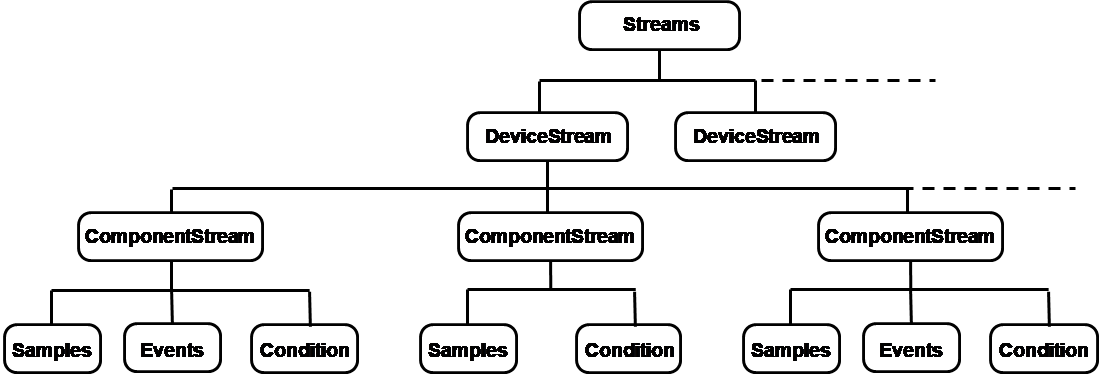
\includegraphics[width=1.0\textwidth]{figures/streams-data-structure.png}
  \caption{Streams Data Structure}
  \label{fig:streams-data-structure}
\end{figure}

\lst{example-of-devicestream} is a sample from an \gls{mtconnectstreams} XML document that contains the response from an \gls{agent} representing two pieces of equipment, \textit{mill-1} and \textit{mill-2}. The data from each piece of equipment is reported in a separate \gls{devicestream} container. 

\begin{lstlisting}[firstnumber=1,escapechar=|,%
    caption={Example of  DeviceStream},label={lst:example-of-devicestream}]
<MTConnectStreams ...>
  <Header ... />
  <Streams>
    <DeviceStream name="mill-1" uuid="1">
      <ComponentStream component="Device" name="mill-1"
          componentId="d1">
        <Events>
          <Availability dataItemId="avail1" name="avail"
              sequence="5"
              timestamp="2010-04-06T06:19:35.153141">
            AVAILABLE</Availability>
        </Events>
      </ComponentStream>
    </DeviceStream>
    <DeviceStream name="mill-2" uuid="2">
      <ComponentStream component="Device" name="mill-2"
          componentId="d2">
        <Events>
          <Availability dataItemId="avail2" name="avail" 
              sequence="15"
              timestamp="2010-04-06T06:19:35.153141">
            AVAILABLE</Availability>
        </Events>
      </ComponentStream>
    </DeviceStream>
  </Streams>
</MTConnectStreams>
\end{lstlisting}

In \lst{example-of-devicestream}, it should be noted that the \glspl{sequence number} are unique across the two pieces of equipment. Client software applications \MUSTNOT assume that the \gls{events} and \gls{samples} sequence numbers are strictly in sequence. All sequence numbers \MAYNOT be included. For instance, such a case would occur when HTTP filtering is applied to the request and the \gls{sample category}, \gls{event category}, and \gls{condition category} data types for other components are not returned. Another case would occur when an \gls{agent} is supporting more than one piece of equipment and data from only one piece of equipment is requested. Refer to MTConnect Standard \citetitle{MTCPart1}, \textit{Section 5} for more information on \glspl{sequence number}.


\subsection{Streams}

\gls{streams} is a container type XML element that \must contain only \gls{devicestream} elements.  \gls{streams} \may contain any number of \gls{devicestream} elements.  If there is no data to be reported for a request for data, an \gls{mtconnectstreams} document \must be returned with an empty \gls{streams} container.  \glspl{data entity} \maynot be directly associated with the \gls{streams} container.

The XML schema in \fig{streams-schema-diagram} represents the structure of the \gls{streams} XML element.   

\begin{figure}[ht]
  \centering
  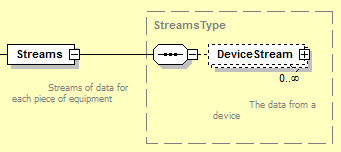
\includegraphics[width=0.75\textwidth]{figures/streams-schema-diagram.png}
  \caption{Streams Schema Diagram}
  \label{fig:streams-schema-diagram}
\end{figure}

\FloatBarrier

\tabulinesep = 5pt
\begin{longtabu} to \textwidth {
    |l|X[3l]|X[0.75l]|}
\caption{MTConnect Streams Element} \label{table:mtconnect-streams-element} \\

\hline
Element & Description & Occurrence \\
\hline
\endfirsthead

\hline
\multicolumn{3}{|c|}{Continuation of Table \ref{table:mtconnect-streams-element}}\\
\hline
Element & Description & Occurrence \\
\hline
\endhead

\gls{streams}
&
The first, or highest, level XML container element in an \gls{mtconnectstreams} \gls{response} Document provided by an \gls{agent} in response to a \gls{sample httprequest} or \gls{current httprequest} HTTP \gls{request}.
\newline There \MAY be only one \gls{streams} element in an \gls{mtconnectstreams}  \gls{response} Document for each piece of equipment represented in the document.
\newline An empty \gls{streams} container \MAY be provided to indicate that no data is available for the given \gls{request}.
\newline The \gls{streams} element \MAY contain any number of \gls{devicestream} elements, one for each piece of equipment represented in the \gls{mtconnectstreams} document.
&
1 \\ \hline

\end{longtabu}

\pagebreak

\subsection{DeviceStream}\label{sec:DeviceStream}

\gls{devicestream} is a XML container that organizes data reported from a single piece of equipment.  A \gls{devicestream} element \must be provided for each piece of equipment reporting data in an \gls{mtconnectstreams} document.

A \gls{devicestream} \may contain any number of \gls{componentstream} elements; limited to one for each component element represented in the \gls{mtconnectdevices} document.  If the response to the request for data from an \gls{agent} does not contain any data for a specific piece of equipment, an empty \gls{devicestream} element \may be created to indicate that the piece of equipment exists, but there was no data available.  In this case, there will be no \gls{componentstream} elements provided. 

\tabulinesep = 5pt
\begin{longtabu} to \textwidth {
    |l|X[3l]|X[0.75l]|}
\caption{MTConnect DeviceStream Element} \label{table:mtconnect-devicestream-element} \\

\hline
Element & Description & Occurrence \\
\hline
\endfirsthead

\hline
\multicolumn{3}{|c|}{Continuation of Table \ref{table:mtconnect-devicestream-element}}\\
\hline
Element & Description & Occurrence \\
\hline
\endhead

\gls{devicestream}
&
\glsentrydesc{devicestream}
\newline There \MAY be one or more \gls{devicestream} elements in a
\gls{streams} container; one for each piece of equipment represented in
the \gls{mtconnectstreams} document. 
&
0..* \\ \hline

\end{longtabu}

\subsubsection{XML Schema for DeviceStream}

The XML schema in \fig{devicestream-schema-diagram} represents the structure of the \gls{devicestream} XML element showing the attributes defined for \gls{devicestream} and the elements that \may be associated with \gls{devicestream}.

\begin{figure}[ht]
  \centering
  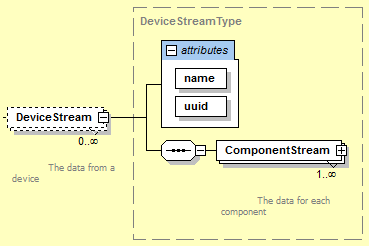
\includegraphics[width=0.7\textwidth]{figures/devicestream-schema-diagram.png}
  \caption{DeviceStream Schema Diagram}
  \label{fig:devicestream-schema-diagram}
\end{figure}
\FloatBarrier

\subsubsection{Attributes for DeviceStream}

\tbl{attributes-for-devicestream} defines the attributes that \must be provided to uniquely identify each specific piece of equipment associated with the information provided in each \gls{devicestream}.

\tabulinesep = 5pt
\begin{longtabu} to \textwidth {
    |l|X[3l]|X[0.75l]|}
\caption{Attributes for  DeviceStream} \label{table:attributes-for-devicestream} \\

\hline
Attribute & Description & Occurrence \\
\hline
\endfirsthead

\hline
\multicolumn{3}{|c|}{Continuation of Table \ref{table:attributes-for-devicestream}}\\
\hline
Attribute & Description & Occurrence \\
\hline
\endhead


\gls{name}
&
\glsentrydesc{name}
The \gls{name} associated with the piece of equipment reporting the data
contained in this \gls{devicestream} container.
\newline \gls{name} is a required attribute.
\newline The value reported for \gls{name} \MUST be the same as the value defined
for the \gls{name} attribute of the same piece of equipment in the
\gls{mtconnectdevices} document
\newline An \gls{nmtoken} XML type.
\newline \textbf{WARNING}: \gls{name} may become an optional attribute in future versions of the MTConnect Standard.
&
1 \\
\hline

\gls{uuid}
&
The \gls{uuid} associated with the piece of equipment reporting the data contained in this \gls{devicestream} container.
\newline \gls{uuid} is a required attribute. 
\newline The value reported for \gls{uuid} \MUST be the same as the value defined
for the \gls{uuid} attribute of the same piece of equipment in the
\gls{mtconnectdevices} document.
&
1 \\
\hline


\end{longtabu}

\subsubsection{Elements for DeviceStream}

\tbl{elements-for-devicestream} lists the XML element(s) that \may be provided in the \gls{devicestream} XML element.  

\tabulinesep = 5pt
\begin{longtabu} to \textwidth {
    |l|X[3l]|X[0.75l]|}
\caption{Elements for DeviceStream} \label{table:elements-for-devicestream} \\

\hline
Element & Description & Occurrence \\
\hline
\endfirsthead

\hline
\multicolumn{3}{|c|}{Continuation of Table \ref{table:elements-for-devicestream}}\\
\hline
Element & Description & Occurrence \\
\hline
\endhead

\gls{componentstream}
&
\glsentrydesc{componentstream}
\newline Any number of \gls{componentstream} elements \MAY be provided
in a \gls{devicestream} container.
\newline There \MUST be a separate \gls{componentstream} XML element
for each of the \glspl{structural element} (\gls{device} elements, \gls{top level}
\gls{component} elements, or \gls{lower level} \gls{component} elements)
defined for that piece of equipment in the associated \gls{mtconnectdevices} XML document. A \gls{componentstream}
representing a \gls{structural element} will only appear if there is data reported for that \gls{structural element}. 
&
0..* \\
\hline

\end{longtabu}

\subsection{ComponentStream}\label{sec:ComponentStream}

\gls{componentstream} is a XML container that organizes the data associated with each \gls{structural element} (\gls{device} element, \gls{top level} \gls{component}, or \gls{lower level} \gls{component} element) defined for that piece of equipment in the associated \gls{mtconnectdevices} XML document.  The data reported in each \gls{componentstream} element \must be grouped into individual XML containers based on the value of the \gls{category} attribute (\gls{sample category}, \gls{event category}, or \gls{condition category}) defined for each \gls{data entity} in the \gls{mtconnectdevices} XML document.  These containers are \gls{samples}, \gls{events}, and \gls{conditions}.   

\subsubsection{XML Schema for ComponentStream}

The XML schema in \fig{componentstream-schema-diagram} represents the structure of a \gls{componentstream} XML element showing the attributes defined for \gls{componentstream} and the elements that \may be associated with \gls{componentstream}.

\begin{figure}[ht]
  \centering
  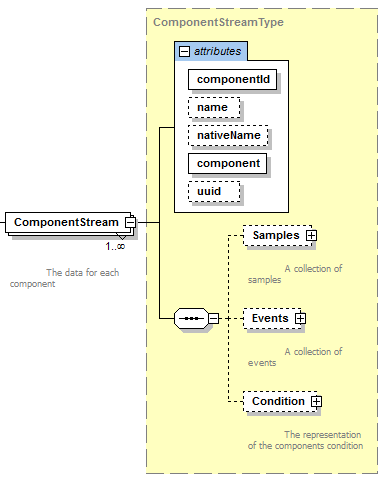
\includegraphics[width=0.7\textwidth]{figures/componentstream-schema-diagram.png}
  \caption{ComponentStream Schema Diagram}
  \label{fig:componentstream-schema-diagram}
\end{figure}

\FloatBarrier

\gls{componentstream} is similar to \gls{devicestream} in that the attributes uniquely identify the \gls{structural element} with which the data reported is directly associated.  This information does not have to be repeated for each \gls{data entity}.   In the case of the \gls{devicestream}, the attributes uniquely identify the piece of equipment associated with the data.   In the case of the \gls{componentstream}, the attributes identify the specific \gls{structural element} within a piece of equipment associated with each \gls{data entity}.  

\subsubsection{Attributes for ComponentStream}

The \tbl{attributes-for-componentstream} defines the attributes used to uniquely identify the specific \gls{structural element}(s) of a piece of equipment associated with the data reported in the \gls{mtconnectstreams} document.  


\tabulinesep = 5pt
\begin{longtabu} to \textwidth {
    |l|X[3l]|X[0.75l]|}
\caption{Attributes for ComponentStream} \label{table:attributes-for-componentstream} \\

\hline
Attribute & Description & Occurrence \\
\hline
\endfirsthead

\hline
\multicolumn{3}{|c|}{Continuation of Table \ref{table:attributes-for-componentstream}}\\
\hline
Attribute & Description & Occurrence \\
\hline
\endhead

\gls{componentid} 
&
The identifier of the \gls{structural element} (\gls{device} element, \gls{top level} \gls{component} element, or \gls{lower level} \gls{component} element) as defined by the \gls{id} attribute of the corresponding \gls{structural element} in the \gls{mtconnectdevices} XML document.
\newline \gls{componentid} is a required attribute.
\newline The identifier \MUST be the same as that defined in the \gls{mtconnectdevices} document to associate the data reported in the \gls{componentstream} container with the \gls{structural element} identified
in the \gls{mtconnectdevices} document.
&
1 \\
\hline


\gls{name}
&
The name of the \gls{componentstream} element.
\newline \gls{name} is an optional attribute.
\newline If \gls{name} is not defined for a specific \gls{structural element} in the
\gls{mtconnectdevices} document, it \MUSTNOT be provided for the corresponding \gls{componentstream} element in the \gls{mtconnectstreams} document.
\newline If \gls{name} is defined for a specific \gls{structural element} in the \gls{mtconnectdevices} document, it \MAY be provided for the corresponding \gls{componentstream} element in the \gls{mtconnectstreams} document.
\newline If provided, the value reported for name \MUST be the same as the
value defined for the name attribute of the corresponding \gls{structural element} (\gls{device} element, \gls{top level} \gls{component} element, or \gls{lower level} \gls{component} element) defined in the \gls{mtconnectdevices} XML document.
\newline An \gls{nmtoken} XML type.
&
0..1 \\
\hline

\gls{nativename}
&
\gls{nativename} identifies the common name normally associated with
the \gls{componentstream} element.
\newline \gls{nativename} is an optional attribute.
\newline If \gls{nativename} is not defined for a specific \gls{structural element} in the \gls{mtconnectdevices} document, it \MUSTNOT be provided for the
corresponding \gls{componentstream} element in the
\gls{mtconnectstreams} document.
\newline If \gls{nativename} is defined for a specific \gls{structural element} in the
\gls{mtconnectdevices} document, it \MAY be provided for the
corresponding \gls{componentstream} element in the
\gls{mtconnectstreams} document.
\newline If provided, the value reported for \gls{nativename} \MUST be the same as the value defined for the \gls{nativename} attribute of the corresponding
\gls{structural element} (\gls{device} element, \gls{top level} \gls{component} element,
or \gls{lower level} \gls{component} element) defined in the
\gls{mtconnectdevices} XML document.
&
0..1 \\
\hline

\gls{component componentstream}
&
\gls{component componentstream} identifies the \gls{structural element} (\gls{device}, \gls{top level} \gls{component}, or \gls{lower level} \gls{component}) associated with the
\gls{componentstream} element.
\newline \gls{component componentstream} is a required attribute.
\newline The value reported for component \MUST be the same as the value
defined for the Element Name of the XML container representing the
corresponding \gls{structural element} (\gls{device} element, \gls{top level}
\gls{component} element, or \gls{lower level} \gls{component} element) defined in
the \gls{mtconnectdevices} XML document.
\newline Examples of \gls{component} are \gls{device}, \gls{axes}, \gls{controller},
\gls{linear}, \gls{electric} and \gls{loader}.
&
1 \\
\hline

\gls{uuid}
&
\gls{uuid} of the \gls{componentstream} element.
\newline \gls{uuid} is an optional attribute.
\newline If \gls{uuid} is not defined for a specific \gls{structural element} in the
\gls{mtconnectdevices} document, it \MUSTNOT be provided for the
corresponding \gls{componentstream} element in the
\gls{mtconnectstreams} document.
\newline If \gls{uuid} is defined for a specific \gls{structural element} in the
\gls{mtconnectdevices} document, it \MAY be provided for the
corresponding \gls{componentstream} element in the
\gls{mtconnectstreams} document, but it is not required.
\newline If provided, the value reported for \gls{uuid} \MUST be the same as the
value defined for the \gls{uuid} attribute of the corresponding \gls{structural element} (\gls{device} element, \gls{top level} \gls{component} element, or \gls{lower level} \gls{component} element) defined in the \gls{mtconnectdevices}
XML document.
&
0..1 \\
\hline


\end{longtabu}

\subsubsection{Elements for ComponentStream}

In the \gls{componentstream} container, an \gls{agent} \must organize the data reported in each \gls{componentstream} into individual \gls{samples}, \gls{events}, or \gls{conditions} XML containers based on the value of the \gls{category} attribute (i.e., \gls{sample category}, \gls{event category}, or \gls{condition category}) defined for each \gls{data entity} defined in the \gls{mtconnectdevices} XML document.

Each \gls{componentstream} element \must include at least one \gls{events}, \gls{samples}, or \gls{conditions} XML container element.   \glspl{data entity} returned in each of the \gls{componentstream} container elements are defined in the \tbl{elements-for-componentstream}. 

\tabulinesep = 5pt
\begin{longtabu} to \textwidth {
    |l|X[3l]|X[0.75l]|}
\caption{Elements for ComponentStream} \label{table:elements-for-componentstream} \\

\hline
Element & Description & Occurrence \\
\hline
\endfirsthead

\hline
\multicolumn{3}{|c|}{Continuation of Table \ref{table:elements-for-componentstream}}\\
\hline
Element & Description & Occurrence \\
\hline
\endhead

\gls{samples}
&
An XML container type element.
\newline \gls{samples} organizes the \gls{sample category} type \glspl{data entity} defined in the \gls{mtconnectdevices} document that are reported in each
\gls{componentstream} XML element.
&
0..1 \notesign \\
\hline

\gls{events}
&
An XML container type element.
\newline \gls{events} organizes the \gls{event category} type \glspl{data entity} defined in the \gls{mtconnectdevices} document that are reported in each
\gls{componentstream} XML element.
&
0..1 \notesign \\
\hline

\gls{conditions}
&
An XML container type element.
\newline \gls{conditions} organizes the \gls{condition category} type \glspl{data entity} defined in the \gls{mtconnectdevices} document that are reported in each
\gls{componentstream} XML element.
&
0..1 \notesign \\
\hline

\end{longtabu}

\begin{note}
Note: \notesign The \gls{componentstream} element \must contain at least one of these element types.

\end{note}

\section{Data Entities}\label{sec:Data Entities}

When a piece of equipment reports values associated with \gls{dataitem} elements defined in the \gls{mtconnectdevices} document, that information is organized as \glspl{data entity} in the \gls{mtconnectstreams} document.   These \glspl{data entity} are organized in containers within each \gls{componentstream} element based on the \gls{category} attribute defined for the corresponding \gls{dataitem} in the \gls{mtconnectdevices} document:

\tab \gls{dataitem} elements defined with a \gls{category} attribute of \gls{sample category} in the \gls{mtconnectdevices} document are mapped to the \gls{samples} XML container in the associated \gls{componentstream} element.

\tab \gls{dataitem} elements defined with a \gls{category} attribute of \gls{event category} in the \gls{mtconnectdevices} document are mapped to the \gls{events} XML container in the associated \gls{componentstream} element.

\tab \gls{dataitem} elements defined with a \gls{category} attribute of \gls{condition category} in the \gls{mtconnectdevices} document are mapped to the \gls{conditions} XML container in the associated \gls{componentstream} element.

The XML tree in \fig{componentstream-xml-tree-diagram} demonstrates how \glspl{data entity} are organized in these containers.  

\begin{figure}[ht]
  \centering
  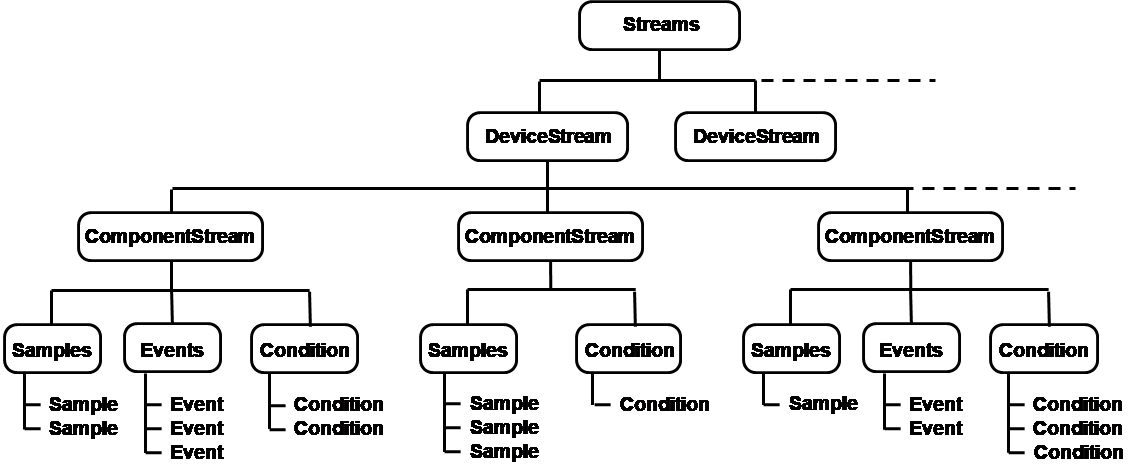
\includegraphics[width=1.0\textwidth]{figures/componentstream-xml-tree-diagram.png}
  \caption{ComponentStream XML Tree Diagram}
  \label{fig:componentstream-xml-tree-diagram}
\end{figure}
\FloatBarrier

\lst{example-of-mtconnectstreams} is an illustration of the structure of an XML document demonstrating how \glspl{data entity} are reported in a \gls{mtconnectstreams} document:

\begin{lstlisting}[firstnumber=1,escapechar=|,%
    caption={Example of  MTConnectStreams},label={lst:example-of-mtconnectstreams}]
<MTConnectStreams>
  <Header/>
  <Streams>
    <DeviceStream>
      <ComponentStream>
        <Samples>
          <Sample/>
          <Sample/>
        </Samples>
        <Events>
          <Event/>
          <Event/>
        </Events>
        <Condition>
          <Condition/>
          <Condition/>
        </Condition>
      </ComponentStream>
      <ComponentStream>
        <Samples>
          <Sample/>
          <Sample/>
        </Samples>
        <Events>
          <Event/>
          <Event/>
        </Events>
        <Condition>
          <Condition/>
          <Condition/>
        </Condition>
      </ComponentStream>
    </DeviceStream>
  </Streams>
</MTConnectStreams>
\end{lstlisting}

\begin{note}
Note: There are no specific requirements defining the sequence in which the \gls{componentstream} XML elements are organized in the \gls{mtconnectstreams} document.  They \may be organized in any sequence based on the implementation of an \gls{agent}.  The sequence in which the \gls{componentstream} XML elements appear does not impact the ability for a client software application to interpret the information that it receives in the document.
\end{note}

When an \gls{agent} responds to a  \gls{current httprequest} HTTP request, the information returned in the \gls{mtconnectstreams} document \must include the most current value for every \gls{data entity} defined in the \gls{mtconnectdevices} document subject to any filtering included within the request.

When an \gls{agent} responds to a \gls{sample httprequest} HTTP request, the information returned in the \gls{mtconnectstreams} document \must include the occurrences for each \gls{data entity} that are available to an \gls{agent} subject to filtering and the count parameter included within the request (see \citetitle{MTCPart1} for a full definition of the protocol). 

\subsection{Element Names for Data Entities}

In the \gls{mtconnectdevices} document, \glspl{data entity} are grouped as \gls{dataitem} XML elements within each \gls{device}, \gls{top level} \gls{component}, and \gls{lower level} \gls{component} \gls{structural element}.  The \glspl{data entity} reported in the \gls{mtconnectstreams} document associated with each of these \glspl{structural element} are represented with an \gls{element name} based on the \gls{category} and \gls{type} defined for each of the \gls{dataitem} elements in the \gls{mtconnectdevices} document.

\subsubsection{Element Names when MTConnectDevices category is SAMPLE or EVENT}

The \glspl{data entity} reported in the \gls{mtconnectstreams} document associated with each \gls{dataitem} element defined in the \gls{mtconnectdevices} document with a \gls{category} attribute of \gls{sample category} or \gls{event category} \must be identified in the \gls{mtconnectstreams} document with an \gls{element name} derived from the \gls{type} attribute defined for that \gls{dataitem} element in the \gls{mtconnectdevices} document.

\lst{example-of-dataitem-in-mtconnectdevices} describes the most common method used to derive the \gls{element name} for a \gls{data entity} reported in the \gls{mtconnectstreams} document from the information describing that \gls{dataitem} element in the \gls{mtconnectdevices} document:

\ulheading{DataItem Represented in the MTConnectDevices Document}

\begin{lstlisting}[firstnumber=1,escapechar=|,%
    caption={DataItem Represented in MTConnectDevices Document},label={lst:example-of-dataitem-in-mtconnectdevices}]
<DataItem type="AXIS_FEEDRATE" id="xf" name="Xfrt"
    category="SAMPLE" units="MILLIMETER/SECOND"
    nativeUnits="MILLIMETER/SECOND/>
\end{lstlisting}

\begin{itemize}
\item \gls{dataitem}:  The XML \gls{element name} for this \gls{data entity}.  

\begin{note}
Note:  \gls{element name} must not be confused with the name attribute for the data item element.
\end{note}

\item \gls{type}, \gls{category}, \gls{units}, and \gls{nativeunits}:  Attributes that provide additional information regarding each data item in the \gls{mtconnectdevices} document.  
\end{itemize}

\ulheading{Response Format reported in the MTConnectStreams Document}

\begin{lstlisting}[firstnumber=1,escapechar=|,%
    caption={Response Format reported in the MTConnectStreams Document},label={lst:example-of-dataitem-in-mtconnectstreams}]
<AxisFeedrate name="Xfrt" sequence="61315517"  
    timestamp="2016-07-28T02:06:01.364428Z" 
    dataItemId="xf">10.83333</AxisFeedrate>
\end{lstlisting}

\begin{itemize}
\item \gls{axisfeedrate sample}:  The \gls{element name} provided in the \gls{mtconnectstreams} response format for the data item. The \gls{element name} for a data item is defined by the \gls{type} attribute of \gls{axisfeedrate sample} in the \gls{mtconnectdevices} document.  The \gls{element name} \must be provided in Pascal case format (first letter of each word is capitalized).  
\end{itemize}

\subsubsection{Changes to Element Names when representation attribute is used}

The \gls{element name} for a \gls{data entity} reported in the \gls{mtconnectstreams} document is extended when the \gls{representation} attribute is used to further describe that \gls{dataitem} element in the \gls{mtconnectdevices} document.

When a \gls{dataitem} element is defined in the \gls{mtconnectdevices} document with a \gls{representation} attribute of \gls{timeseries representation}\DIFaddbegin \DIFadd{, \gls{dataset}, }\DIFaddend or \gls{discrete representation}, the XML \gls{element name} for the associated \gls{data entity} reported in the \gls{mtconnectstreams} document \must be extended by adding the value of the \gls{representation} attribute to the \gls{element name}.

For example, the \gls{dataitem} element \gls{angularvelocity sample} with a \gls{representation} attribute defined as \gls{timeseries representation} \must be transformed to the \gls{element name} \glsrepresentation{angularvelocity sample}.

Similarly, the \gls{dataitem} element \gls{partcount} with a \gls{representation} attribute defined as \gls{discrete representation} \must be transformed to the \gls{element name} \glsrepresentation{partcount}.

\subsubsection{Element Names when MTConnectDevices category is CONDITION}

\glspl{data entity} defined in the \gls{mtconnectdevices} document with a \gls{category} attribute of \gls{condition category} are reported with an \gls{element name} that is defined differently from other \gls{data entity} \glspl{type}.  The \gls{element name} for these \glspl{data entity} are defined based on the \gls{fault state} (\gls{normal}, \gls{warning}, or \gls{fault}) associated with each \gls{data entity} at the time that a value for that \gls{data entity} is reported.  See \sect{Element Names for Condition} and \sect{Unavailability of Fault State for Condition} for details on how these \glspl{data entity} are reported in the \gls{mtconnectstreams} document.

\subsection{Samples Container}

\gls{samples} is a XML container type element.   \gls{samples} organizes the \glspl{data entity} returned in the \gls{mtconnectstreams} XML document for those \gls{dataitem} elements defined with a \gls{category} attribute of \gls{sample category} in the \gls{mtconnectdevices} document.

A separate \gls{samples} container will be provided for the data returned for the \gls{dataitem} elements associated with each \gls{structural element} of a piece of equipment defined in the \gls{mtconnectdevices} document.

\tabulinesep = 5pt
\begin{longtabu} to \textwidth {
    |l|X[3l]|X[0.75l]|}
\caption{MTConnect Samples Element} \label{table:mtconnect-samples-element} \\

\hline
Element & Description & Occurrence \\
\hline
\endfirsthead

\hline
\multicolumn{3}{|c|}{Continuation of Table \ref{table:mtconnect-samples-element}}\\
\hline
Element & Description & Occurrence \\
\hline
\endhead

\gls{samples}
&
\glsentrydesc{samples} 
\newline A separate \gls{samples} container \MUST be provided for each
\gls{componentstream} element for which data is returned for a \gls{dataitem}
element defined in the \gls{mtconnectdevices} document with a \gls{category}
attribute of \gls{sample category}.
\newline If provided in the document, a \gls{samples} XML container \MUST contain at least one \gls{sample} element.
&
0..1 \\
\hline

\end{longtabu}


\subsection{Sample Data Entities}

A \gls{sample} XML element provides the information and data reported from a piece of equipment for those \gls{dataitem} elements defined with a \gls{category} attribute of \gls{sample category} in the \gls{mtconnectdevices} document.

\gls{sample} is an abstract type XML element and will never appear directly in the \gls{mtconnectstreams} XML document.  As an abstract \gls{type} XML element, \gls{sample} will be replaced in the XML document by a specific \gls{type} of \gls{sample} specified by the \gls{element name} for that \gls{data entity}.  The different \glspl{type} of \gls{sample} elements are defined in \sect{Sample Element Names}.  Examples of XML elements representing \gls{sample} include \glselementname{pathposition sample}, \glselementname{temperature sample}. 

\pagebreak

\tabulinesep = 5pt
\begin{longtabu} to \textwidth {
    |l|X[3l]|X[0.75l]|}
\caption{MTConnect Sample Element} \label{table:mtconnect-sample-element} \\

\hline
Element & Description & Occurrence \\
\hline
\endfirsthead

\hline
\multicolumn{3}{|c|}{Continuation of Table \ref{table:mtconnect-sample-element}}\\
\hline
Element & Description & Occurrence \\
\hline
\endhead

\gls{sample}
&
\glsentrydesc{sample} 
\newline \gls{sample} is an abstract type XML element. It is replaced in the \gls{mtconnectstreams} document by a specific type of \gls{sample} element.
\newline There \MAY be multiple types of \gls{sample} elements in a \gls{samples} container.
&
1..* \\
\hline
\end{longtabu}

\subsubsection{XML Schema Structure for Sample}

The XML schema in \fig{sample-schema-diagram} represents the structure of a \gls{sample} XML element showing the attributes defined for \gls{sample} elements.

\begin{figure}[ht]
  \centering
  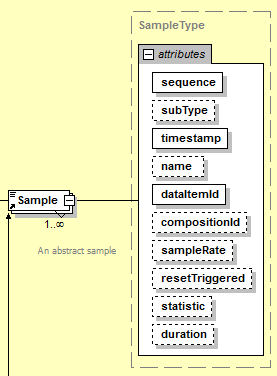
\includegraphics[width=0.5\textwidth]{figures/sample-schema-diagram.png}
  \caption{Sample Schema Diagram}
  \label{fig:sample-schema-diagram}
\end{figure}

\pagebreak

\subsubsection{Attributes for Sample}

The \tbl{attributes-for-sample} defines the attributes used to provide additional information for a \gls{sample} XML element.   


\tabulinesep = 5pt
\begin{longtabu} to \textwidth {
    |l|X[3l]|X[0.75l]|}
\caption{Attributes for  Sample} \label{table:attributes-for-sample} \\

\hline
Attribute & Description & Occurrence \\
\hline
\endfirsthead

\hline
\multicolumn{3}{|c|}{Continuation of Table \ref{table:attributes-for-sample}}\\
\hline
Attribute & Description & Occurrence \\
\hline
\endhead

\gls{sequence} 
&
A number representing the sequential position of an occurrence of the
\gls{sample} in the data buffer of an \gls{agent}.
\newline \gls{sequence} is a required attribute.
\newline \gls{sequence} \MUST have a value represented as an unsigned 64-bit
value from 1 to $2^{64}-1$.
&
1 \\
\hline

\gls{subtype} 
&
The \gls{subtype} of the \gls{data entity}.
\newline \gls{subtype} is an optional attribute.
\newline \gls{subtype} \MUST match the \gls{subtype} attribute of the \gls{dataitem} element as defined in the \gls{mtconnectdevices} document that the
\gls{sample} element represents. 
&
0..1 \\
\hline

\gls{timestamp} 
&
The most accurate time available to a piece of equipment that represents
the point in time that the data reported for the \gls{sample} was measured.
\newline When the \gls{sample} element represents a \gls{dataitem} element defined in the \gls{mtconnectdevices} document with a \gls{representation} or
\gls{statistic} attribute, \gls{timestamp} \MUST represent the time that the
data collection was completed.
\newline \gls{timestamp} is a required attribute.
&
1 \\
\hline

\gls{name} 
&
The name of the \gls{sample} element.
\newline \gls{name}  is an optional attribute.
\newline \gls{name}  \MUST match the \gls{name}  attribute of the \gls{dataitem} element defined in the \gls{mtconnectdevices} document that the \gls{sample}
element represents.
\newline An \gls{nmtoken} XML type. 
&
0..1 \\
\hline

\gls{dataitemid} 
&
The unique identifier for the \gls{sample} element.
\newline \gls{dataitemid} is a required attribute.
\newline \gls{dataitemid} \MUST match the id attribute of the \gls{dataitem}
element defined in the \gls{mtconnectdevices} document that the
\gls{sample} element represents. 
&
1 \\
\hline

\gls{samplerate} 
&
The rate at which successive samples of the value of a data item are
recorded. \gls{samplerate} is expressed in terms of samples per second.
\newline \gls{samplerate} is an optional attribute.
\newline If the \gls{samplerate} is smaller than one, the number can be represented as a decimal type floating-point number. For example, a rate of 1 per 10 seconds would be 0.1
\newline \gls{samplerate} \MUST be provided when the representation
attribute of the \gls{dataitem} element defined in the
\gls{mtconnectdevices} document that this \gls{sample} element represents is \gls{timeseries representation}.
\newline For \gls{dataitem} elements where the representation attribute
defined in the \gls{mtconnectdevices} document that this \gls{sample}
element represents is not \gls{timeseries representation}, it MUST be assumed that the data reported is represented by a single value and \gls{samplerate} \MUSTNOT be reported in the \gls{mtconnectstreams} document.
&
0..1 \\
\hline

\gls{statistic}
&
The type of statistical calculation defined by the \gls{statistic} attribute
of the \gls{dataitem} element defined in the \gls{mtconnectdevices}
document that this \gls{sample} element represents.
\newline \gls{statistic} is an optional attribute.
&
0..1 \\
\hline

\gls{duration}
&
The time-period over which the data was collected.
\newline \gls{duration} is an optional attribute.
\newline \gls{duration} \MUST be provided when the\gls{statistic} attribute of the \gls{dataitem} element is defined in the \gls{mtconnectdevices} document
that this \gls{sample} element represents.
&
0..1 \\
\hline

\gls{resettriggered}
&
For those \gls{dataitem} elements that report data that may be periodically reset to an initial value, \gls{resettriggered} identifies when a reported value has been reset and what has caused that reset to occur.
\newline \gls{resettriggered} is an optional attribute.
\newline \gls{resettriggered} \MUST only be provided for the specific
occurrence of a \gls{data entity} reported in the \gls{mtconnectstreams} document when the reset occurred and \MUSTNOT be provided for any other occurrence of the \gls{data entity} reported in a \gls{mtconnectstreams} document.
&
0..1 \\
\hline

\gls{compositionid}
&
The identifier of the \gls{composition} element defined in the \gls{mtconnectdevices} document associated with the data reported for the \gls{sample} element.
\newline \gls{compositionid} is an optional attribute.
&
0..1 \\
\hline
\end{longtabu}

\paragraph{duration Attribute for Sample}\mbox{}

\gls{sample} elements that represent the result of a computed value of a statistic \must contain a \gls{duration} attribute.  For these \glspl{data entity}, the \gls{timestamp} associated with the \gls{sample} \must reference the time the data collection was completed.  \gls{timestamp} \MUSTNOT represent any other time associated with the data collection or the calculation of the statistic.  The actual time the interval began can be computed by subtracting the \gls{duration} from the \gls{timestamp}.

Two \gls{sample} elements \may have overlapping time periods when statistics are computed at different frequencies.  For example, there may be two \glspl{data entity} reporting a statistic representing the average value for the readings of the same measured signal calculated over one and five minute intervals.  These \glspl{data entity} can both have the same start time for their calculations (e.g., 05:10:00), but the \gls{timestamp} and \gls{duration} will be 05:11:00 and 60 seconds, respectively, for the \gls{data entity} reporting the one-minute average and 05:15:00 and 300 seconds, respectively, for the \gls{data entity} reporting the five-minute average.  This allows for varying statistical methods to be applied with different interval lengths each having different values for the \gls{timestamp} and \gls{duration} attributes.  

\paragraph{resetTriggered Attribute for Sample}\mbox{}

Some \glspl{data entity} \may have their reported value reset to an initial value.  These reset actions may be based upon a specific elapsed time or may be triggered by a physical or logical reset action that causes the reset to occur.   Examples of \glspl{data entity} that \may have their reported value reset to an initial value are \glspl{data entity} representing a counter, a timer, or a statistic.

\gls{resettriggered} defines the \gls{type} of reset action that caused the value of the reported data to be reset.  The value reported for \gls{resettriggered} \may be defined by the \gls{resettrigger} element for the \gls{data entity} in the \gls{mtconnectdevices} document that this \gls{sample} element represents.  If the \gls{resettrigger} element is not defined in the \gls{mtconnectdevices} document, a \gls{resettriggered} attribute \should be reported in the \gls{mtconnectstreams} document if the \gls{type} of reset action can be determined and reported by the piece of equipment.

\gls{resettriggered} \must only be reported for the first occurrence of a \gls{data entity} after a reset action has occurred and \mustnot be provided for any other occurrence of the \gls{data entity} reported in a \gls{mtconnectstreams} document.  When a reset occurs, the piece of equipment \must report an occurrence of the \gls{data entity} that was reset even if that occurrence of the \gls{data entity} would normally be suppressed based on the filtering criteria established in the \gls{mtconnectdevices} document that this \gls{sample} element represents.

The \tbl{values-for-resettriggered} provides the values that \may be reported for \gls{resettriggered}:    

\tabulinesep = 5pt
\begin{longtabu} to \textwidth {
    |l|X[3l]|}
\caption{Values for resetTriggered} \label{table:values-for-resettriggered} \\

\hline
Value for resetTriggered & Description\\
\hline
\endfirsthead

\hline
\multicolumn{2}{|c|}{Continuation of Table \ref{table:values-for-resettriggered}} \\
\hline
Value for resetTriggered & Description\\
\hline
\endhead

\gls{actioncomplete} & 
The value of the \gls{data entity} that is measuring an action or
operation was reset upon completion of that action or
operation. \\ \hline 

\gls{annual} & 
The value of the \gls{data entity} was reset at the end of a 12-month period.\\ \hline 

\gls{day} & 
The value of the \gls{data entity} was reset at the end of a 24-hour
period.\\ \hline 

\gls{maintenance}
& 
The value of the \gls{data entity} was reset upon completion of a maintenance event.
\\ \hline 

\gls{manual value} &
The value of the \gls{data entity} was reset based on a physical reset action. \\ \hline

\gls{month} & 
The value of the \gls{data entity} was reset at the end of a monthly
period. \\ \hline 

\gls{poweron} & 
The value of the \gls{data entity} was reset when power was
applied to the piece of equipment after a planned or unplanned
interruption of power has occurred.\\ \hline 

\gls{shift} & 
The value of the \gls{data entity} was reset at the end of a work
shift.\\ \hline 

\gls{week} & 
The value of the \gls{data entity} was reset at the end of a 7-day
period.\\ \hline 




\end{longtabu}


\subsubsection{Response for SAMPLE category DataItem Elements with a representation Attribute of TIME\_SERIES}
\label{sec:Response for SAMPLE category DataItem Elements with a representation Attribute of TIME_SERIES}

\gls{sample category} category \gls{dataitem} elements defined in the \gls{mtconnectdevices} document with a \gls{representation} attribute of \gls{timeseries representation} \must be represented in the \gls{mtconnectstreams} document as \gls{sample} elements that report data that includes multiple values representing a series of readings of a measured value taken at a specific sample rate.   Such a \gls{dataitem} element can be defined for collecting high frequency readings of a measured value and then providing the entire series of values to a client software application as the data reported for a single \gls{data entity}.  In this case, the \gls{samplecount} and \gls{samplerate} attributes \must be provided. 

\begin{note}
Note: \gls{samplecount} is an attribute that \must only be provided for \gls{sample} elements that represent \gls{sample category} category \gls{dataitem} elements defined in the \gls{mtconnectdevices} document with a \gls{representation} attribute of \gls{timeseries representation}.  

\end{note}

The \gls{cdata} provided for the \gls{data entity} \must be a series of space delimited floating-point numbers.  The number of values \must match the \gls{samplecount}.  

\paragraph{XML Schema Structure for Sample when reporting Time Series Data}\mbox{}

The XML schema in \fig{abstimeseries-schema-diagram}  represents the extended structure of a \gls{sample} XML element that represents a \gls{sample category} category \gls{dataitem} element defined in the \gls{mtconnectdevices} document with a \gls{representation} attribute of \gls{timeseries representation}. 

\begin{figure}[ht]
  \centering
  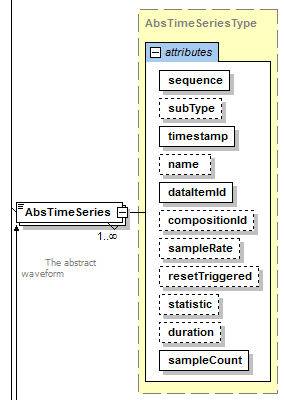
\includegraphics[width=0.5\textwidth]{figures/abstimeseries-schema-diagram.png}
  \caption{AbsTimeSeries Schema Diagram}
  \label{fig:abstimeseries-schema-diagram}
\end{figure}
\FloatBarrier

\begin{note}
Note: The \gls{abstimeseries} element shown in the XML schema is an abstract type element and will be replaced in the \gls{mtconnectstreams} document by the \gls{element name} derived from the \gls{type} attribute defined for the associated \gls{dataitem} element defined in the \gls{mtconnectdevices} document.

\end{note}

\paragraph{Attributes for a Sample when reporting Time Series Data}\mbox{}

\tbl{mtconnect-samplecount-attribute} defines the additional attribute provided for a \gls{sample} XML element that represents a \gls{sample category} category \gls{dataitem} element defined in the \gls{mtconnectdevices} document with a representation attribute of \gls{timeseries representation}. 

\tabulinesep = 5pt
\begin{longtabu} to \textwidth {
    |l|X[3l]|X[0.75l]|}
\caption{MTConnect sampleCount Attribute} \label{table:mtconnect-samplecount-attribute} \\

\hline
Attribute & Description & Occurrence \\
\hline
\endfirsthead

\hline
\multicolumn{3}{|c|}{Continuation of Table \ref{table:mtconnect-samplecount-attribute}}\\
\hline
Attribute & Description & Occurrence \\
\hline
\endhead

\gls{samplecount}
&
The number of readings reported in the data returned for the \gls{dataitem}
element defined in the \gls{mtconnectdevices} document that this
\gls{sample} element represents.
\newline \gls{samplecount} is an optional attribute.
\newline \gls{samplecount} \MUST be provided when the representation
attribute of the \gls{dataitem} element is \gls{timeseries representation}.
\newline \gls{samplecount} \MUSTNOT be provided when the
\gls{representation} attribute is defined as \gls{discrete representation} or \gls{value representation}, or
when it is not defined.
&
0..1 \\
\hline

\end{longtabu}


\DIFaddbegin \subsubsection{\DIFadd{Response for SAMPLE category DataItem Elements with a representation attribute of DATA_SET}}
\label{sec:Response for SAMPLE category DataItem Elements with a representation attribute of DATA_SET}

\DIFadd{\gls{sample category} category \gls{dataitem} elements defined in the \gls{mtconnectdevices} document with a \gls{representation} attribute of \gls{dataset} \MUST be represented in the \gls{mtconnectstreams} document as \gls{sample} XML Elements reported as a  \gls{data set} of \glspl{key-value pair}. \gls{dataset} provides the capability to report a set of related data values as a single \gls{data entity}.
}

\DIFadd{The \gls{sample} XML Element acts as a container for \gls{entry} elements to provide a \gls{data set} of \glspl{key-value pair} where each \gls{key model} attribute of the \gls{entry} \MUST be unique and acts as the identity of the \gls{key-value pair}. The CDATA of the \gls{entry} element represents the value portion of the \gls{key-value pair} and has the same constraints as the \gls{data entity} type defined for the \gls{dataitem} \gls{type}.
}

\paragraph{\DIFadd{XML Schema Structure for Sample when reporting Data Set data}}\DIFadd{\mbox{}
}\label{sec:XML Schema Structure for SAMPLE when reporting Data Set data}

\DIFadd{\fig{sample-data-set-schema-diagram} represents the XML schema of a \gls{sample} XML element that represents a \gls{sample category} category \gls{dataitem} element defined in the \gls{mtconnectdevices} document with a \gls{representation} attribute of \gls{dataset}.
}\begin{figure}[ht]
  \centering
  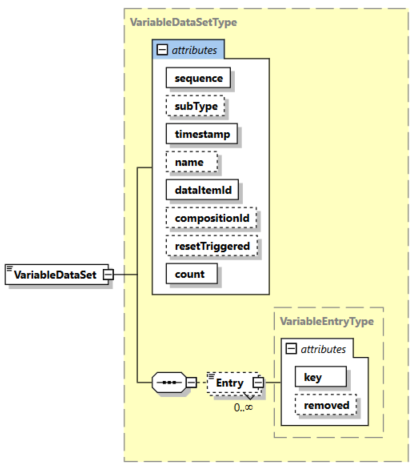
\includegraphics[width=1.0\textwidth]{figures/sample-data-set-schema-diagram.png}
  \caption{\DIFaddFL{Sample Data Set Schema Diagram}}
  \label{fig:sample-data-set-schema-diagram}
\end{figure}
\FloatBarrier

\paragraph{\DIFadd{Attributes for Sample when reporting Data Set data}}\DIFadd{\mbox{}
}\label{sec:Attributes for SAMPLE when reporting Data Set data}

\DIFadd{\tbl{attributes-for-dataset} defines the additional attribute provided for a \gls{sample} XML element that represents a \gls{sample category} category \gls{dataitem} element defined in the \gls{mtconnectdevices} document with a \gls{representation} attribute of \gls{dataset}.
}


\begin{longtabu} to \textwidth{|l|X[3l]|l|}
\caption{\DIFadd{Attributes for DataSet}} \label{table:attributes-for-dataset} \\

\hline
\DIFadd{Attribute }& \DIFadd{Description }& \DIFadd{Occurrence }\\
\hline
\endfirsthead

\hline
\multicolumn{3}{|c|}{Continuation of Table \ref{table:attributes-for-dataset}}\\
\hline
\DIFadd{Attribute }& \DIFadd{Description }& \DIFadd{Occurrence }\\
\hline
\endhead





\DIFadd{\gls{count}
}&
\DIFadd{Represents the number of \glspl{key-value pair} represented as \gls{entry} elements as the contents of the \gls{sample} element.
}\newline \DIFadd{\gls{count model} \MUST be provided when the \gls{representation} attribute of the \gls{dataitem} element is \gls{dataset}.
}\newline \DIFadd{\gls{count model} \MUSTNOT be provided when the \gls{representation} attribute is defined as \gls{discrete representation}, \gls{timeseries representation}, or \gls{value representation}, or when it is not defined.
}&
\DIFadd{0..1 }\\
\hline\end{longtabu}

\paragraph{\DIFadd{Elements for Sample when reporting Data Set data}}\DIFadd{\mbox{}
}\label{sec:Elements for SAMPLE when reporting Data Set data}

\DIFadd{\tbl{elements-for-dataset} defines the elements provided for a \gls{sample} XML element that represents a \gls{sample category} category \gls{dataitem} element defined in the \gls{mtconnectdevices} document with a \gls{representation} attribute of \gls{dataset}. \gls{entry} is the only child element that \MAY be associated with a \gls{data entity} with a \gls{representation} attribute of \gls{dataset}. Each \gls{entry} element represents a unique \gls{key-value pair}. 
}


\begin{longtabu} to \textwidth{|l|X[3l]|l|}
\caption{\DIFadd{Elements for DataSet}} \label{table:elements-for-dataset} \\

\hline
\DIFadd{Element }& \DIFadd{Description }& \DIFadd{Occurrence }\\
\hline
\endfirsthead

\hline
\multicolumn{3}{|c|}{Continuation of Table \ref{table:elements-for-dataset}}\\
\hline
\DIFadd{Element }& \DIFadd{Description }& \DIFadd{Occurrence }\\
\hline
\endhead





\DIFadd{\gls{entry}
}&
\DIFadd{A XML element representing a \gls{key-value pair} published as part of a \gls{data set}.
}&
\DIFadd{0..* }\\
\hline\end{longtabu}

\subparagraph{\DIFadd{XML Schema Structure for Entry Element for a Data Entity}}\DIFadd{\mbox{}
}\label{sec:XML Schema Structure for Entry Element for a Data Entity}

\DIFadd{\fig{entry-element-schema-diagram} represents the XML Schema structure for a \gls{entry} XML element that represents the information published for a \gls{key-value pair}. Any number of \gls{entry} elements \MAY be provided for a \gls{data entity} defined with a \gls{representation} attribute of \gls{dataset}. 
}\begin{figure}[ht]
  \centering
  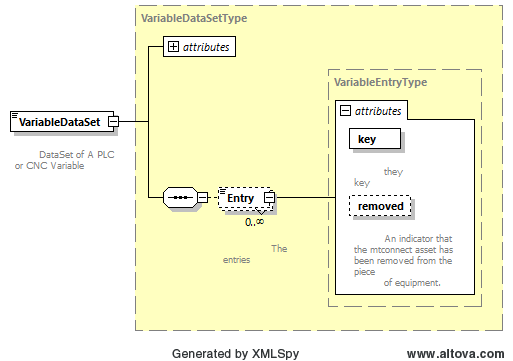
\includegraphics[width=1.0\textwidth]{figures/entry-element-schema-diagram.png}
  \caption{\DIFaddFL{Entry Element Schema Diagram}}
  \label{fig:entry-element-schema-diagram}
\end{figure}
\FloatBarrier

\DIFadd{Note: The \cfont{VariableDataSet} element shown in the XML schema is an example that illustrates the schema for a \gls{data entity} element and its associated \gls{entry} elements representing a \gls{data set}.
}

\DIFadd{The following example demonstrates how multiple \glspl{key-value pair}, each defined by an \gls{entry} element, are structured in a \gls{mtconnectstreams} document.
}\begin{lstlisting}[firstnumber=1,escapechar=|,%
    caption={Example of multiple key-value pairs Reported for a Data Entity},label={lst:example-of-multiple-key-value-pairs-reported-for-a-data-entity}]
  <VariableDataSet timestamp="..." sequence="..." count="2">
    <Entry key="a101">100.21</Entry>
    <Entry key="a102">609</Entry>
    <Entry key="a103" removed="true" />
  </VariableDataSet>
\end{lstlisting}

\subparagraph{\DIFadd{Attributes for Entry Element for a Data Entity}}\DIFadd{\mbox{}
}\label{sec:Attributes for Entry Element for a Data Entity}

\DIFadd{The \tbl{attributes-for-entry} defines the attributes provided for a \gls{entry} XML element. 
}


\begin{longtabu} to \textwidth{|l|X[3l]|l|}
\caption{\DIFadd{Attributes for Entry}} \label{table:attributes-for-entry} \\

\hline
\DIFadd{Attribute }& \DIFadd{Description }& \DIFadd{Occurrence }\\
\hline
\endfirsthead

\hline
\multicolumn{3}{|c|}{Continuation of Table \ref{table:attributes-for-entry}}\\
\hline
\DIFadd{Attribute }& \DIFadd{Description }& \DIFadd{Occurrence }\\
\hline
\endhead





\DIFadd{\gls{key model}
}&
\DIFadd{A unique identifier for each \gls{key-value pair}.
}\newline \DIFadd{The value provided for \gls{key model} \MUST be unique in any given set of \gls{entry} elements.
}\newline \DIFadd{The value provided for \gls{key model} \MUST be a XML NMTOKEN type.
}&
\DIFadd{1 }\\
\hline

\DIFadd{\gls{removed}
}&
\DIFadd{A indicator defining whether a specific \gls{key-value pair} has been removed from the set of \glspl{key-value pair} associated with this \gls{data set}.
}\newline \DIFadd{\gls{removed} is an XML Boolean type that \MUST have a value of \gls{true removed} or \gls{false removed}.
}\newline \DIFadd{\gls{true removed} indicates that the \gls{key-value pair} has been removed from the \gls{data set}.
}\newline \DIFadd{\gls{false removed} indicates that the \gls{key-value pair} has not been removed from the \gls{data set}.
}\newline \DIFadd{If not specified, the default value for \gls{removed} is \gls{false removed}
}&
\DIFadd{0..1 }\\
\hline\end{longtabu}


\DIFaddend \subsubsection{Valid Data Values for Sample}

All \gls{sample} elements reported in an \gls{mtconnectstreams} XML document \must provide a value in the \gls{cdata} of the \gls{data entity}.

The value returned in the \gls{cdata} \must be reported as either a \gls{valid data value} representing the information reported from a piece of equipment or \gls{unavailable value} when a \gls{valid data value} cannot be determined.

The \gls{valid data value} reported for a \gls{sample} represents the reading of the value of a continuously variable or analog data source.

The \gls{representation} attribute for a \gls{sample category} category \gls{dataitem} element defined in the \gls{mtconnectdevices} document specifies how an \gls{agent} \must record instances of the data associated with that data item and how often that data \must be reported as a \gls{sample} element in the \gls{mtconnectstreams} document.

The data reported for a \gls{sample} element associated with a \gls{sample category} category \gls{dataitem} element with a \gls{representation} of \gls{value representation} can be measured at any point-in-time and \must always produce a result with a single data value.  

\begin{note}
Note: If a \gls{representation} attribute is not specified in the \gls{mtconnectdevices} document for a \gls{dataitem} element, it \must be assumed that the data reported in the \gls{mtconnectstreams} document for the \gls{data entity} has a \gls{representation} type of \gls{value representation}.

\end{note}

In the case of a \gls{sample} element associated with a \gls{sample category} category \gls{dataitem} element with a \gls{representation} attribute of \gls{timeseries representation}, the data provided \must be a series of data values representing multiple sequential samples of the measured value that will be provided only at the end of the completion of a sampling period.   (See Section \sect{Response for SAMPLE category DataItem Elements with a representation Attribute of TIME_SERIES} for more information on \gls{timeseries representation} type data).

\DIFaddbegin \DIFadd{In the case of a \gls{sample} element associated with a \gls{sample category} category \gls{dataitem} element with a \gls{representation} attribute of \gls{dataset}, the data reported for each \gls{key-value pair} \MUST be provided in the same \glspl{valid data value} and units as specified by the \gls{type} attribute for the \gls{dataitem} element.
}

\DIFadd{When an \gls{agent} responds to a \gls{current request}, the information returned in the \gls{mtconnectstreams} document for a \gls{data entity} defined to represent a \gls{data set} \MUST include the full set of \glspl{key-value pair} that are valid for that \gls{data entity}. If the \gls{current request} includes an \gls{at query} }\textit{\DIFadd{query parameter}}\DIFadd{, the \gls{agent} \MUST provide the set of \glspl{key-value pair} that are valid at the specified \gls{sequence number}.
}

\DIFadd{When an \gls{agent} responds to a \gls{sample request}, the information returned in the \gls{mtconnectstreams} document for a \gls{data entity} defined to represent a \gls{data set} \MUST include only those \glspl{key-value pair} that are valid for the \gls{data entity} at each \gls{sequence number}. 
}

\DIFaddend Data values provided for a \gls{sample} \must always be a floating-point number.   In the MTConnect Standard, floating-point numbers are defined as XML xs:float \gls{type} numbers as defined by W3C.  Any of the following number formats are valid XML floating \gls{type} numbers: 1267.43233E12, -1E4, 12.78e-2, 12, 137.2847, 0, and INF.  

\begin{note}
Note: For some \gls{sample} elements, the \gls{valid data value} \may be restricted to specific formats.  See Section 6.1 of this document for a description of any restrictions of the acceptable format for \gls{valid data value}.

\end{note}

For \gls{sample} elements, a client software application can determine the appropriate accuracy of the value reported for the \gls{data entity} by applying the significantDigits attribute defined for the corresponding \gls{dataitem} element defined in the \gls{mtconnectdevices} document.

The \gls{valid data value} reported as \gls{cdata} for a \gls{sample} element \must be formatted as part of the content between the element tags in the XML element representing that \gls{data entity}.  As an example, a \glselementname{position sample} is formatted as shown in \lst{example-of-sample-position}.

\begin{lstlisting}[firstnumber=1,escapechar=|,%
    caption={Example showing CDATA of a DataItem Element},label={lst:example-of-sample-position}]
<Position sequence="112" name="Xabs"
    timestamp="2016-07-28T02:06:01.364428Z" 
    dataItemId="10">123.3333</Position>
\end{lstlisting}

In this example, the 123.3333 is the \gls{cdata} for \glselementname{position sample}.   All \gls{cdata} in a \gls{sample} element is typed, which means that the value reported for the \gls{data entity} \must be formatted as defined in Section 6.1 for each \gls{data entity} so that it can be validated.

\subsubsection{Unavailability of Valid Data Values for Sample}

If an \gls{agent} cannot determine a \gls{valid data value} for a \gls{sample} element, the value returned for the \gls{cdata} for the \gls{data entity} \must be reported as \gls{unavailable value}.

\lst{example-of-cdata-unavailable} demonstrates how an \gls{agent} reports the value for a \gls{sample} in the \gls{cdata} when it is unable to determine a \gls{valid data value}:  


\begin{lstlisting}[firstnumber=1,escapechar=|,%
    caption={Example of CDATA when Data Entity is  UNAVAILABLE},label={lst:example-of-cdata-unavailable}]
<Samples>
  <PathPosition dataItemId="p2"
      timestamp="2009-03-04T19:45:50.458305"
      subType="ACTUAL" name="Zact"
      sequence="15065113">UNAVAILABLE</PathPosition>
  <Temperature dataItemId="t6"
      timestamp="2009-03-04T19:45:50.458305" name="temp" 
      sequence="150651134">UNAVAILABLE</Temperature>
</Samples>
\end{lstlisting}

\subsection{Events Container}

\gls{events} is a XML container type element.  \gls{events} organizes the \glspl{data entity} returned in the \gls{mtconnectstreams} XML document for those \gls{dataitem} elements defined with a \gls{category} attribute of \gls{event category} in the \gls{mtconnectdevices} document.

A separate \gls{events} container will be provided for the data returned for the \gls{dataitem} elements associated with each \gls{structural element} of a piece of equipment defined in the \gls{mtconnectdevices} document.


\tabulinesep = 5pt
\begin{longtabu} to \textwidth {
    |l|X[3l]|X[0.75l]|}
\caption{MTConnect Event Element} \label{table:mtconnect-events-element} \\

\hline
Element & Description & Occurrence \\
\hline
\endfirsthead

\hline
\multicolumn{3}{|c|}{Continuation of Table \ref{table:mtconnect-events-element}}\\
\hline
Element & Description & Occurrence \\
\hline
\endhead

\gls{events}
&
\glsentrydesc{events} 
\newline A separate \gls{events} container \MUST be provided for each
\gls{componentstream} element for which data is returned for a \gls{dataitem}
element defined in the \gls{mtconnectdevices} document with a category
attribute of \gls{event category}.
\newline If provided in the document, an \gls{events} XML container \MUST contain at least one \gls{event} element.
&
0..1 \\
\hline

\end{longtabu}


\subsection{Event Data Entities}

An \gls{event} XML element provides the information and data provided from a piece of equipment for those \gls{dataitem} elements defined with a \gls{category} attribute of \gls{event category} in the \gls{mtconnectdevices} document.

\gls{event} is an abstract \gls{type} XML element and will never appear directly in the \gls{mtconnectstreams} XML document.  As an abstract \gls{type} XML element, \gls{event} will be replaced in the XML document by a specific \gls{type} of \gls{event} specified by the \gls{element name} for that \gls{data entity}.  The different \glspl{type} of \gls{event} elements are defined in \sect{Event Element Names}.  Examples of XML elements representing \gls{event} include \glselementname{block event} and \glselementname{execution event}.

\gls{event} is similar to \gls{sample}, but its value can change with unpredictable frequency.  \gls{events} do not report intermediate values.  As an example, when \glselementname{availability event} transitions from \gls{unavailable value} to \gls{available value}, there is no intermediate state that can be inferred.

\gls{event} elements \may report data values defined by a controlled vocabulary as specified in \sect{Event Element Names}, by numeric values, or by a character string representing text or a message provided by the piece of equipment. 


\tabulinesep = 5pt
\begin{longtabu} to \textwidth {
    |l|X[3l]|X[0.75l]|}
\caption{MTConnect Event Element} \label{table:mtconnect-event-element} \\

\hline
Element & Description & Occurrence \\
\hline
\endfirsthead

\hline
\multicolumn{3}{|c|}{Continuation of Table \ref{table:mtconnect-event-element}}\\
\hline
Element & Description & Occurrence \\
\hline
\endhead

\gls{event}
&
\glsentrydesc{event} 
\newline \gls{event} is an abstract type XML element. It is replaced in the
\gls{mtconnectstreams} document by a specific type of \gls{event} element.
\newline There \MAY be multiple types of \gls{event} elements in a \glspl{event} container.
&
1..* \\
\hline

\end{longtabu}


\subsubsection{XML Schema Structure for Event}

The XML schema in \fig{event-schema-diagram} represents the structure of an \gls{event} XML element showing the attributes defined for \gls{event} elements.

\begin{figure}[ht]
  \centering
  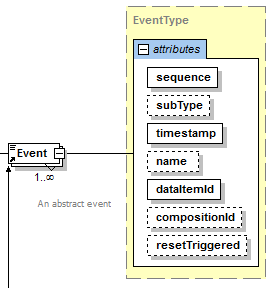
\includegraphics[width=0.5\textwidth]{figures/event-schema-diagram.png}
  \caption{Event Schema Diagram}
  \label{fig:event-schema-diagram}
\end{figure}

\FloatBarrier

\subsubsection{Attributes for Event}

\tbl{attributes-for-event} defines the attributes that \may be used to provide additional information for an \gls{event} XML element.


\tabulinesep = 5pt
\begin{longtabu} to \textwidth {
    |l|X[3l]|X[0.75l]|}
\caption{Attributes for Event} \label{table:attributes-for-event} \\

\hline
Attribute & Description & Occurrence \\
\hline
\endfirsthead

\hline
\multicolumn{3}{|c|}{Continuation of Table \ref{table:attributes-for-event}}\\
\hline
Attribute & Description & Occurrence \\
\hline
\endhead

\gls{sequence} 
&
A number representing the sequential position of an occurrence of the
\gls{event} in the data buffer of an \gls{agent}.
\newline \gls{sequence} is a required attribute.
\newline \gls{sequence} \MUST have a value represented as an unsigned 64-bit
value from 1 to $2^{64}-1$.
&
1 \\
\hline

\gls{subtype} 
&
The \gls{subtype} of the \gls{data entity}.
\newline \gls{subtype} is an optional attribute.
\newline \gls{subtype} \MUST match the \gls{subtype} attribute of the \gls{dataitem} element as defined in the \gls{mtconnectdevices} document that the
\gls{event} element represents. 
&
0..1 \\
\hline

\gls{timestamp} 
&
The most accurate time available to a piece of equipment that represents
the point in time that the data reported for the \gls{event} was measured.
\newline \gls{timestamp} is a required attribute.
&
1 \\
\hline

\gls{name} 
&
The name of the \gls{event} element.
\newline \gls{name}  is an optional attribute.
\newline \gls{name}  \MUST match the \gls{name}  attribute of the \gls{dataitem} element defined in the \gls{mtconnectdevices} document that the \gls{event}
element represents.
\newline An \gls{nmtoken} XML type. 
&
0..1 \\
\hline

\gls{dataitemid} 
&
The unique identifier for the\gls{event} element.
\newline \gls{dataitemid} is a required attribute.
\newline \gls{dataitemid} \MUST match the id attribute of the \gls{dataitem}
element defined in the \gls{mtconnectdevices} document that the
\gls{event} element represents. 
&
1 \\
\hline

\gls{resettriggered}
&
For those \gls{dataitem} elements that report data that may be periodically
reset to an initial value, \gls{resettriggered} identifies when a reported
value has been reset and what has caused that reset to occur.
\newline \gls{resettriggered} is an optional attribute.
\newline \gls{resettriggered} \MUST only be provided for the specific
occurrence of a \gls{data entity} reported in the \gls{mtconnectstreams}
document when the reset occurred and \MUSTNOT be provided for any
other occurrence of the \gls{data entity} reported in a
\gls{mtconnectstreams} document.
&
0..1 \\
\hline

\gls{compositionid}
&
The identifier of the \gls{composition} element defined in the
\gls{mtconnectdevices} document associated with the data reported for
the \gls{event} element.
\newline \gls{compositionid} is an optional attribute.
&
0..1 \\
\hline

\end{longtabu}

\subsubsection{Response for EVENT category Data Items with a representation Attribute of DISCRETE}
\label{sec:Response for EVENT category Data Items with a representation Attribute of DISCRETE}

\gls{event category} category \gls{dataitem} elements defined in an \gls{mtconnectdevices} document with a \gls{representation} attribute of \gls{discrete representation} indicate that the value of successive occurrences of the data reported in the associated \gls{event} \gls{type} \gls{data entity} in an \gls{mtconnectstreams} document \may be identical.  Duplicate values \mustnot be suppressed by an \gls{agent} since each occurrence of the data item represents a different and unique \gls{event}.

An example of an \gls{event category} category \gls{dataitem} element with a \gls{representation} attribute of \gls{discrete representation} would be a parts counter that reports the completion of each part produced, versus reporting the accumulation of parts produced over time.  In this case, the associated \gls{event} element would be represented by a \gls{data entity} with an \gls{element name} of PartCountDiscrete.  Each occurrence of this \gls{data entity} in an \gls{mtconnectstreams} document would indicate the completion of a fixed number of parts (typically 1).  

\DIFaddbegin \subsubsection{\DIFadd{Response for EVENT category DataItem Elements with a representation attribute of DATA_SET}}
\label{sec:Response for Event category DataItem Elements with a representation attribute of DATA_SET}

\DIFadd{The behavior of \gls{event category} category \gls{dataitem} elements defined in the \gls{mtconnectdevices} document with a \gls{representation} attribute of \gls{dataset} function exactly the same as \gls{sample category} category \gls{dataitem} elements with a \gls{representation} attribute of \gls{dataset}. Refer to \sect{Response for SAMPLE category DataItem Elements with a representation attribute of DATA_SET} for details on \gls{dataitem} elements with a \gls{representation} attribute of \gls{dataset}.  
}



\DIFaddend \subsubsection{Response for EVENT category Data Items with a type attribute of MESSAGE}

\gls{event category} category \gls{dataitem} elements defined in the \gls{mtconnectdevices} document with a \gls{type} attribute of \gls{message event} \maynot report a state change between successive occurrences of the associated \gls{data entity} being reported by a piece of equipment in the \gls{mtconnectstreams} document.  If the \gls{data entity} representing a message does not have a reset state, it \should be defined with a \gls{representation} attribute of \gls{discrete representation} in the \gls{mtconnectdevices} document.  In this case, each occurrence of this \gls{data entity} in an \gls{mtconnectstreams} document represents a different and unique \gls{event}.  The \gls{element name} for this \gls{event} element \must be \glsrepresentation{message event} and each occurrence of this \gls{data entity} in an \gls{mtconnectstreams} document would indicate a unique occurrence of the message.

\subsubsection{Valid Data Values for Event}

\gls{event} elements reported in an \gls{mtconnectstreams} XML document \must provide a value in the \gls{cdata} of the \gls{data entity}.

The value reported in the \gls{cdata} \must be reported as either a \gls{valid data value} representing the information reported from a piece of equipment or \gls{unavailable value} when a \gls{valid data value} cannot be determined.

The \gls{valid data value} reported for an \gls{event} represents a distinct piece of information provided from a piece of equipment.  Unlike \gls{sample}, \gls{event} does not report intermediate values that vary over time.  \gls{event} reports information that, when provided at any specific point in time, represents the current state of the piece of equipment.

The \gls{representation} attribute for an \gls{event category} category data item defined in the \gls{mtconnectdevices} document specifies how an \gls{agent} \must record instances of data associated with that data item and how that data \must be reported as an \gls{event} element in the \gls{mtconnectstreams} document.

The data reported for an \gls{event} element associated with an \gls{event category} category data item with a \gls{representation} attribute of \gls{value representation} \must be either an integer, a floating-point number, a descriptive value (text string) representing one of two or more state values defined for that data item, or a text string representing a message.

If a \gls{representation} attribute is not specified for a data item in an \gls{mtconnectdevices} document, the designation for the \gls{representation} attribute \must be interpreted as \gls{value representation}.

The data reported for an \gls{event} element associated with an \gls{event category} category data item with a \gls{representation} attribute of \gls{discrete representation} \must be a numeric value representing a repetitive occurrence of a single data value or a message.   An \gls{event category} with a \gls{representation} attribute of \gls{discrete representation} is the only case where an \gls{agent} \may provide successive occurrences of a data item with identical data values since each occurrence of the \gls{event} element represents a different and unique occurrence of the \gls{data entity}.


\DIFaddbegin \DIFadd{In the case of an \gls{event} element associated with a \gls{event category} category \gls{dataitem} element with a \gls{representation} attribute of \gls{dataset}, the data reported for each \gls{key-value pair} \MUST be provided in the same \glspl{valid data value} and units as specified by the \gls{type} attribute for the \gls{dataitem} element.
}

\DIFadd{When an \gls{agent} responds to a \gls{current request}, the information returned in the \gls{mtconnectstreams} document for a \gls{data entity} defined to represent a \gls{data set} \MUST include the full set of \glspl{key-value pair} that are valid for that \gls{data entity}. If the \gls{current request} includes an \gls{at query} }\textit{\DIFadd{query parameter}}\DIFadd{, the \gls{agent} \MUST provide the set of \glspl{key-value pair} that are valid at the specified \gls{sequence number}.
}

\DIFadd{When an \gls{agent} responds to a \gls{sample request}, the information returned in the \gls{mtconnectstreams} document for a \gls{data entity} defined to represent a \gls{data set} \MUST include only those \glspl{key-value pair} that are valid for the \gls{data entity} at each \gls{sequence number}
}\DIFaddend 

The \gls{valid data value} reported as CDATA for an \gls{event} element \must be formatted as part of the content between the element tags in the XML element representing that \gls{data entity}.  As an example, \gls{event} elements are formatted as shown in \lst{example-of-event-element}:

\begin{lstlisting}[firstnumber=1,escapechar=|,%
    caption={Example of Event Element},label={lst:example-of-event-element}]
<PartCount dataItemId="pc4" 
    timestamp="2009-02-26T02:02:36.48303"
    name="pcount" sequence="185">238</PartCount>
<ControllerMode dataItemId="p3" 
    timestamp="2009-02-26T02:02:35.716224"
    name="mode" sequence="192">AUTOMATIC</ControllerMode>
    <Block dataItemId="cn2" name="block" sequence="206"
        timestamp="2009-02-26T02:02:37.394055">G0Z1</Block>
\end{lstlisting}


In these examples, \cfont{238} is the \gls{cdata} for \glselementname{partcount} and is a numeric value; \gls{automatic value} is the \gls{cdata} for the \glselementname{controllermode event} and is a descriptive value representing a state for the \gls{data entity}; and \cfont{G0Z1} is a text string representing a message describing the program code associated with the \glselementname{block event} \gls{data entity}. 

\subsubsection{Unavailability of Valid Data Value for Event}

If an \gls{agent} cannot determine a \gls{valid data value} for an \gls{event} element, the value returned for the \gls{cdata} for the \gls{data entity} \must be reported as \gls{unavailable value}.

The example in \lst{example-of-event-element-unavailable} demonstrates how an \gls{agent} reports the value for an \gls{event} in the \gls{cdata} when it is unable to determine a \gls{valid data value}:  

\begin{lstlisting}[firstnumber=1,escapechar=|,%
    caption={Example of Event Element when data value is UNAVAILABLE},label={lst:example-of-event-element-unavailable}]
<Events>
  <ControllerMode dataItemId="p3" 
      timestamp="2009-02-26T02:02:35.716224" name="mode"
      sequence="182">UNAVAILABLE</ControllerMode>
</Events>
\end{lstlisting}

\pagebreak

\subsection{Condition Container}

\gls{conditions} is a XML container type element.  \gls{conditions} organizes the \glspl{data entity} returned in the \gls{mtconnectstreams} XML document for those \gls{dataitem} elements defined with a \gls{category} attribute of \gls{condition category} in the \gls{mtconnectdevices} document.

A separate \gls{conditions} container will be provided for the data returned for the \gls{dataitem} elements associated with each \gls{structural element} of a piece of equipment defined in the \gls{mtconnectdevices} document.

\tabulinesep = 5pt
\begin{longtabu} to \textwidth {
    |l|X[3l]|X[0.75l]|}
\caption{MTConnect Condition Element Container} \label{table:mtconnect-conditions-element-container} \\

\hline
Element & Description & Occurrence \\
\hline
\endfirsthead

\hline
\multicolumn{3}{|c|}{Continuation of Table \ref{table:mtconnect-conditions-element-container}}\\
\hline
Element & Description & Occurrence \\
\hline
\endhead

\gls{conditions}
&
\glsentrydesc{conditions} 
\newline A separate \gls{conditions} container \MUST be provided for each
\gls{componentstream} element for which data is returned for a \gls{dataitem}
element defined in the \gls{mtconnectdevices} document with a category attribute of \gls{condition category}.
\newline If provided in the document, a \gls{conditions} XML container \MUST contain at least one \gls{condition} element.
&
0..1 \\
\hline

\end{longtabu}

\pagebreak

\subsection{Condition Data Entity}\label{sec:Condition Data Entity}

A \gls{condition} XML element provides the information and data provided from a piece of equipment for those \gls{dataitem} elements defined with a \gls{category} attribute of \gls{condition category} in the \gls{mtconnectdevices} document.  

\gls{condition} provides information reported by a piece of equipment describing its health and ability to function.

\gls{condition} is an abstract type XML element and will never appear directly in the \gls{mtconnectstreams} XML document.  As an abstract type XML element, \gls{condition} will be replaced in the XML document by a \gls{data entity} representing the \gls{condition category} category \gls{dataitem} element defined in the \gls{mtconnectdevices} document that this \gls{condition} element represents.

The \glspl{data entity} represented by \gls{condition} are structured differently than the \glspl{data entity} representing \gls{sample} and \gls{event}.   The \gls{element name} for each \gls{condition} element reported in the \gls{mtconnectstreams} document defines the \gls{fault state} of the \gls{data entity}.  A \gls{condition} element is identified by the \gls{structural element} to which it is associated, along with the \gls{type} and \gls{dataitemid} defined for the element.  \sect{Types of Condition Elements} provides details on the different \glspl{type} of \gls{condition} elements.

\tabulinesep = 5pt
\begin{longtabu} to \textwidth {
    |l|X[3l]|X[0.75l]|}
\caption{MTConnect Condition Element} \label{table:mtconnect-condition-element} \\

\hline
Element & Description & Occurrence \\
\hline
\endfirsthead

\hline
\multicolumn{3}{|c|}{Continuation of Table \ref{table:mtconnect-condition-element}}\\
\hline
Element & Description & Occurrence \\
\hline
\endhead

\gls{condition}
&
\glsentrydesc{condition} 
\newline \gls{condition} is an abstract type XML element. It is replaced in the
\gls{mtconnectstreams} document by a specific type of \gls{condition} element.
\newline There \MAY be multiple types of \gls{condition} elements in a \glspl{condition} container.
&
1..* \\
\hline

\end{longtabu}

\pagebreak


\gls{condition category} type \gls{dataitem} elements defined in the \gls{mtconnectdevices} document \may report multiple simultaneous \glspl{fault state} in the \gls{mtconnectstreams} document.  This is unlike a \gls{sample category} or \gls{event category} \gls{dataitem} element that can only report a single occurrence of a \gls{sample} or \gls{event} element in the \gls{mtconnectstreams} document at any one point in time.

For example, a controller on a piece of equipment may detect and report multiple format errors in a motion program.   Each error represents a separate \gls{fault state} from the controller.   Each \gls{fault state} is represented as a separate \gls{condition} element in the \gls{mtconnectstreams} document since each \gls{fault state} \must be identified and tracked individually in the document.

\subsubsection{Element Names for Condition}\label{sec:Element Names for Condition}

\gls{condition} elements are reported differently from other \gls{data entity} \glspl{type}.  The \gls{element name} reported for a \gls{condition} element represents the \gls{fault state} (\gls{normal}, \gls{warning}, or \gls{fault}) associated with each \gls{condition}.

Examples of XML elements representing \gls{condition} elements for each of the possible \glspl{fault state} are shown in \lst{example-of-condition-element-fault-states}:

\begin{lstlisting}[firstnumber=1,escapechar=|,%
    caption={Example of Condition Element Fault States},label={lst:example-of-condition-element-fault-states}]
<Normal type="MOTION_PROGRAM" dataItemId="cc2" sequence="25"
    timestamp="2010-04-06T06:19:35.153141"</Normal>
<Fault type="COMMUNICATIONS" dataItemId="cc1" sequence="26"
    nativeCode="IO1231" timestamp="2010-04-
    06T06:19:35.153141">Communications error</Fault>
<Warning type="LOGIC_PROGRAM" dataItemId="pm6" sequence="32"
    timestamp="2010-04-06T06:19:35.153141"<Warning/>
\end{lstlisting}

\subsubsection{XML Schema Structure for Condition}

The XML schema in \fig{condition-schema-diagram} represents the structure of a \gls{condition} XML element showing the attributes defined for \gls{condition} elements.

\begin{figure}[ht]
  \centering
  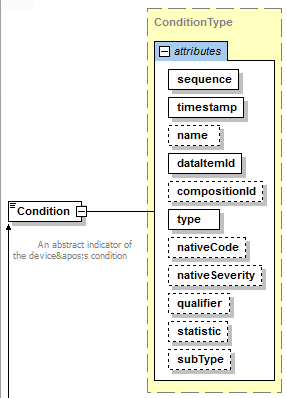
\includegraphics[width=0.6\textwidth]{figures/condition-schema-diagram.png}
  \caption{Condition Schema Diagram}
  \label{fig:condition-schema-diagram}
\end{figure}
\FloatBarrier

\subsubsection{Attributes for Condition}

\tbl{attributes-for-condition} defines the attributes used to provide additional information for a \gls{condition} XML element.


\tabulinesep = 5pt
\begin{longtabu} to \textwidth {
    |l|X[3l]|X[0.75l]|}
\caption{Attributes for Condition} \label{table:attributes-for-condition} \\

\hline
Attribute & Description & Occurrence \\
\hline
\endfirsthead

\hline
\multicolumn{3}{|c|}{Continuation of Table \ref{table:attributes-for-condition}}\\
\hline
Attribute & Description & Occurrence \\
\hline
\endhead

\gls{sequence} 
&
A number representing the sequential position of an occurrence of the
\gls{condition} in the data buffer of an MTConnect Agent.
\newline \gls{sequence} is a required attribute.
\newline \gls{sequence} \MUST have a value represented as an unsigned 64-bit value from 1 to $2^{64}-1$.
&
1 \\
\hline

\gls{timestamp} 
&
The most accurate time available to a piece of equipment that represents the point in time that the data reported for the \gls{condition} was measured.
\newline \gls{timestamp} is a required attribute.
&
1 \\
\hline

\gls{name} 
&
The name of the \gls{condition} element.
\newline \gls{name}  is an optional attribute.
\newline \gls{name}  \MUST match the \gls{name}  attribute of the \gls{dataitem} element defined in the \gls{mtconnectdevices} document that the \gls{condition}
element represents.
\newline An \gls{nmtoken} XML type. 
&
0..1 \\
\hline

\gls{dataitemid} 
&
The unique identifier for the\gls{condition} element.
\newline \gls{dataitemid} is a required attribute.
\newline \gls{dataitemid} \MUST match the id attribute of the \gls{dataitem}
element defined in the \gls{mtconnectdevices} document that the
\gls{condition} element represents. 
&
1 \\
\hline

\gls{type} 
&
An identifier of the \gls{type} of fault represented by the \gls{condition} element.
\newline \gls{type} is a required attribute.
\newline \gls{type} \MUST match the \gls{type} attribute of the \gls{dataitem} element defined in the \gls{mtconnectdevices} document that this \gls{condition} element represents. 
&
1 \\
\hline

\gls{nativecode}
&
The native code (usually an alpha-numeric value) generated by the
controller of a piece of equipment providing a reference identifier for a \gls{condition}.
\newline \gls{nativecode} is an optional attribute.
\newline This is the same information an operator or maintenance personnel may see as a reference code designating a specific fault code provided by the piece of equipment. 
&
0..1 \\
\hline

\gls{nativeseverity}
&
If the piece of equipment designates a severity level to a fault,
\gls{nativeseverity} reports that severity information to a client
software application.
\newline \gls{nativeseverity} is an optional attribute.
&
0..1 \\
\hline

\gls{qualifier}
&
\gls{qualifier} provides additional information regarding a \gls{fault state} associated with the measured value of a process variable.
\newline \gls{qualifier} is an optional attribute.
\newline \gls{qualifier} defines whether the \gls{fault state} represented by the \gls{condition} indicates a measured value that is above or below an expected value of a process variable.
\newline If the \gls{fault state} represents a measured value that is greater than the expected value for the process variable, \gls{qualifier} \MUST report a value of \gls{high}.
\newline If the \gls{fault state} represents a measured value that is less than the expected value for the process variable, \gls{qualifier} \MUST report a value of \gls{low}. 
&
0..1 \\
\hline

\gls{statistic}
&
\gls{statistic} provides additional information describing the meaning of the \gls{condition} element.
\newline \gls{statistic} is an optional attribute.
\newline \gls{statistic} \MUST match the \gls{statistic} attribute of the \gls{dataitem} element defined in the \gls{mtconnectdevices} document that this \gls{condition} element represents. 
&
0..1 \\
\hline

\gls{subtype} 
&
\gls{subtype} provides additional information describing the meaning of the \gls{condition} element.
\newline \gls{subtype} is an optional attribute.
\newline \gls{subtype} \MUST match the \gls{subtype} attribute of the \gls{dataitem} element defined in the \gls{mtconnectdevices} document that this \gls{condition} element represents. 
&
0..1 \\
\hline

\gls{compositionid}
&
The identifier of the \gls{composition} element defined in the
\gls{mtconnectdevices} document associated with the data reported for the \gls{condition} element.
\newline \gls{compositionid} is an optional attribute.
&
0..1 \\
\hline

\gls{xs:lang} 
&
An optional attribute that specifies the language of the \gls{cdata} returned for the \gls{condition}.
\newline Refer to IETF RFC 4646 (http://www.ietf.org/rfc/rfc4646.txt) or successor for a full definition of the values for this attribute.
\newline \gls{xs:lang} does not appear in the schema diagram.
&
0..1 \\
\hline

\end{longtabu}

\paragraph{qualifier Attribute for Condition}\mbox{}

Many \gls{condition} elements report the \gls{fault state} associated with the measured value of a process variable.

\gls{qualifier} provides an indication whether the measured value is above or below an expected value of a process variable.

As an example, a \gls{condition} element with a \gls{type} attribute of \gls{amperage sample} may differentiate between a higher than expected amperage and a lower than expected amperage by using the \gls{qualifier} attribute.

When a \gls{qualifier} of either \gls{high} or \gls{low} is used with \gls{fault} and \gls{warning}, the \glspl{fault state} can be differentiated as follows:

\quad \gls{fault},\gls{low}

\quad \gls{warning},\gls{low}

\quad \gls{normal}

\quad \gls{warning},\gls{high}

\quad \gls{fault},\gls{high}

\lst{example-of-condition-using-qualifier} is an example of an XML element representing \gls{condition} using \gls{qualifier}:

\begin{lstlisting}[firstnumber=1,escapechar=|,%
    caption={Example of a Condition Element using qualifier},label={lst:example-of-condition-using-qualifier}]
<Warning type="FILL_LEVEL" dataItemId="pm6" 
    qualifier="HIGH" sequence="32" 
    timestamp="2009-11-13T08:32:18">...</Warning>
\end{lstlisting}

\subsubsection{Valid Data Value for Condition}

\gls{condition} elements reported in an \gls{mtconnectstreams} XML document \may provide a value in the \gls{cdata} of the \gls{data entity} when additional information regarding the \gls{fault state} is available.

A \gls{valid data value} for the \gls{cdata} included in a \gls{condition} element \may be any text string.   A \gls{valid data value} is not required to be reported for a \gls{condition} category \gls{data entity}.  The \gls{fault state} and the attributes provided in a \gls{condition} element \may be sufficient to fully describe the \gls{data entity}.

The \gls{valid data value} reported as \gls{cdata} for a \gls{condition} element \must be formatted as part of the content between the element tags in the XML element representing that \gls{data entity}.  As an example, \gls{condition} elements are formatted as shown in \lst{example-of-cdata-for-condition}:

\begin{lstlisting}[firstnumber=1,escapechar=|,%
    caption={Example of CDATA for Condition},label={lst:example-of-cdata-for-condition}]
<Warning type="FILL_LEVEL" dataItemId="pm6" 
    qualifier="HIGH" sequence="32" timestamp=
    "2009-11-13T08:32:18">Fill Level on Tank
    #12 is reaching a high level</Warning>
\end{lstlisting}

In this example, the "Fill Level on Tank \#12 is reaching a high level" is the \gls{cdata} for the \gls{data entity}.

\subsection{Unavailability of Fault State for Condition}\label{sec:Unavailability of Fault State for Condition}

When an \gls{agent} cannot determine a valid \gls{fault state} for a \gls{condition} element, it \must report the \gls{element name} for the \gls{data entity} as Unavailable.

\lst{example-of-condition-when-fault-state-is-unavailable} demonstrates how an \gls{agent} reports a \gls{condition} category \gls{data entity} when it is unable to determine a valid \gls{fault state}:

\begin{lstlisting}[firstnumber=1,escapechar=|,%
    caption={Example of Condition when Fault State is UNAVAILABLE},label={lst:example-of-condition-when-fault-state-is-unavailable}]
<Unavailable type="MOTION_PROGRAM" dataItemId="cc2" 
    sequence="25" timestamp=
    "2009-11-13T08:32:18">...</Unavailable>
<Unavailable type="COMMUNICATIONS" dataItemId="cc1" 
    sequence="26" timestamp=
    "2009-11-13T08:32:18">...</Unavailable>
<Unavailable type="LOGIC_PROGRAM" dataItemId="cc3"
    sequence="28" timestamp=
    "2009-11-13T08:32:18">...</Unavailable>
<Unavailable type="LOGIC_PROGRAM" dataItemId="pm6"
    sequence="32" timestamp=
    "2009-11-13T08:32:18">...</Unavailable>
\end{lstlisting}

\section{Listing of Data Entities}\label{sec:Listing of Data Entities}

\glspl{data entity} that report data in \gls{mtconnectstreams} documents are represented by \gls{sample}, \gls{event}, or \gls{condition} elements based upon the \gls{category} and \gls{type} attributes defined for the corresponding \gls{dataitem} XML element in the \gls{mtconnectdevices} document.

Each \gls{data entity} in the \gls{mtconnectstreams} document has an \gls{element name}, as defined in the following sections, based upon the corresponding \gls{category} attribute defined for that \gls{dataitem} element in the \gls{mtconnectdevices} document.

\subsection{Sample Element Names}\label{sec:Sample Element Names}

\tbl{element-names-sample} lists the XML elements that can be placed in the \gls{samples} container of the \gls{componentstream} element.

The \tbl{element-names-sample} shows both the \gls{type} attribute for each \gls{sample category} category \gls{dataitem} element as defined in the \gls{mtconnectdevices} document and the corresponding \gls{element name} for the \gls{data entity} that \must be reported as a \gls{sample} element in the \gls{mtconnectstreams} document. 


\tabulinesep = 5pt
\begin{longtabu} to \textwidth {
    |X[2.5l]|X[3l]|X[3l]|}
\caption{Element Names for Sample} 
\label{table:element-names-sample} \\

\hline
DataItem Type & Element Name & Description\\
\hline
\endfirsthead

\hline
\multicolumn{3}{|c|}{Continuation of Table \ref{table:element-names-sample}}\\
\hline
DataItem Type & Element Name & Description\\
\hline
\endhead


\gls{acceleration sample}
&
\glselementname{acceleration sample}
&
\glsentrydesc{acceleration sample}
\newline \glselementname{acceleration sample} \MUST be reported in units of \glsunits{acceleration sample}.
\\ \hline 

\gls{accumulatedtime sample}
&
\glselementname{accumulatedtime sample}
&
\glsentrydesc{accumulatedtime sample}
\newline \glselementname{accumulatedtime sample} \MUST be reported in units of \glsunits{acceleration sample}.
\newline \DEPRECATIONWARNING:  May be deprecated in the future. Recommend using \glselementname{processtimer sample} and \glselementname{equipmenttimer sample}.
\\ \hline 

\gls{amperage sample}
&
\glselementname{amperage sample}
& \glsentrydesc{amperage sample}
\newline Subtypes of \glselementname{amperage sample} are \gls{alternating subtype}, \gls{direct subtype}, \gls{actual subtype}, and  \gls{target subtype}. 
\newline If a \gls{subtype} is not specified, the reported value for the data \MUST default to the \gls{subtype} of \gls{actual subtype}.
\newline \glselementname{amperage sample} \MUST be reported in units of \glsunits{amperage sample}.
\\ \hline 

\gls{angle sample}
&
\glselementname{angle sample} 
&
\glsentrydesc{angle sample}
\newline Subtypes of \glselementname{angle sample} are \gls{actual subtype} and \gls{commanded subtype}.
\newline If a \gls{subtype} is not specified, the reported value for the data \MUST default to the \gls{subtype} of \gls{actual subtype}.
\newline \glselementname{angle sample} \MUST be reported in units of \glsunits{angle sample}.
\\ \hline 

\gls{angularacceleration sample}
&
\glselementname{angularacceleration sample} 
&
\glsentrydesc{angularacceleration sample}
\newline \glselementname{angularacceleration sample} \MUST be reported in
units of \glsunits{angularacceleration sample}.
\\ \hline 

\gls{angularvelocity sample}
&
\glselementname{angularvelocity sample}
& \glsentrydesc{angularvelocity sample}
\newline \glselementname{angularvelocity sample} \MUST be reported in units
of \glsunits{angularvelocity sample}.
\\ \hline 

\gls{axisfeedrate sample}
&
\glselementname{axisfeedrate sample}
& \glsentrydesc{axisfeedrate sample}
\newline Subtypes of \glselementname{axisfeedrate sample} are \gls{actual subtype}, \gls{commanded subtype}, \gls{jog subtype}, \gls{programmed subtype}, and \gls{rapid subtype}.
\newline If a \gls{subtype} is not specified, the reported value
for the data \MUST default to the \gls{subtype} of \gls{programmed subtype}.
\newline \glselementname{axisfeedrate sample} \MUST be reported in units of
\glsunits{axisfeedrate sample}.
\\ \hline 

\gls{clocktime sample}
&
\glselementname{clocktime sample}
& \glsentrydesc{clocktime sample}
\newline \glselementname{clocktime sample} \must be reported in W3C ISO 8601 format of \glsunits{clocktime sample}.
\\ \hline 

\gls{concentration sample}
&
\glselementname{concentration sample}
&
\glsentrydesc{concentration sample}
\newline \glselementname{concentration sample} \MUST be reported in units of \glsunits{concentration sample}.
\\ \hline 

\gls{conductivity sample}
&
\glselementname{conductivity sample}
&
\glsentrydesc{conductivity sample}
\newline \glselementname{conductivity sample} \MUST be reported in units of \glsunits{conductivity sample}.
\\ \hline 

\gls{displacement sample}
&
\glselementname{displacement sample}
&
\glsentrydesc{displacement sample}
\newline \glselementname{displacement sample} \MUST be reported in units of \glsunits{displacement sample}.
\\ \hline 

\gls{electricalenergy sample}
&
\glselementname{electricalenergy sample}
&
\glsentrydesc{electricalenergy sample}
\newline \glselementname{electricalenergy sample} \MUST be reported in units of \glsunits{electricalenergy sample}.
\\ \hline 

\gls{equipmenttimer sample}
&
\glselementname{equipmenttimer sample}
&
\glsentrydesc{equipmenttimer sample}
\newline Subtypes of \glselementname{equipmenttimer sample} are \gls{loaded subtype}, \gls{working subtype}, \gls{operating subtype}, \gls{powered subtype}, and \gls{delay subtype}.
\newline A \gls{subtype} \MUST always be specified.
\newline \glselementname{equipmenttimer sample} \MUST be reported in units of \glsunits{equipmenttimer sample}.
\\ \hline 

\gls{filllevel sample}
&
\glselementname{filllevel sample}
&
\glsentrydesc{filllevel sample}
\newline \glselementname{filllevel sample} \MUST be reported in units of \glsunits{filllevel sample}.
\\ \hline 

\gls{flow sample}
& 
\glselementname{flow sample}
&
\glsentrydesc{flow sample}
\newline \glselementname{flow sample} \MUST be reported in units of \glsunits{flow sample}.
\\ \hline 

\gls{frequency sample}
&
\glselementname{frequency sample}
&
\glsentrydesc{frequency sample}
\newline \glselementname{frequency sample} \MUST be reported in units of \glsunits{frequency sample}.
\\ \hline 

\gls{globalposition sample} & \glselementname{globalposition sample} & \glsentrydesc{globalposition sample} \\ \hline 

\gls{length sample}
&
\glselementname{length sample}
&
\glsentrydesc{length sample}
\newline Subtypes of \glselementname{length sample} are \gls{standard subtype},
\gls{remaining subtype}, and \gls{useable subtype}.
\newline If a \gls{subtype} is not specified, the reported value
for the data \MUST default to the \gls{subtype} of
\gls{remaining subtype}.
\newline \glselementname{length sample} \MUST be reported in units of \glsunits{length sample}.
\\ \hline 

\gls{level sample} & \glselementname{level sample} & \glsentrydesc{level sample} \\ \hline 

\gls{linearforce sample}
&
\glselementname{linearforce sample}
&
\glsentrydesc{linearforce sample}
\newline \glselementname{linearforce sample} \MUST be reported in units of \glsunits{linearforce sample}.
\\ \hline 

\gls{load sample}
&
\glselementname{load sample}
&
\glsentrydesc{load sample}
\newline \glselementname{load sample} \MUST be reported in units of \glsunits{load sample}.
\\ \hline 

\gls{mass sample}
&
\glselementname{mass sample}
&
\glsentrydesc{mass sample}
\newline \glselementname{mass sample} \MUST be reported in units of \glsunits{mass sample}.
\\ \hline 

\gls{pathfeedrate sample}
&
\glselementname{pathfeedrate sample}
&
\glsentrydesc{pathfeedrate sample}
\newline Subtypes of \glselementname{pathfeedrate sample} are \gls{actual subtype},
\gls{commanded subtype},\gls{jog subtype}, \gls{programmed subtype}, and \gls{rapid subtype}.
\newline If a \gls{subtype} is not specified, the reported value
for the data \MUST default to the \gls{subtype} of
\gls{programmed subtype}.
\newline \glselementname{pathfeedrate sample} \MUST be reported in units of \glsunits{pathfeedrate sample}.
\\ \hline 

\gls{pathposition sample}
&
\glselementname{pathposition sample}
&
A measured or calculated position of a control point reported by a piece of equipment expressed in \gls{work} coordinates. The coordinate system will revert to \gls{machine} coordinates if \gls{work} coordinates are not available. 
\newline Subtypes of \glselementname{pathposition sample} are \gls{actual subtype}, \gls{programmed subtype}, \gls{commanded subtype}, \gls{target subtype}, and \gls{probe subtype}. 
\newline If a \gls{subtype} is not specified, the reported value for the data \MUST default to the subtype of \gls{actual subtype}. \newline \glselementname{pathposition sample} \MUST be reported as a set of space-delimited floating-point numbers representing a point in 3-D space. The position of the control point \MUST be reported in units of \gls{millimeter} and listed in order of X, Y, and Z referenced to the coordinate system of the piece of equipment. \\
\hline 

\gls{pathposition sample}
(Continued)
&
\glselementname{pathposition sample}
&
An example of the value reported for \glselementname{pathposition sample} would be: 
\newline <PathPosition ...>10.123 55.232 100.981 </PathPosition> Where X = 10.123, Y = 55.232, and Z=100.981. 
\\ \hline

\gls{ph sample}
&
\glselementname{ph sample}
&
\glsentrydesc{ph sample}
\newline \glselementname{ph sample} \MUST be reported in units of \glsunits{ph sample}.
\\ \hline 

\gls{position sample}
&
\glselementname{position sample}
&
\glsentrydesc{position sample}
\newline Subtypes of \glselementname{position sample} are \gls{actual subtype},
\gls{commanded subtype}, \gls{programmed subtype}, and \gls{target subtype}.
\newline If a \gls{subtype} is not specified, the reported value
for the data \MUST default to the \gls{subtype} of
\gls{actual subtype}.
\newline When \glselementname{position sample} is provided representing a
measured value for the physical axes of the piece of equipment, the data \MUST be provided in \gls{machine} coordinates.
\newline When \glselementname{position sample} is provided representing a
logical or calculated position, the data \MUST be provided in \gls{work} coordinates and is associated with a \gls{path} element of the equipment controller.
\newline \glselementname{position sample} \MUST be reported in units of \glsunits{position sample}.
\\ \hline 

\gls{powerfactor sample}
&
\glselementname{powerfactor sample}
&
\glsentrydesc{powerfactor sample}
\newline \glselementname{powerfactor sample} \MUST be reported in units of \glsunits{powerfactor sample}.
\\ \hline 

\gls{pressure sample}
&
\glselementname{pressure sample}
&
\glsentrydesc{pressure sample}
\glsentrydesc{pressure sample}
\newline \glselementname{pressure sample} \MUST be reported in units of \glsunits{pressure sample}.
\\ \hline 

\gls{processtimer sample}
&
\glselementname{processtimer sample}
&
\glsentrydesc{processtimer sample}
\newline Subtypes of \glselementname{processtimer sample} are \gls{process subtype}, and \gls{delay subtype}.
\newline A \gls{subtype} \MUST always be specified.
\newline \glselementname{processtimer sample} \MUST be reported in units of \glsunits{processtimer sample}.
\\ \hline 

\gls{resistance sample}
&
\glselementname{resistance sample}
&
\glsentrydesc{resistance sample}
\newline \glselementname{resistance sample} \MUST be reported in units of \glsunits{resistance sample}.
\\ \hline 

\gls{rotaryvelocity sample}
&
\glselementname{rotaryvelocity sample}
&
\glsentrydesc{rotaryvelocity sample}
\newline Subtypes of \glselementname{rotaryvelocity sample} are \gls{actual subtype},
\gls{commanded subtype} and \gls{programmed subtype}.
\newline If a \gls{subtype} is not specified, the reported value
for the data \MUST default to the \gls{subtype} of
\gls{actual subtype}.
\newline \glselementname{rotaryvelocity sample} \MUST be reported in units of \glsunits{rotaryvelocity sample}.
\\ \hline 

\gls{soundlevel sample}
&
\glselementname{soundlevel sample}
&
\glsentrydesc{soundlevel sample}
\newline Subtypes of \glselementname{soundlevel sample} are \gls{noscale subtype},
\gls{ascale subtype}, \gls{bscale subtype}, \gls{cscale subtype} and \gls{dscale subtype}.
\newline If a \gls{subtype} is not specified, the reported value
for the data \MUST default to the \gls{subtype} of
\gls{noscale subtype}.
\newline \glselementname{soundlevel sample} \MUST be reported in units of \glsunits{soundlevel sample}.
\\ \hline 

\gls{spindlespeed sample} & \glselementname{spindlespeed sample} & \glsentrydesc{spindlespeed sample} \\ \hline 

\gls{strain sample}
&
\glselementname{strain sample}
&
\glsentrydesc{strain sample}
\newline \glselementname{strain sample} \MUST be reported in units of \glsunits{strain sample}.
\\ \hline 

\gls{temperature sample}
&
\glselementname{temperature sample}
&
\glsentrydesc{temperature sample}
\newline \glselementname{temperature sample} \MUST be reported in units of \glsunits{temperature sample}.
\\ \hline 

\gls{tension sample}
&
\glselementname{tension sample}
&
\glsentrydesc{tension sample}
\newline \glselementname{tension sample} \MUST be reported in units of \glsunits{tension sample}.
\\ \hline 

\gls{tilt sample}
&
\glselementname{tilt sample}
&
\glsentrydesc{tilt sample}
\newline \glselementname{tilt sample} \MUST be reported in units of \glsunits{tilt sample}.
\\ \hline 

\gls{torque sample}
&
\glselementname{torque sample}
&
\glsentrydesc{torque sample}
\newline \glselementname{torque sample} \MUST be reported in units of \glsunits{torque sample}.
\\ \hline 

\gls{velocity sample}
&
\glselementname{velocity sample}
&
\glsentrydesc{velocity sample}
\newline When provided as the \glselementname{velocity sample} of the \gls{axes} \gls{component}, it represents the value of the velocity vector for all given axes, similar to \glselementname{pathfeedrate sample}.
\newline When provided as the \glselementname{velocity sample} of an individual \cfont{Axis} \gls{component}, it represents the value of the
velocity for that specific axis with no influence of the relative velocity of any other axes.
\newline \glselementname{velocity sample} \MUST be reported in units of \glsunits{velocity sample}.
\\ \hline 

\gls{viscosity sample}
&
\glselementname{viscosity sample}
&
\glsentrydesc{viscosity sample}
\newline \glselementname{viscosity sample} \MUST be reported in units of \glsunits{viscosity sample}.
\\ \hline 

\gls{voltampere sample}
&
\glselementname{voltampere sample}
&
\glsentrydesc{voltampere sample}
\newline \glselementname{voltampere sample} \MUST be reported in units of \glsunits{voltampere sample}.
\\ \hline 

\gls{voltamperereactive sample}
&
\glselementname{voltamperereactive sample}
&
\glsentrydesc{voltamperereactive sample} 
\newline \glselementname{voltamperereactive sample} \MUST be reported in units of \glsunits{voltamperereactive sample}.
\\ \hline 

\gls{voltage sample}
&
\glselementname{voltage sample}
&
\glsentrydesc{voltage sample}
\newline Subtypes of \glselementname{voltage sample} are \gls{alternating subtype}, \gls{direct subtype}, \gls{actual subtype} and \gls{target subtype}.
\newline If a \gls{subtype} is not specified, the reported value
for the data \MUST default to the \gls{subtype} of
\gls{actual subtype}.
\newline \glselementname{voltage sample} \MUST be reported in units of \glsunits{voltage sample}.
\\ \hline 

\gls{wattage sample}
&
\glselementname{wattage sample}
&
\glsentrydesc{wattage sample}
\newline Subtypes of \glselementname{wattage sample} are \gls{actual subtype} and \gls{target subtype}.
\newline If a \gls{subtype} is not specified, the reported value
for the data \MUST default to the \gls{subtype} of
\gls{actual subtype}.
\newline \glselementname{wattage sample} \MUST be reported in units of \glsunits{wattage sample}.
\\ \hline 



\DIFaddbegin \DIFadd{\gls{volumespatial sample}
}&
\DIFadd{\glselementname{volumespatial sample}
}&
\DIFadd{The geometric volume of an object or container.
}\newline \DIFadd{Subtypes of \glselementname{volumespatial sample} are \gls{actual subtype} and \gls{consumed subtype}.
}\newline \DIFadd{If a \gls{subtype} is not specified, the reported value for the data \MUST default to the subtype of \gls{actual subtype}.
}\newline \DIFadd{\glselementname{volumespatial sample} \MUST be reported in units of \gls{cubicmillimeter}. }\\
\hline

\DIFadd{\gls{volumefluid sample}
}&
\DIFadd{\glselementname{volumefluid sample}
}&
\DIFadd{The fluid volume of an object or container.
}\newline \DIFadd{Subtypes of \glselementname{volumefluid sample} are \gls{actual subtype} and \gls{consumed subtype}.
}\newline \DIFadd{If a \gls{subtype} is not specified, the reported value for the data \MUST default to the subtype of \gls{actual subtype}.
}\newline \DIFadd{\glselementname{volumefluid sample} \MUST be reported in units of \gls{milliliter}. }\\
\hline

\DIFadd{\gls{capacityspatial sample}
}&
\DIFadd{\glselementname{capacityspatial sample}
}&
\DIFadd{The geometric capacity of an object or container.
}\newline \DIFadd{\glselementname{capacityspatial sample} \MUST be reported in units of \gls{cubicmillimeter}. }\\
\hline

\DIFadd{\gls{capacityfluid sample}
}&
\DIFadd{\glselementname{capacityfluid sample}
}&
\DIFadd{The fluid capacity of an object or container.
}\newline \DIFadd{\glselementname{capacityfluid sample} \MUST be reported in units of \gls{milliliter}. }\\
\hline

\DIFadd{\gls{density sample}
}&
\DIFadd{\glselementname{density sample}
}&
\DIFadd{The volumetric mass of a material per unit volume of that material.
}\newline \DIFadd{\glselementname{density sample} \MUST be reported in units of \gls{milligrampercubicmillimeter}. }\\
\hline

\DIFadd{\gls{depositionvolume sample}
}&
\DIFadd{\glselementname{depositionvolume sample}
}&
\DIFadd{The spatial volume of material deposited in an additive manufacturing process.
}\newline \DIFadd{Subtypes of \glselementname{depositionvolume sample} are \gls{actual subtype} and \gls{commanded subtype}.
}\newline \DIFadd{If a \gls{subtype} is not specified, the reported value for the data \MUST default to the subtype of \gls{actual subtype}.
}\newline \DIFadd{\glselementname{depositionvolume sample} \MUST be reported in units of \gls{cubicmillimeter}. }\\
\hline

\DIFadd{\gls{depositionratevolumetric sample}
}&
\DIFadd{\glselementname{depositionratevolumetric sample}
}&
\DIFadd{The rate at which a spatial volume of material is deposited in an additive manufacturing process.
}\newline \DIFadd{Subtypes of \glselementname{depositionratevolumetric sample} are \gls{actual subtype} and \gls{commanded subtype}.
}\newline \DIFadd{If a \gls{subtype} is not specified, the reported value for the data \MUST default to the subtype of \gls{actual subtype}.
}\newline \DIFadd{\glselementname{depositionratevolumetric sample} \MUST be reported in units of \gls{cubicmillimeterpersecond}. }\\
\hline

\DIFadd{\gls{depositionaccelerationvolumetric sample}
}&
\DIFadd{\glselementname{depositionaccelerationvolumetric sample}
}&
\DIFadd{The rate of change in spatial volume of material deposited in an additive manufacturing process.
}\newline \DIFadd{Subtypes of \glselementname{depositionaccelerationvolumetric sample} are \gls{actual subtype} and \gls{commanded subtype}.
}\newline \DIFadd{If a \gls{subtype} is not specified, the reported value for the data \MUST default to the subtype of \gls{actual subtype}.
}\newline \DIFadd{\glselementname{depositionaccelerationvolumetric sample} \MUST be reported in units of \gls{cubicmillimeterpersecondsquared}. }\\
\hline

\DIFadd{\gls{depositionmass sample}
}&
\DIFadd{\glselementname{depositionmass sample}
}&
\DIFadd{The mass of the material deposited in an additive manufacturing process.
}\newline \DIFadd{Subtypes of \glselementname{depositionmass sample} are \gls{actual subtype} and \gls{commanded subtype}.
}\newline \DIFadd{If a \gls{subtype} is not specified, the reported value for the data \MUST default to the subtype of \gls{actual subtype}.
}\newline \DIFadd{\glselementname{depositionmass sample} \MUST be reported in units of \gls{milligram}. }\\
\hline

\DIFadd{\gls{depositiondensity sample}
}&
\DIFadd{\glselementname{depositiondensity sample}
}&
\DIFadd{The density of the material deposited in an additive manufacturing process per unit of volume.
}\newline \DIFadd{Subtypes of \glselementname{depositiondensity sample} are \gls{actual subtype} and \gls{commanded subtype}.
}\newline \DIFadd{If a \gls{subtype} is not specified, the reported value for the data \MUST default to the subtype of \gls{actual subtype}.
}\newline \DIFadd{\glselementname{depositiondensity sample} \MUST be reported in units of \gls{milligrampercubicmillimeter}. }\\
\hline

\DIFadd{\gls{cuttingspeed sample}
}&
\DIFadd{\glselementname{cuttingspeed sample}
}&
\DIFadd{The speed difference (relative velocity) between the cutting mechanism and the surface of the workpiece it is operating on.
}\newline \DIFadd{Subtypes of \gls{cuttingspeed sample} are \gls{actual subtype}, \gls{commanded subtype}, and \gls{programmed subtype}.
}\newline \DIFadd{If no \gls{subtype} is specified, the reported value must default to \gls{programmed subtype}.
}\newline \DIFadd{\glselementname{cuttingspeed sample} is reported in units of \gls{millimeterpersecond}. }\\
\hline

\DIFadd{\gls{pathfeedrateperrevolution sample}
}&
\DIFadd{\glselementname{pathfeedrateperrevolution sample}
}&
\DIFadd{The feedrate for the axes, or a single axis.
}\newline \DIFadd{\glselementname{pathfeedrateperrevolution sample} is reported in units of \gls{millimeterperrevolution}.
}\newline \DIFadd{Subtypes of \glselementname{pathfeedrateperrevolution sample} are \gls{actual subtype}, \gls{commanded subtype}, and \gls{programmed subtype}. }\\
\hline\DIFaddend \end{longtabu}

\begin{note}
Note: The \gls{sample} response format \must be extended when the \gls{representation} attribute for the data item is \gls{timeseries representation}.  See \sect{Response for SAMPLE category DataItem Elements with a representation Attribute of TIME_SERIES} for details on extending the response format.
\end{note}

\subsection{Event Element Names}
\label{sec:Event Element Names}

\tbl{element-names-event} lists the XML elements that can be placed in the \gls{events} container of the \gls{componentstream} element.

The \tbl{element-names-sample} shows both the \gls{type} for each \gls{event category} category \gls{dataitem} element defined in the \gls{mtconnectdevices} document and the corresponding \gls{element name} for the \gls{data entity} that \must be reported as an \gls{event} element in the \gls{mtconnectstreams} document.

The table also defines the \gls{valid data value} for those \gls{event} \gls{type} data items where the reported values are restricted to a \gls{controlled vocabulary}.


\tabulinesep = 5pt
\begin{longtabu} to \textwidth {
    |X[2l]|X[3.5l]|X[3l]|}
\caption{Element Names for Event} 
\label{table:element-names-event} \\

\hline
DataItem Type & Element Name & Description\\
\hline
\endfirsthead

\hline
\multicolumn{3}{|c|}{Continuation of Table \ref{table:element-names-event}}\\
\hline
DataItem Type & Element Name & Description\\
\hline
\endhead

\gls{activeaxes event}
&
\glselementname{activeaxes event}
&
\glsentrydesc{activeaxes event}
\newline The \gls{valid data value} reported \SHOULD be a space-delimited set of axes names. The names returned \SHOULD match the \gls{name} attribute of the \gls{linear} or \gls{rotary} \glspl{structural element} defined in the \gls{mtconnectdevices} document that this \gls{event} element represents. If \gls{name} is not available, \gls{nativename} \MUST be returned to identify the \gls{linear} or \gls{rotary} \glspl{structural element}.
\newline For example:
\newline \tab \cfont{<ActiveAxes ...>X Y Z W S</ActiveAxes>}
\newline where X, Y, Z, W, and S are the \gls{nativename} attributes of the \glspl{structural element}. 
\newline If it is not specified elsewhere in the \gls{mtconnectdevices} document, it \MUST be assumed that all of the axes are associated with the \gls{path} component.
\\ \hline 

\gls{actuatorstate event}
&
\glselementname{actuatorstate event}
&
\glsentrydesc{actuatorstate event}
\newline \glspl{valid data value}:
\newline \tab \gls{active value}: The actuator is operating
\newline \tab \gls{inactive value}: The actuator is not operating 
\\ \hline 

\gls{alarm event} & \glselementname{alarm event} & \glsentrydesc{alarm event} \\ \hline 

\gls{availability event}
&
\glselementname{availability event}
&
\glsentrydesc{availability event}
\newline \glselementname{availability event} \MUST be provided for each \gls{device} \gls{structural element} and \MAY be provided for any other \gls{structural element}.
\newline \glspl{valid data value}:
\newline \tab \gls{available value}: The \gls{structural element} is active and capable of providing data.
\newline \tab \gls{available value}: The \gls{structural element} is either inactive or not capable of providing data.
\\ \hline 

\gls{axiscoupling event}
&
\glselementname{axiscoupling event}
&
\glsentrydesc{axiscoupling event}
\newline The coupling of the axes \MUST be viewed from the
perspective of a specified axis. Therefore, a
\gls{master value} coupling indicates that this axis is the
master for the \gls{coupledaxes event}.
\newline \glselementname{axiscoupling event} \MUST be provided for each axis
element associated with a set of axes defined by the
\gls{coupledaxes event} data item element defined in the
\gls{mtconnectdevices} document.
\newline \glspl{valid data value}:
\newline \tab \gls{tandem value}: The axes are physically connected to
each other and operate as a single unit.
\newline \tab \gls{synchronous value}: The axes are not physically
connected to each other but are operating together in
lockstep.
\newline \tab \gls{master value}: The axis is the master of the
\glselementname{coupledaxes event}
\newline \tab \gls{slave value}: The axis is a slave to the
\glselementname{coupledaxes event}
\\ \hline 

\gls{axisfeedrateoverride event}
&
\glselementname{axisfeedrateoverride event}
&
\glsentrydesc{axisfeedrateoverride event}
\newline The value provided for
\glselementname{axisfeedrateoverride event} is expressed as a
percentage of the designated feedrate for the axis.
\newline Subtypes of \glselementname{axisfeedrateoverride event} are \gls{jog subtype},
\gls{programmed subtype}, and \gls{rapid subtype}.
\newline If a \gls{subtype} is not specified, the reported value
for the data \MUST default to the \gls{subtype} of
\gls{programmed subtype}.
\newline The \gls{valid data value} \MUST be a floating-point
number.
\\ \hline 

\gls{axisinterlock event}
&
\glselementname{axisinterlock event}
&
\glsentrydesc{axisinterlock event}
\newline \glspl{valid data value}:
\newline \gls{active value}: The axis lockout function is activated,
power has been removed from the axis, and the axis
is allowed to move freely.
\newline \gls{inactive value}: The axis lockout function has not
been activated, the axis may be powered, and the
axis is capable of being controlled by another
component.
\\ \hline 

\gls{axisstate event}
&
\glselementname{axisstate event}
&
\glsentrydesc{axisstate event}
\newline \glspl{valid data value}:
\newline \tab \gls{home value}: The axis is in its home position.
\newline \tab \gls{travel value}: The axis is in motion
\newline \tab \gls{parked value}: The axis has been moved to a fixed
position and is being maintained in that position
either electrically or mechanically. Action is
required to release the axis from this position.
\newline \tab \gls{stopped value}: The axis is stopped
\\ \hline 

\gls{block event}
&
\glselementname{block event}
&
\glsentrydesc{block event}
\newline \glselementname{block event} \MUST include the entire expression for a line of program code, including all parameters
\newline The \gls{valid data value} \MUST be a text string.
\\ \hline 

\gls{blockcount event}
&
\glselementname{blockcount event}
&
\glsentrydesc{blockcount event}
\newline The \gls{valid data value} \MUST be an integer.
\\ \hline 

\gls{chuckinterlock event}
&
\glselementname{chuckinterlock event}
&
\glsentrydesc{chuckinterlock event}
\newline A \gls{chuck} component or composition element may
be controlled by more than one type of
\glselementname{chuckinterlock event} function. When the
\newline \glselementname{chuckinterlock event} function is provided by an
operator controlled interlock that can inhibit the
ability to initiate an unclamp action of an
electronically controlled chuck, this
\newline \glselementname{chuckinterlock event} function \SHOULD be further
characterized by specifying a \gls{subtype} of
\gls{manualunclamp subtype}.
\newline \glspl{valid data value}:
\newline \tab \gls{active value}: The chuck cannot be unclamped
\newline \tab \gls{inactive value}: The chuck can be unclamped.
\\ \hline 

\gls{chuckstate event}
&
\glselementname{chuckstate event}
&
\glsentrydesc{chuckstate event}
\newline \glspl{valid data value}:
\newline \tab \gls{open value}: The \gls{chuck} component or composition
element is open to the point of a positive
confirmation
\newline \tab \gls{closed value}: The \gls{chuck} component or
composition element is closed to the point of a
positive confirmation
\newline \tab \gls{unlatched value}: The \gls{chuck} component or
composition element is not closed to the point of a
positive confirmation and not open to the point of a
positive confirmation. It is in an intermediate
position.
\\ \hline 

\gls{code event} & \glselementname{code event} & \glsentrydesc{code event} \\ \hline 

\gls{compositionstate event}
&
\glselementname{compositionstate event}
&
\glsentrydesc{compositionstate event}
\newline Subtypes of \glselementname{compositionstate event} are \gls{action subtype}, \gls{lateral subtype}, \gls{motion subtype}, \gls{switched subtype}, and \gls{vertical subtype}.
\newline A \gls{subtype} \MUST be provided.
\newline \glspl{valid data value} for \gls{subtype} \gls{action subtype} are:
\newline \tab \gls{active value}: The \gls{composition} element is
operating
\newline \tab \gls{inactive value}: The \gls{composition} element is not
operating.
\newline \glspl{valid data value} for \gls{subtype} \gls{lateral subtype} are:
\newline \tab \gls{right value} : The position of the \gls{composition} 
element is oriented to the right to the point of a
positive confirmation
\newline \tab \gls{left value} : The position of the \gls{composition} 
element is oriented to the left to the point of a
positive confirmation
\\ \hline

\gls{compositionstate event}
\newline (Continued)
&
\glselementname{compositionstate event}
&
\tab \gls{transitioning value} : The position of the
\gls{composition} element is not oriented to the right
to the point of a positive confirmation and is not
oriented to the left to the point of a positive
confirmation. It is in an intermediate position.
\newline \glspl{valid data value} for \gls{subtype} \gls{motion subtype} are:
\newline \tab \gls{open value}: The position of the \gls{composition} 
element is open to the point of a positive
confirmation
\newline \tab \gls{closed value}: The position of the \gls{composition} 
element is closed to the point of a positive
confirmation
\newline \tab \gls{unlatched value}: The position of the
\gls{composition} element is not open to the point of
a positive confirmation and is not closed to the point
of a positive confirmation. It is in an intermediate
position.
\\ \hline

\gls{compositionstate event}
\newline (Continued)
&
\glselementname{compositionstate event}
&
\glspl{valid data value} for \gls{subtype} \gls{switched subtype} are:
\newline \tab \gls{on value} : The activation state of the \gls{composition} 
element is in an \gls{on value}  condition, it is operating, or it is
powered.
\newline \tab \gls{off value} : The activation state of the \gls{composition}
element is in an \gls{off value}  condition, it is not operating,
or it is not powered.
\glspl{valid data value} for \gls{subtype} \gls{vertical subtype} are:
\newline \tab \gls{up value} : The position of the \gls{composition} element
is oriented in an upward direction to the point of a
positive confirmation
\newline \tab \gls{down value} : The position of the \gls{composition} 
element is oriented in a downward direction to the
point of a positive confirmation
\newline \tab \gls{transitioning value} : The position of the
\gls{composition} element is not oriented in an
upward direction to the point of a positive
confirmation and is not oriented in a downward
direction to the point of a positive confirmation. It
is in an intermediate position.
\\ \hline

\gls{controllermode event}
&
\glselementname{controllermode event}
&
The current operating mode of the \gls{controller} component.
\DIFaddend \newline \glspl{valid data value}:
\newline 	\DIFdelbegin %DIFDELCMD < \tab %%%
\DIFdelend \DIFaddbegin \DIFadd{\tab}\DIFaddend \gls{automatic value}: The controller is configured to automatically execute a program. 
\newline 	\DIFdelbegin %DIFDELCMD < \tab %%%
\DIFdelend \DIFaddbegin \DIFadd{\tab}\DIFaddend \gls{manual value}: The controller is not executing an active program. It is capable of receiving instructions from an external source - typically an operator. The controller executes operations based on the instructions received from the external source. 
\newline 	\DIFdelbegin %DIFDELCMD < \tab %%%
\DIFdelend \DIFaddbegin \DIFadd{\tab}\DIFaddend \gls{manualdatainput value}: The operator can enter a series of operations for the controller to perform. The controller will execute this specific series of operations and then stop. 
\\ \hline

\gls{controllermode event}
(continued)
&
\glselementname{controllermode event}
&
\newline 	\DIFdelbegin %DIFDELCMD < \tab %%%
\DIFdelend \DIFaddbegin \DIFadd{\tab}\DIFaddend \gls{semiautomatic value}: The controller is operating in \DIFdelbegin \DIFdel{a single cycle mode. It executes a single set of
instructions from an active program and then stops
until given a command to execute the next set of
instructions}\DIFdelend \DIFaddbegin \DIFadd{a mode that restricts the active program from processing it's next process step without operator intervention}\DIFaddend . 
\newline 	\DIFdelbegin %DIFDELCMD < \tab %%%
\DIFdelend \DIFaddbegin \DIFadd{\tab}\DIFaddend \gls{edit value}: The controller is currently functioning as a programming device and is not capable of executing an active program. \\
\hline 

\gls{controllermodeoverride event}
&
\glselementname{controllermodeoverride event}
&
\glsentrydesc{controllermodeoverride event}
\newline Subtypes of \glselementname{controllermodeoverride event} are \gls{dryrun subtype}, \gls{singleblock subtype}, \gls{machineaxislock subtype},
\gls{optionalstop subtype}, and \gls{toolchangestop subtype}.
\newline A \gls{subtype} \MUST always be specified.
\newline \glspl{valid data value}:
\newline \tab \gls{on value} : The indicator of the
\glselementname{controllermodeoverride event} is in the \gls{on value}  state
and the mode override is active.
\newline \tab \gls{off value} : The indicator of the
\glselementname{controllermodeoverride event} is in the \gls{off value}  state and the mode override is inactive
\\ \hline 

\gls{coupledaxes event}
&
\glselementname{coupledaxes event}
&
\glsentrydesc{coupledaxes event}
\newline Used in conjunction with \glselementname{axiscoupling event} to
describe how the \glselementname{coupledaxes event} relate to each
other.
\newline The \gls{valid data value} reported \SHOULD be a
space-delimited set of axes names. The names
returned \SHOULD match the name attribute of the
\gls{linear}  or \gls{rotary}  \glspl{structural element} defined in
the \gls{mtconnectdevices} document that this
\gls{event} element represents. If name is not
available, \gls{nativename} \MUST be returned to
identify the \gls{linear}  or \gls{rotary}  \glspl{structural element}.
\newline Example:
\newline \cfont{<CoupledAxes ...>Y1 Y2</CoupledAxes>}
\\ \hline 

\DIFadd{\gls{deviceuuid event}
}&
\DIFadd{\glselementname{deviceuuid event}
}&
\DIFadd{The identifier of another piece of equipment that is temporarily associated with a component of this piece of equipment to perform a particular function.
}\newline \DIFadd{\glspl{valid data value} are the value of the UUID attribute of the associated device - a NMTOKEN XML type. }\\
\hline

\gls{direction event}
&
\glselementname{direction event}
&
\glsentrydesc{direction event}
\newline Subtypes of \glselementname{direction event} are \gls{rotary subtype} and \gls{linear subtype}.
\newline A \gls{subtype} \MUST always be specified.
\glspl{valid data value} for \gls{subtype} \gls{rotary subtype} are:
\newline \tab \gls{clockwise value} : A \gls{rotary} type component is rotating in a clockwise fashion using the right-hand
rule.
\newline \tab \gls{counterclockwise value} : A \gls{rotary} type component is rotating in a counter clockwise
fashion using the right-hand rule.
\glspl{valid data value} for \gls{subtype} \gls{linear subtype} are:
\newline \tab \gls{positive value} : A \gls{linear} type component is moving in the direction of increasing position value
\newline \tab \gls{negative value} : A \gls{linear} type component is moving in the direction of decreasing position value
\\ \hline 

\gls{doorstate event}
&
\glselementname{doorstate event}
&
\glsentrydesc{doorstate event}
\newline \glspl{valid data value}:
\newline \tab \gls{open value}: The \gls{door}  is open to the point of a
positive confirmation
\newline \tab \gls{closed value}: The \gls{door}  is closed to the point of a
positive confirmation
\newline \tab \gls{unlatched value}: The \gls{door} is not closed to the
point of a positive confirmation and is not open to
the point of a positive confirmation. It is in an
intermediate position.
\\ \hline 

\gls{emergencystop event}
&
\glselementname{emergencystop event}
&
\glsentrydesc{emergencystop event}
\newline \glspl{valid data value}:
\newline \tab \gls{armed value} : The emergency stop circuit is complete
and the piece of equipment, component, or
composition element is allowed to operate.
\newline \tab \gls{triggered value} : The emergency stop circuit is open
and the operation of the piece of equipment,
component, or composition element is inhibited.
\\ \hline 

\gls{endofbar event}
&
\glselementname{endofbar event}
&
\glsentrydesc{endofbar event}
\newline Subtypes of \glselementname{endofbar event} are \gls{primary subtype} and \gls{auxiliary subtype}.
\newline If a \gls{subtype} is not specified, the reported value
for the data \MUST default to the \gls{subtype} of
\gls{primary subtype}.
\newline \glspl{valid data value}:
\newline \tab \gls{yes value} : The \glselementname{endofbar event} has been reached.
\newline \tab \gls{no value} : The \glselementname{endofbar event} has not been reached.
\\ \hline 

\gls{equipmentmode event}
&
\glselementname{equipmentmode event}
&
\glsentrydesc{equipmentmode event}
\newline Subtypes of \glselementname{equipmentmode event} are \gls{loaded subtype}, \gls{working subtype}, \gls{operating subtype}, and \gls{powered subtype}.
\newline A \gls{subtype} \MUST always be specified.
\newline \glspl{valid data value}:
\newline \tab \gls{on value} : The equipment is functioning in the mode
designated by the \gls{subtype}.
\newline \tab \gls{off value} : The equipment is not functioning in the
mode designated by the \gls{subtype}.
\\ \hline 

\gls{execution event}
&
\glselementname{execution event}
&
\glsentrydesc{execution event}
\newline \glspl{valid data value}:
\newline  \tab \gls{ready value} : The controller is ready to execute
instructions. It is currently idle.
\newline \gls{active value}: The controller is actively executing an
instruction.
\newline  \tab \gls{interrupted value} : The execution of the
controller's program has been suspended due to an
external signal. Action is required to resume
execution.
\newline 	\DIFadd{\tab \gls{wait}:  The execution of the controller's program is suspended while a secondary operation is executing or completing.  Execution will resume automatically once the secondary operation is completed.
}
\newline  \tab \gls{feedhold value} : Motion of the device has been
commanded to stop at its current position. The
controller remains able to execute instructions but
cannot complete the current set of instructions until
after motion resumes. The command to stop the
motion must be removed before execution can
resume. \\ \hline

\gls{execution event}
(Continued)
&
\glselementname{execution event}
&
\tab \gls{stopped value}: The execution of the controller's
program has been stopped in an unplanned manner
and execution of the program cannot be resumed
without intervention by an operator or external
signal.
\newline 	\DIFadd{\tab}\DIFaddend \gls{optionalstop value}:  The controller's program has been intentionally stopped using an M01 or similar command.  The program may be stopped at the designated location based upon the state of a secondary indication provided to the controller indicating whether the program execution must be stopped at this location or program execution should continue.
\newline 	\DIFdelbegin %DIFDELCMD < \tab %%%
\DIFdelend \DIFaddbegin \DIFadd{\tab}\DIFaddend \gls{programstopped value}:  The execution of the controller's program has been stopped by a command from within the program.   Action is required to resume execution.
\newline 	\DIFdelbegin %DIFDELCMD < \tab %%%
\DIFdelend \DIFaddbegin \DIFadd{\tab}\DIFaddend \gls{programcompleted value}:  The program has completed execution. \\
\hline 

\gls{functionalmode event}
&
\glselementname{functionalmode event}
&
\glsentrydesc{functionalmode event}
\newline Typically, the \glselementname{functionalmode event} \SHOULD be
associated with the \gls{device} \gls{structural element}, but
it \MAY be associated with any \gls{structural element}
in the XML document.
\newline \glspl{valid data value}:
\newline \tab \gls{production value} : The \gls{device} element or another
\gls{structural element} is currently producing product,
ready to produce product, or its current intended use
is to be producing product.
\newline \tab \gls{setup value} : The \gls{device} element or another
\gls{structural element} is not currently producing
product. It is being prepared or modified to begin
production of product.
\newline \tab \gls{teardown value} : The \gls{device} element or another
\gls{structural element} is not currently producing
product. Typically, it has completed the production
of a product and is being modified or returned to a
neutral state such that it may then be prepared to
begin production of a different product.
\\ \hline 

\gls{functionalmode event}
\newline (Continued)
&
\glselementname{functionalmode event}
&
\tab \gls{maintenance} : The \gls{device} element or
another \gls{structural element} is not currently
producing product. It is currently being repaired,
waiting to be repaired, or has not yet been returned
to a normal production status after maintenance has
been performed.
\newline \tab \gls{processdevelopment value} : The \gls{device}
element or another \gls{structural element} is being used
to prove-out a new process, testing of equipment or
processes, or any other active use that does not
result in the production of product.
\\ \hline 

\gls{hardness event}
&
\glselementname{hardness event}
&
\glsentrydesc{hardness event}
\newline Subtypes of \glselementname{hardness event} are \gls{rockwell subtype}, \gls{vickers subtype}, \gls{shore subtype}, \gls{brinell subtype}, \gls{leeb subtype}, and \gls{mohs subtype}.
\newline A \gls{subtype} \MUST always be specified.
\newline The \gls{valid data value} \MUST be a floating-point
number.
\\ \hline 

\gls{interfacestate event}
&
\glselementname{interfacestate event}
&
The current functional or operational state of an \gls{interface component} type element indicating whether the \gls{interface} is active or not currently functioning.
\newline \glspl{valid data value}:
\newline \tab \gls{enabled value}: The \gls{interface} is currently operational and performing as expected.
\newline \tab \gls{disabled value}: The Interface is currently not operational.
\newline When the \gls{interfacestate event} is \gls{disabled value}, the state of all data items that are specific for the \gls{interaction model} associated with that \gls{interface} \MUST be set to \gls{notready value}.
\\ \hline 

\gls{line event} & \glselementname{line event} & \glsentrydesc{line event} \\ \hline 

\gls{linelabel event}
&
\glselementname{linelabel event}
&
\glsentrydesc{linelabel event}
\newline The \gls{valid data value} \MUST be any text string.
\\ \hline 

\gls{linenumber event}
&
\glselementname{linenumber event}
&
\glsentrydesc{linenumber event}
\newline Subtypes of \glselementname{linenumber event} are \gls{absolute subtype} and \gls{incremental subtype}.
\newline A \gls{subtype} \MUST always be specified.
\newline The \gls{valid data value} \MUST be an integer.
\\ \hline 

\gls{material event}
&
\glselementname{material event}
&
\glsentrydesc{material event}
\newline The \gls{valid data value} \MUST be any text string.
\\ \hline 

\gls{message event}
&
\glselementname{message event}
&
\glsentrydesc{message event}
\newline The \gls{valid data value} \MUST be any text string.
\\ \hline 

\gls{operatorid event}
&
\glselementname{operatorid event}
&
\glsentrydesc{operatorid event}
\newline The \gls{valid data value} \MAY be any text string.
\newline \DEPRECATIONWARNING: May be
deprecated in the future. See USER below.
\\ \hline 

\gls{palletid event}
&
\glselementname{palletid event}
&
\glsentrydesc{palletid event}
\newline The \gls{valid data value} \MAY be any text string.
\\ \hline 

\gls{partcount}
&
\glselementname{partcount}
&
The current count of parts produced as represented by the \gls{controller} component.
\newline Subtypes of \glselementname{partcount} are \gls{all subtype}, \gls{good subtype}, \gls{bad subtype}, \gls{target subtype}, and \gls{remaining subtype}.
\newline \glselementname{partcount} will not be accumulated by an
\gls{agent} and \MUST only be supplied if
the \gls{controller}  provides the count.
\newline \glselementname{partcount} \MAY have a \gls{representation} of
\gls{discrete representation}. In this case, each occurrence of
\glselementname{partcount} in an \gls{mtconnectstreams}
document represents a unique count of parts or
product produced - it is not an accumulated count of
parts or product produced.
\newline The \gls{valid data value} \MUST be a floating-point
number, usually an integer.
\\ \hline 

\gls{partid event}
&
\glselementname{partid event}
&
\glsentrydesc{partid event}
\newline The \gls{valid data value} \MAY be any text string.
\\ \hline

\gls{partnumber event}
&
\glselementname{partnumber event}
&
An identifier of a part or product moving through the manufacturing process.
\newline The \gls{valid data value} \MUST be a text string. 
\newline \DIFadd{\DEPRECATIONWARNING: May be deprecated in the future. }\DIFaddend \\
\hline 

\gls{pathfeedrateoverride event}
&
\glselementname{pathfeedrateoverride event}
&
\glsentrydesc{pathfeedrateoverride event}
\newline The value provided for
\glselementname{pathfeedrateoverride event} is expressed as a
percentage of the designated feedrate for the path.
\newline Sub-types of \glselementname{pathfeedrateoverride event} are \gls{jog subtype}, \gls{programmed subtype}, and \gls{rapid subtype}.
\newline If a \gls{subtype} is not specified, the reported value
for the data \MUST default to the \gls{subtype} of
\gls{programmed subtype}.
\newline The \gls{valid data value} \MUST be a floating-point
number.
\\ \hline 

\gls{pathmode event}
&
\glselementname{pathmode event}
&
\glsentrydesc{pathmode event}
\newline \glspl{valid data value}:
\newline \tab \gls{independent value} : The path is operating
independently and without the influence of another
path.
\newline  \tab \gls{master value}: The path provides the reference motion
for a \gls{synchronous value} or \gls{mirror value}  type path to
follow. For non-motion type paths, the \gls{master value}
provides information or state values that influences
the operation of other paths
\newline  \tab \gls{synchronous value}: The axes associated with the
path are following the motion of the \gls{master value} type
path.
\newline  \tab \gls{mirror value} : The axes associated with the path are
mirroring the motion of the \gls{master value} path.
When \glselementname{pathmode event} is not specified, the operational
mode of the path \MUST be interpreted as
\gls{independent value} .
\\ \hline 

\gls{powerstate event}
&
\glselementname{powerstate event}
&
\glsentrydesc{powerstate event}
\newline Subtypes of \glselementname{powerstate event} are LINE and
CONTROL.
\newline When the \gls{subtype} is \gls{line subtype}, \glselementname{powerstate event}
represents the primary source of energy for a \gls{structural element}.
\newline When the \gls{subtype} is \gls{control subtype}, \glselementname{powerstate event} represents an enabling signal providing permission for the \gls{structural element} to perform its function(s).
\newline If a \gls{subtype} is not specified, the reported value
for the data \MUST default to the \gls{subtype} of \gls{line subtype}.
\\ \hline 

\gls{powerstate event}
\newline (Continued)
&
\glselementname{powerstate event}
&
\glspl{valid data value}:
\newline \tab \gls{on value} : The source of energy for a \gls{structural element} or the enabling signal providing permission for the
\gls{structural element} to perform its function(s) is
present and active.
\newline \tab \gls{off value} : The source of energy for a \gls{structural element} or the enabling signal providing permission
for the \gls{structural element} to perform its function(s)
is not present or is disconnected.
\newline \DEPRECATIONWARNING: \glselementname{powerstate event} may be deprecated in the future.
\\ \hline 

\gls{powerstatus event}
&
\glselementname{powerstatus event}
&
\glsentrydesc{powerstatus event}
\\ \hline

\gls{program event}
&
\glselementname{program event}
&
\DIFdelbegin \DIFdel{\glsentrydesc{program event}
}%DIFDELCMD < \newline %%%
\DIFdel{This is usually the name of the file containing the
program instructions}\DIFdelend \DIFaddbegin \DIFadd{The identity of the logic or motion program being executed}\DIFaddend .
\newline The \gls{valid data value} \MUST be any text string\DIFaddbegin \DIFadd{.
}\newline \DIFadd{Subtypes of \gls{program event} are \gls{schedule subtype}, \gls{main subtype}, \gls{active value}.
}\newline \DIFadd{If a \gls{subtype} is not specified, it is assumed to be \gls{main subtype}. }\DIFaddend \\
\hline

\gls{programcomment event}
&
\glselementname{programcomment event}
&
\DIFdelbegin \DIFdel{\glsentrydesc{programcomment event} }\DIFdelend \DIFaddbegin \DIFadd{A comment or non-executable statement in the control program.
}\newline \DIFadd{The \gls{valid data value} \MUST be any text string.
}\newline \DIFadd{Subtypes of \gls{programcomment event} are \gls{schedule subtype}, \gls{main subtype}, \gls{active value}.
}\newline \DIFadd{If a \gls{subtype} is not specified, it is assumed to be \gls{main subtype}. }\DIFaddend \\
\hline 

\gls{programedit event}
&
\glselementname{programedit event}
&
\glsentrydesc{programedit event}
\newline \glselementname{programedit event} provides an indication of whether
the controller is being used to edit programs in
either case.
\newline \glspl{valid data value}:
\newline  \gls{active value}: The controller is in the program edit
mode.
\newline  \gls{ready value} : The controller is capable of entering the
program edit mode and no function is inhibiting a
change to that mode.
\newline  \gls{notready value} : A function is inhibiting the
controller from entering the program edit mode.
\\ \hline 

\gls{programeditname event} & \glselementname{programeditname event} & \glsentrydesc{programeditname event} \\ \hline 

\gls{programheader event}
&
\glselementname{programheader event}
&
\glsentrydesc{programheader event}
\newline The content \SHOULD be limited to 512 bytes.
\newline The \gls{valid data value} \MUST be any text string.
\\ \hline 

\gls{rotarymode event}
&
\glselementname{rotarymode event}
&
\glsentrydesc{rotarymode event}
\newline \glspl{valid data value}:
\newline \tab \gls{spindle value}: The axis is functioning as a spindle.
Generally, it is configured to rotate at a defined
speed.
\newline \tab \gls{index value}: The axis is configured to index to a set of
fixed positions or to incrementally index by a fixed
amount.
\newline \tab \gls{contour value}: The position of the axis is being
interpolated as part of the \glselementname{pathposition sample} defined
by the \gls{controller}  \gls{structural element}.
\\ \hline 

\gls{rotaryvelocityoverride event}
&
\glselementname{rotaryvelocityoverride event}
&
\glsentrydesc{rotaryvelocityoverride event}
\newline \glselementname{rotaryvelocityoverride event} is expressed as a
percentage of the programmed \glselementname{rotaryvelocity sample}.
\newline The \gls{valid data value} \MUST be a floating-point
number.
\\ \hline 

\gls{serialnumber event} & \glselementname{serialnumber event} & \glsentrydesc{serialnumber event} \\ \hline 

\gls{spindleinterlock event}
&
\glselementname{spindleinterlock event}
&
\glsentrydesc{spindleinterlock event}
\newline \glspl{valid data value}:
\newline  \gls{active value}: Power has been removed and the
spindle cannot be operated.
\newline  \gls{inactive value}: Spindle has not been deactivated.
\\ \hline 

\gls{toolassetid event} & \glselementname{toolassetid event} & \glsentrydesc{toolassetid event} \\ \hline 

\gls{toolid event} & \glselementname{toolid event} & \glsentrydesc{toolid event} \\ \hline 

\gls{toolnumber event} & \glselementname{toolnumber event} & \glsentrydesc{toolnumber event} \\ \hline

\gls{tooloffset event}
&
\glselementname{tooloffset event}
&
\DIFdelbegin \DIFdel{\glsentrydesc{tooloffset event}
}\DIFdelend \DIFaddbegin \DIFadd{A reference to the tool offset variables applied to the active cutting tool.
}\DIFaddend \newline Subtypes of \glselementname{tooloffset event} are \DIFdelbegin \DIFdel{\gls{length subtype} and \gls{radial subtype} }\DIFdelend \DIFaddbegin \DIFadd{\gls{radial subtype} and \gls{length subtype}}\DIFaddend .
\newline \DIFdelbegin \DIFdel{A \gls{subtype} \MUST always be specified.
}\DIFdelend \DIFaddbegin \DIFadd{\DEPRECATED in V1.5 \deprecated{A subType \MUST always be specified.}
}\DIFaddend \newline The \gls{valid data value} \MUST be a \DIFdelbegin \DIFdel{floating-point
number}\DIFdelend \DIFaddbegin \DIFadd{text string}\DIFaddend . \\
\hline 

\gls{user event}
&
\glselementname{user event}
&
\glsentrydesc{user event}
\newline Subtypes of \glselementname{user event} are \gls{operator subtype}, \gls{maintenance}, and \gls{setup subtype}.
\newline A \gls{subtype} \MUST always be specified.
\newline The \gls{valid data value} \MUST be any text string.
\\ \hline 

\gls{wire}
&
\glselementname{wire}
&
The identifier for the type of wire used as the cutting mechanism in Electrical Discharge Machining or similar processes.
\newline The \gls{valid data value} \MUST be any text string. \\ \hline 

\gls{workoffset event}
&
\glselementname{workoffset event}
&
\glsentrydesc{workoffset event}
\newline The \gls{valid data value} \MUST be a text string.
\\ \hline 

\gls{workholdingid event} & \glselementname{workholdingid event} & \glsentrydesc{workholdingid event} \\ \hline 




\DIFaddbegin \DIFadd{\gls{processtime event}
}&
\DIFadd{\glselementname{processtime event}
}&
\DIFadd{The time and date associated with an activity or event.
}\newline \DIFadd{Subtypes of \glselementname{processtime event} are \gls{start subtype}, \gls{complete value}, and \gls{targetcompletion subtype}.
}\newline \DIFadd{A subType \MUST always be specified.
}\newline \DIFadd{\glselementname{processtime event} \MUST be reported in ISO 8601 format. }\\
\hline

\DIFadd{\gls{datecode event}
}&
\DIFadd{\glselementname{datecode event}
}&
\DIFadd{The time and date code associated with a material or other physical item.
}\newline \DIFadd{Subtypes of \glselementname{datecode event} are \gls{manufacture subtype}, \gls{expiration subtype}, and \gls{firstuse subtype}.
}\newline \DIFadd{A subType \MUST always be specified.
}\newline \DIFadd{\glselementname{datecode event} \MUST be reported in ISO 8601 format. }\\
\hline

\DIFadd{\gls{materiallayer event}
}&
\DIFadd{\glselementname{materiallayer event}
}&
\DIFadd{Designates the layers of material applied to a part or product as part of an additive manufacturing process.
}\newline \DIFadd{Subtypes of \glselementname{materiallayer event} are \gls{actual subtype} and \gls{target subtype}.
}\newline \DIFadd{If a subType is not specified, the reported value for the data \MUST default to the subtype of \gls{actual subtype}.
}\newline \DIFadd{The valid data value \MUST be an integer. }\\
\hline

\DIFadd{\gls{waitstate event}
}&
\DIFadd{\glselementname{waitstate event}
}&
\DIFadd{An indication of the reason that \gls{execution event} is reporting a value of \gls{wait}.
}\newline \DIFadd{\glspl{valid data value} are:
}\newline 	\DIFadd{\tab \gls{poweringup}: An indication that execution is waiting while the equipment is powering up and is not currently available to begin producing parts or products.
}\newline 	\DIFadd{\tab \gls{poweringdown}: An indication that the execution is waiting while the equipment is powering down but has not fully reached a stopped state.
}\newline 	\DIFadd{\tab \gls{partload}: An indication that the execution is waiting while one or more discrete workpieces are being loaded.
}\newline 	\DIFadd{\tab \gls{partunload}: An indication that the execution is waiting while one or more discrete workpieces are being unloaded.
}\newline 	\DIFadd{\tab \gls{toolload}: An indication that the execution is waiting while a tool or tooling is being loaded.
}\newline 	\DIFadd{\tab \gls{toolunload}: An indication that the execution is waiting while a tool or tooling is being unloaded.
}
\\ \hline


\DIFadd{\gls{waitstate event}
(continued)
}&
\DIFadd{\glselementname{waitstate event}
}&
\DIFadd{\tab \gls{materialload event}: An indication that the execution is waiting while bulk material or the container for bulk material used in the production process is being loaded.  Bulk material includes those materials from which multiple workpieces may be created.
}\newline 	\DIFadd{\tab \gls{materialunload event}: An indication that the execution is waiting while bulk material or the container for bulk material used in the production process is being unloaded.  Bulk material includes those materials from which multiple workpieces may be created.}
\newline \DIFadd{\gls{secondaryprocess}: An indication that the execution is waiting while another process is completed before the execution can resume.
}\newline 	\DIFadd{\tab \gls{pausing}: An indication that the execution is waiting while the equipment is pausing but the piece of equipment has not yet reached a fully paused state.
}\newline 	\DIFadd{\tab \gls{resuming}: An indication that the execution is waiting while the equipment is resuming the production cycle but has not yet resumed execution. }\\
\hline

\DIFadd{\gls{partdetect event}
}&
\DIFadd{\glselementname{partdetect event}
}&
\DIFadd{An indication designating whether a part or work piece has been detected or is present.
}\newline \DIFadd{The \gls{valid data value} \MUST be:
}\newline 	\DIFadd{\tab \gls{present}: if a part or work piece has been detected or is present.
}\newline 	\DIFadd{\tab \gls{notpresent}: if a part or work piece is not detected or is not present. }\\
\hline


\DIFadd{\gls{programnestlevel event}
}&
\DIFadd{\glselementname{programnestlevel event}
}&
\DIFadd{An indication of the nesting level within a control program that is associated with the code or instructions that is currently being executed.
}\newline \DIFadd{If an initial value is not defined, the nesting level associated with the highest or initial nesting level of the program \MUST default to zero (0).
}\newline \DIFadd{The value reported for \glselementname{programnestlevel event} \MUST be an integer. }\\
\hline

\DIFadd{\gls{programlocationtype event}
}&
\DIFadd{\glselementname{programlocationtype event}
}&
\DIFadd{Defines whether the logic or motion program defined by \gls{program event} is being executed from the local memory of the controller or from an outside source.
}\newline \DIFadd{A \gls{subtype} \MUST always be specified.
}\newline \DIFadd{Subtypes of \gls{programlocationtype event} are \gls{schedule subtype}, \gls{main subtype}, and \gls{active value}.
}\newline \DIFadd{\glspl{valid data value} are:
}\newline 	\DIFadd{\tab \gls{local}: Managed by the controller.
}\newline 	\DIFadd{\tab \gls{external}: Not managed by the controller. }\\
\hline

\DIFadd{\gls{programlocation event}
}&
\DIFadd{\glselementname{programlocation event}
}&
\DIFadd{The Uniform Resource Identifier (URI) for the source file associated with \gls{program event}.
}\newline \DIFadd{The \gls{valid data value} \MUST be any text string.
}\newline \DIFadd{A \gls{subtype} \MUST always be specified.
}\newline \DIFadd{Subtypes of \gls{programlocation event} are \gls{schedule subtype}, \gls{main subtype}, and \gls{active value}. }\\
\hline

\DIFadd{\gls{toolgroup event}
}&
\DIFadd{\glselementname{toolgroup event}
}&
\DIFadd{An identifier for the tool group associated with a specific tool. Commonly used to designate spare tools.
}\newline \DIFadd{The \gls{valid data value} \MUST be any text string. }\\
\hline

\DIFadd{\gls{variable event}
}&
\DIFadd{\glselementname{variable event}
}&
\DIFadd{A data value whose meaning may change over time due to changes in the opertion of a piece of equipment or the process being executed on that piece of equipment.
}\newline \DIFadd{The valid data value \MUST be a string. }\\
\hline\DIFaddend \end{longtabu}

\begin{note}
Note: The \gls{event} response format \must be extended to represent those data items where the \gls{representation} attribute is \gls{discrete representation}.  See \sect{Response for EVENT category Data Items with a representation Attribute of DISCRETE} for details on extending the response format.

\end{note}

\subsection{Types of Condition Elements}
\label{sec:Types of Condition Elements}

As described in \sect{Condition Data Entity}, \gls{condition} \glspl{data entity} are reported differently from other data item \glspl{type}.  They are reported based on the \gls{fault state} for each \gls{condition}.  Unlike \gls{sample} and \gls{event} data items that are identified by their \gls{element name}, \gls{condition} data items are defined by the \gls{type} and \gls{subtype} (where applicable) attributes defined for each \gls{condition}.

The \gls{type} and \gls{subtype} (where applicable) attributes for a \gls{condition} element \may be any of the \gls{type} and \gls{subtype} attributes defined for \gls{sample category} category or \gls{event category} category data item listed in the \gls{device information model}.

Table \sect{Element Names for Condition} lists additional \gls{condition} \glspl{data entity} that have been defined to represent the health and fault status of \glspl{structural element}.  The table defines the \gls{type} attribute for each of these additional \gls{condition} category elements that \may be reported in the \gls{mtconnectstreams} document.  


\tabulinesep = 5pt
\begin{longtabu} to \textwidth {
    |l|X[3l]|}
\caption{Element Names for Condition} 
\label{table:element-names-condition} \\

\hline
DataItem Type & Description\\
\hline
\endfirsthead

\hline
\multicolumn{2}{|c|}{Continuation of Table \ref{table:element-names-condition}}\\
\hline
DataItem Type & Description\\
\hline
\endhead

\gls{actuator type}
&
An indication of a fault associated with an actuator.
\\ \hline 

\gls{chuckinterlock event}
&
An indication of the operational condition of the interlock function for an electronically controller chuck.
\\ \hline 

\gls{communications condition} & \glsentrydesc{communications condition} \\ \hline 

\gls{datarange condition} & \glsentrydesc{datarange condition} \\ \hline 

\gls{direction event}
&
An indication of a fault associated with the direction of motion of a \gls{structural element}.
\\ \hline

\gls{endofbar event}
&
An indication that the end of a piece of bar stock has been reached.
\\ \hline 

\gls{hardware condition} & \glsentrydesc{hardware condition} \\ \hline 

\gls{interfacestate event}
&
An indication of the operation condition of an \gls{interface component} component.
\\ \hline 

\gls{logicprogram condition} & \glsentrydesc{logicprogram condition} \\ \hline 

\gls{motionprogram condition} & \glsentrydesc{motionprogram condition} \\ \hline

\gls{system condition}
&
\DIFdelbegin \DIFdel{A general purpose indication associated with an electronic component of }\DIFdelend \DIFaddbegin \DIFadd{An indication of a fault associated with }\DIFaddend a piece of equipment or \DIFdelbegin \DIFdel{a controller that represents a fault that is not associated with the operator, program, or hardware}\DIFdelend \DIFaddbegin \DIFadd{component that cannot be classified as a specific type}\DIFaddend . \\
\hline 


\end{longtabu}



\appendix
\section*{Appendices}
\addcontentsline{toc}{section}{Appendices}
\renewcommand{\thesubsection}{\Alph{subsection}}

\subsection{Bibliography}
\label{Bibliography}

Engineering Industries Association. \textit{EIA Standard - EIA-274-D}, Interchangeable Variable, Block Data Format for Positioning, Contouring, and Contouring/Positioning Numerically Controlled Machines. Washington, D.C. 1979.

ISO TC 184/SC4/WG3 N1089. \textit{ISO/DIS 10303-238:} Industrial automation systems and integration  Product data representation and exchange  Part 238: Application Protocols: Application interpreted model for computerized numerical controllers. Geneva, Switzerland, 2004.

International Organization for Standardization. \textit{ISO 14649:} Industrial automation systems and integration - Physical device control - Data model for computerized numerical controllers - Part 10: General process data. Geneva, Switzerland, 2004.

International Organization for Standardization. \textit{ISO 14649:} Industrial automation systems and integration - Physical device control - Data model for computerized numerical controllers - Part 11: Process data for milling. Geneva, Switzerland, 2000.

International Organization for Standardization. \textit{ISO 6983/1} - Numerical Control of machines - Program format and definition of address words - Part 1: Data format for positioning, line and contouring control systems. Geneva, Switzerland, 1982.

Electronic Industries Association. \textit{ANSI/EIA-494-B-1992}, 32 Bit Binary CL (BCL) and 7 Bit ASCII CL (ACL) Exchange Input Format for Numerically Controlled Machines. Washington, D.C. 1992.

National Aerospace Standard. \textit{Uniform Cutting Tests} - NAS Series: Metal Cutting Equipment Specifications. Washington, D.C. 1969.

International Organization for Standardization. \textit{ISO 10303-11:} 1994, Industrial automation systems and integration  Product data representation and exchange  Part 11: Description methods: The EXPRESS language reference manual. Geneva, Switzerland, 1994.

International Organization for Standardization. \textit{ISO 10303-21:} 1996, Industrial automation systems and integration -- Product data representation and exchange -- Part 21: Implementation methods: Clear text encoding of the exchange structure. Geneva, Switzerland, 1996.

H.L. Horton, F.D. Jones, and E. Oberg. \textit{Machinery's Handbook}. Industrial Press, Inc. New York, 1984.

International Organization for Standardization. \textit{ISO 841-2001:} Industrial automation systems and integration - Numerical control of machines - Coordinate systems and motion nomenclature. Geneva, Switzerland, 2001.

ASME B5.57: \textit{Methods for Performance Evaluation of Computer Numerically Controlled Lathes and Turning Centers}, 1998.

ASME/ANSI B5.54: \textit{Methods for Performance Evaluation of Computer Numerically Controlled Machining Centers}. 2005.

OPC Foundation. \textit{OPC Unified Architecture Specification, Part 1: Concepts Version 1.00}. July 28, 2006.

IEEE STD 1451.0-2007, \textit{Standard for a Smart Transducer Interface for Sensors and Actuators - Common Functions, Communication Protocols, and Transducer Electronic Data Sheet (TEDS) Formats, IEEE Instrumentation and Measurement Society, TC-9, The Institute of Electrical and Electronics Engineers, Inc., New York, N.Y. 10016, SH99684, October 5, 2007.}

IEEE STD 1451.4-1994, Standard for a Smart Transducer Interface for Sensors and Actuators - Mixed-Mode Communication Protocols and Transducer Electronic Data Sheet (TEDS) Formats, IEEE Instrumentation and Measurement Society, TC-9, The Institute of Electrical and Electronics Engineers, Inc., New York, N.Y. 10016, SH95225, December 15, 2004. 

\end{document}
